\documentclass[a4paper, 14pt]{extarticle}

\usepackage{../latexDependencies/misc/preamble2}

\geometry{a4paper}

% Название дисциплины
\newcommand{\subject}{Теория вероятности и математическая статистика} 

% Тип работы
% lab - для лабораторной работы 
% hw  - для домашней     работы
\newcommand{\task}{lab} 

% Номер работы
\newcommand{\taskNumber}{7} 

% Название работы
\newcommand{\taskNameOne}{Критерий согласия для проверки простой} 
\newcommand{\taskNameTwo}{непараметрической гипотезы} 

% Имя студента
\newcommand{\studentName}{Очкин Н.В.}

% Имя преподававателя
\newcommand{\teacherName}{Облакова Т.В.}

% Группа
\newcommand{\group}{ФН11-52Б}

% Вариант
\newcommand{\variant}{9}

\begin{document}

\graphicspath{ {../latexDependencies/images} } 
\normalsize

\newcommand{\printTask}{%
    \ifthenelse{\equal{\task}{lab}}{%
        лабораторной%
    }{%
        \ifthenelse{\equal{\task}{hw}}{%
            домашней%
        }{%
            Неизвестный тип задания%
        }%
    }%
}

\begin{titlepage}

    \begin{center}
        {\footnotesize \itshape Федеральное государственное бюджетное 
                       образовательное учреждение высшего образования}
    \end{center}

    \begin{minipage}[c]{0.1\textwidth}
        
\includegraphics[width=1.1\textwidth]{iconBMSTU}
    \end{minipage}
    \hfill
    \begin{minipage}[c]{0.9\textwidth}
        \centering
        \itshape
        \bfseries
        \small
        \guillemotleft Московский государственный технический университет \\
        имени Н.Э. Баумана\guillemotright \\
        (национальный исследовательский университет) \\
        (МГТУ им. Н.Э. Баумана) 
    \end{minipage}

    \vspace{0.5cm}
    \noindent\rule{\textwidth}{2pt} \\

    \noindent\uline{\textbf{ФАКУЛЬТЕТ} ФУНДАМЕНТАЛЬНЫЕ НАУКИ} \\
    \vspace{-5pt} \\
    \noindent\uline{\textbf{КАФЕДРА} ВЫЧИСЛИТЕЛЬНАЯ МАТЕМАТИКА И МАТЕМАТИЧЕСКАЯ} \\
    \vspace{-5pt} \\
    \noindent\uline{ФИЗИКА (ФН11)} \\
    \vspace{-5pt} \\
    \noindent\uline{\textbf{НАПРАВЛЕНИЕ ПОДГОТОВКИ} МАТЕМАТИКА И КОМПЬЮТЕРНЫЕ} \\
    \vspace{-5pt} \\
    \noindent\uline{НАУКИ (02.03.01)} \\

    \begin{center}
        \bfseries
        \textsc{О т ч е т} \\[10pt]
        по \printTask {} работе \textnumero {} \taskNumber
    \end{center}

    \vspace{10pt}

    \hspace{10pt} 
    \noindent \textbf{Название \printTask {} работы:} \par
    \vspace{5pt}
    \hspace{10pt} 
    \noindent \textbf{\uline{\taskNameOne}} \vspace{5pt} \\
    \null\hspace{31pt} 
    \textbf{\uline{\taskNameTwo}} \vspace{5pt} 

    \vspace{10pt}

    \begin{center}
        \bfseries
        Вариант \textnumero {} \variant
    \end{center}

    \vspace{20pt}

    \hspace{10pt} 
    \noindent \textbf{Дисциплина:} \par
    \vspace{10pt}
    \hspace{10pt} 
    \noindent {\large \subject}

    \vspace{10pt}

    \begin{flushright}
        \renewcommand{\arraystretch}{3}
        \begin{tabular}{r r r}
            \multicolumn{1}{l}{Студент группы \uline{\group}} & 
            $\quad \underset{\text{(Подпись, дата)}}{\underline{\hspace{3cm}}} \quad$ & 
            \multicolumn{1}{c}{$\underset{\text{(И.О. Фамилия)}}{\uline{\textbf{\studentName}}}$} \\

            \multicolumn{1}{l}{Преподаватель} & 
            $\quad \underset{\text{(Подпись, дата)}}{\underline{\hspace{3cm}}} \quad$ & 
            \multicolumn{1}{c}{$\underset{\text{(И.О. Фамилия)}}{\uline{\textbf{\teacherName}}}$} \\
        \end{tabular}
    \end{flushright}

    \vfill

    \begin{center}
        \small
        Москва, 2024
    \end{center}
\end{titlepage}


\newgeometry{left=25mm, right=25mm, top=20mm, bottom=20mm}

\graphicspath{ {../latexDependencies/images/LW7} }

% Customize section, subsection, subsubsection and paragraph styles
\titleformat{\section}
  {\normalfont\large\bfseries}{\thesection}{1em}{}

\titleformat{\subsection}
  {\normalfont\normalsize\bfseries}{\thesubsection}{1em}{}

\titleformat{\subsubsection}
  {\normalfont\small\bfseries}{\thesubsubsection}{1em}{}

\titleformat{\paragraph}
  {\small\small\bfseries}{\theparagraph}{1em}{}

\thispagestyle{empty}

\null\newpage

% \setcounter{tocdepth}{5}
% \setcounter{secnumdepth}{5}

% \pagenumbering{roman}

% \tableofcontents
% \newpage

\pagenumbering{arabic}
\setcounter{page}{1}

\setstretch{1}
\linespread{1.1}

\setlength{\parindent}{0pt}

\fontsize{12pt}{16pt}\selectfont

\definecolor{myblue}{HTML}{0A88C2}
\definecolor{myred}{HTML}{FF1B1C}
\definecolor{mygreen}{HTML}{386641}

\lstdefinestyle{mystyle}{
    basicstyle=\ttfamily\footnotesize,
    keywordstyle=\color{myblue},
    stringstyle=\color{myred},
    commentstyle=\color{green!50!black},
    showstringspaces=false,
    frame=leftline, 
    framesep=10pt, 
}

% Set the style for Python code
\lstset{style=mystyle, extendedchars=\true}

% --------------------------------------START--------------------------------------

\section*{Задание}\vspace{-20pt}\rule{\linewidth}{0.1mm}

Постройте с помощью стохастического эксперимента на основе указанной метрики приближенный 
критерий для проверки основной гипотезы. 
Найдите критические значения $D_{\text{кр}}$ для трех уровней значимости 
$\alpha = 0.1, 0.05 \text{ и } 0.01$.

Протестируйте критерий на трех-четырех примерах и сформулируйте выводы. 

\section*{Исходные данные}\vspace{-20pt}\rule{\linewidth}{0.1mm}

\vspace{-10pt}

\begin{gather*}
  A = 1 \qquad D = 4 \qquad n = 1000 \\
  \eta = \sqrt{\xi}, \hspace{10pt} \xi \sim R[0, 1] \qquad D = \sum_{j} \cfrac{|\nu_j - n p_j|}{n p_j}
\end{gather*}

\section*{Ход выполнения работы}\vspace{-20pt}\rule{\linewidth}{0.1mm}

Для начала рассмотрим распределения, с которыми работаем. Для этого сгенерируем 1e3 
случайных величин для осей x и y для заданного и равномерного распределений (для сравнения).

\begin{center}
  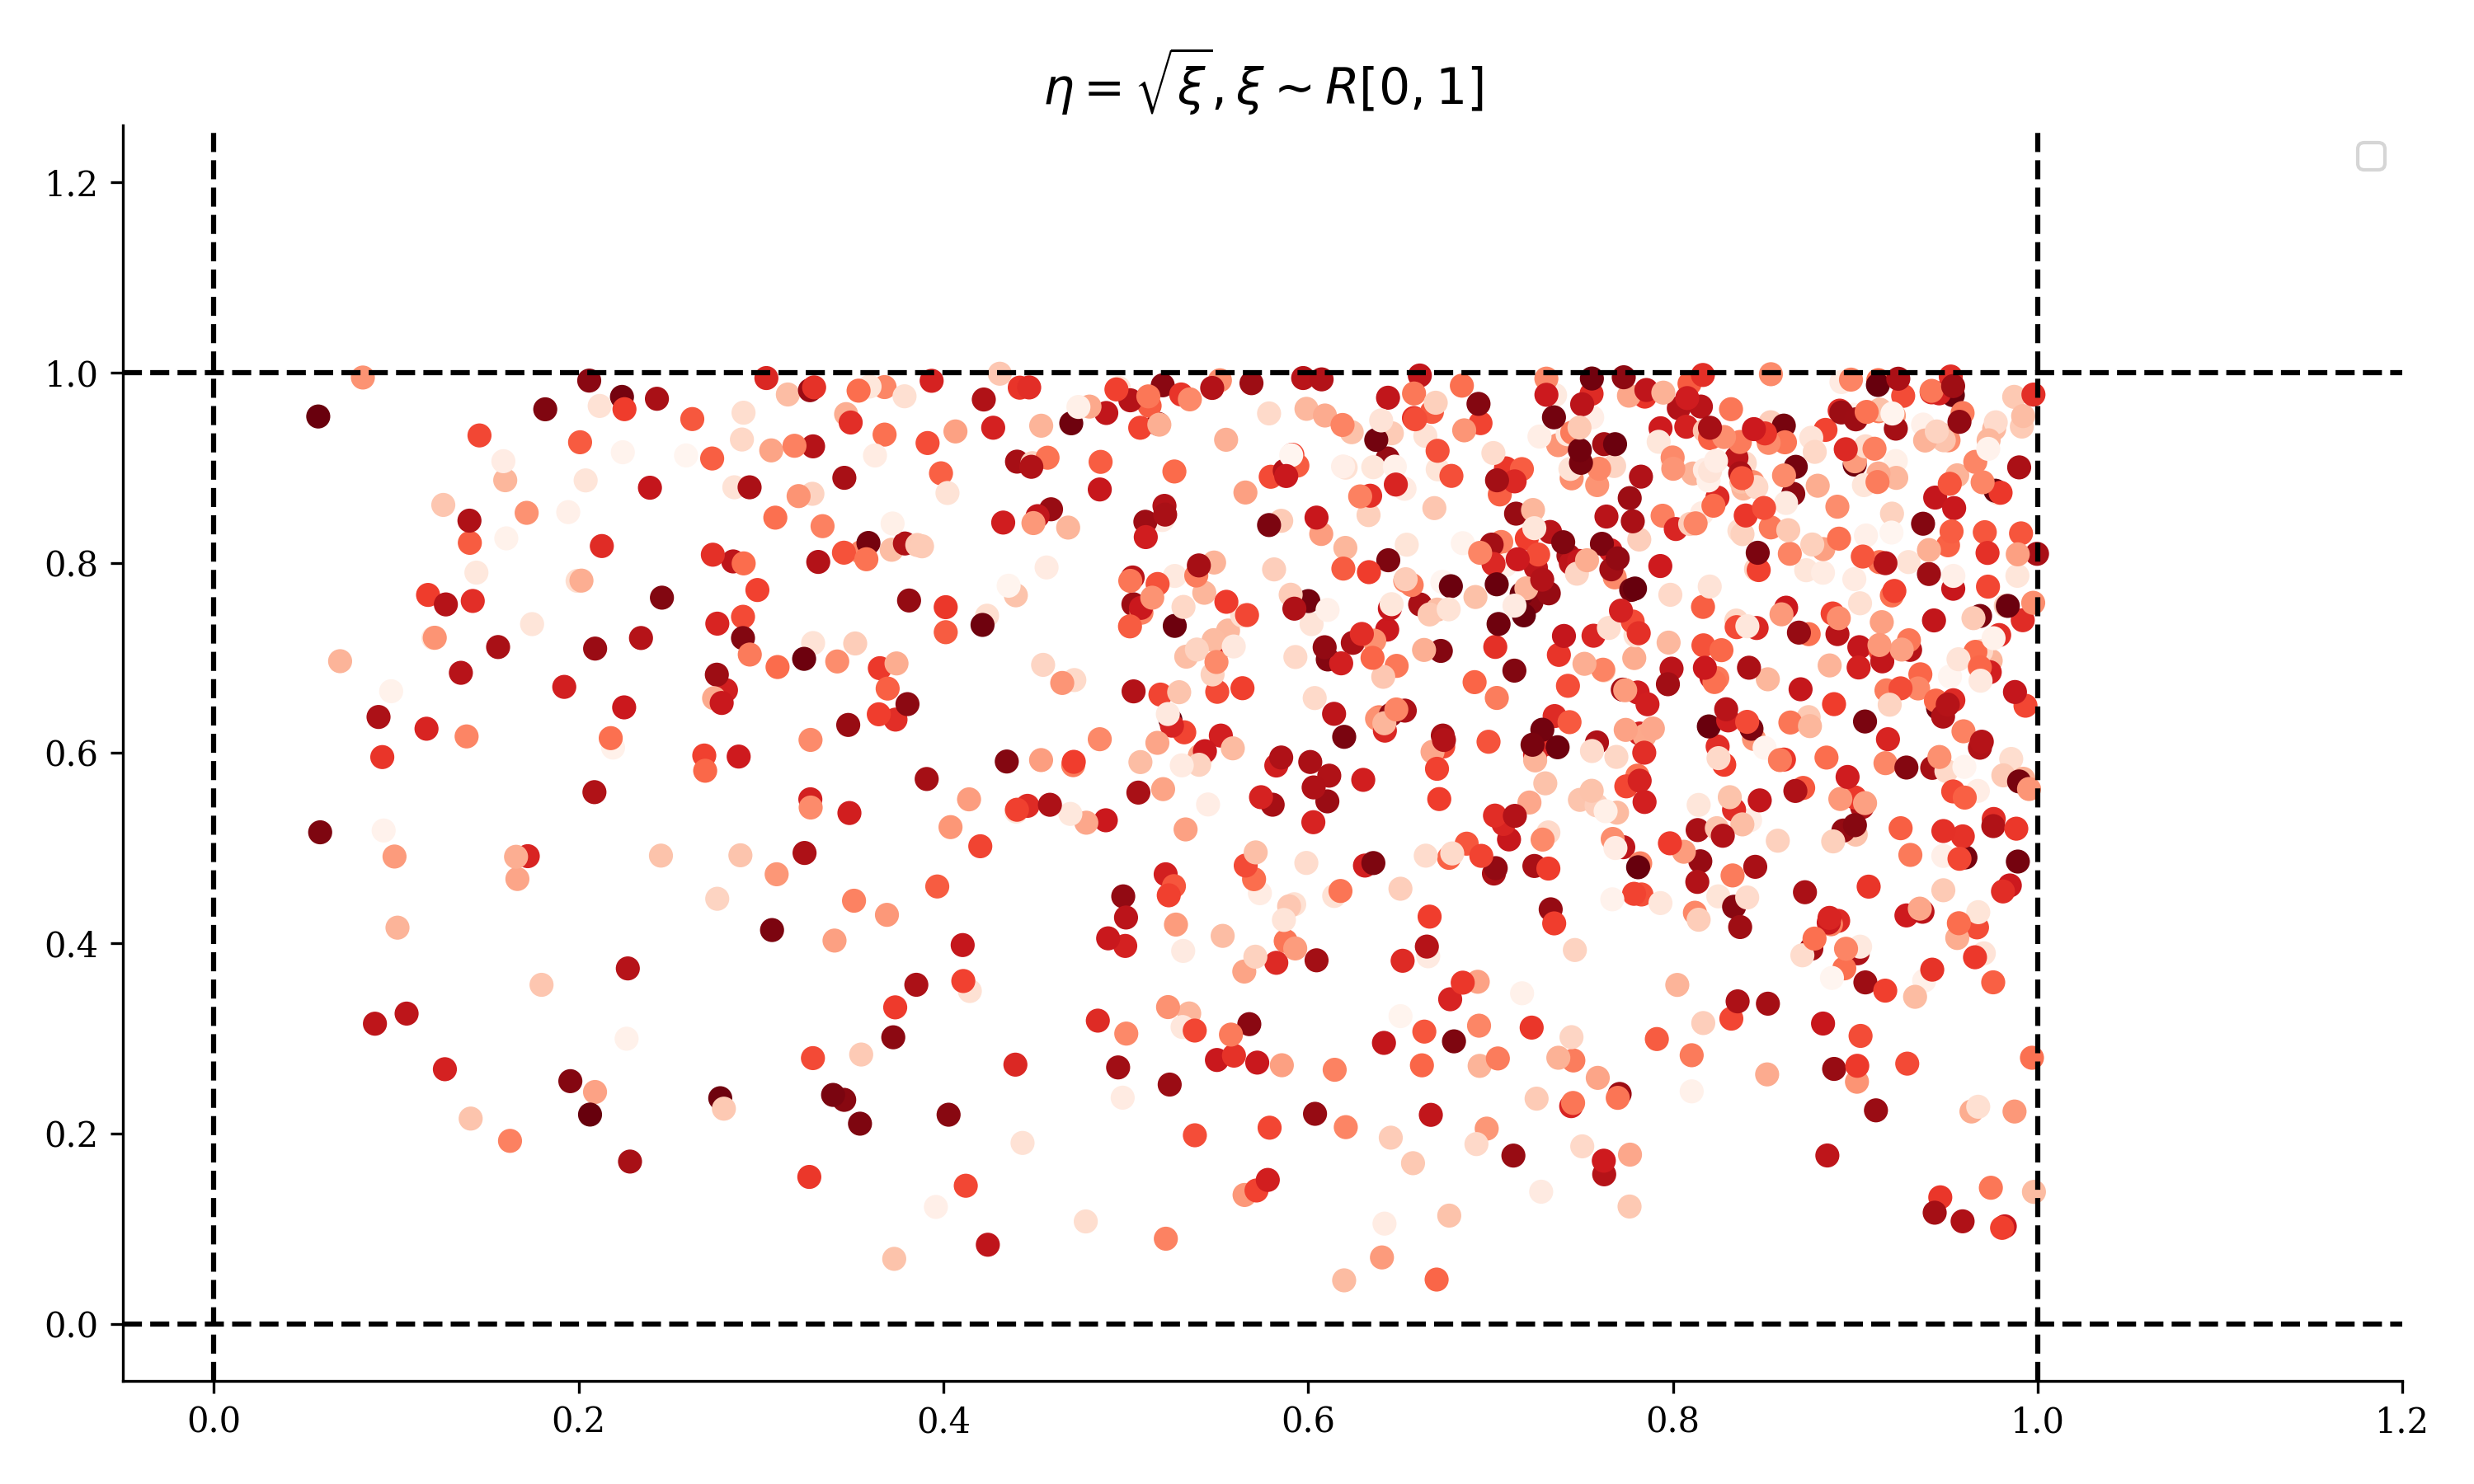
\includegraphics[width=\textwidth, height=\textheight, keepaspectratio]{modifed_uniform_EXTRA_SAMPLE_SIZE} \\
  \vspace{-10pt}
  \text{\footnotesize (Цвет не несет информации о каких-либо свойствах распределения}\\[-5pt]
  \text{\footnotesize и используется исключительно для улучшения визуального восприятия.)}
\end{center}

\begin{center}
  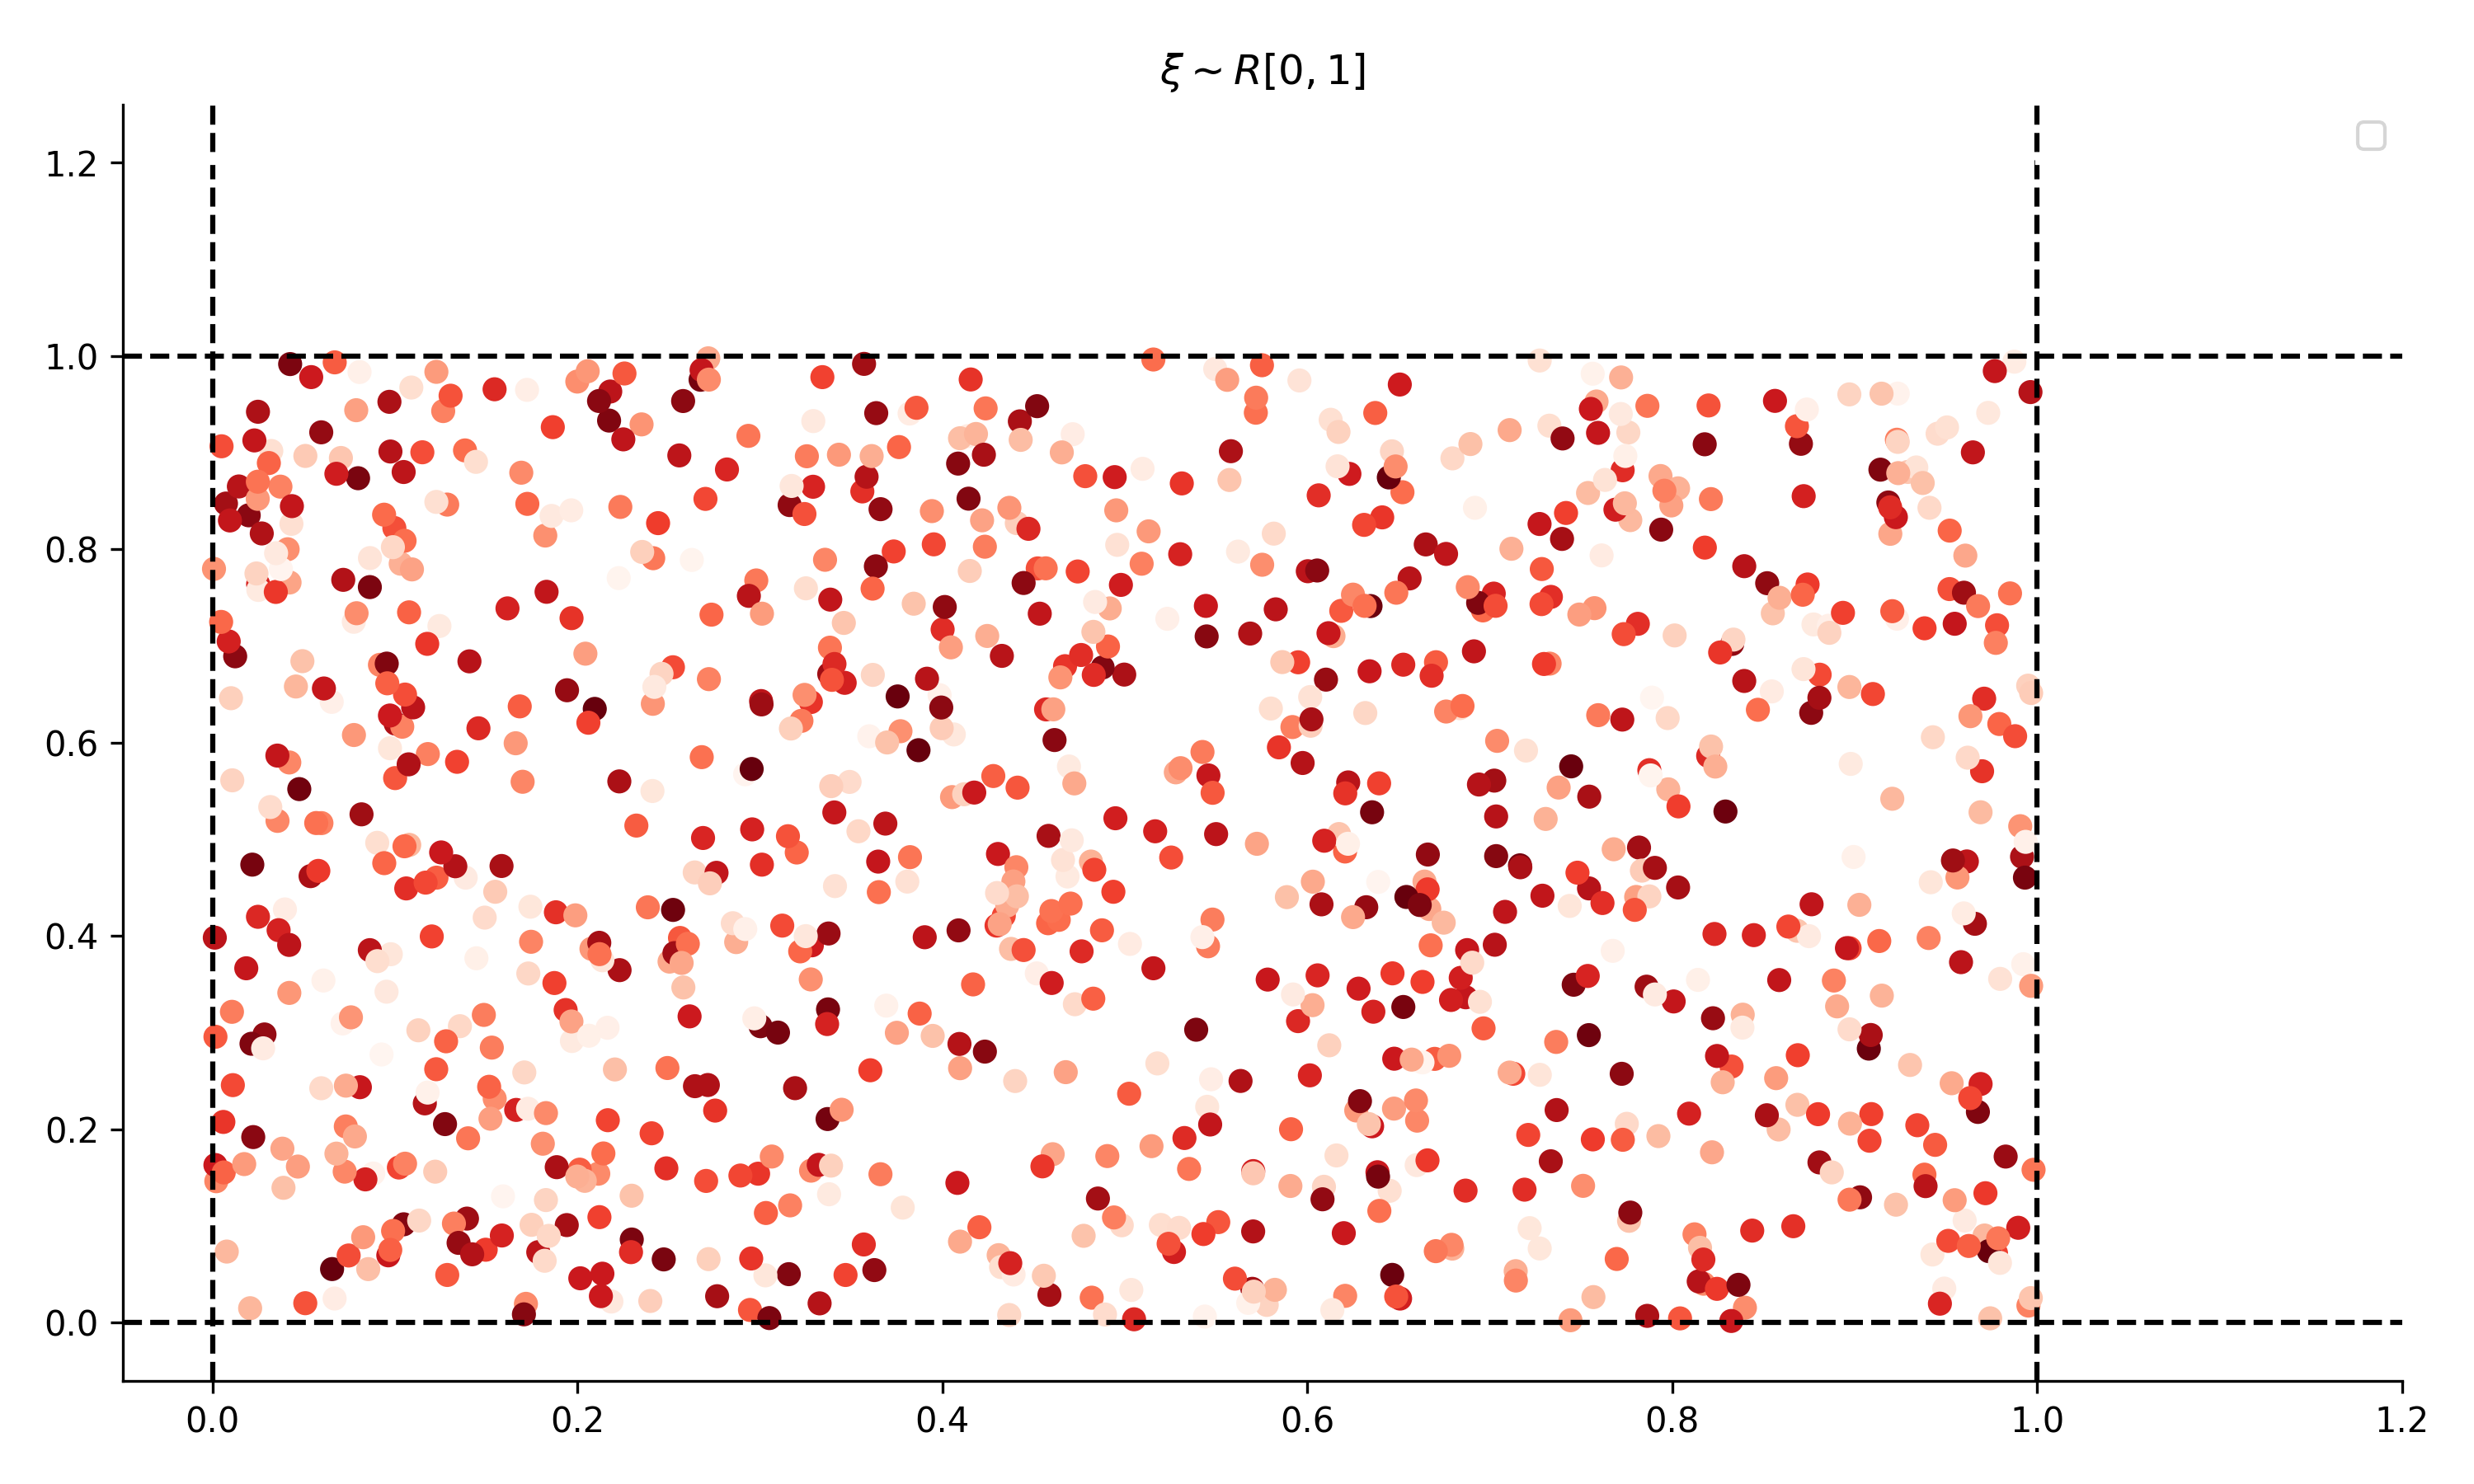
\includegraphics[width=\textwidth, height=\textheight, keepaspectratio]{uniform_EXTRA_SAMPLE_SIZE} 
  \vspace{-10pt}
  \text{\footnotesize (Цвет не несет информации о каких-либо свойствах распределения}\\[5pt]
  \text{\footnotesize и используется исключительно для улучшения визуального восприятия.)}
\end{center}

Также посмотрим на функции плотности вероятности (далее pdf) и функции распределения (далее cdf).\\

pdf и cdf для непрерывного равномерного закона на 
отрезке [0, 1] известны и равны:

\begin{gather*}
  f_X (x) = \begin{cases}
    1, \quad x \in [0, 1] \\
    0, \quad x \notin [0, 1]
  \end{cases}
  \qquad
  F_X(x) = \begin{cases}
    0, \quad x < 0 \\
    x, \quad 0 \leq x < 1 \\
    1, \quad x \geq 1
  \end{cases}
\end{gather*}

Для нахождения pdf и cdf для случайной величины 
$\eta = \sqrt{\xi}, \hspace{10pt} \xi \sim R[0, 1]$, воспользуемся формулами[1]:

\begin{equation}
  p_{\eta}(x) = \cfrac{1}{g'(g^{-1}(x))} p_{\xi}(g^{-1}(x))
\end{equation}

\begin{equation}
  F_\eta (x) = P \left\{ \eta \leq x \right\} = P \left\{ g(\xi) \leq x \right\} = 
  P \left\{ \xi \leq g^{-1}(x) \right\} = F_{\xi} (g^{-1}(x))
\end{equation}

Программно реализуем данные формулы:

\begin{center}
  \begin{lstlisting}[language=Python]
def g(x):
    match A_:
        case 1:
            return np.sqrt(x)
        case 2:
            return 1 - np.sqrt(x)
        case _:
            raise ValueError("Invalid value for A")

def inverseFunction(y):
    def equation_to_solve(x):
            return g(x) - y

    sol = None
    guesses = np.arange(a_, b_ + (b_ - a_)/10, (b_ - a_)/10)
    for guess in guesses:
        try: 
            sol, = sp.optimize.fsolve(equation_to_solve, guess)
            break
        except:
            continue
    
    if sol is not None: 
        return sol
    else: 
        raise Exception('solution was not found')
  \end{lstlisting}
\end{center}

\begin{center}
  \begin{lstlisting}[language=Python]
def pdf_(x):
    if x < a_ or x > b_:
        return 0

    def numericalDerivative(f, x):
         return cdm_.diff(f=f, x=x)
    
    inverse_x = inverseFunction(x)
    return 1 / numericalDerivative(g, inverse_x) * sp.stats.uniform.pdf(inverse_x)
  \end{lstlisting}
\end{center}

\begin{center}
  \begin{lstlisting}[language=Python]
def cdf_(x):
    return sp.stats.uniform.cdf(inverseFunction(x))
  \end{lstlisting}
\end{center}

Где для дифференцирования используется метод центральных разностей:
\begin{equation*}
  f'(x) \approx \cfrac{f(x+h) - f(x-h)}{2h}
\end{equation*}
Погрешность определяется как $O(h)$, $h$ примем равной 1e-6.\\

\begin{center}
  \begin{lstlisting}[language=Python]
class CDM:
    def __init__(self, h):
        self.h = h
    
    def diff(self, f, x):
        numerator = f(x + self.h) - f(x - self.h)
        denominator = 2 * self.h

        return numerator / denominator
  \end{lstlisting}
\end{center}

Наконец построим графики найденных pdf и cdf:

\begin{figure}[h]
  \centering
  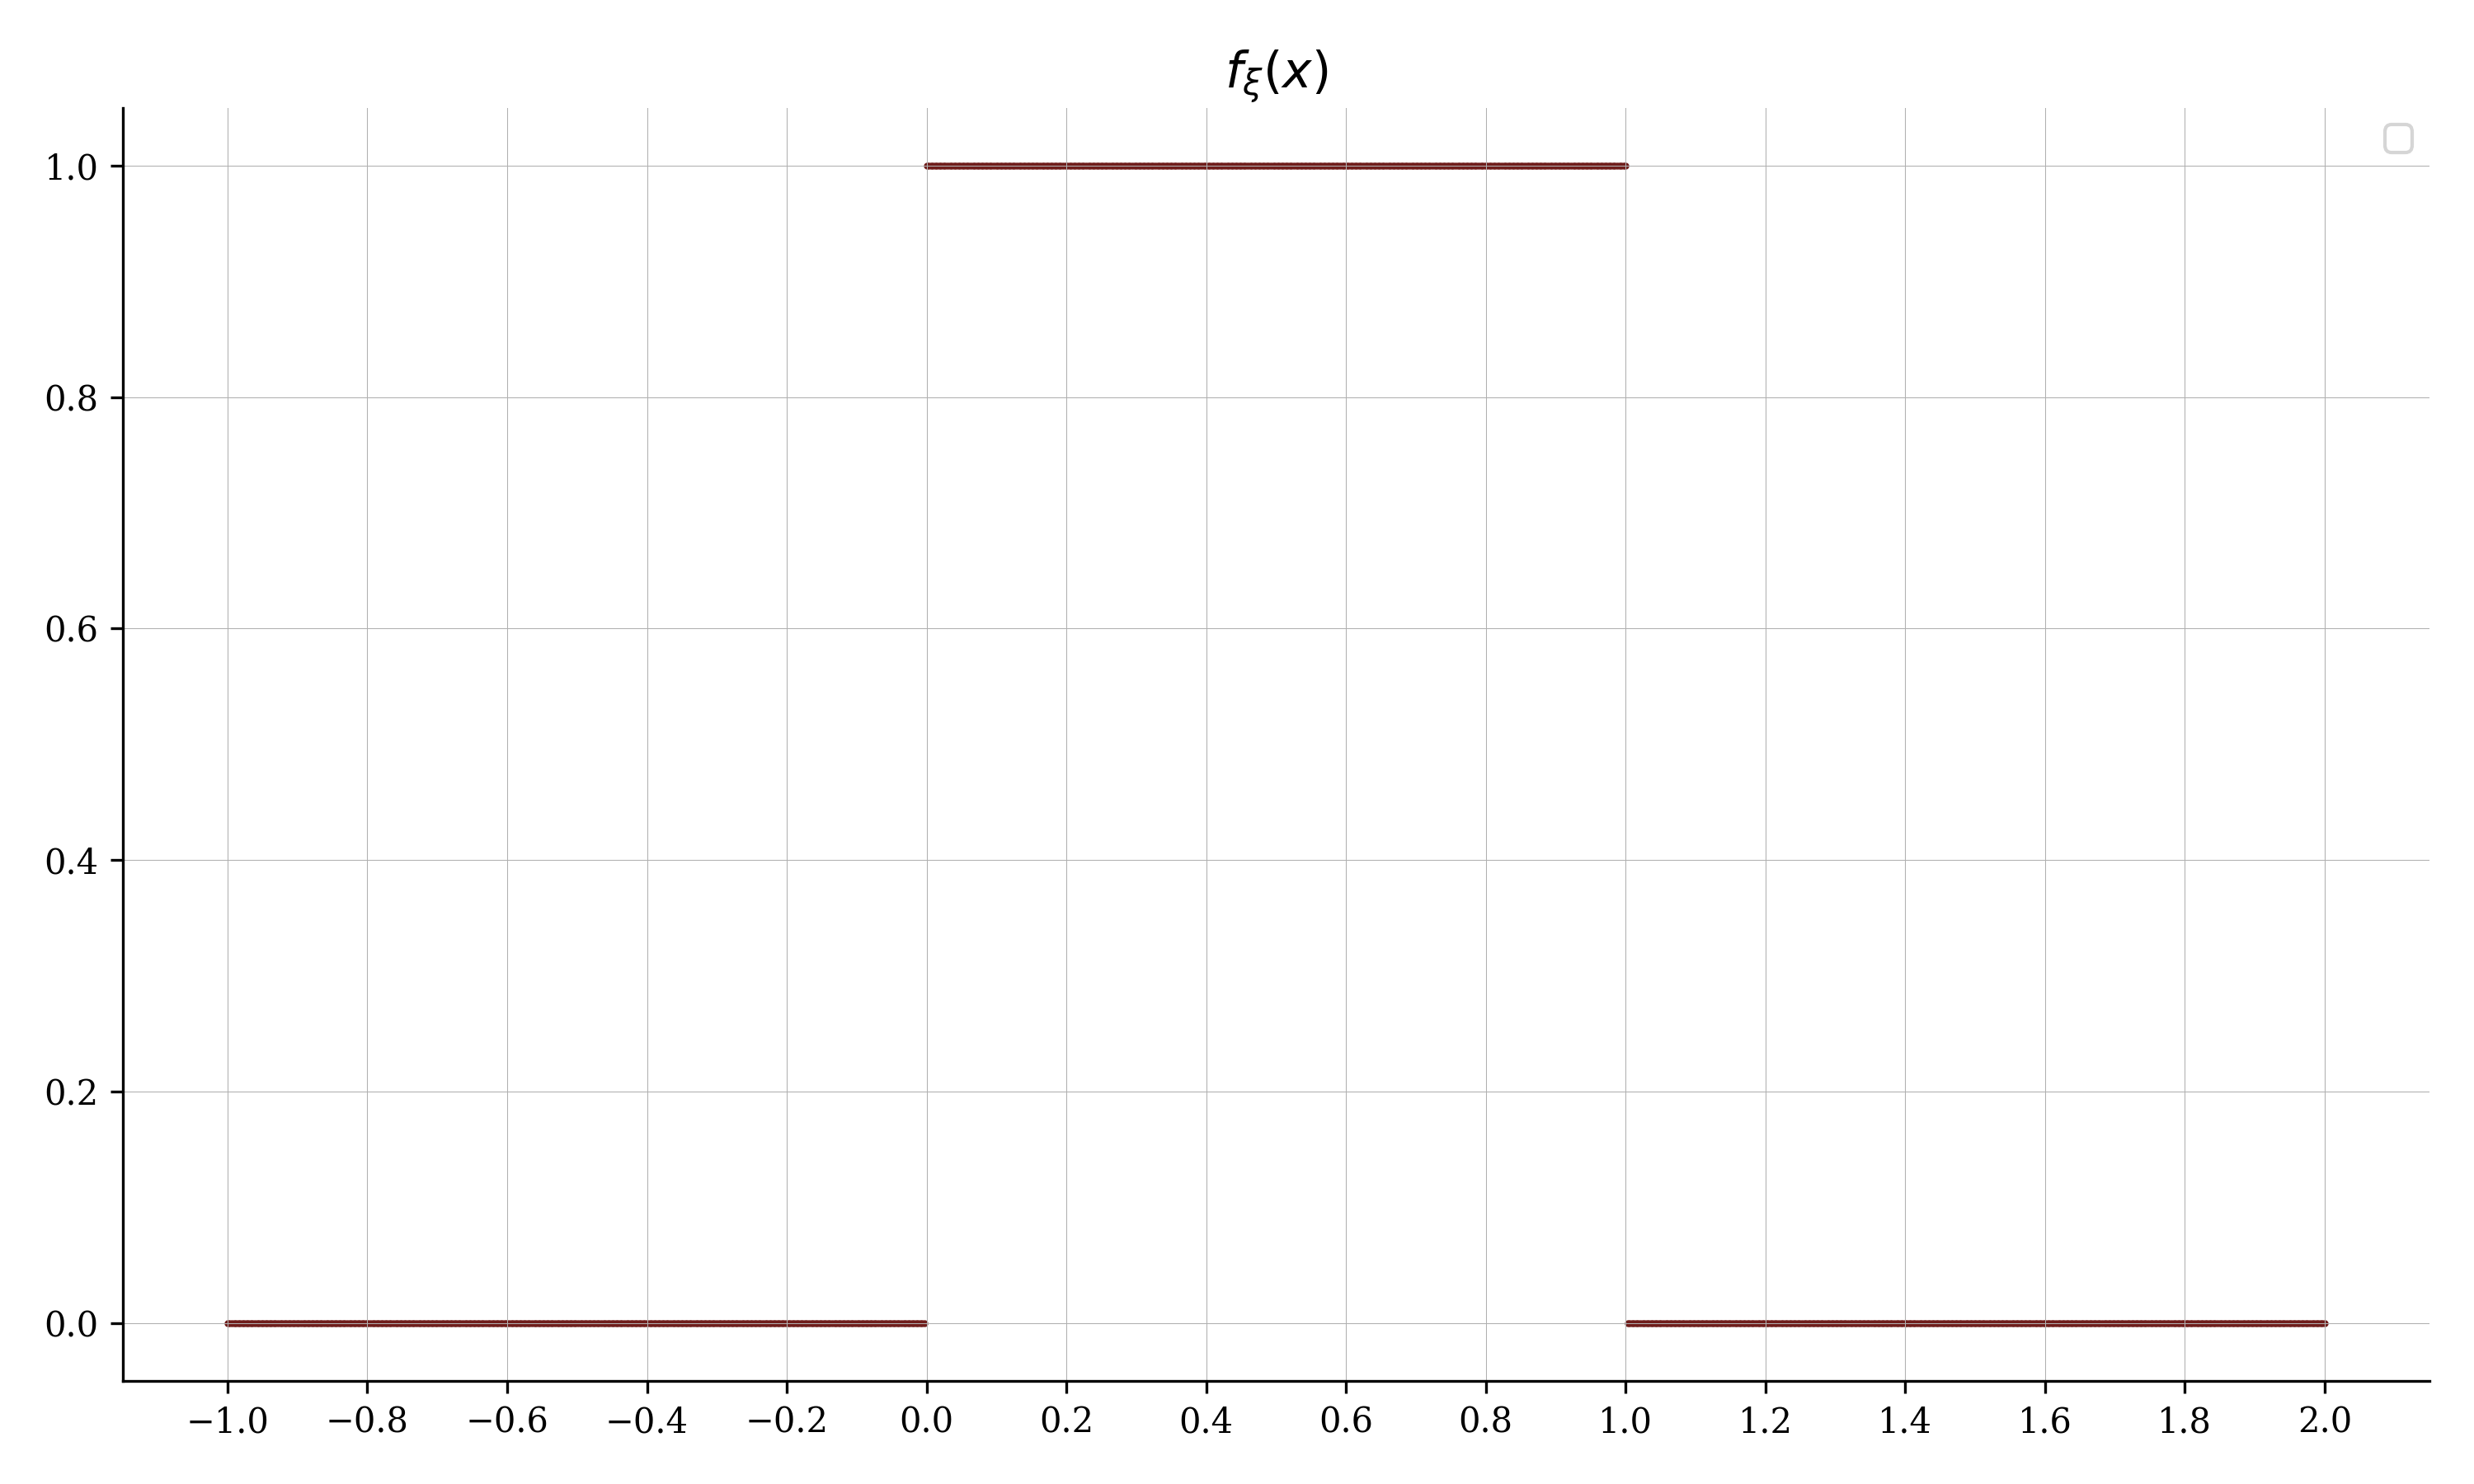
\includegraphics[width=0.45\textwidth, height=0.45\textheight, keepaspectratio]{uniform_pdf}
  \hspace{0.05\textwidth}
  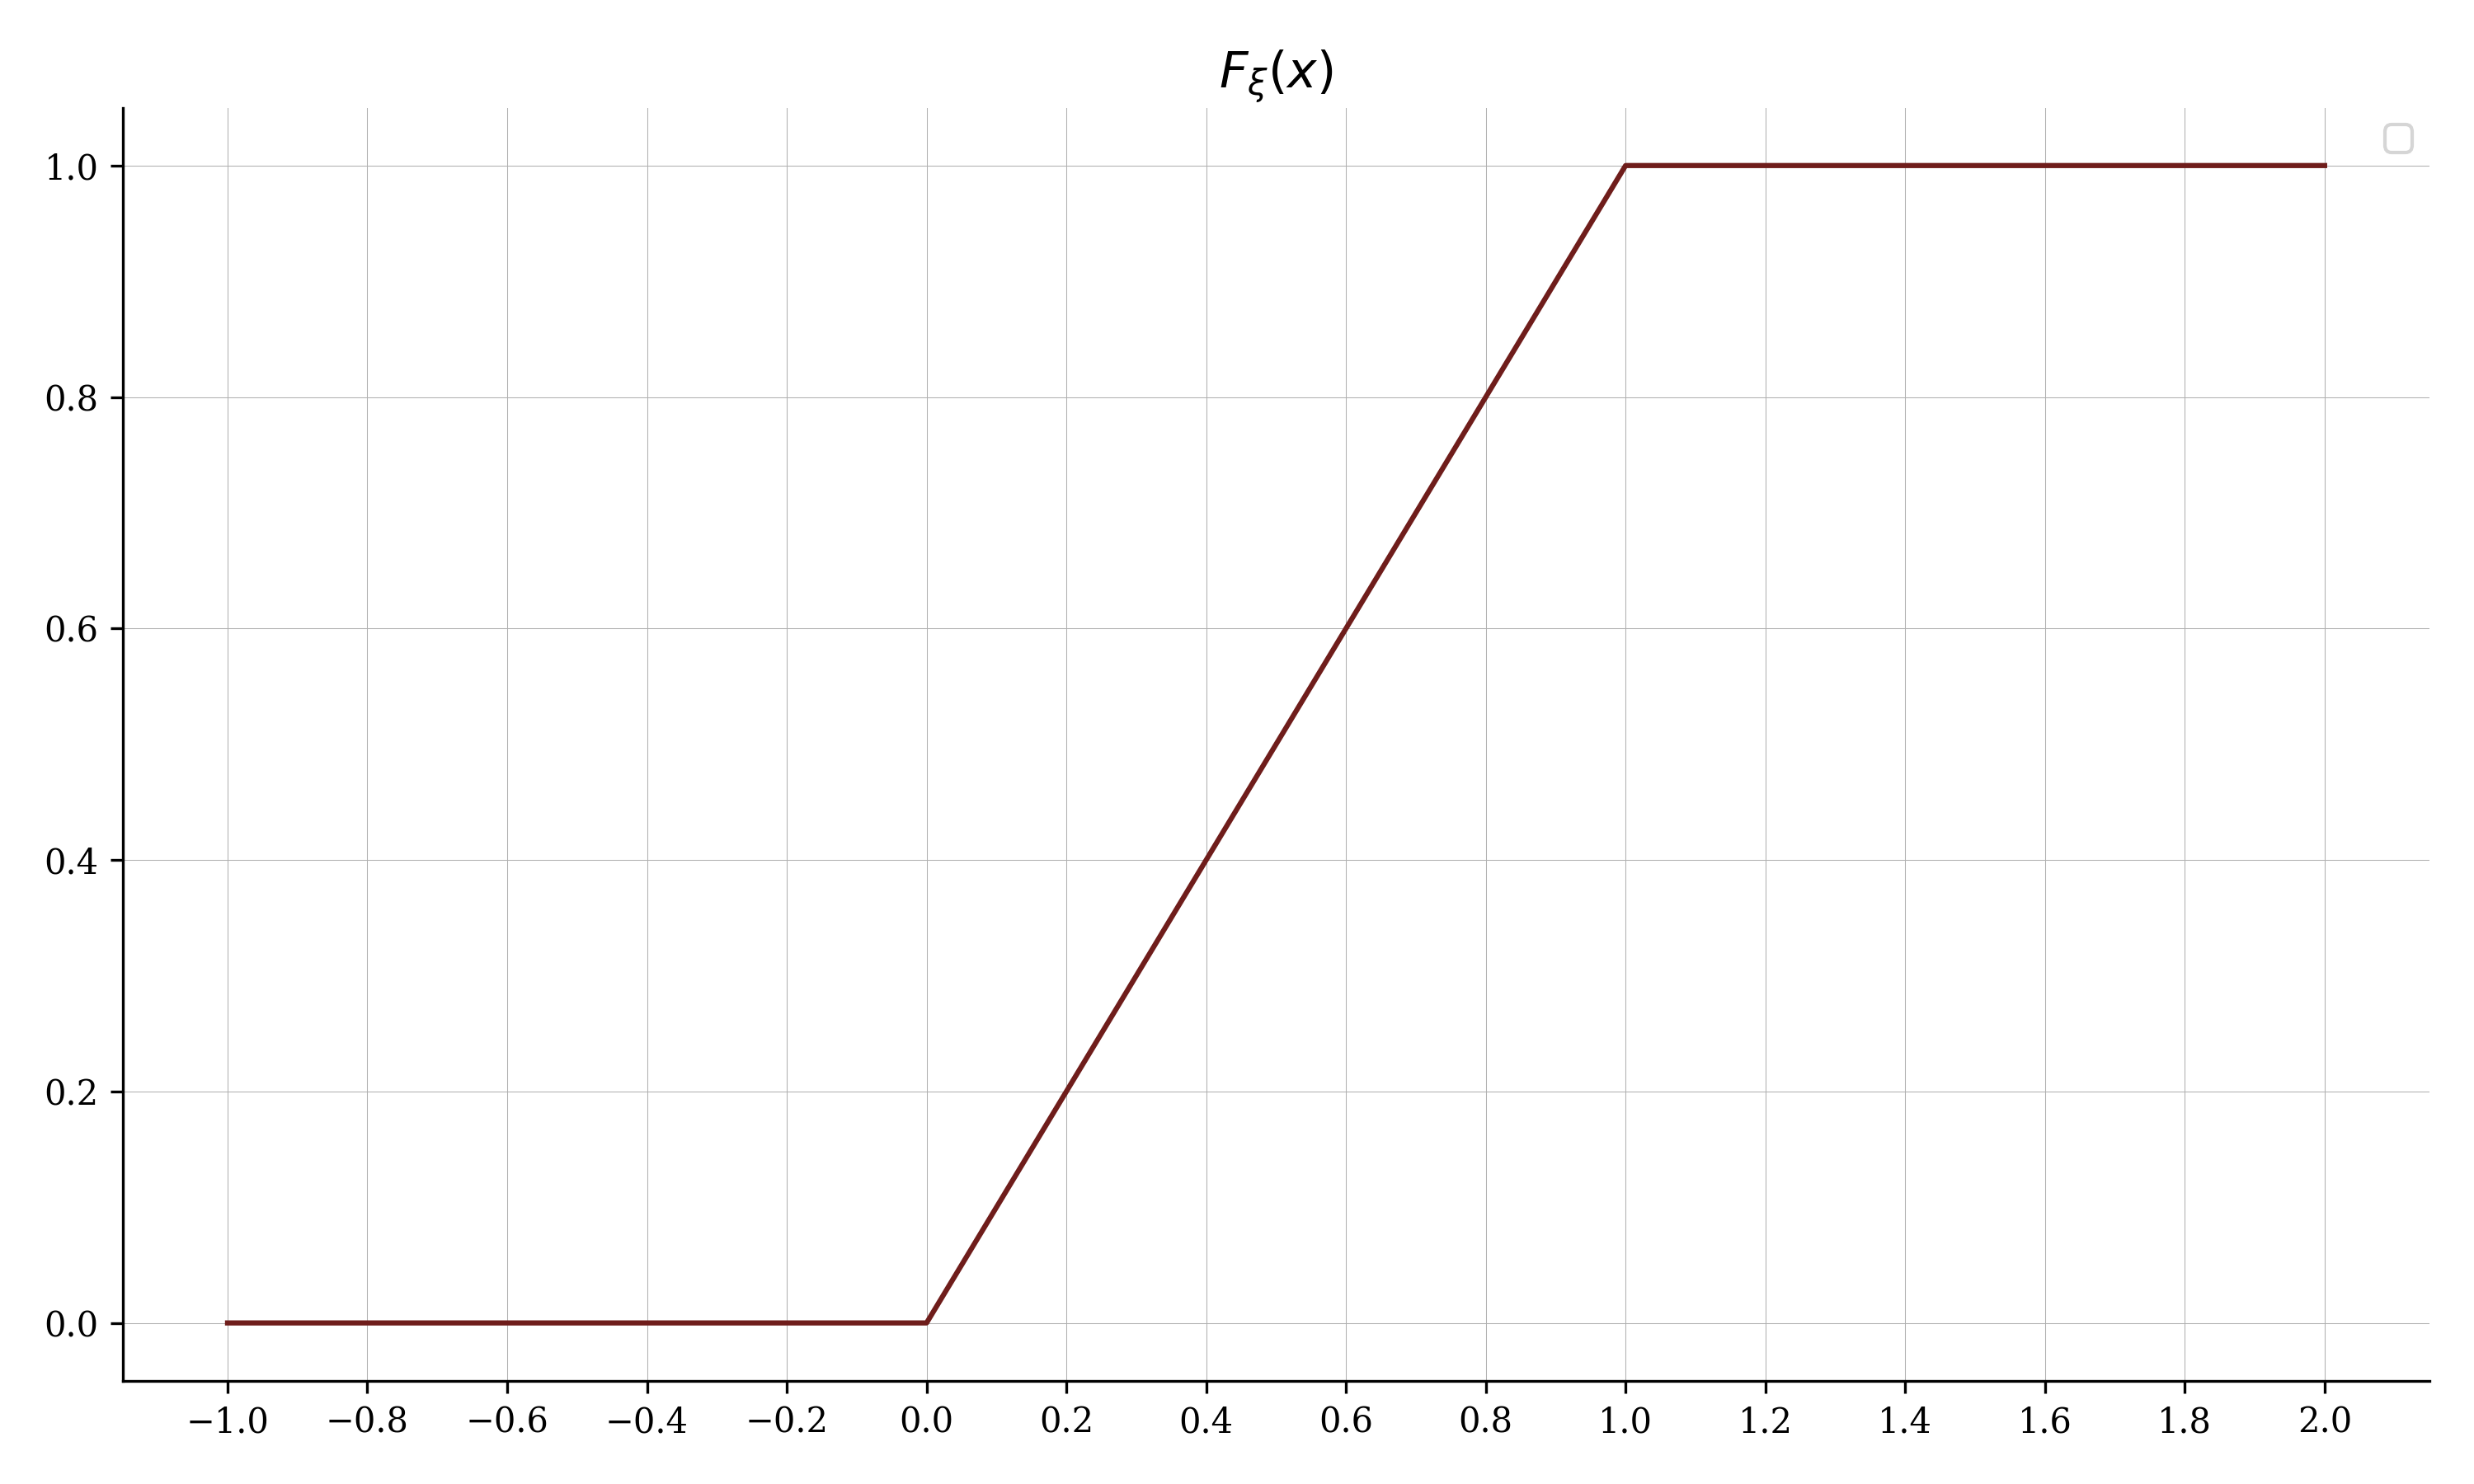
\includegraphics[width=0.45\textwidth, height=0.45\textheight, keepaspectratio]{uniform_cdf}
\end{figure}

\begin{figure}[h]
  \centering
  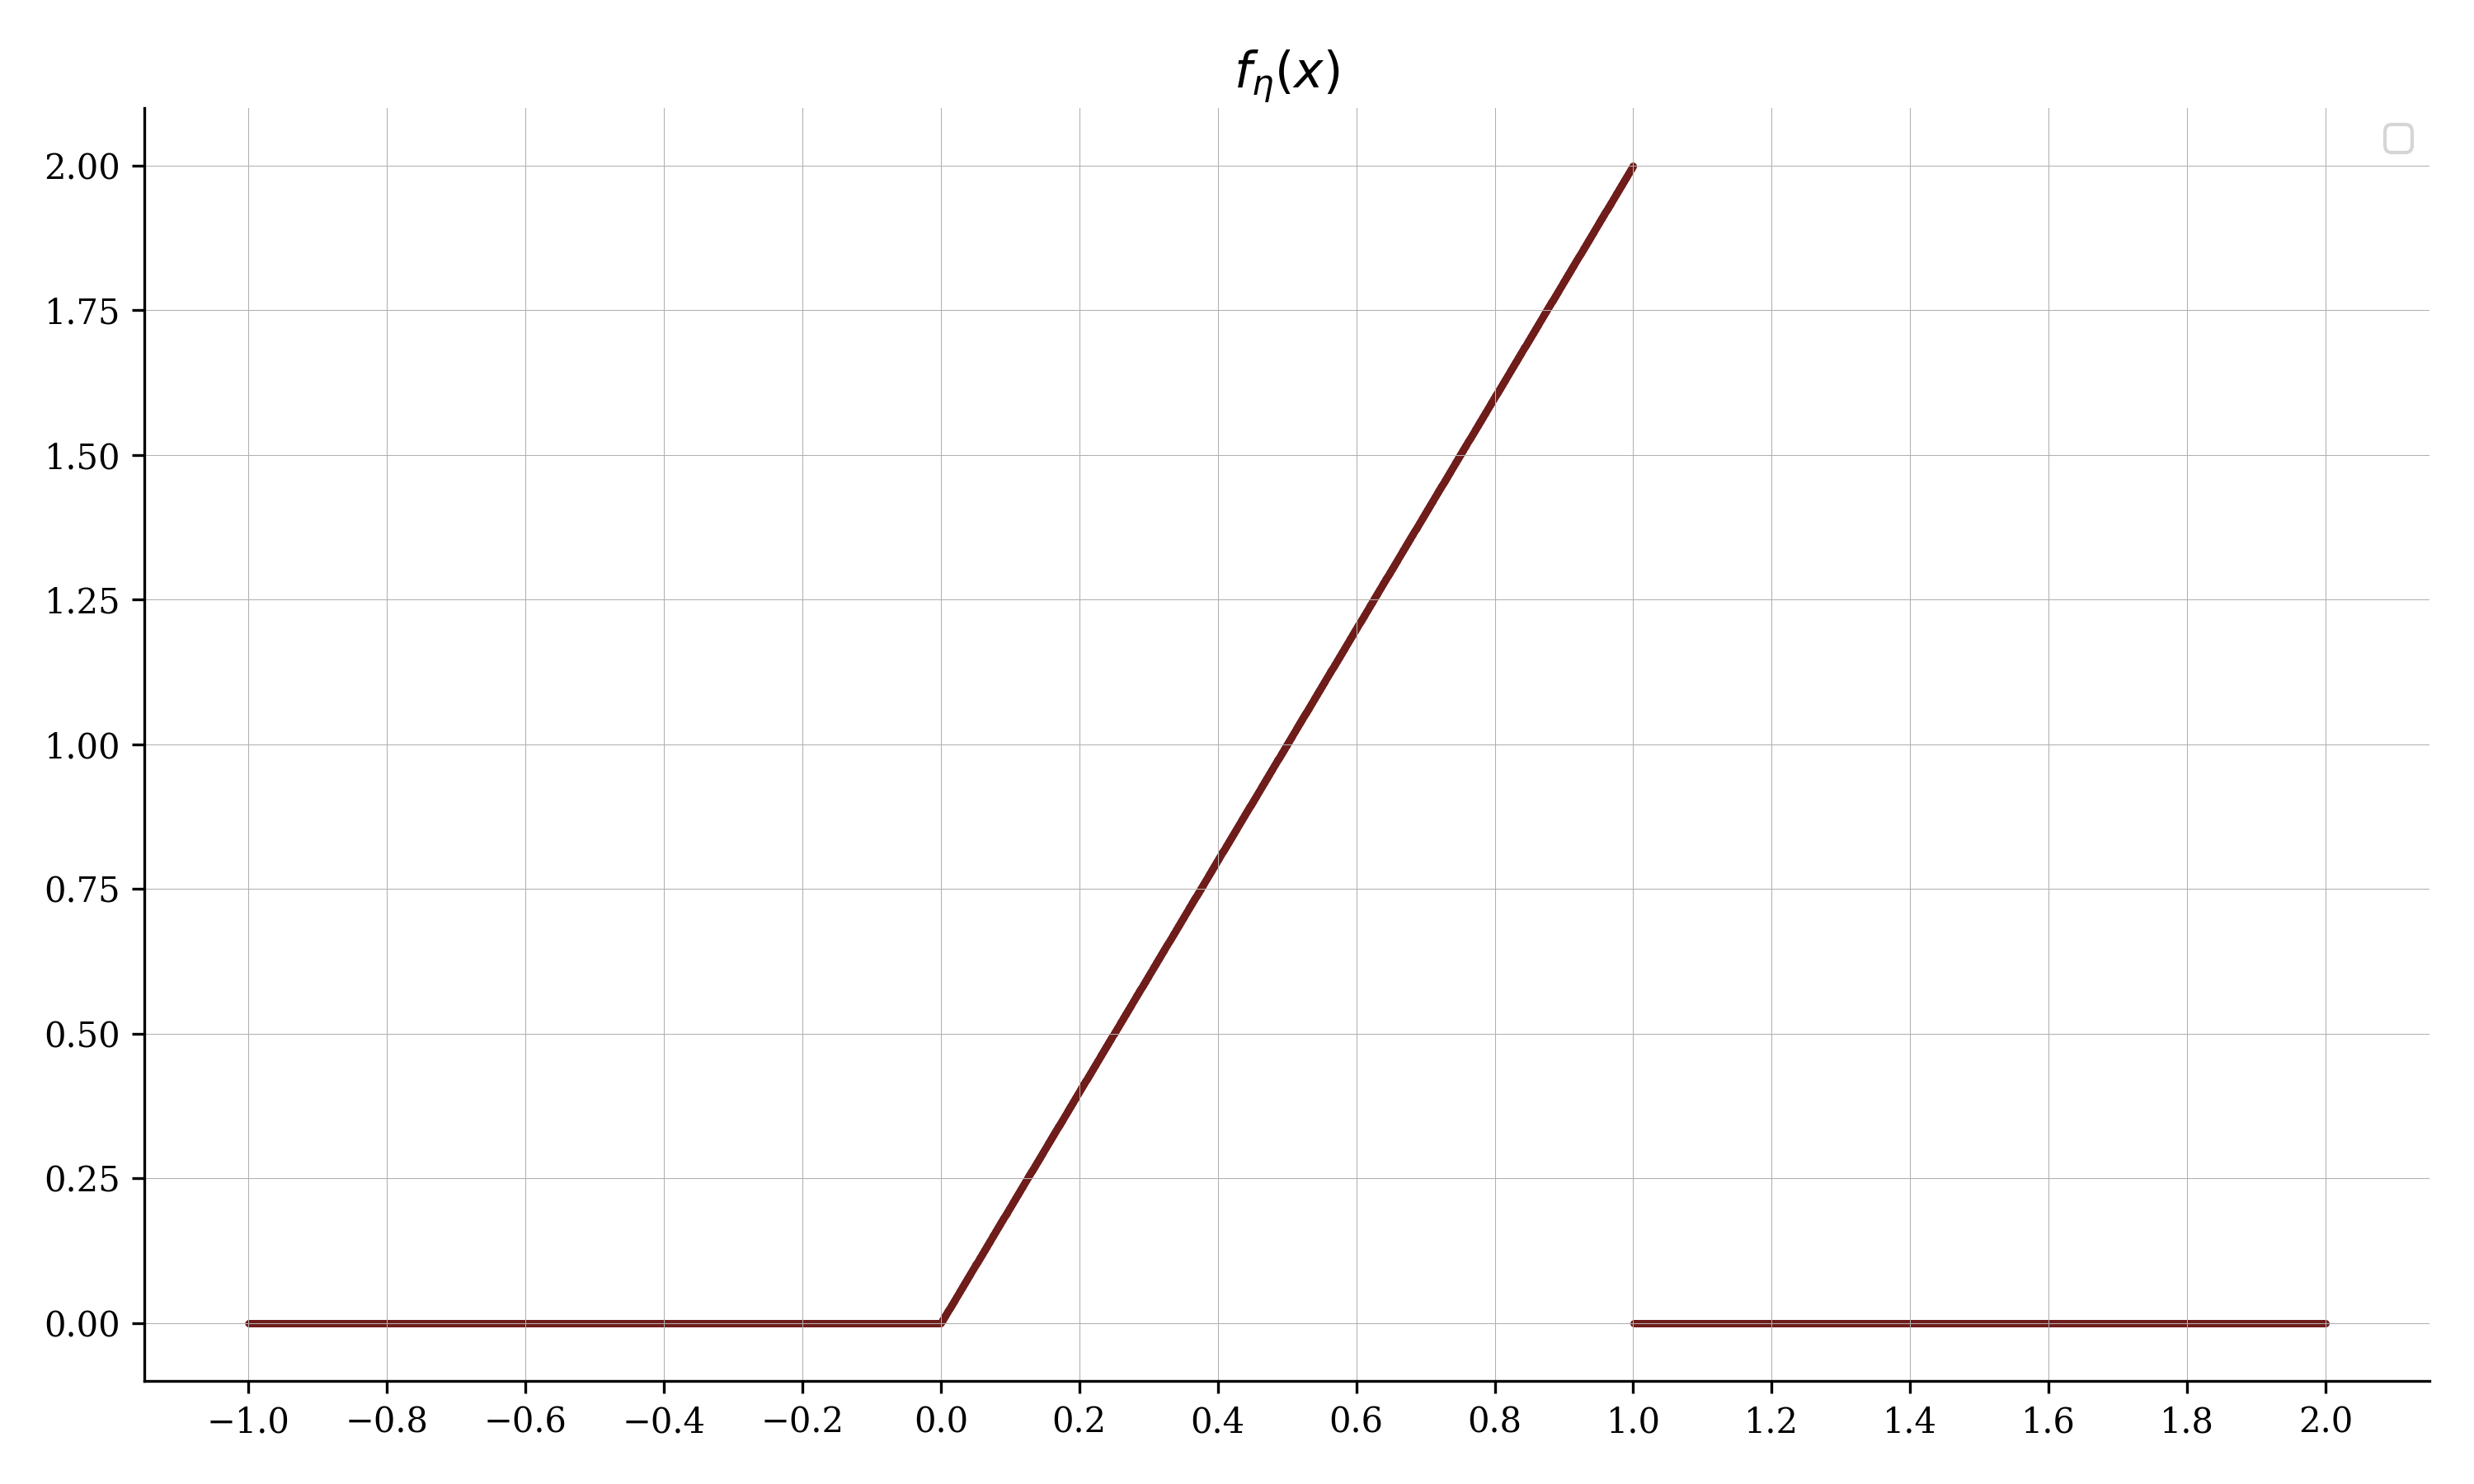
\includegraphics[width=0.45\textwidth, height=0.45\textheight, keepaspectratio]{modified_uniform_pdf}
  \hspace{0.05\textwidth}
  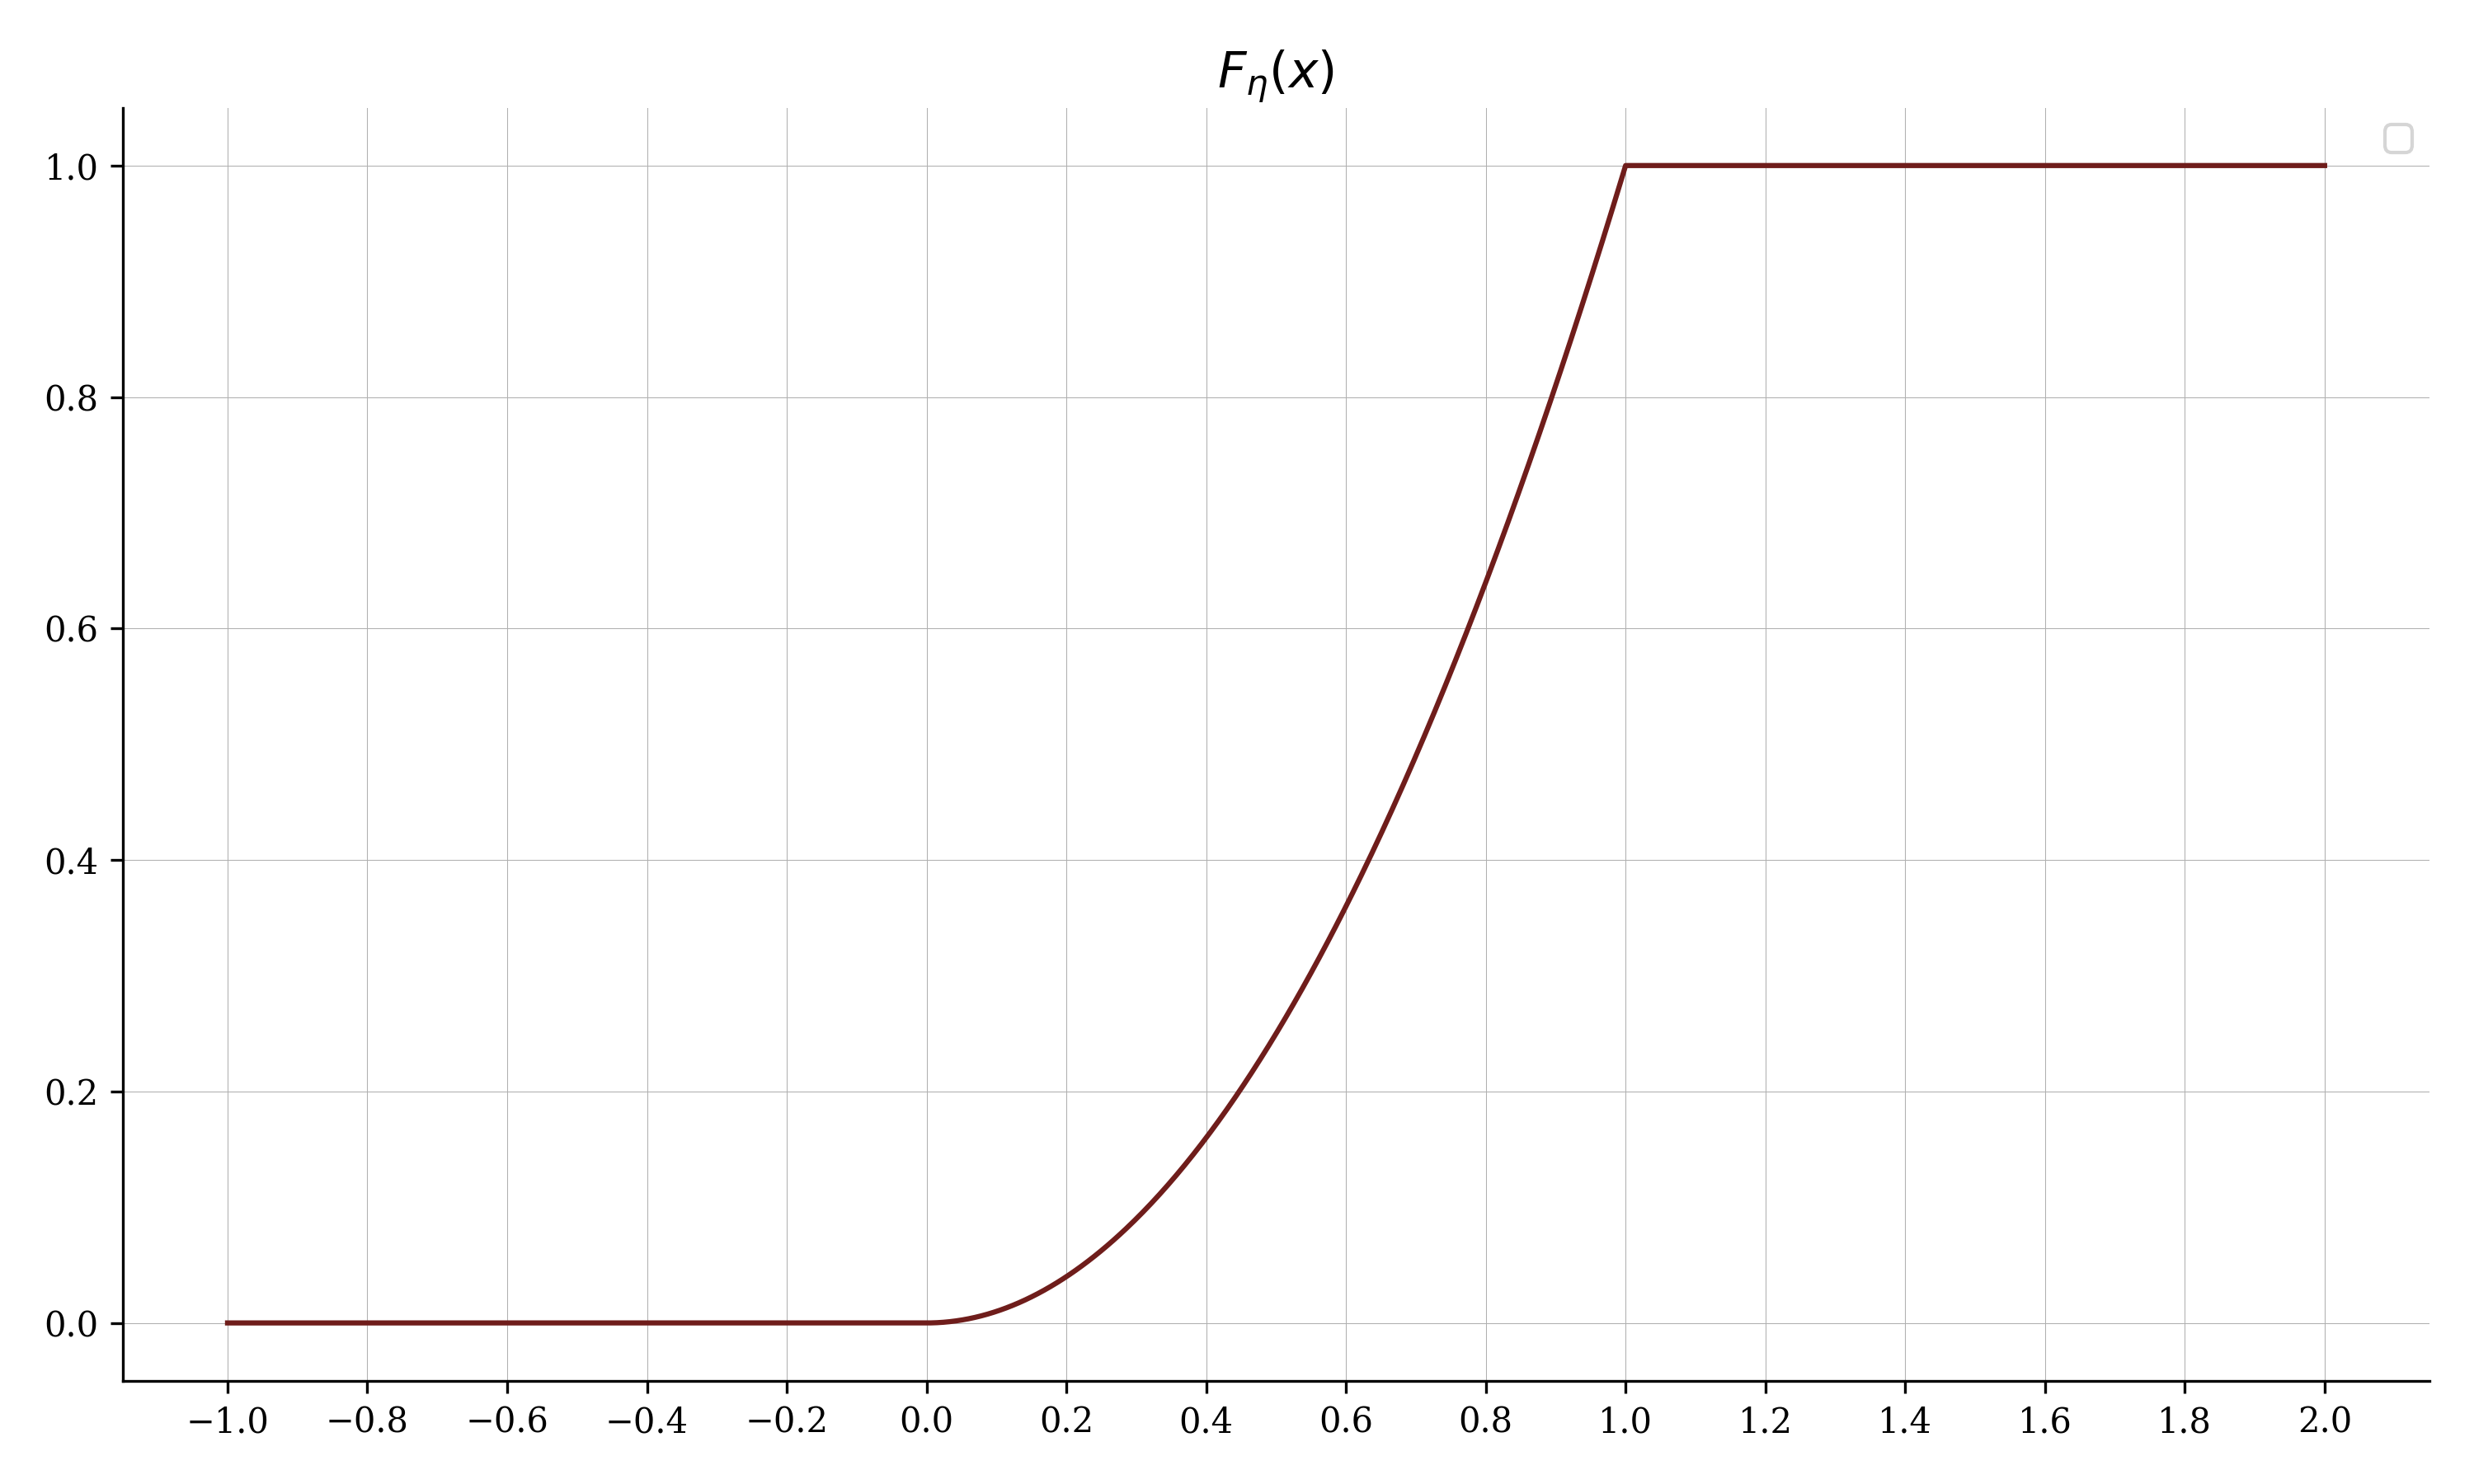
\includegraphics[width=0.45\textwidth, height=0.45\textheight, keepaspectratio]{modifed_uniform_cdf}
\end{figure}

Перейдем к стохастическому эксперименту.\\
Напишем вспомогательную функцию для генерации выборки, в соответствии с вариантом:

\begin{center}
  \begin{lstlisting}[language=Python]
def generateValue(n=1):
    match A_:
        case 0:
            return sp.stats.uniform.rvs(size=n)
        case 1:
            return np.sqrt(sp.stats.uniform.rvs(size=n))
        case 2:
            return 1 - np.sqrt(sp.stats.uniform.rvs(size=n))
  \end{lstlisting}
\end{center}

Теперь смоделируем выборку, подчиняющуюся основной гипотезе m = 1e4 раз:

\begin{center}
  \begin{lstlisting}[language=Python]
data_ = [generateValue(n_) for _ in range(m_)]
  \end{lstlisting}
\end{center}

Сгруппируем каждую из полученных выборок. 

Для этого создадим вспомогательный класс \high{Sample}, который будет хранить 
следующие параметры как поля класса:

размер выборки ($\_n$), крайние члены ($\_min$ и $\_max$), размах выборки ($\_range$),
количество интервалов ($\_l$), шаг интервала ($\_h$), границы интервалов ($\_int\_boundaries$),
интервалы ($\_intervals$), середины интервалов ($\_mid\_ranges$), частоты ($\_freqs$),
относительные частоты ($\_rel\_freqs$) и плотность относительных частот ($\_rel\_freqs\_density$).\\

Следующие поля сделаем статическими, тк они остаются постоянными вне зависимости от выборки:\\
$\_n$, $\_min$, $\_max$, $\_range$, $\_l$, $\_h$, $\_int\_boundaries$, $\_intervals$, $\_mid\_ranges$.\\

Которые инициализируем в отдельном методе:
\begin{center}
  \begin{lstlisting}[language=Python]
@classmethod
def _initializeStaticFields(cls):
    cls._n     = n_
    cls._min   = a_
    cls._max   = b_
    cls._range = cls._max - cls._min
    cls._l     = 1 + int(np.log2(cls._n))
    cls._h     = cls._range / cls._l
    
    cls._int_boundaries = np.array(
        [cls._min + i * cls._h for i in range(0, cls._l + 1, 1)]
    )
    cls._intervals = np.array(
        [(cls._int_boundaries[i], 
          cls._int_boundaries[i+1]) for i in range(0, cls._l, 1)]
    )
    cls._mid_ranges = np.array(
        [sum(interval)/2 for interval in cls._intervals]
    )
  \end{lstlisting}
\end{center}

Также отдельно напишем обработку частот, так как они уже будут разниться у каждой выборки:
\begin{center}
  \begin{lstlisting}[language=Python]
def _countFrequencies(self, data):
    present = lambda el, int_ : int_[0] <= el < int_[1]
    freqs_ = np.zeros(Sample._l)
    for el in data:
        for j in range(0, Sample._l, 1):
            if present(el, Sample._intervals[j]):
                freqs_[j] += 1 
    freqs_[-1] += np.count_nonzero(data == Sample._max)

    self._freqs = freqs_
    self._postCountFrequencies()

def _postCountFrequencies(self):
    if self._freqs is not None:
        rel_freqs_ = self._freqs / Sample._n

        self._rel_freqs = rel_freqs_

        rel_freqs_density_ = self._rel_freqs / Sample._h
        self._rel_freqs_density = rel_freqs_density_
  \end{lstlisting}
\end{center}

\newpage

Наконец сгруппируем каждую из m сгенерированных выборок:
\begin{center}
  \begin{lstlisting}[language=Python]
groupedSamples = [Sample(sample) for sample in data_]
  \end{lstlisting}
\end{center}

Выведем информацию о полученной группировке для одной из выборок.

Данная информация присуща всем выборкам:
\begin{gather*}
  \text{n}: 1000 \qquad \text{min}: 0 \qquad \text{max}: 1 \qquad \text{range}: 1 \qquad \text{l}: 10 \qquad \text{h}: 0.1 \\
\end{gather*}
\vspace{-60pt}
\begin{flalign*}
  & \text{границы интервалов}: [0 \hspace{10pt} 0.1 \hspace{10pt} 0.2 \hspace{10pt} 0.3 \hspace{10pt} 0.4 \hspace{10pt} 0.5 \hspace{10pt} 0.6 \hspace{10pt} 0.7 \hspace{10pt} 0.8 \hspace{10pt} 0.9 \hspace{10pt} 1] \\
  & \text{интервалы}: [0 \hspace{10pt} 0.1), \hspace{10pt} [0.1 \hspace{10pt} 0.2), \hspace{10pt} [0.2 \hspace{10pt} 0.3), \hspace{10pt} [0.3 \hspace{10pt} 0.4), \hspace{10pt} [0.4 \hspace{10pt} 0.5), \\ 
  & [0.5 \hspace{10pt} 0.6), \hspace{10pt} [0.6 \hspace{10pt} 0.7), \hspace{10pt} [0.7 \hspace{10pt} 0.8), \hspace{10pt} [0.8 \hspace{10pt} 0.9), \hspace{10pt} [0.9 \hspace{10pt} 0.1] \\
  & \text{середины интервалов}: [0.05 \hspace{10pt} 0.15 \hspace{10pt} 0.25 \hspace{10pt} 0.35 \hspace{10pt} 0.45 \hspace{10pt} 0.55 \hspace{10pt} 0.65 \hspace{10pt} 0.75 \hspace{10pt} 0.85 \hspace{10pt} 0.95] \\
\end{flalign*}

Данная информация присуща только конкретной (выбранной для демонстрации) выборке:
\begin{flalign*}
  & \text{частоты}: [11 \hspace{10pt} 36 \hspace{10pt} 49 \hspace{10pt} 73 \hspace{10pt} 92 \hspace{10pt} 116 \hspace{10pt} 117 \hspace{10pt} 146 \hspace{10pt} 161 \hspace{10pt} 199] \\
  & \text{относительные частоты}: [0.011 \hspace{10pt} 0.036 \hspace{10pt} 0.049 \hspace{10pt} 0.073 \hspace{10pt} 0.092 \hspace{10pt} 0.116 \hspace{10pt} 0.117 \hspace{10pt} 0.146 \hspace{10pt} 0.161 \hspace{10pt} 0.199] \\
  & \text{плотность относительных частот}: [0.11 \hspace{10pt} 0.36 \hspace{10pt} 0.49 \hspace{10pt} 0.73 \hspace{10pt} 0.92 \hspace{10pt} 1.16 \hspace{10pt} 1.17 \hspace{10pt} 1.46 \hspace{10pt} 1.61 \hspace{10pt} 1.99] \\
\end{flalign*}

Добавим еще один метод в класс \high{Sample} для отрисовки гистограммы относительных частот:
\begin{center}
  \begin{lstlisting}[language=Python]
def _hist(self, filename):
    RED = '#6F1D1B'

    _, ax = plt.subplots(figsize=(10, 6))

    x_values = Sample._mid_ranges
    y_values = self._rel_freqs_density

    ax.bar(x_values, 
            y_values, 
            width=Sample._h, 
            color='white',
            edgecolor=RED, 
            linestyle='-', 
            linewidth=1.5, 
            align='center')

    decorate_plot(ax, Sample._int_boundaries, 'int', '$p^r$', loc=(0, 0))

    if SAVE_PLOTS:
        plt.savefig(f'{filename}.png', dpi=300, transparent=True)

    plt.show()
  \end{lstlisting}
\end{center}

Гистограмма, выбранной для демонстрации выборки:
\begin{center}
  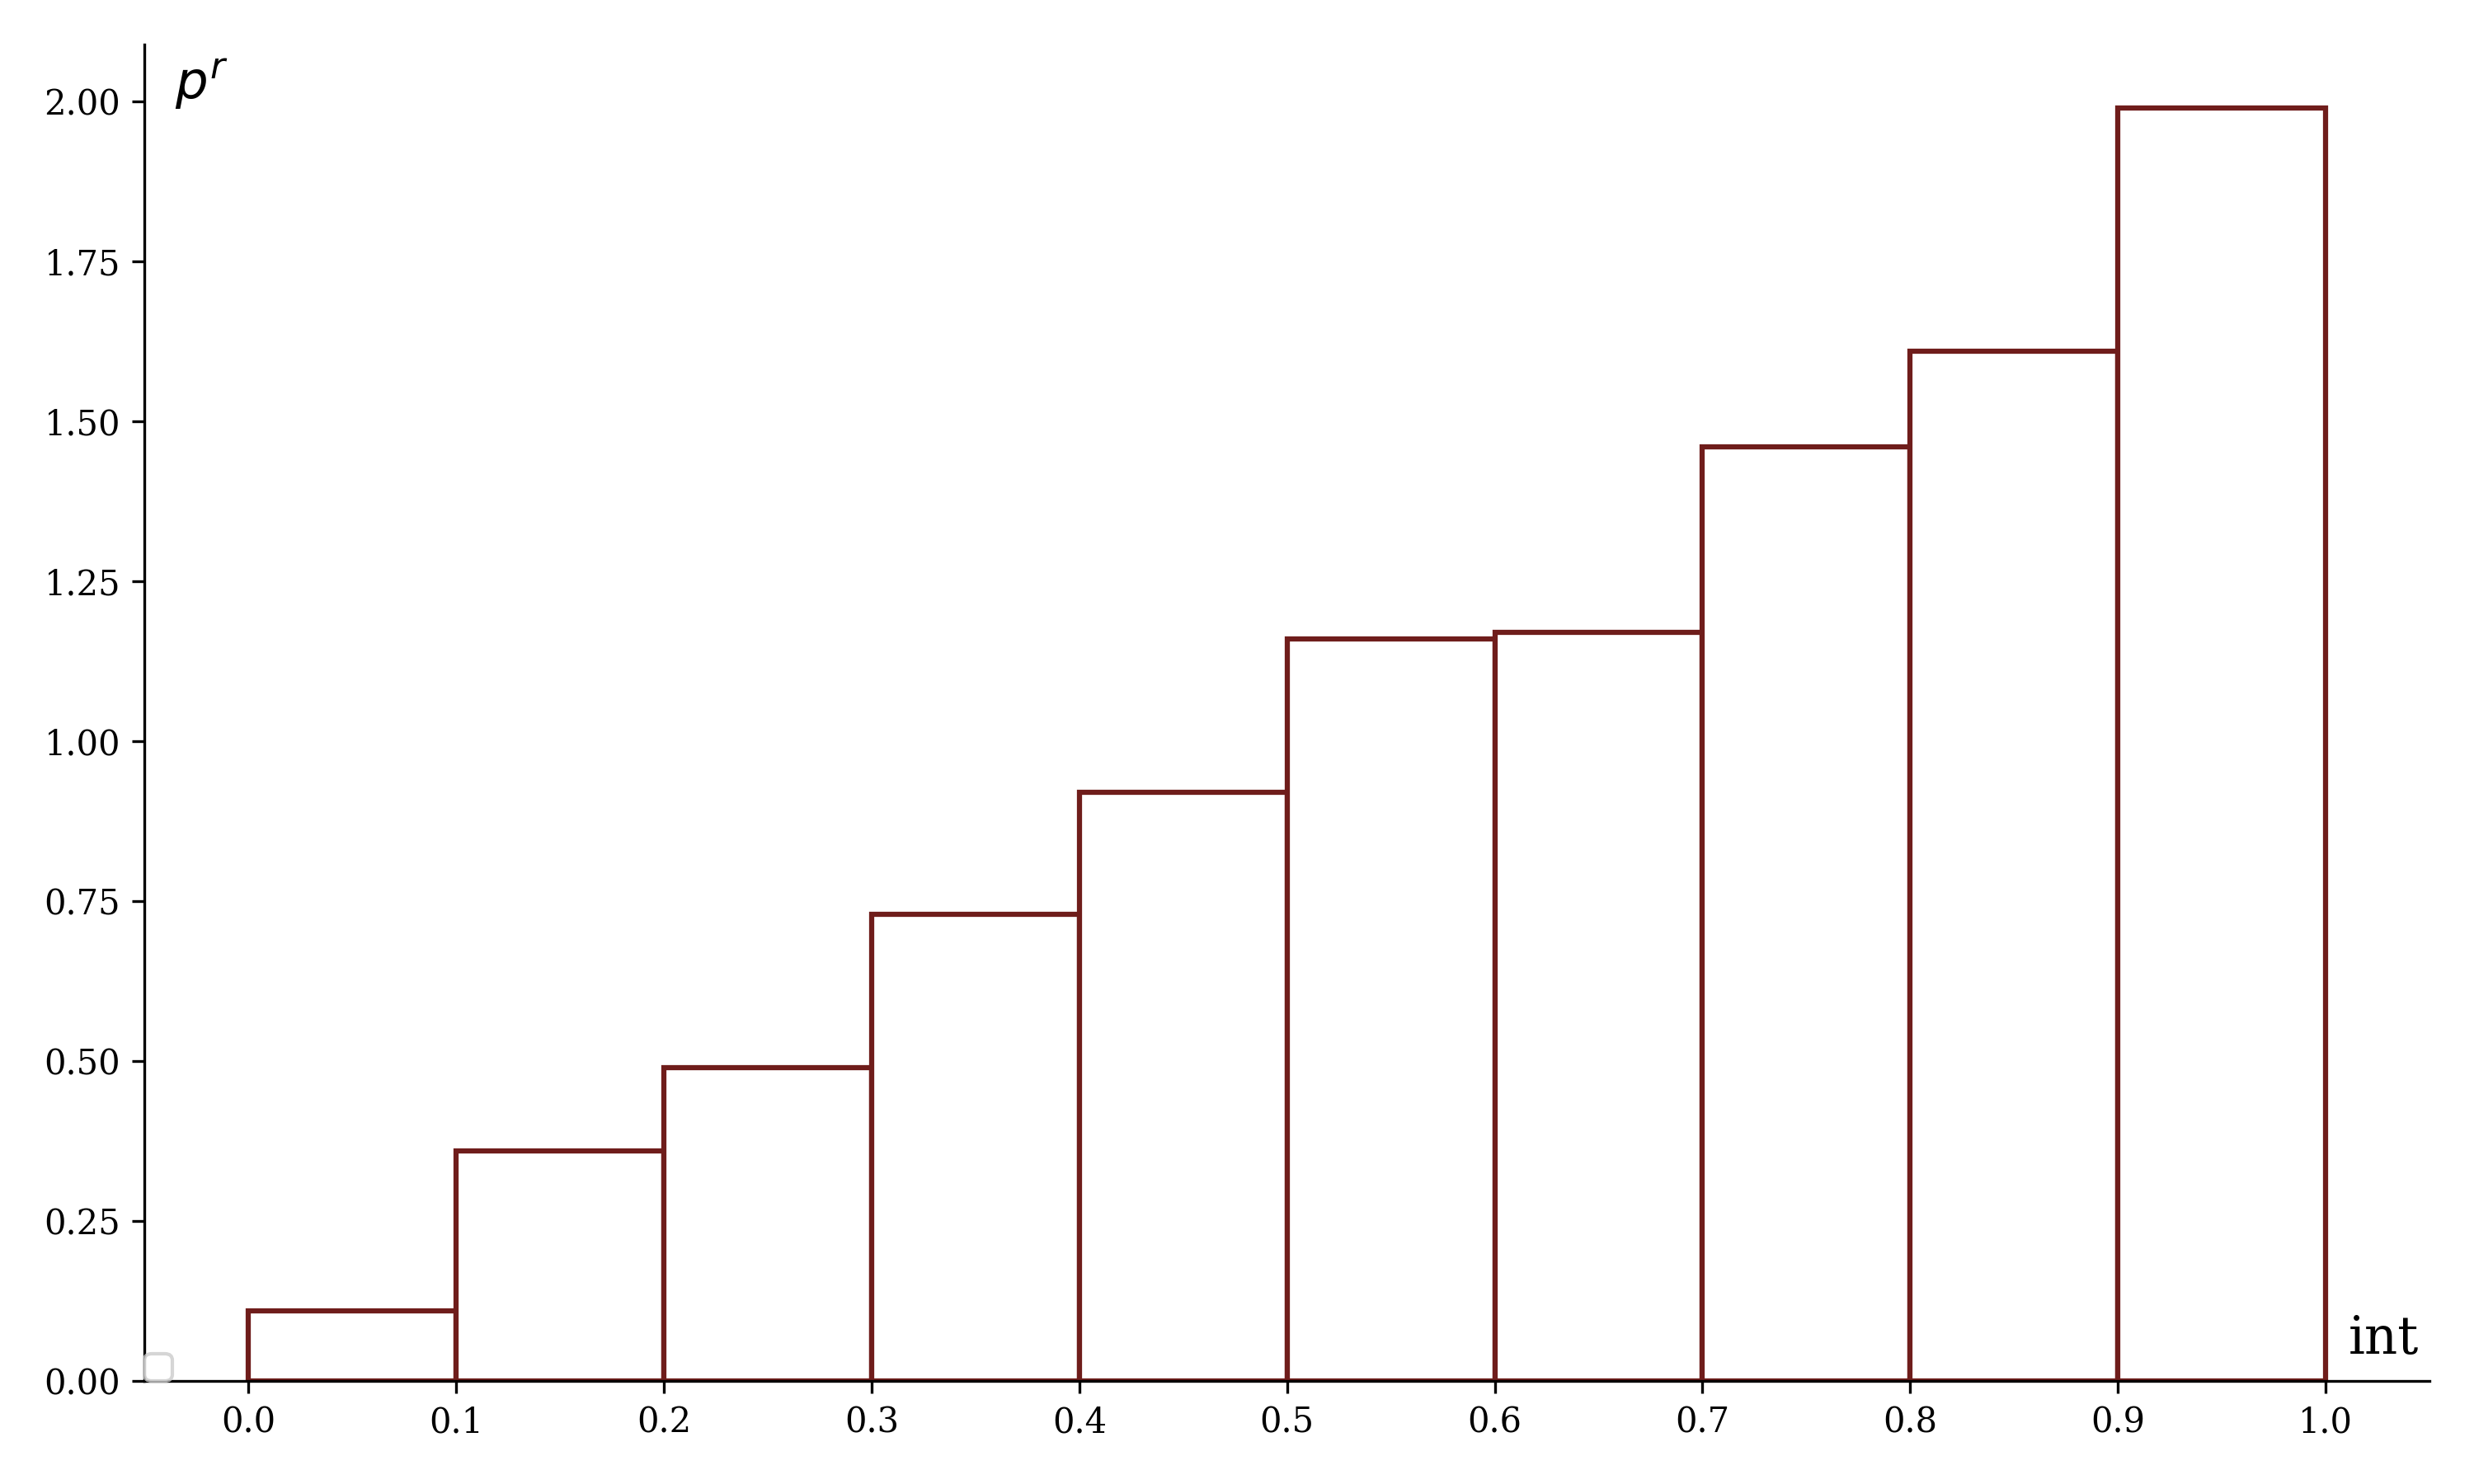
\includegraphics[width=\textwidth, height=\textheight, keepaspectratio]{test_sample_hist} \\
\end{center}

Посмотрим также гистограммы первых 36ти выборок после демонстрационной:

\newpage\newgeometry{margin=1cm, bottom=20mm}

\begin{minipage}[t]{0.25\textwidth}
  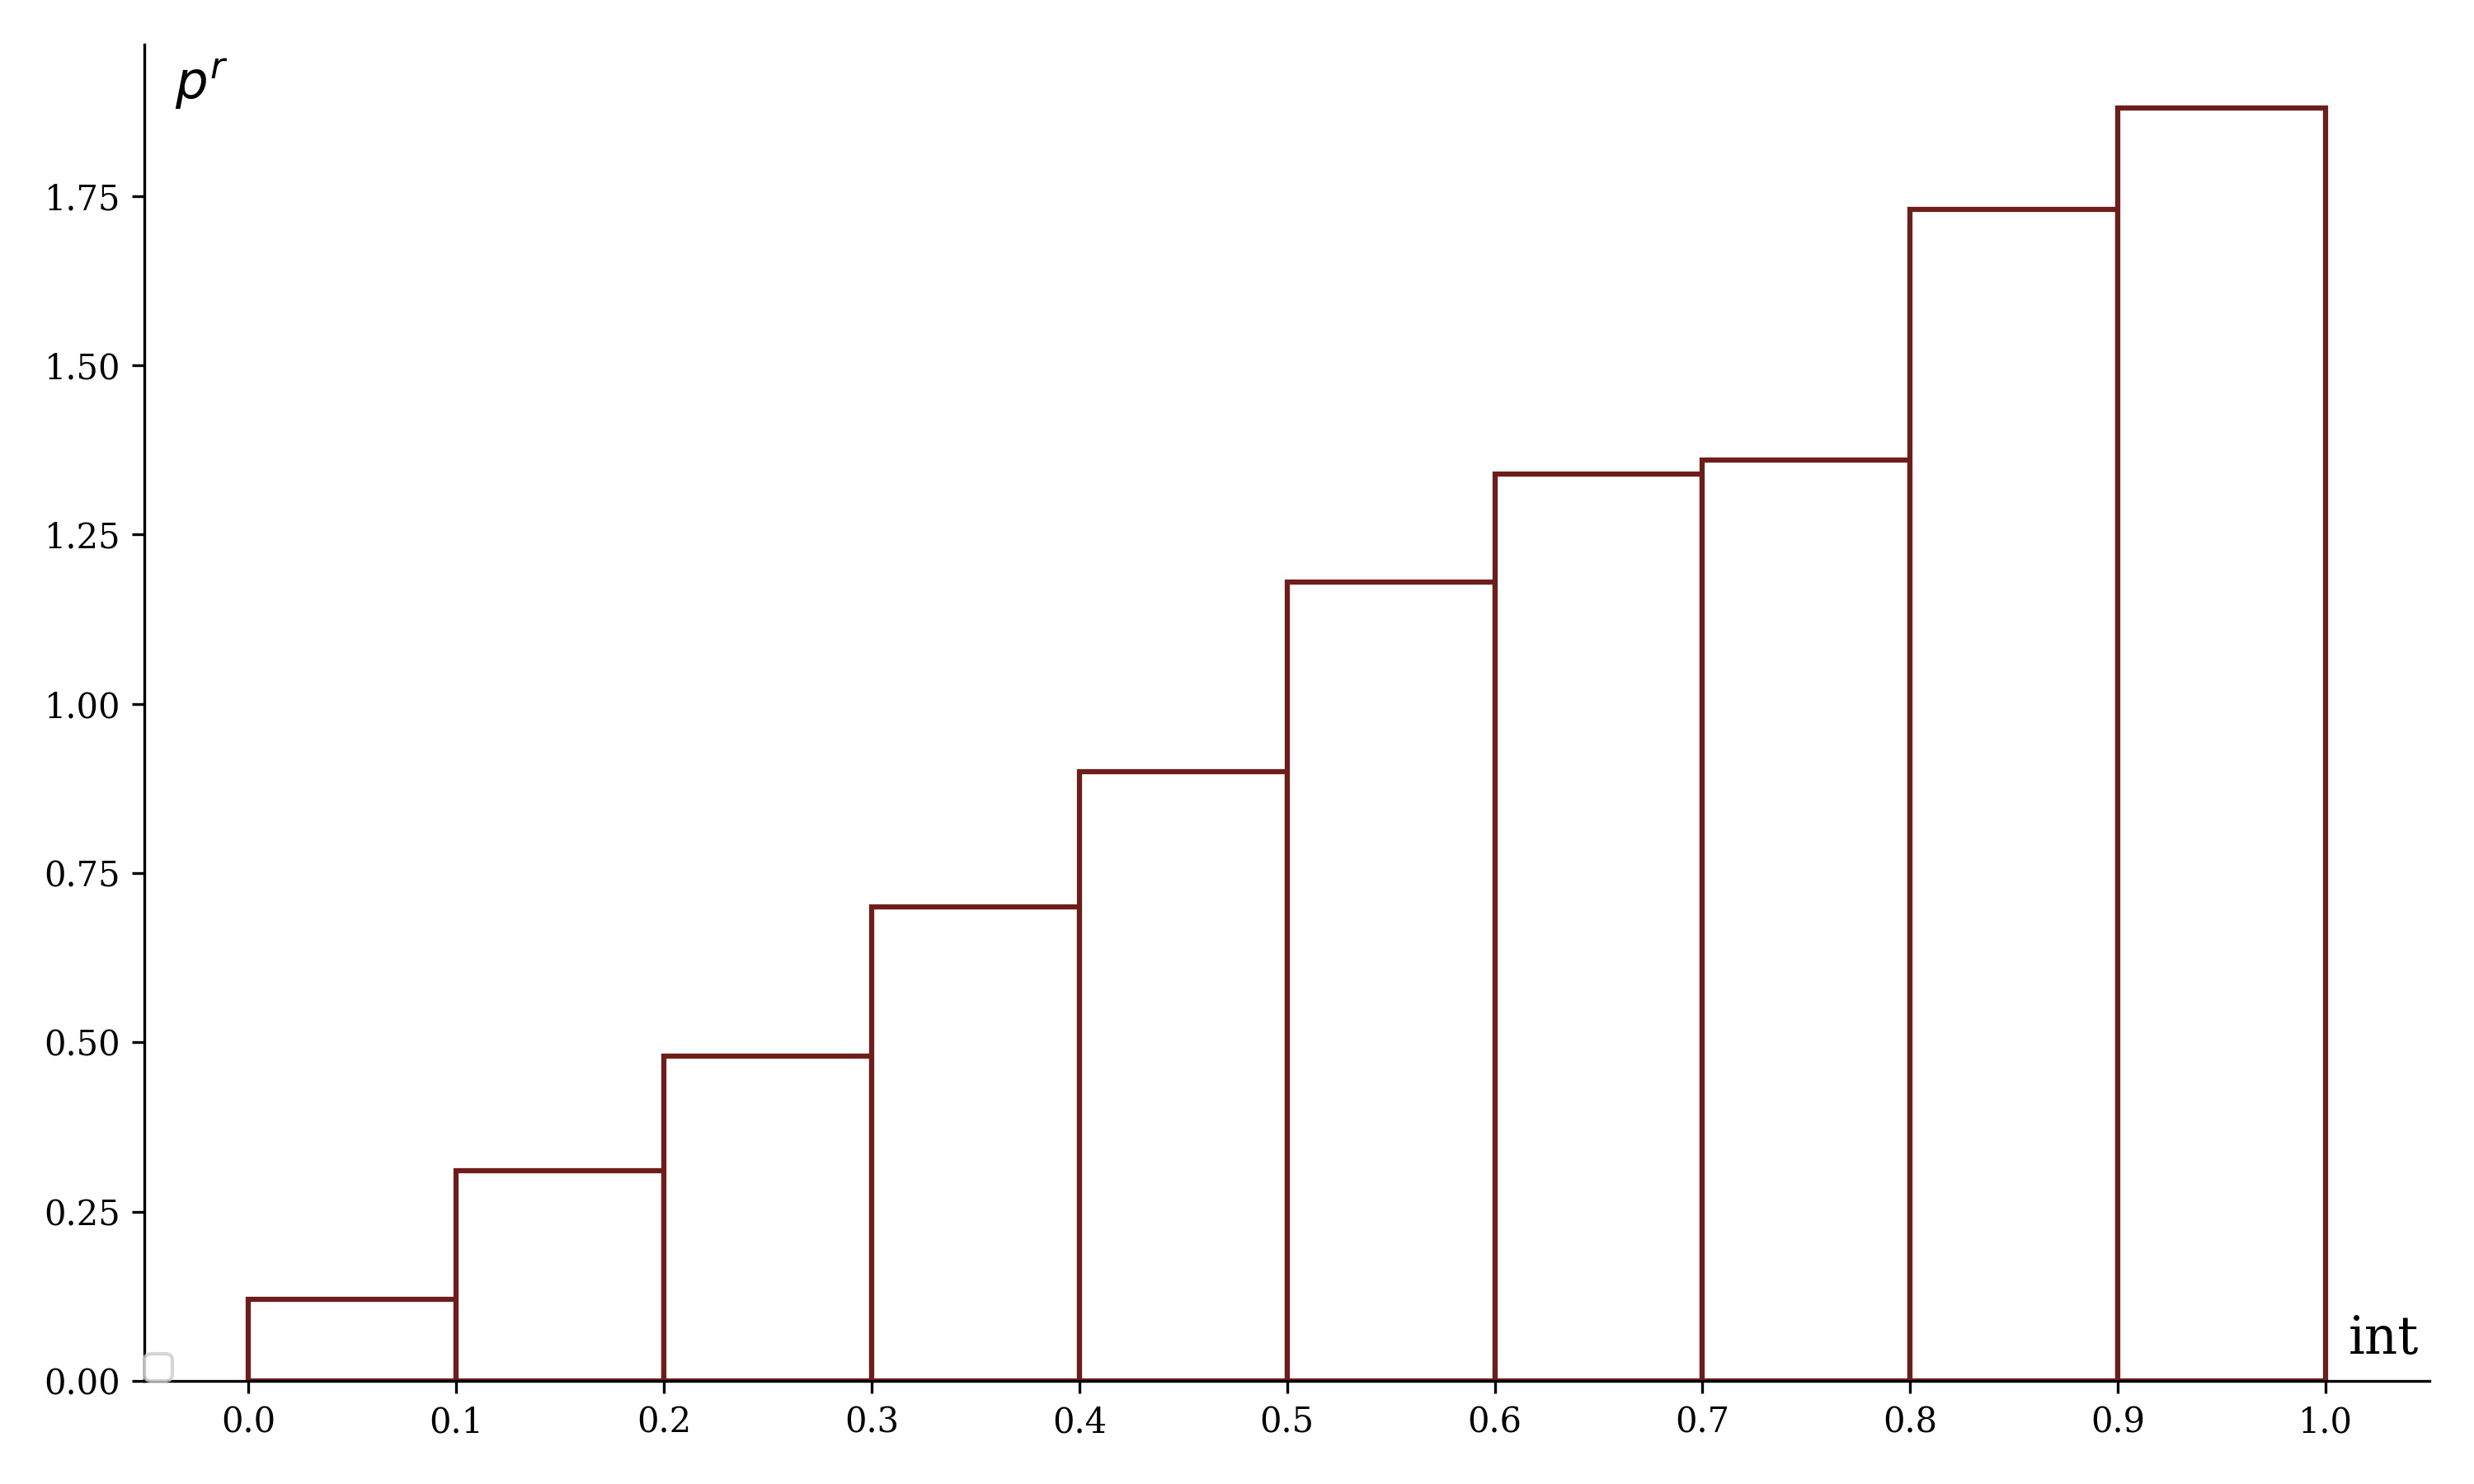
\includegraphics[width=\textwidth, height=\textheight, keepaspectratio]{sample1_hist}
\end{minipage}%
\begin{minipage}[t]{0.25\textwidth}
  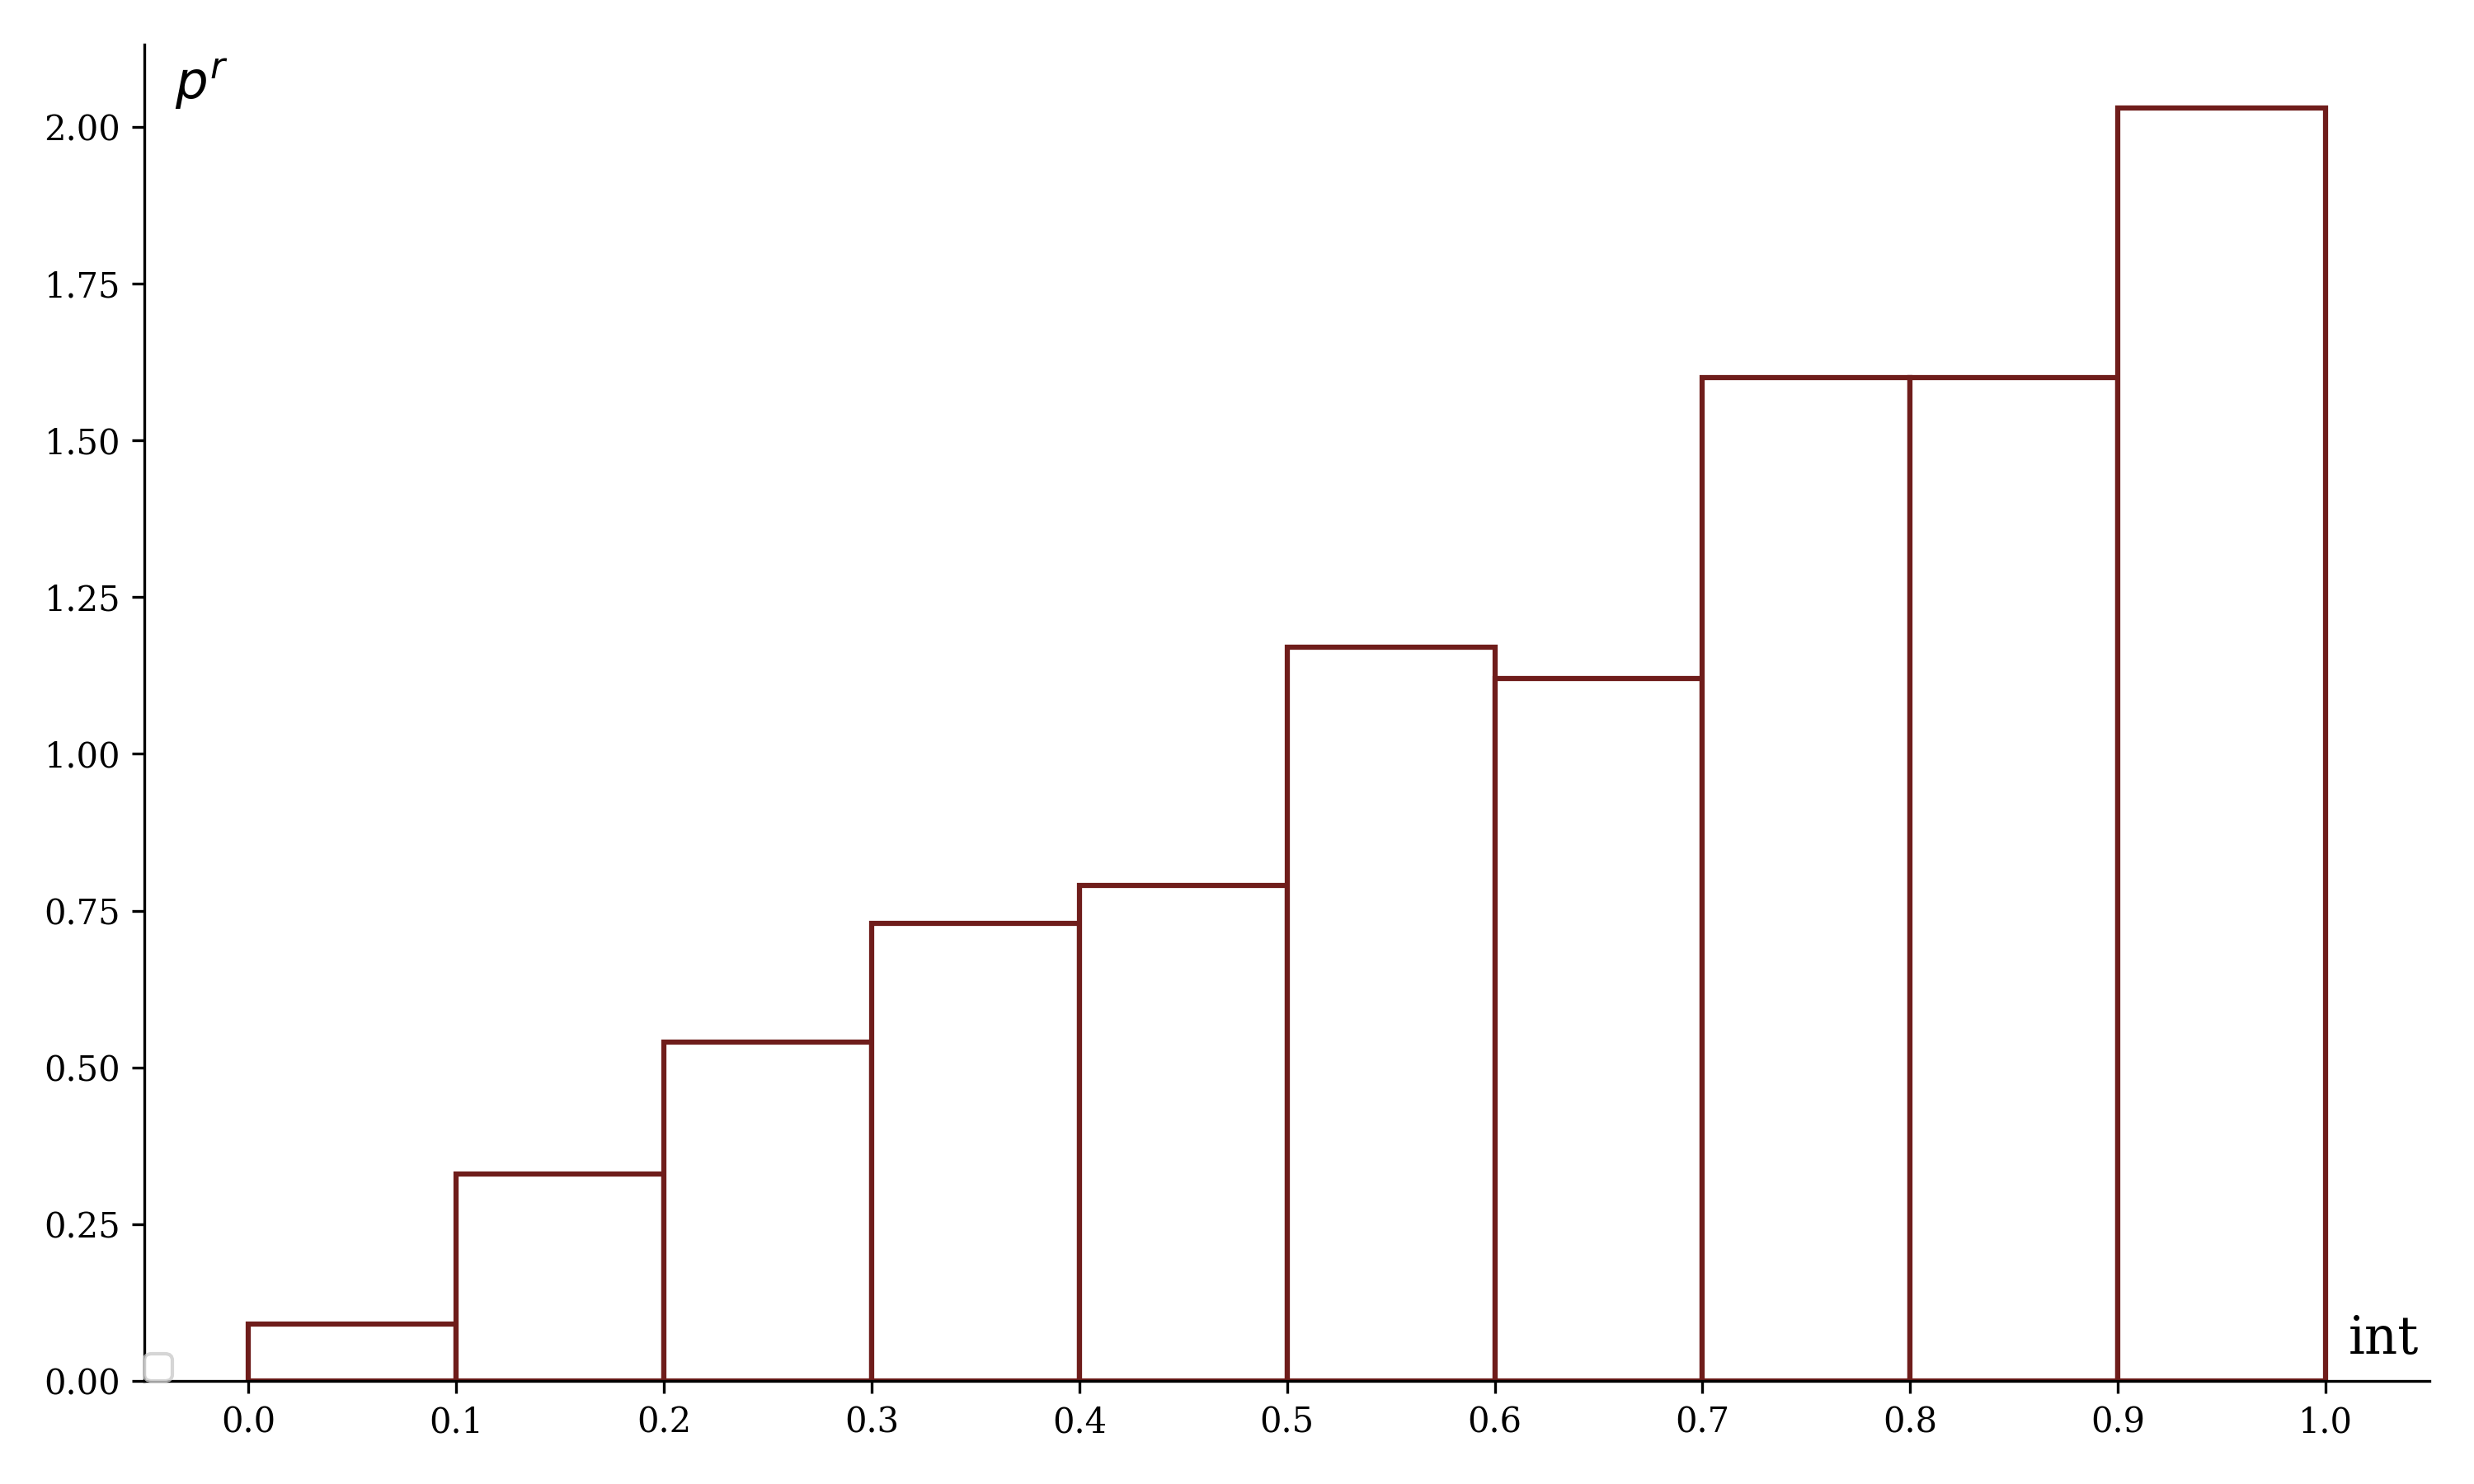
\includegraphics[width=\textwidth, height=\textheight, keepaspectratio]{sample2_hist}
\end{minipage}%
\begin{minipage}[t]{0.25\textwidth}
  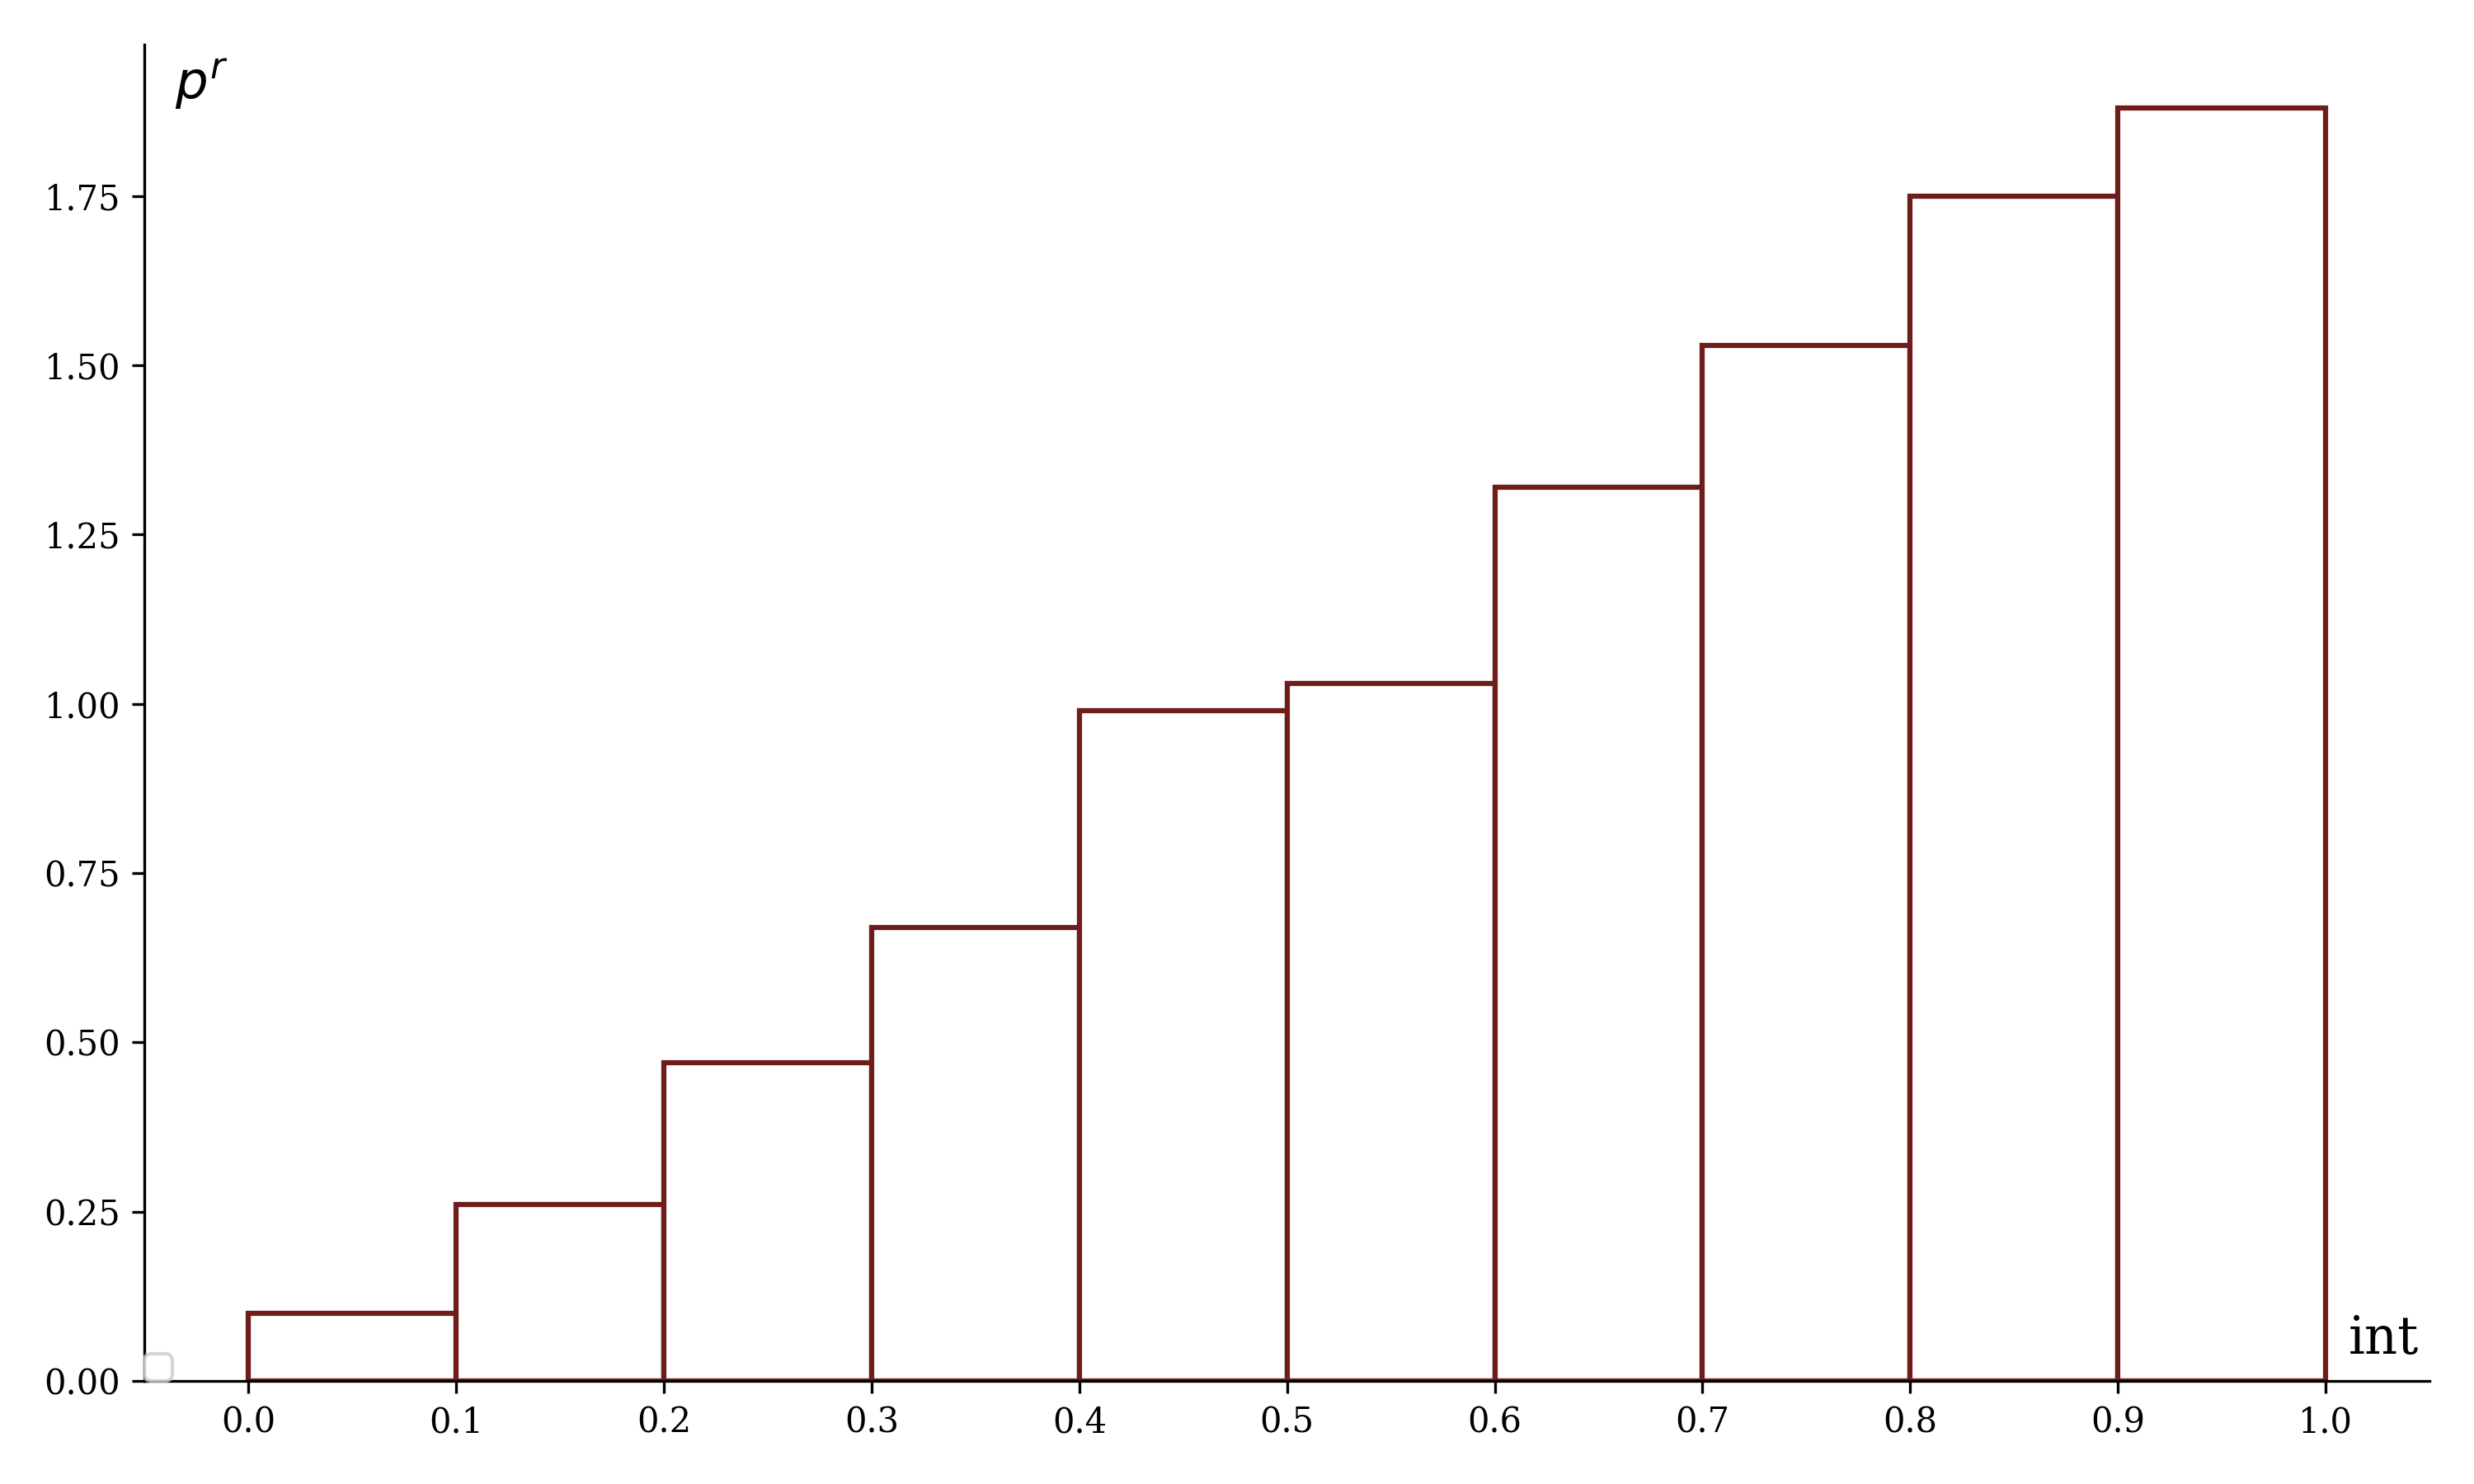
\includegraphics[width=\textwidth, height=\textheight, keepaspectratio]{sample3_hist}
\end{minipage}%
\begin{minipage}[t]{0.25\textwidth}
  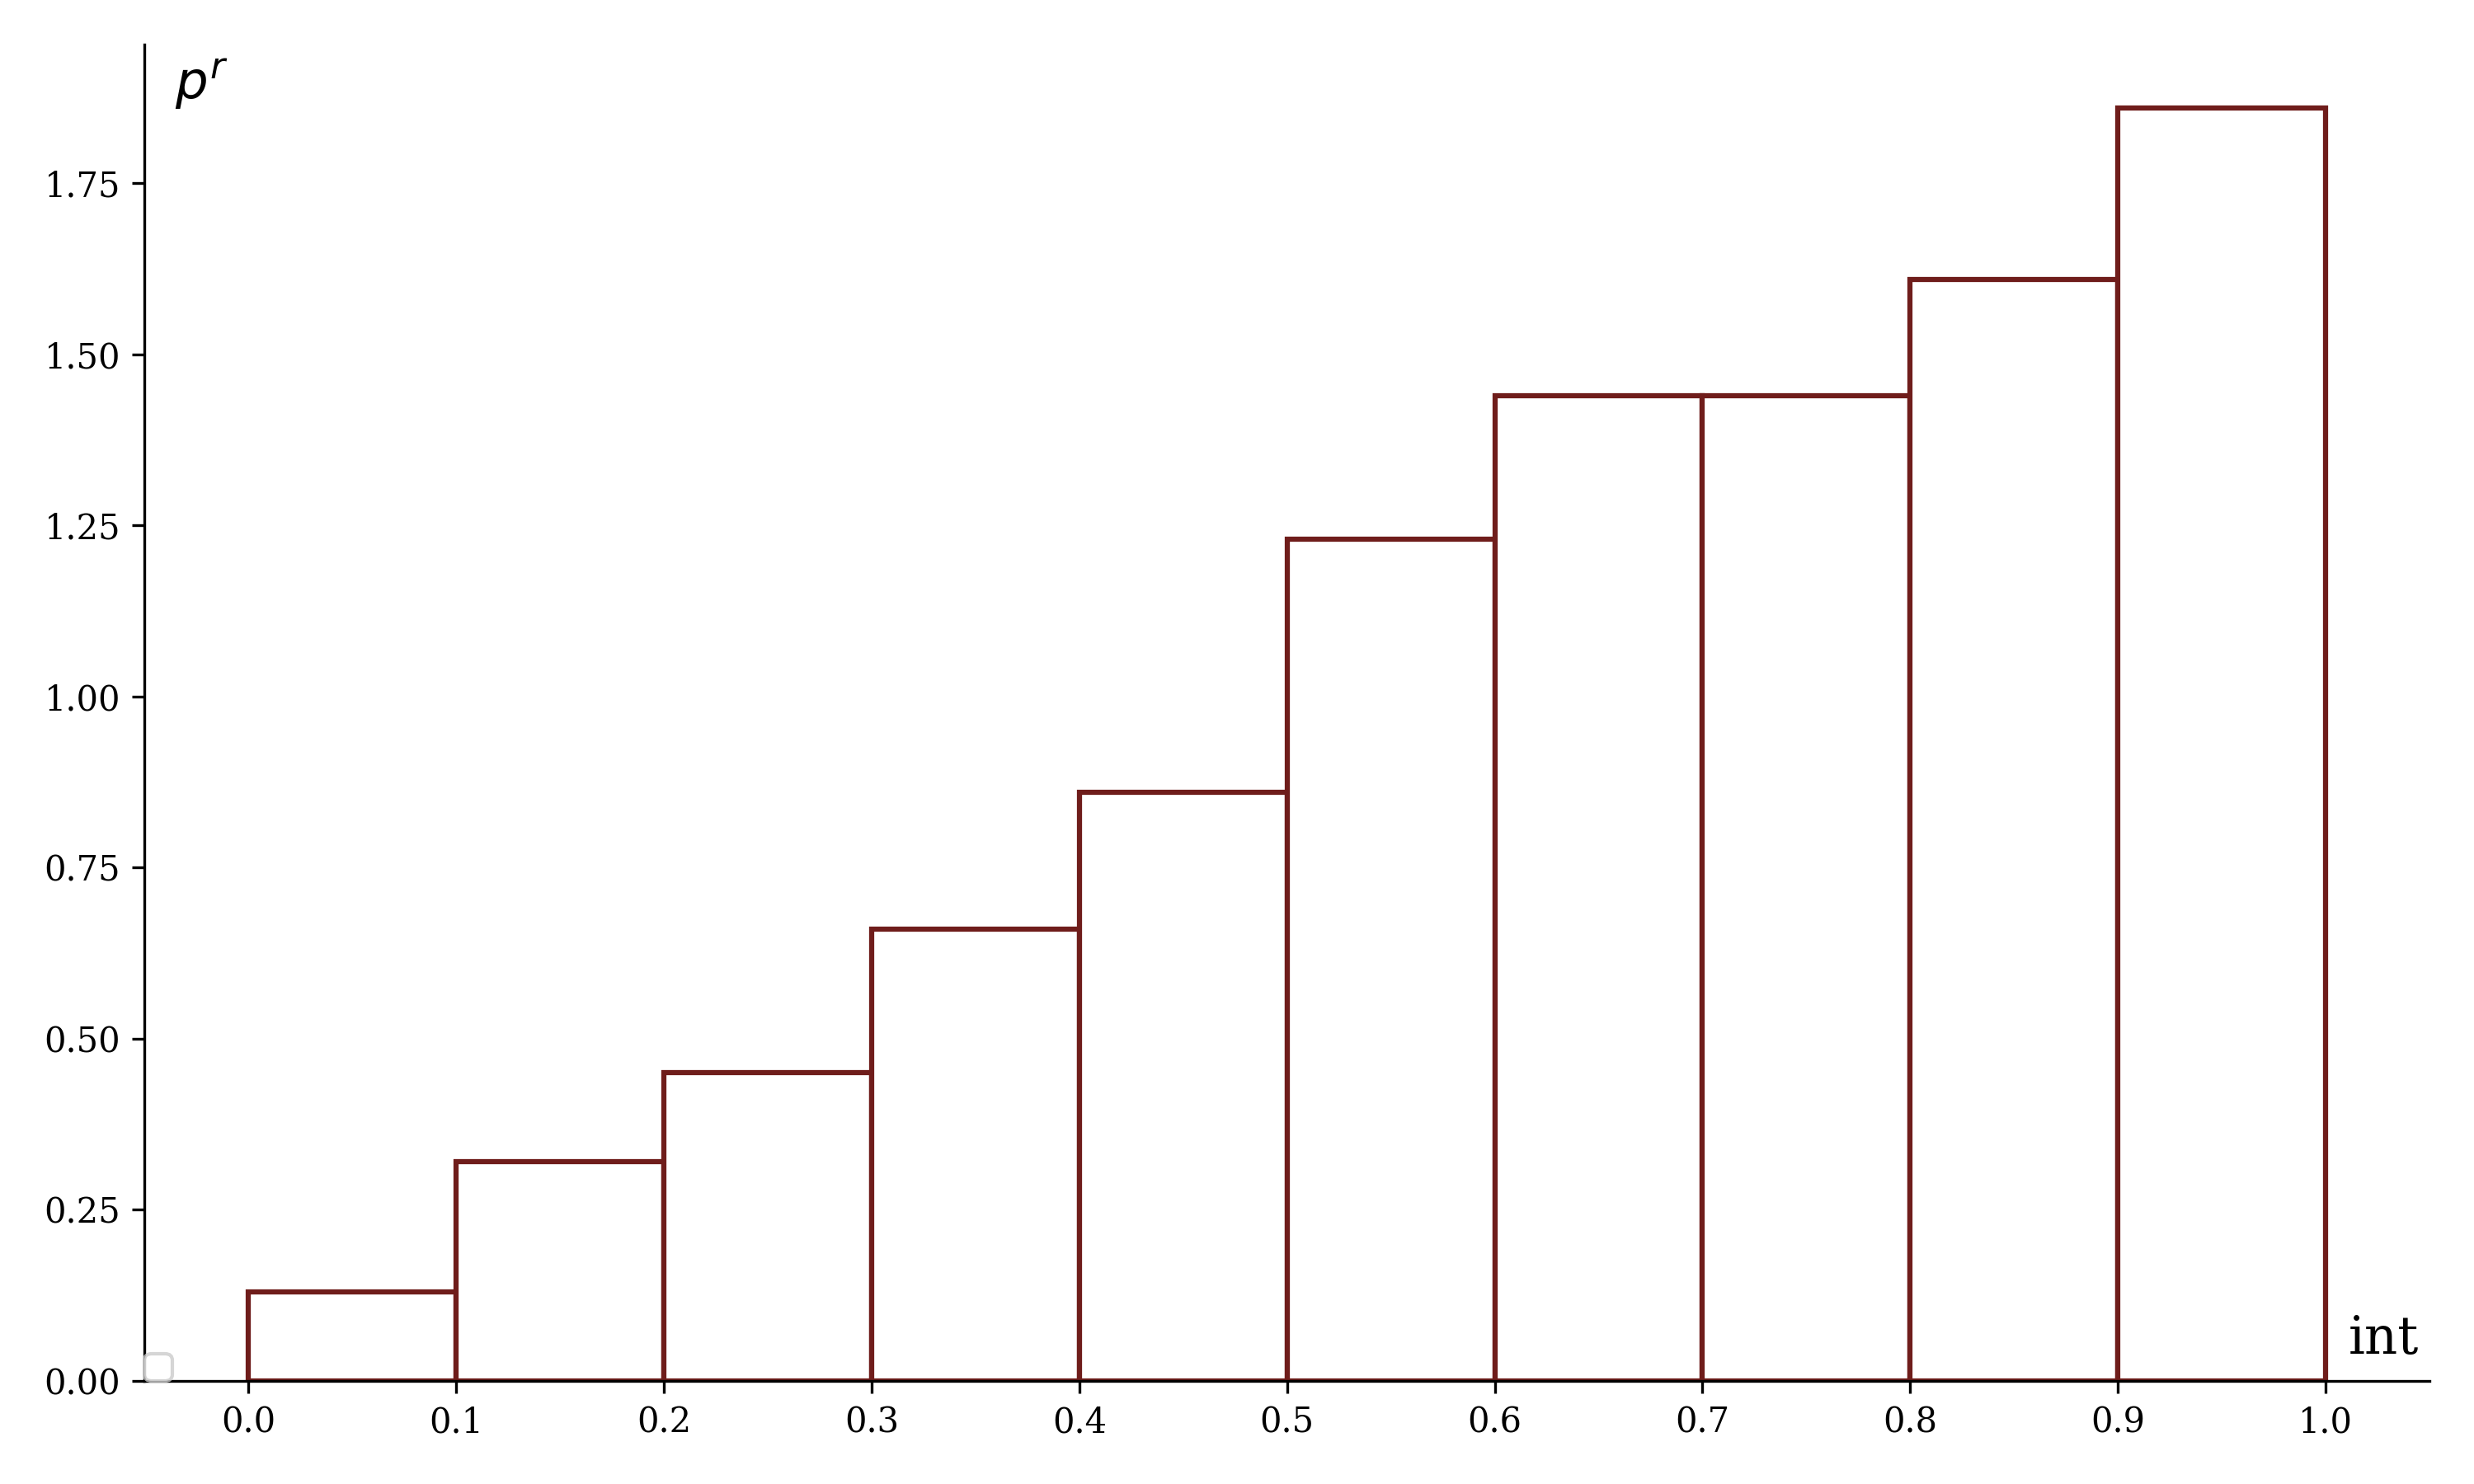
\includegraphics[width=\textwidth, height=\textheight, keepaspectratio]{sample4_hist}
\end{minipage}

\begin{minipage}[t]{0.25\textwidth}
  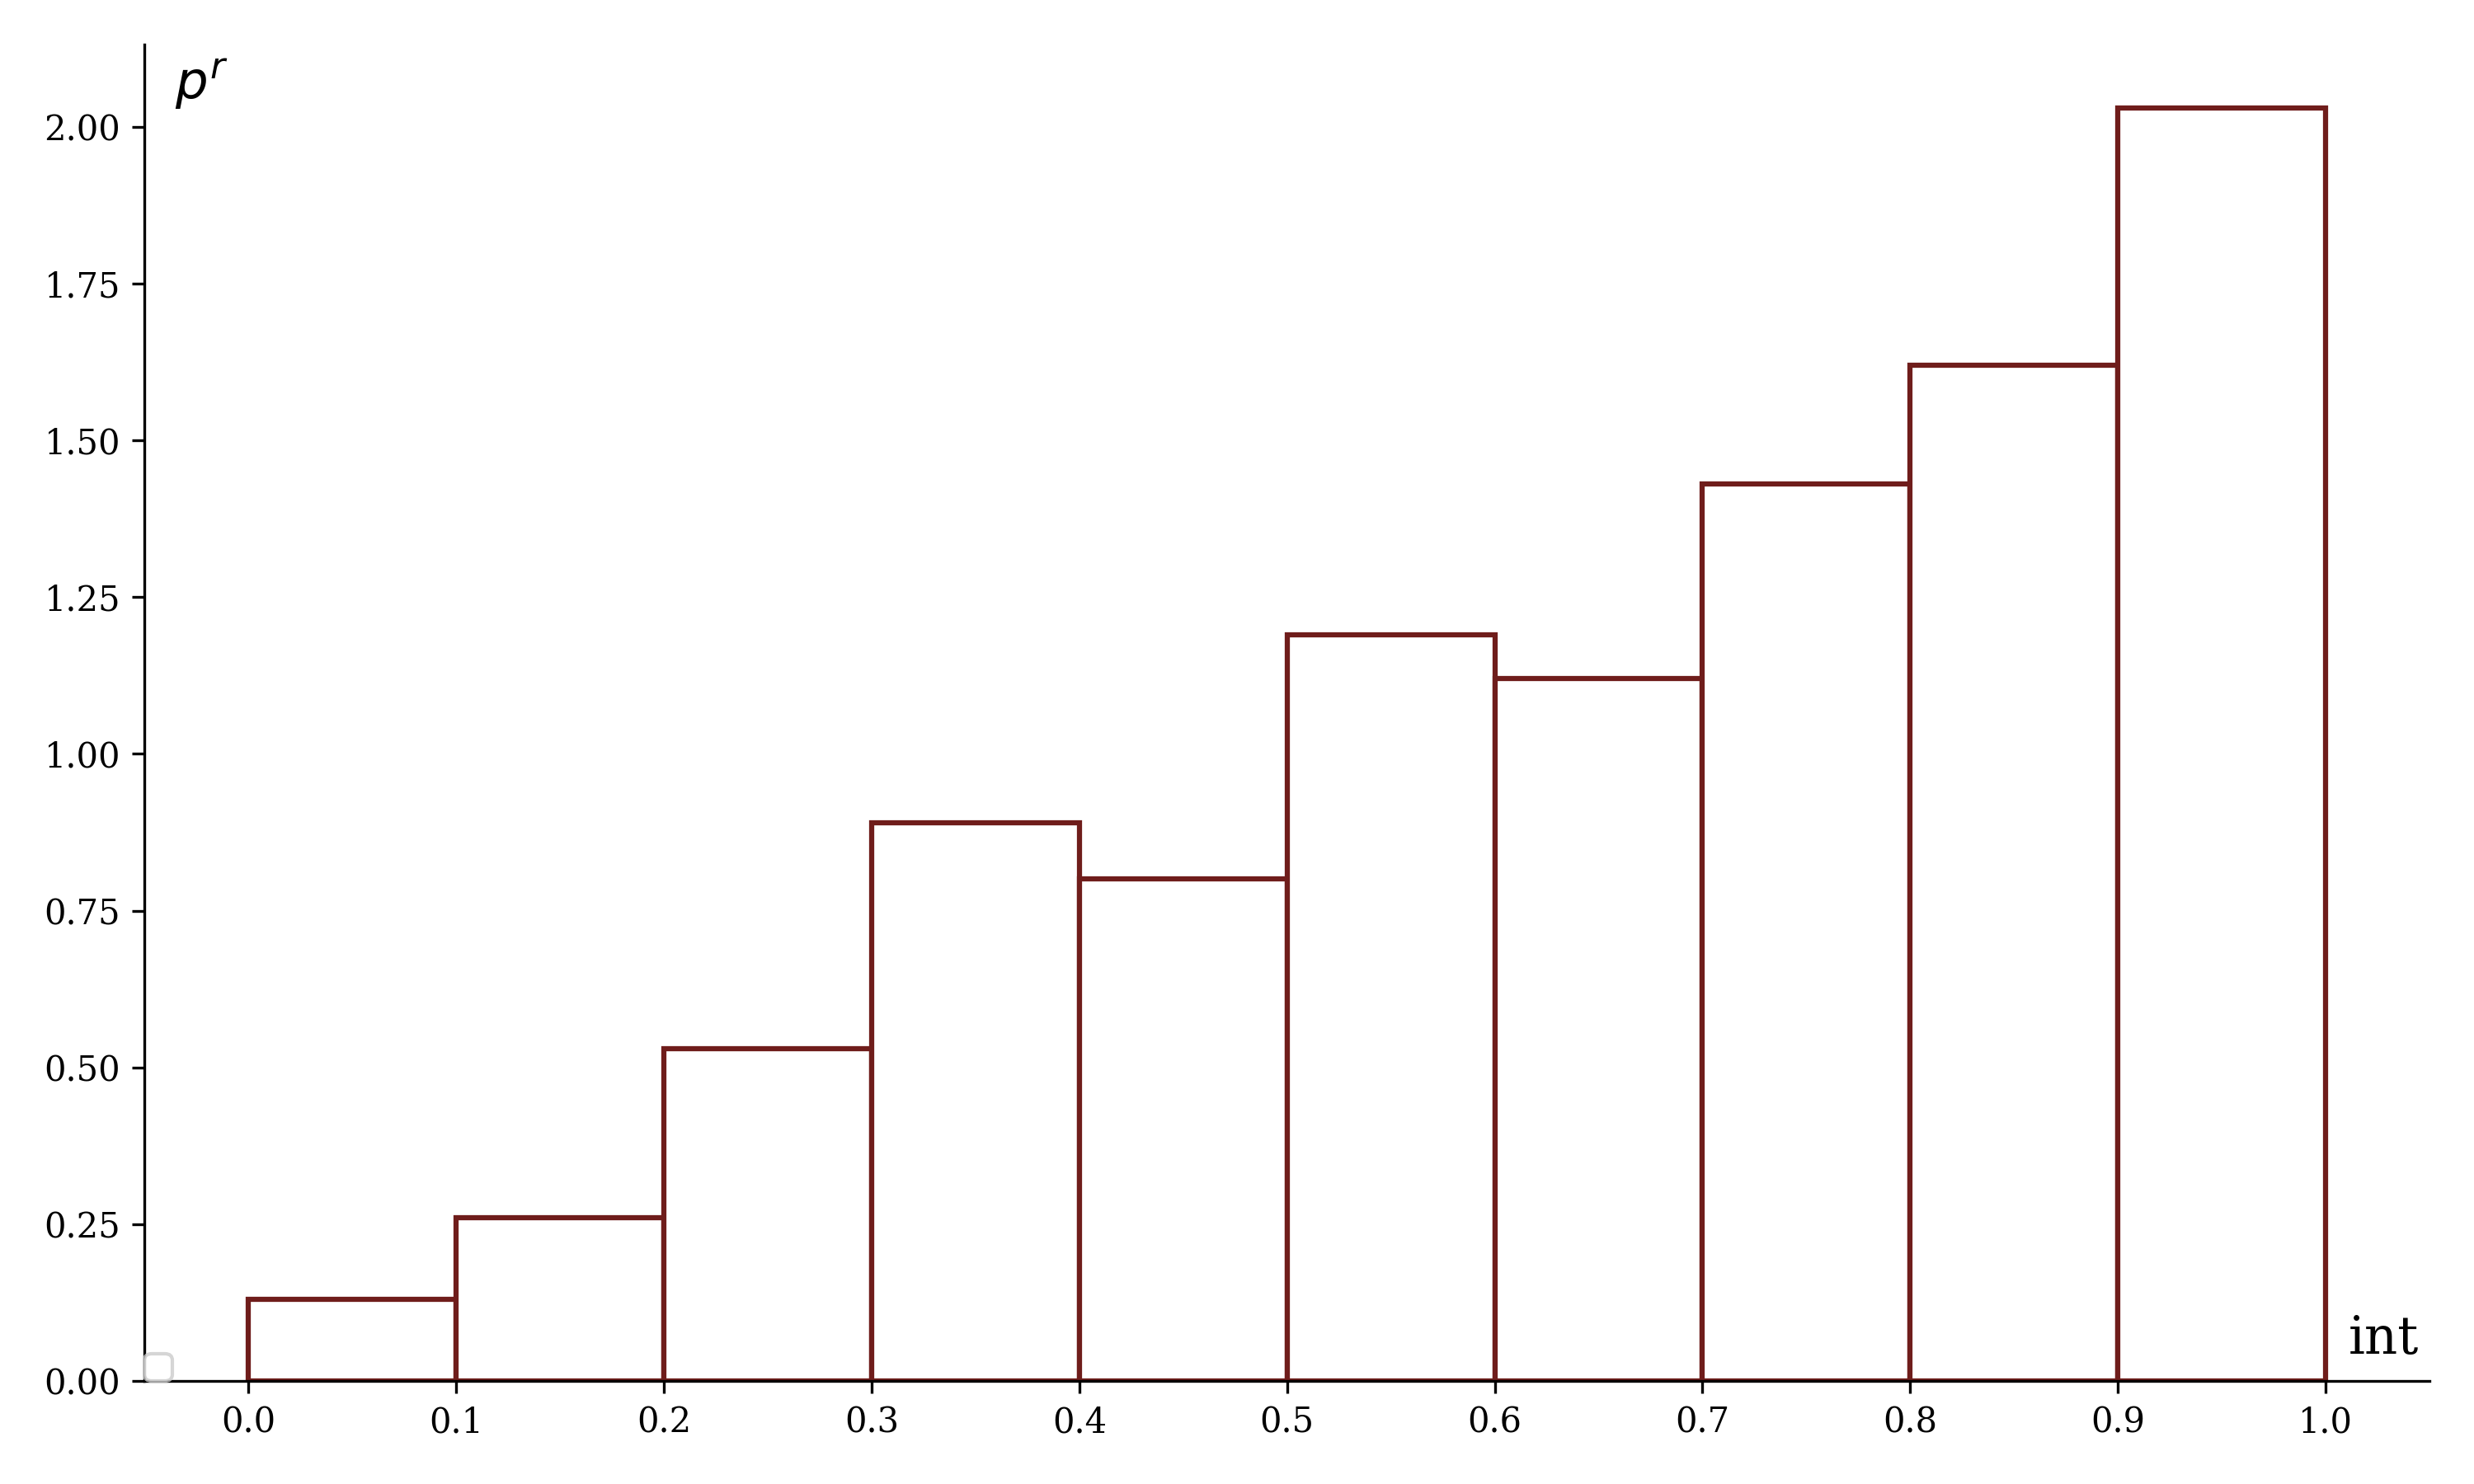
\includegraphics[width=\textwidth, height=\textheight, keepaspectratio]{sample5_hist}
\end{minipage}%
\begin{minipage}[t]{0.25\textwidth}
  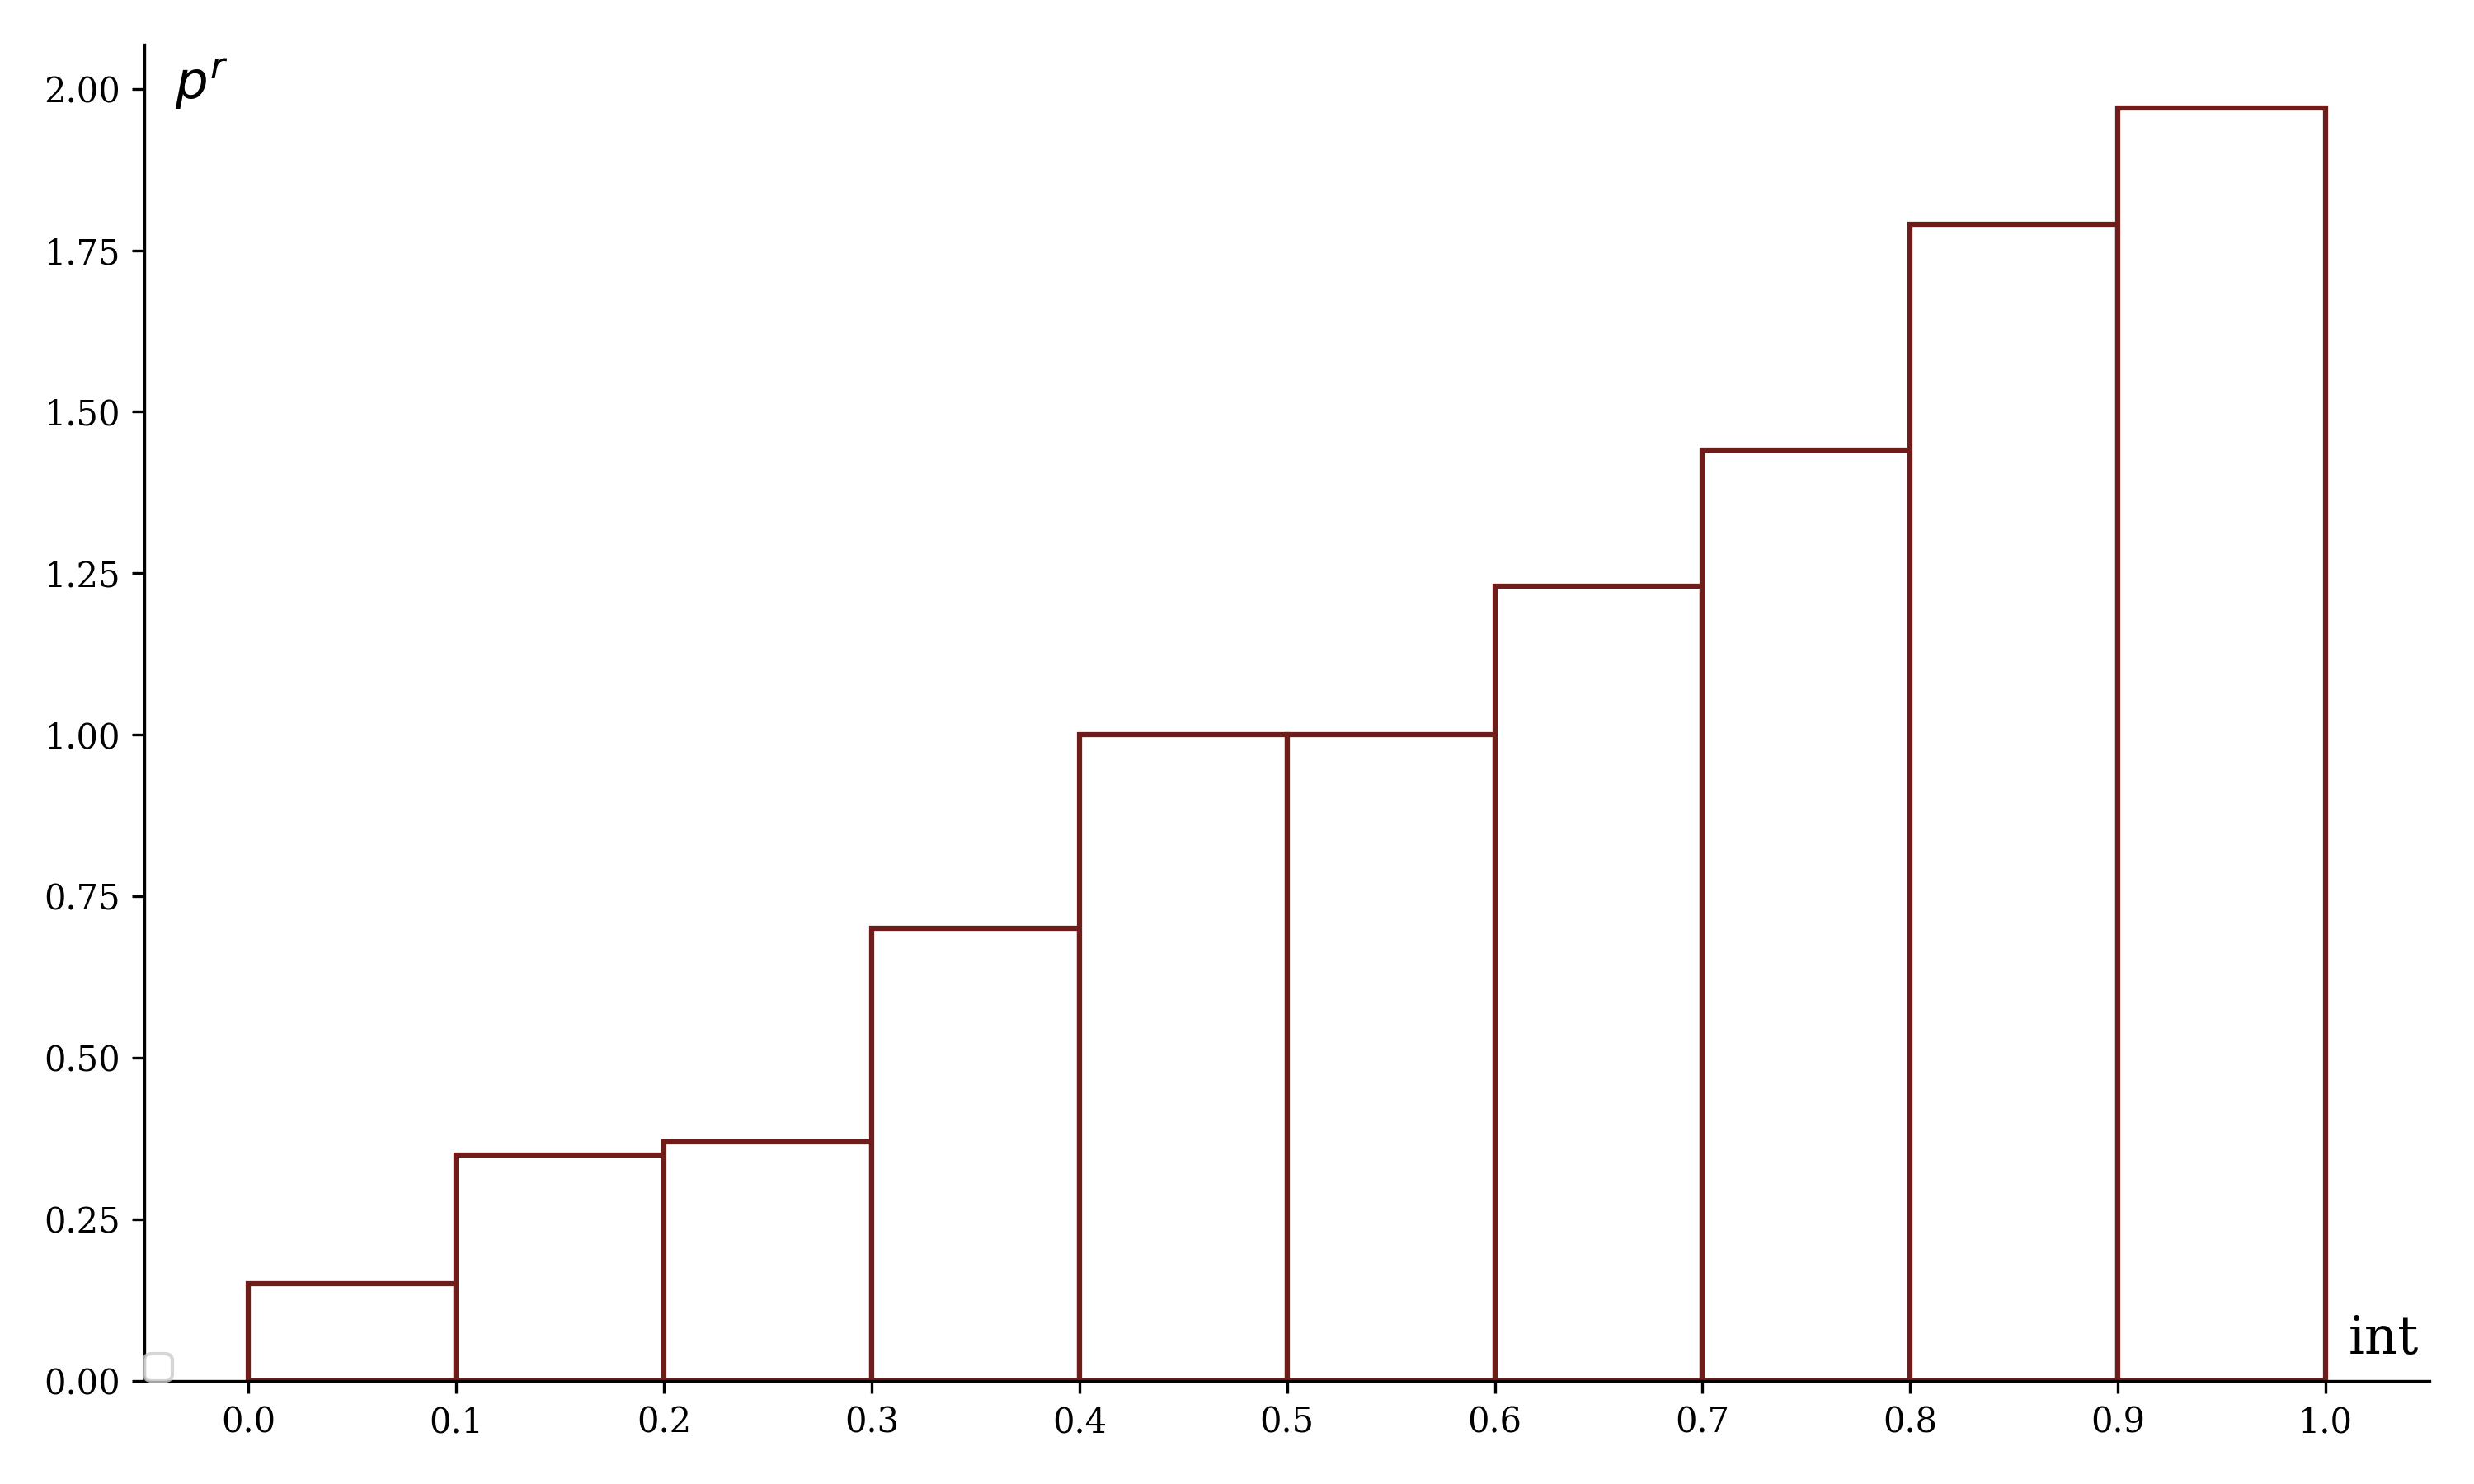
\includegraphics[width=\textwidth, height=\textheight, keepaspectratio]{sample6_hist}
\end{minipage}%
\begin{minipage}[t]{0.25\textwidth}
  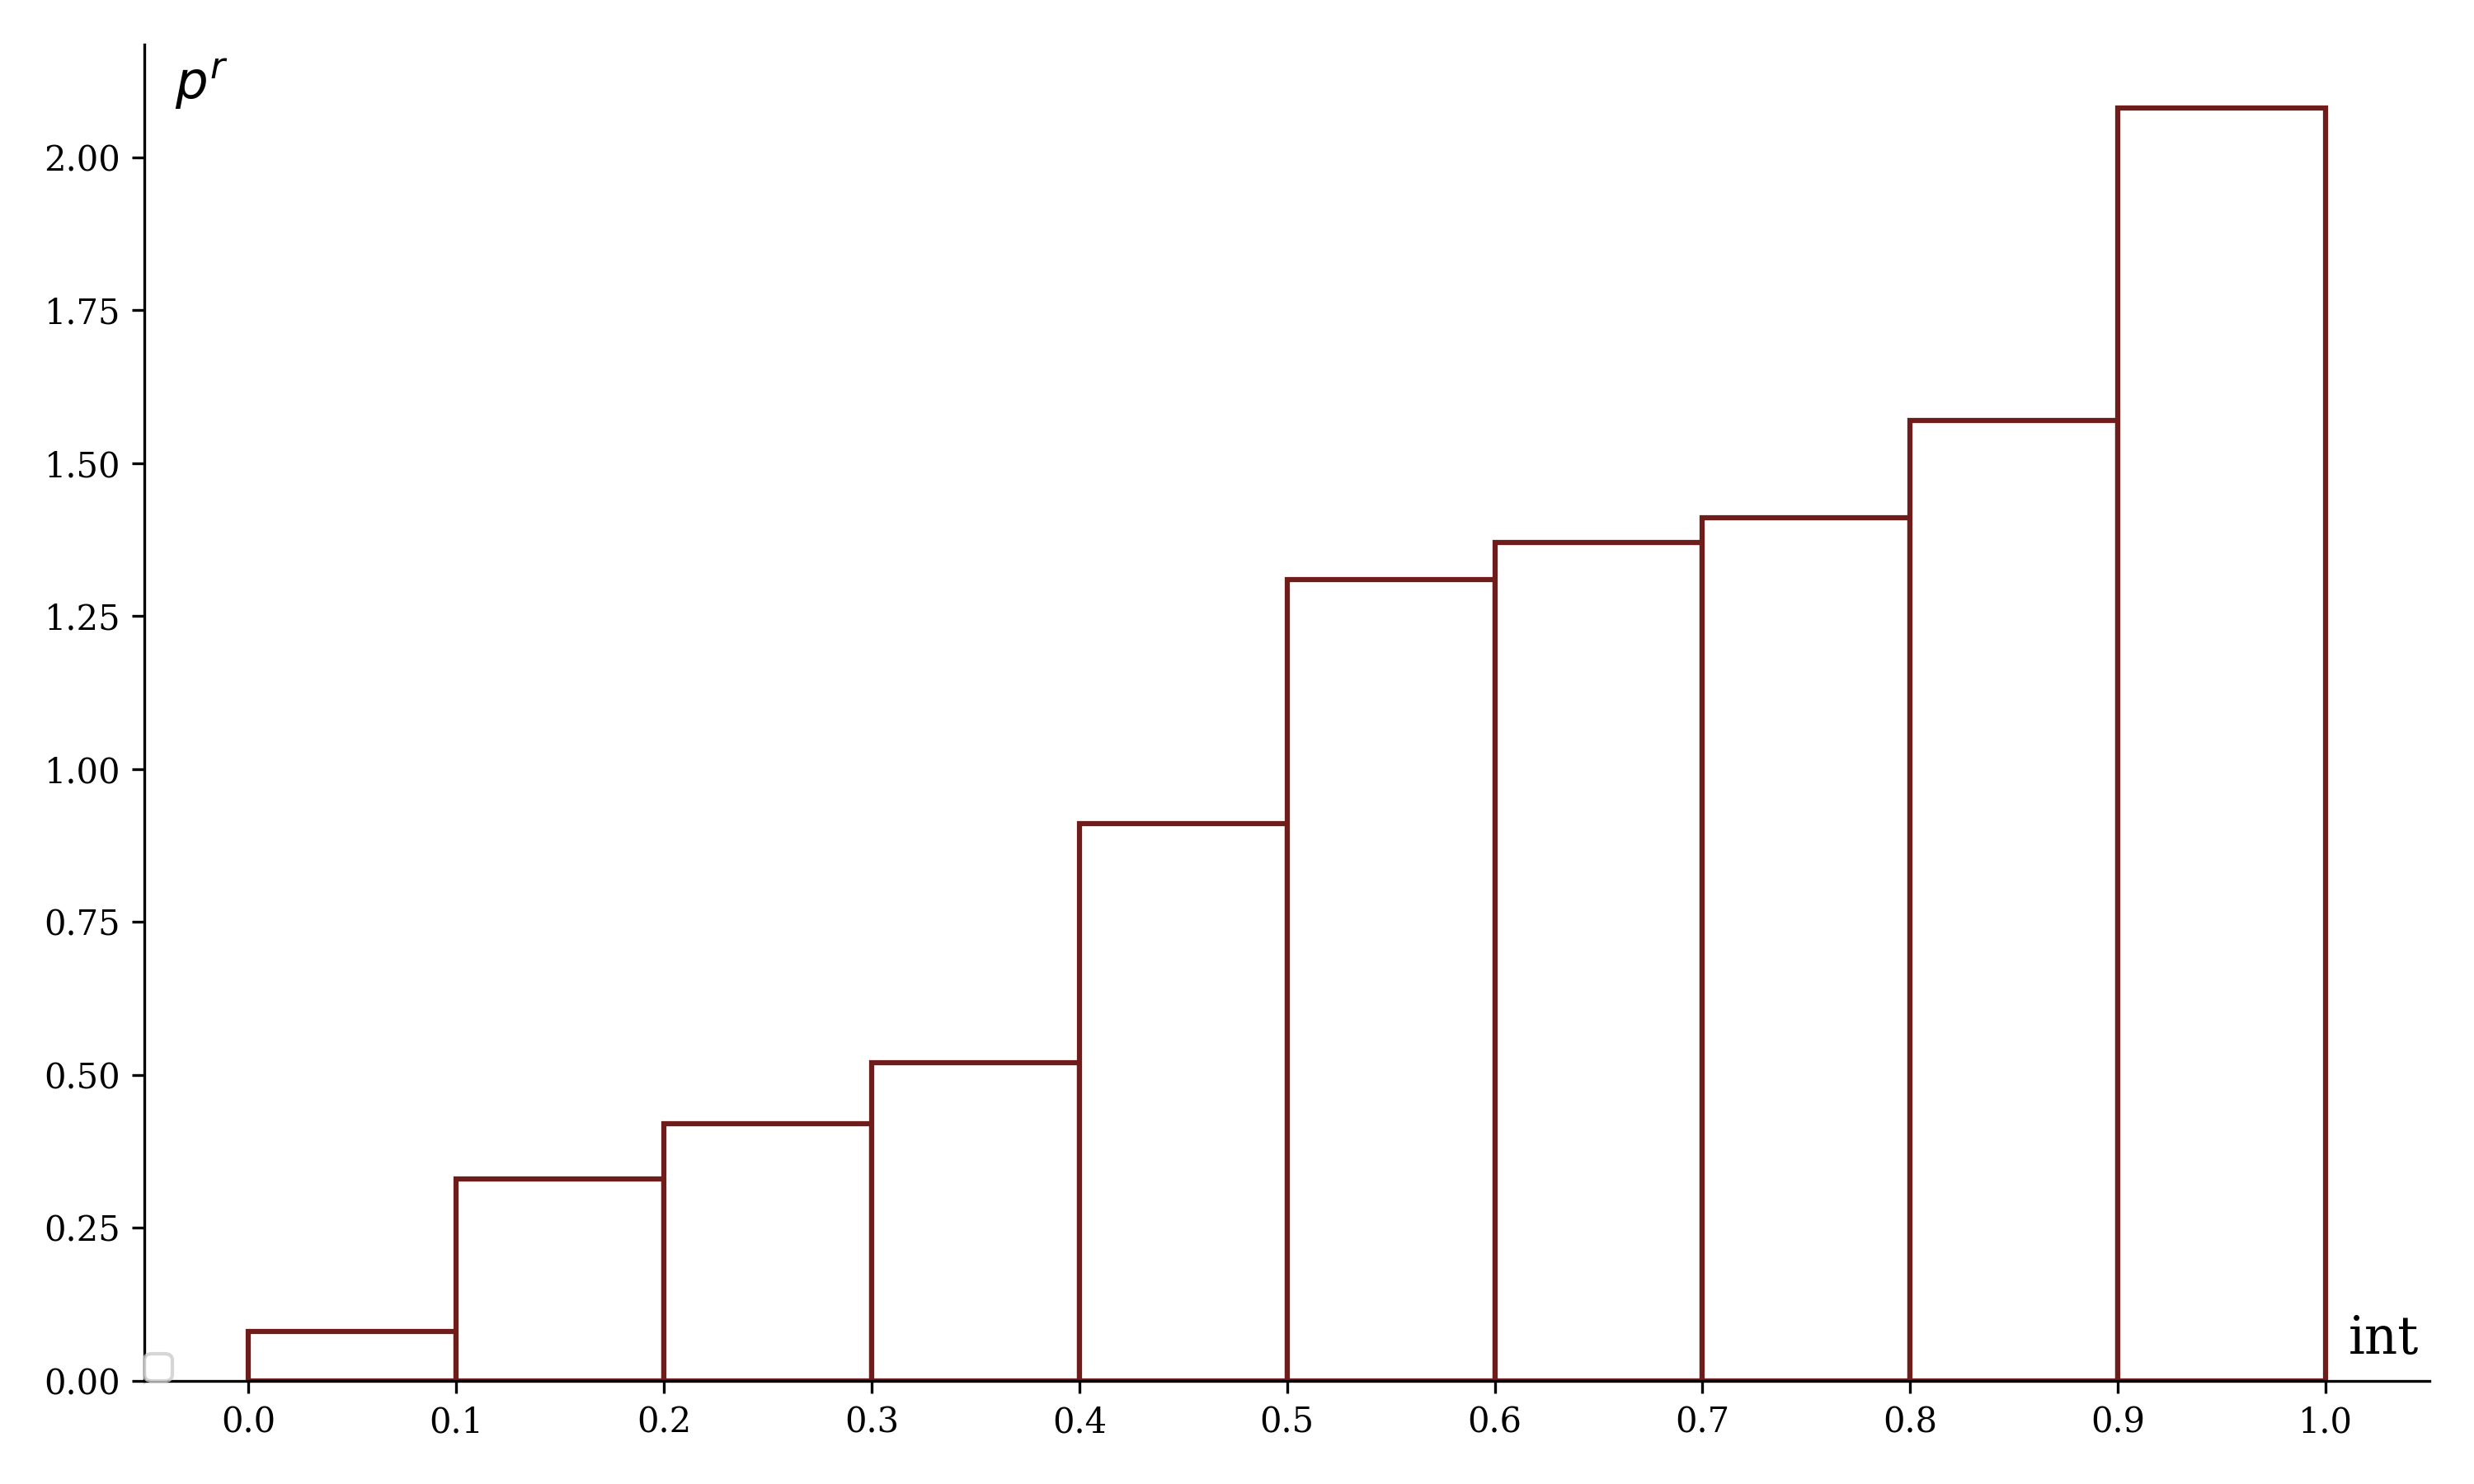
\includegraphics[width=\textwidth, height=\textheight, keepaspectratio]{sample7_hist}
\end{minipage}%
\begin{minipage}[t]{0.25\textwidth}
  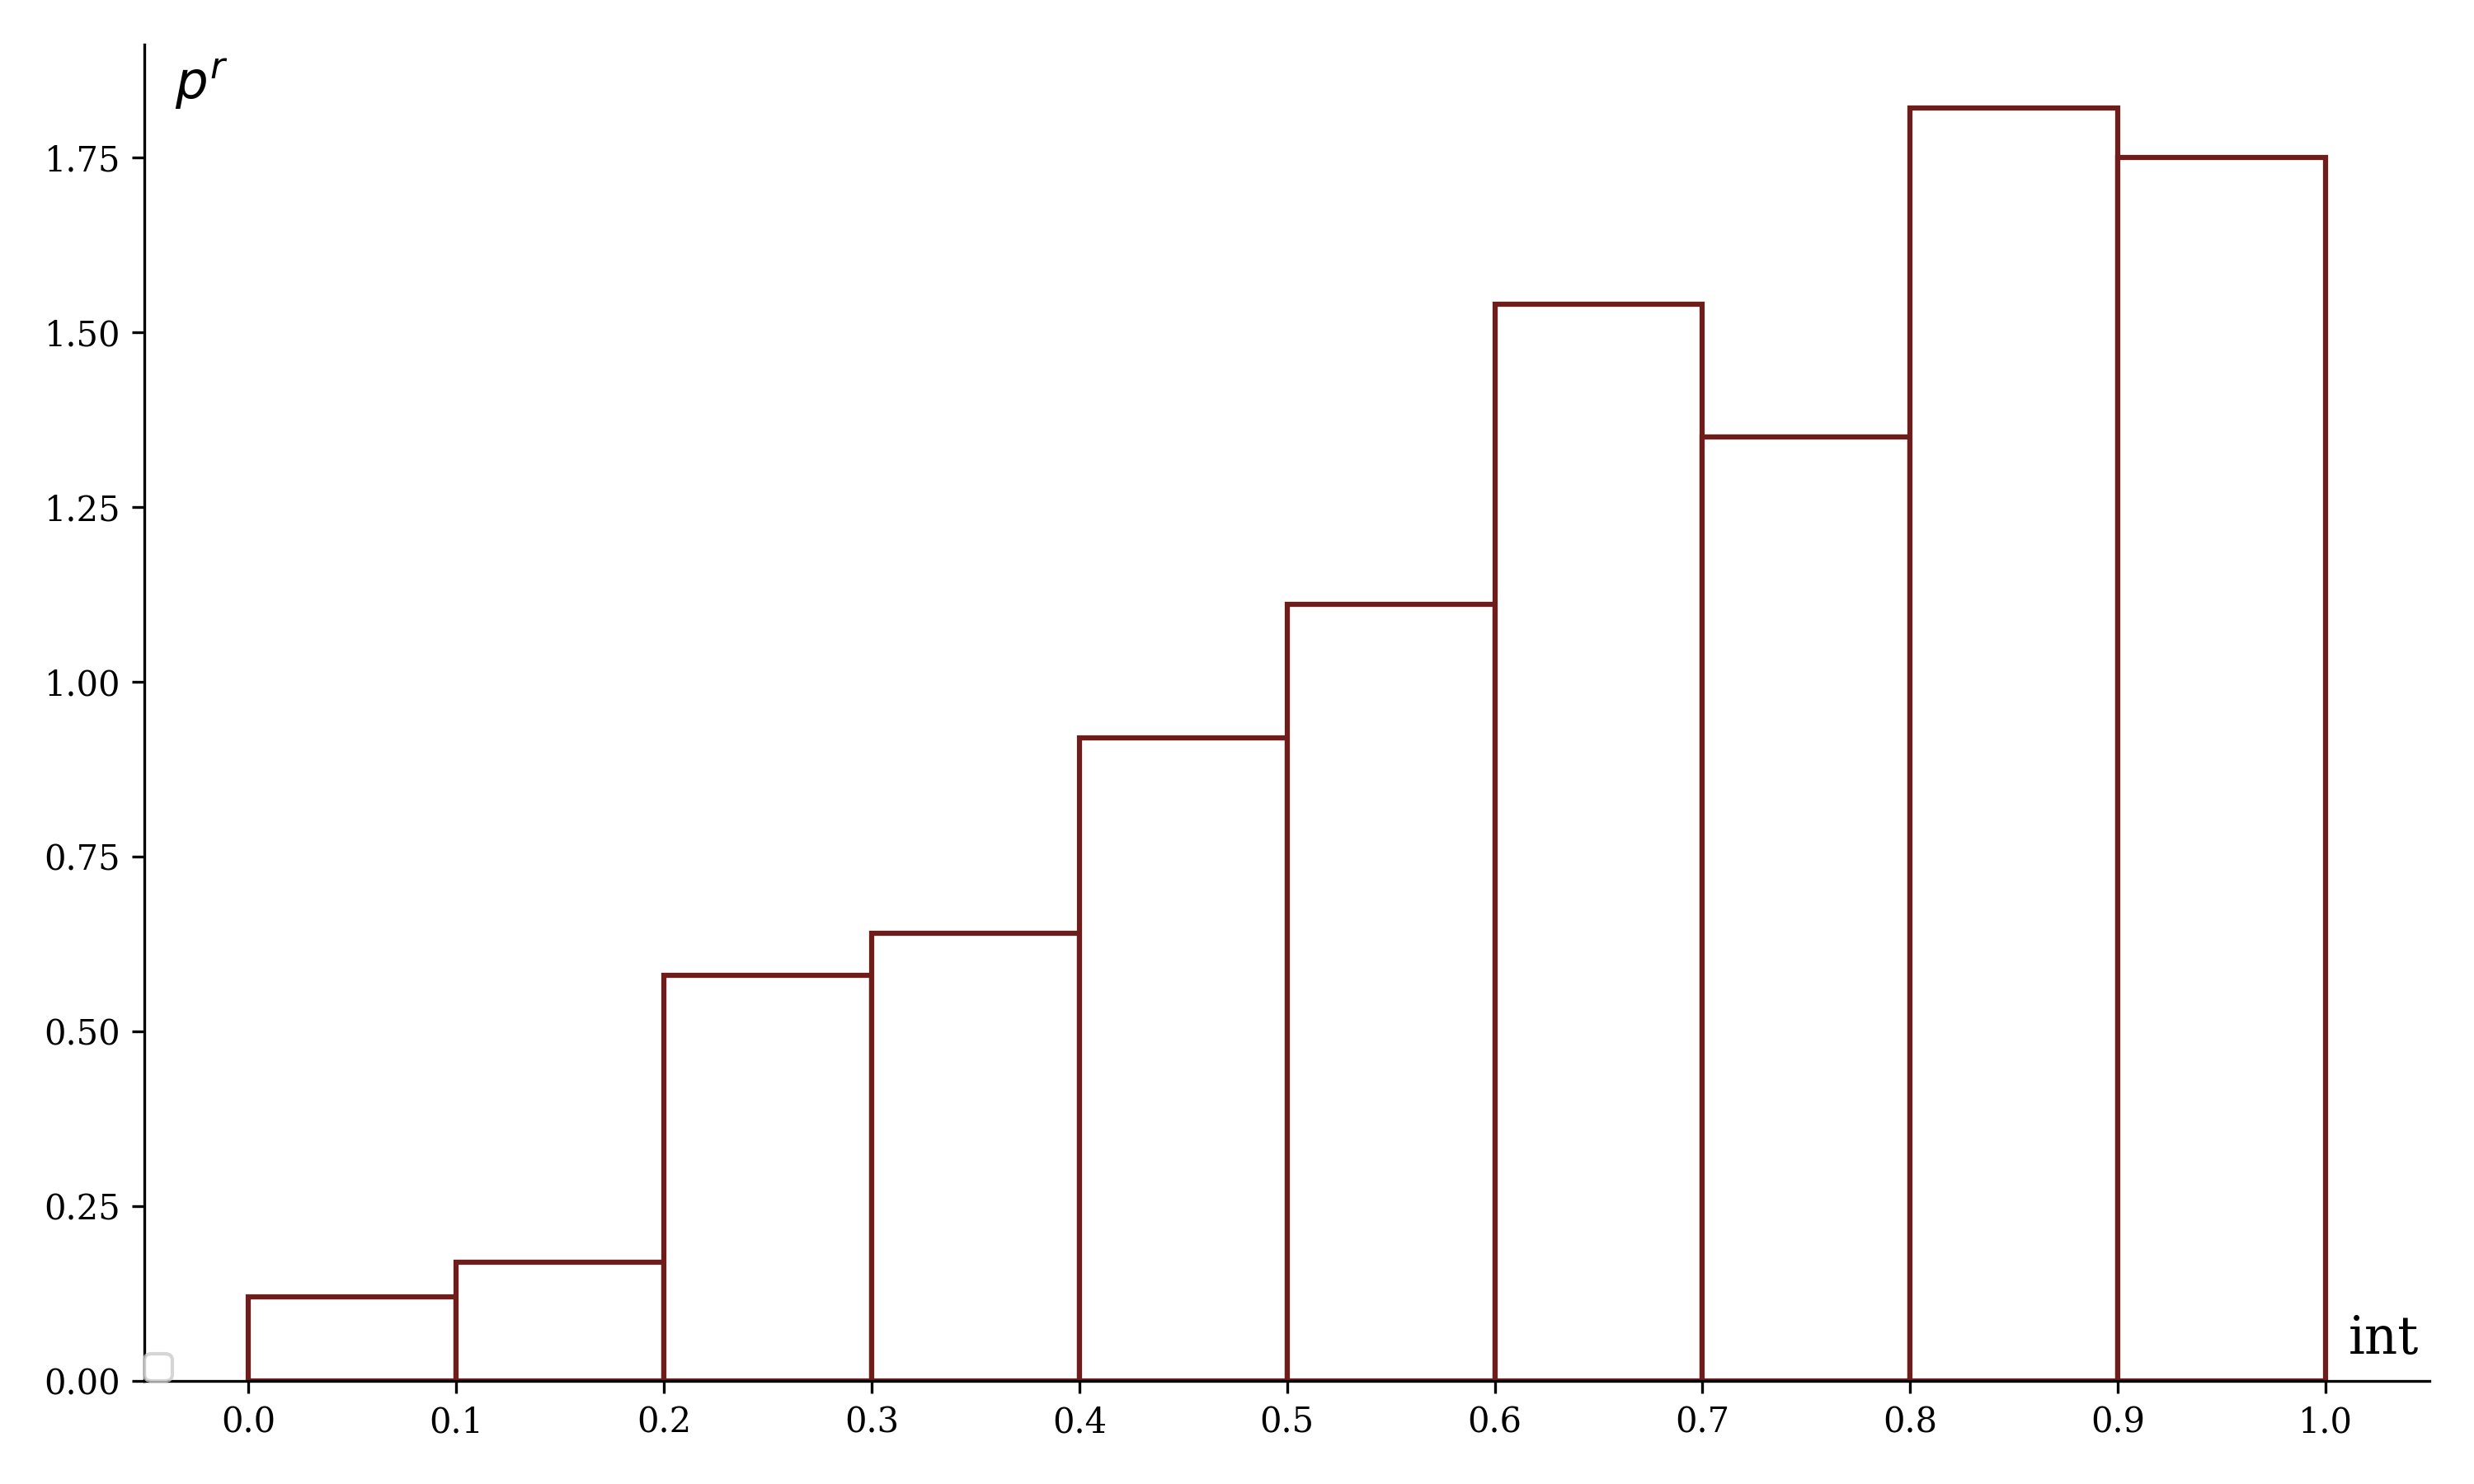
\includegraphics[width=\textwidth, height=\textheight, keepaspectratio]{sample8_hist}
\end{minipage}

\begin{minipage}[t]{0.25\textwidth}
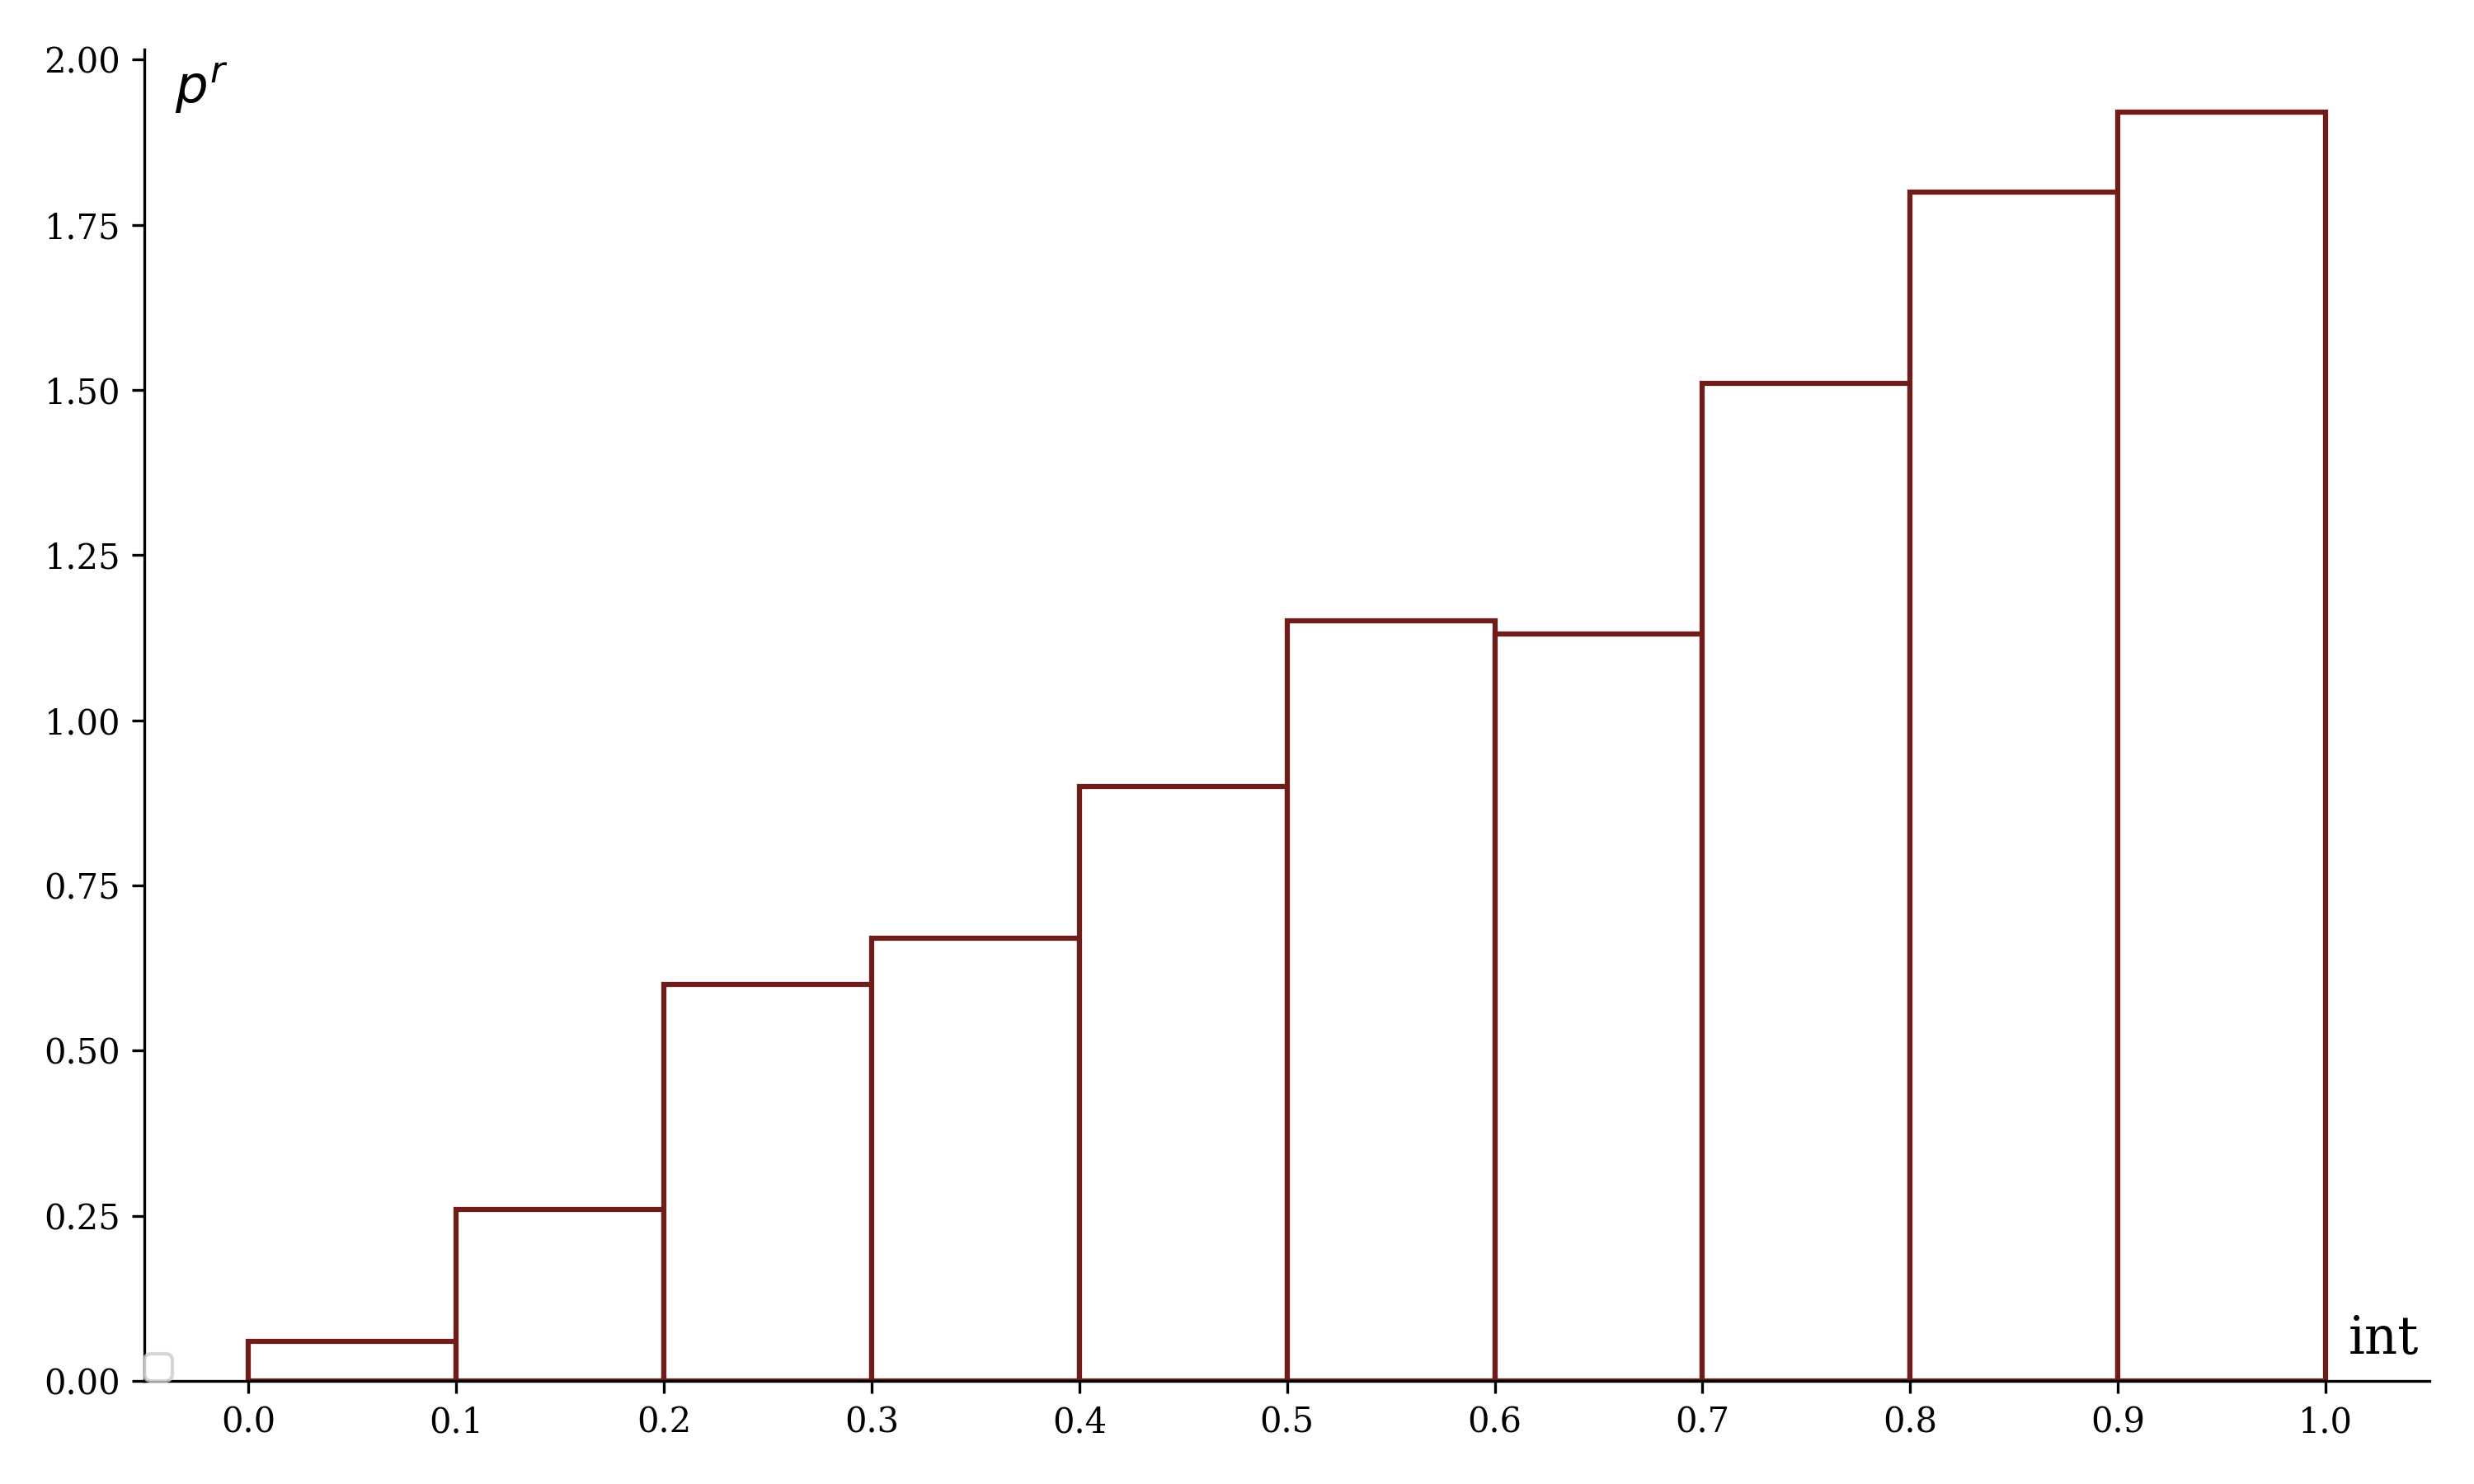
\includegraphics[width=\textwidth, height=\textheight, keepaspectratio]{sample9_hist}
\end{minipage}%
\begin{minipage}[t]{0.25\textwidth}
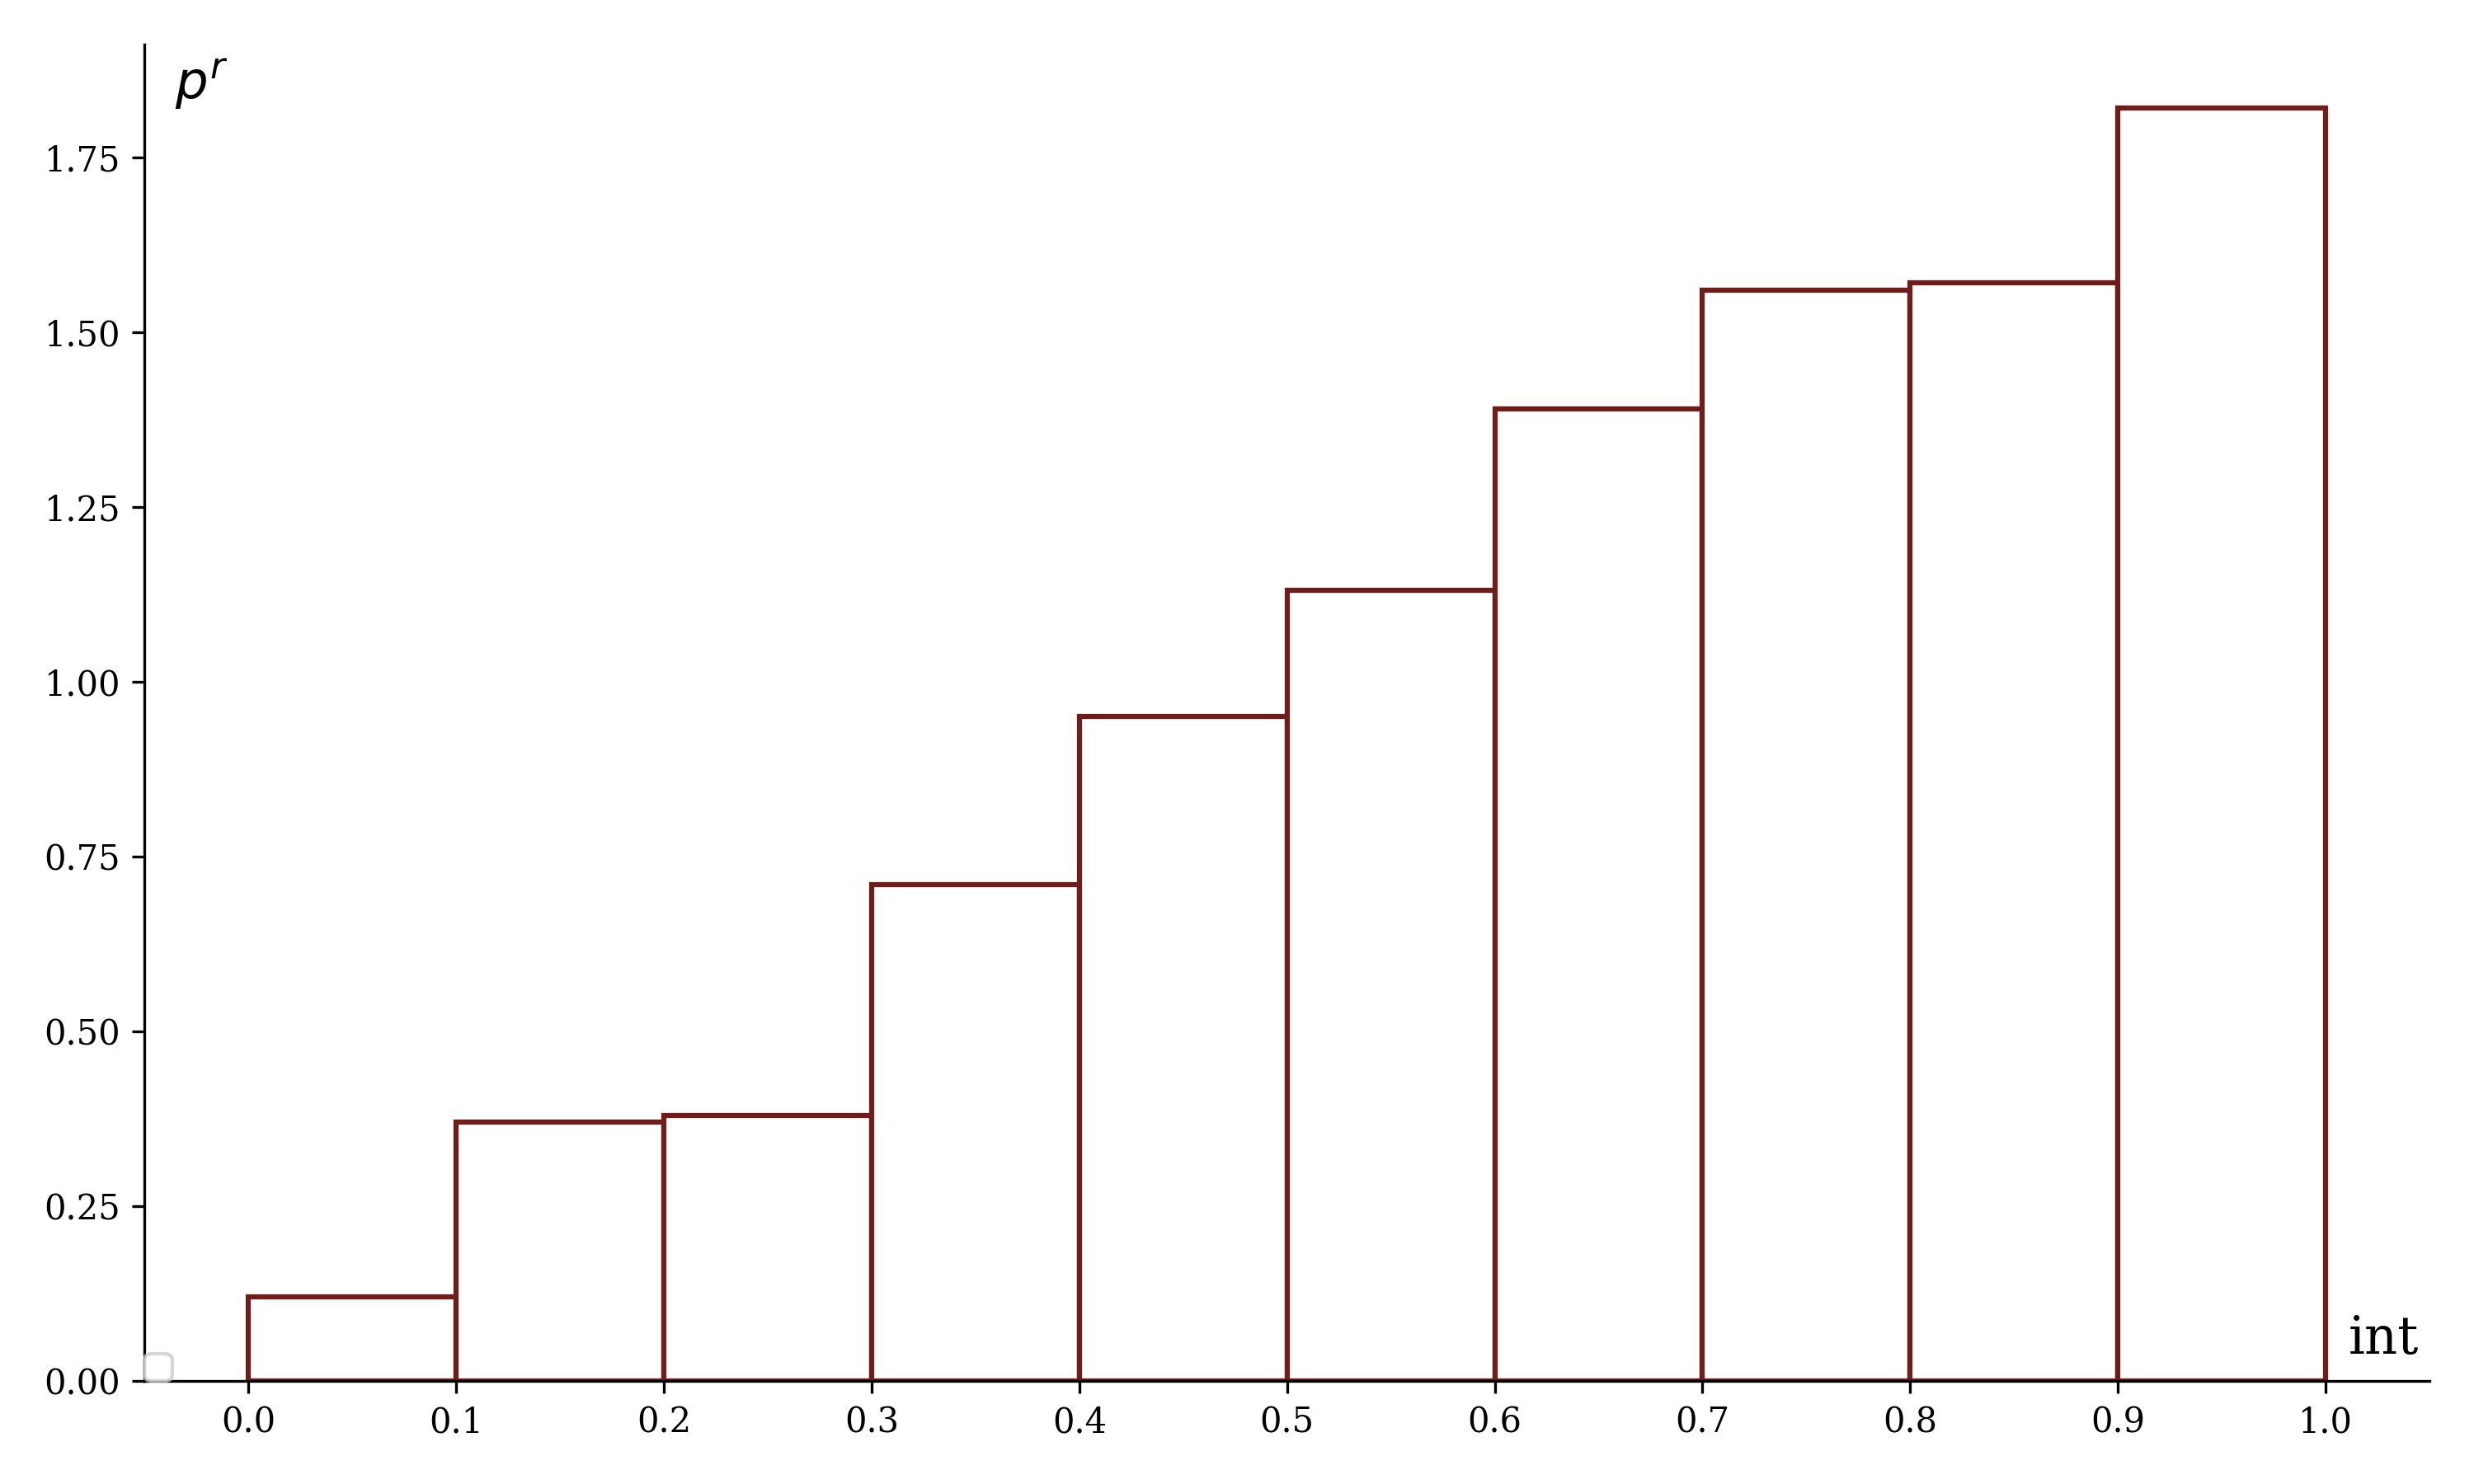
\includegraphics[width=\textwidth, height=\textheight, keepaspectratio]{sample10_hist}
\end{minipage}%
\begin{minipage}[t]{0.25\textwidth}
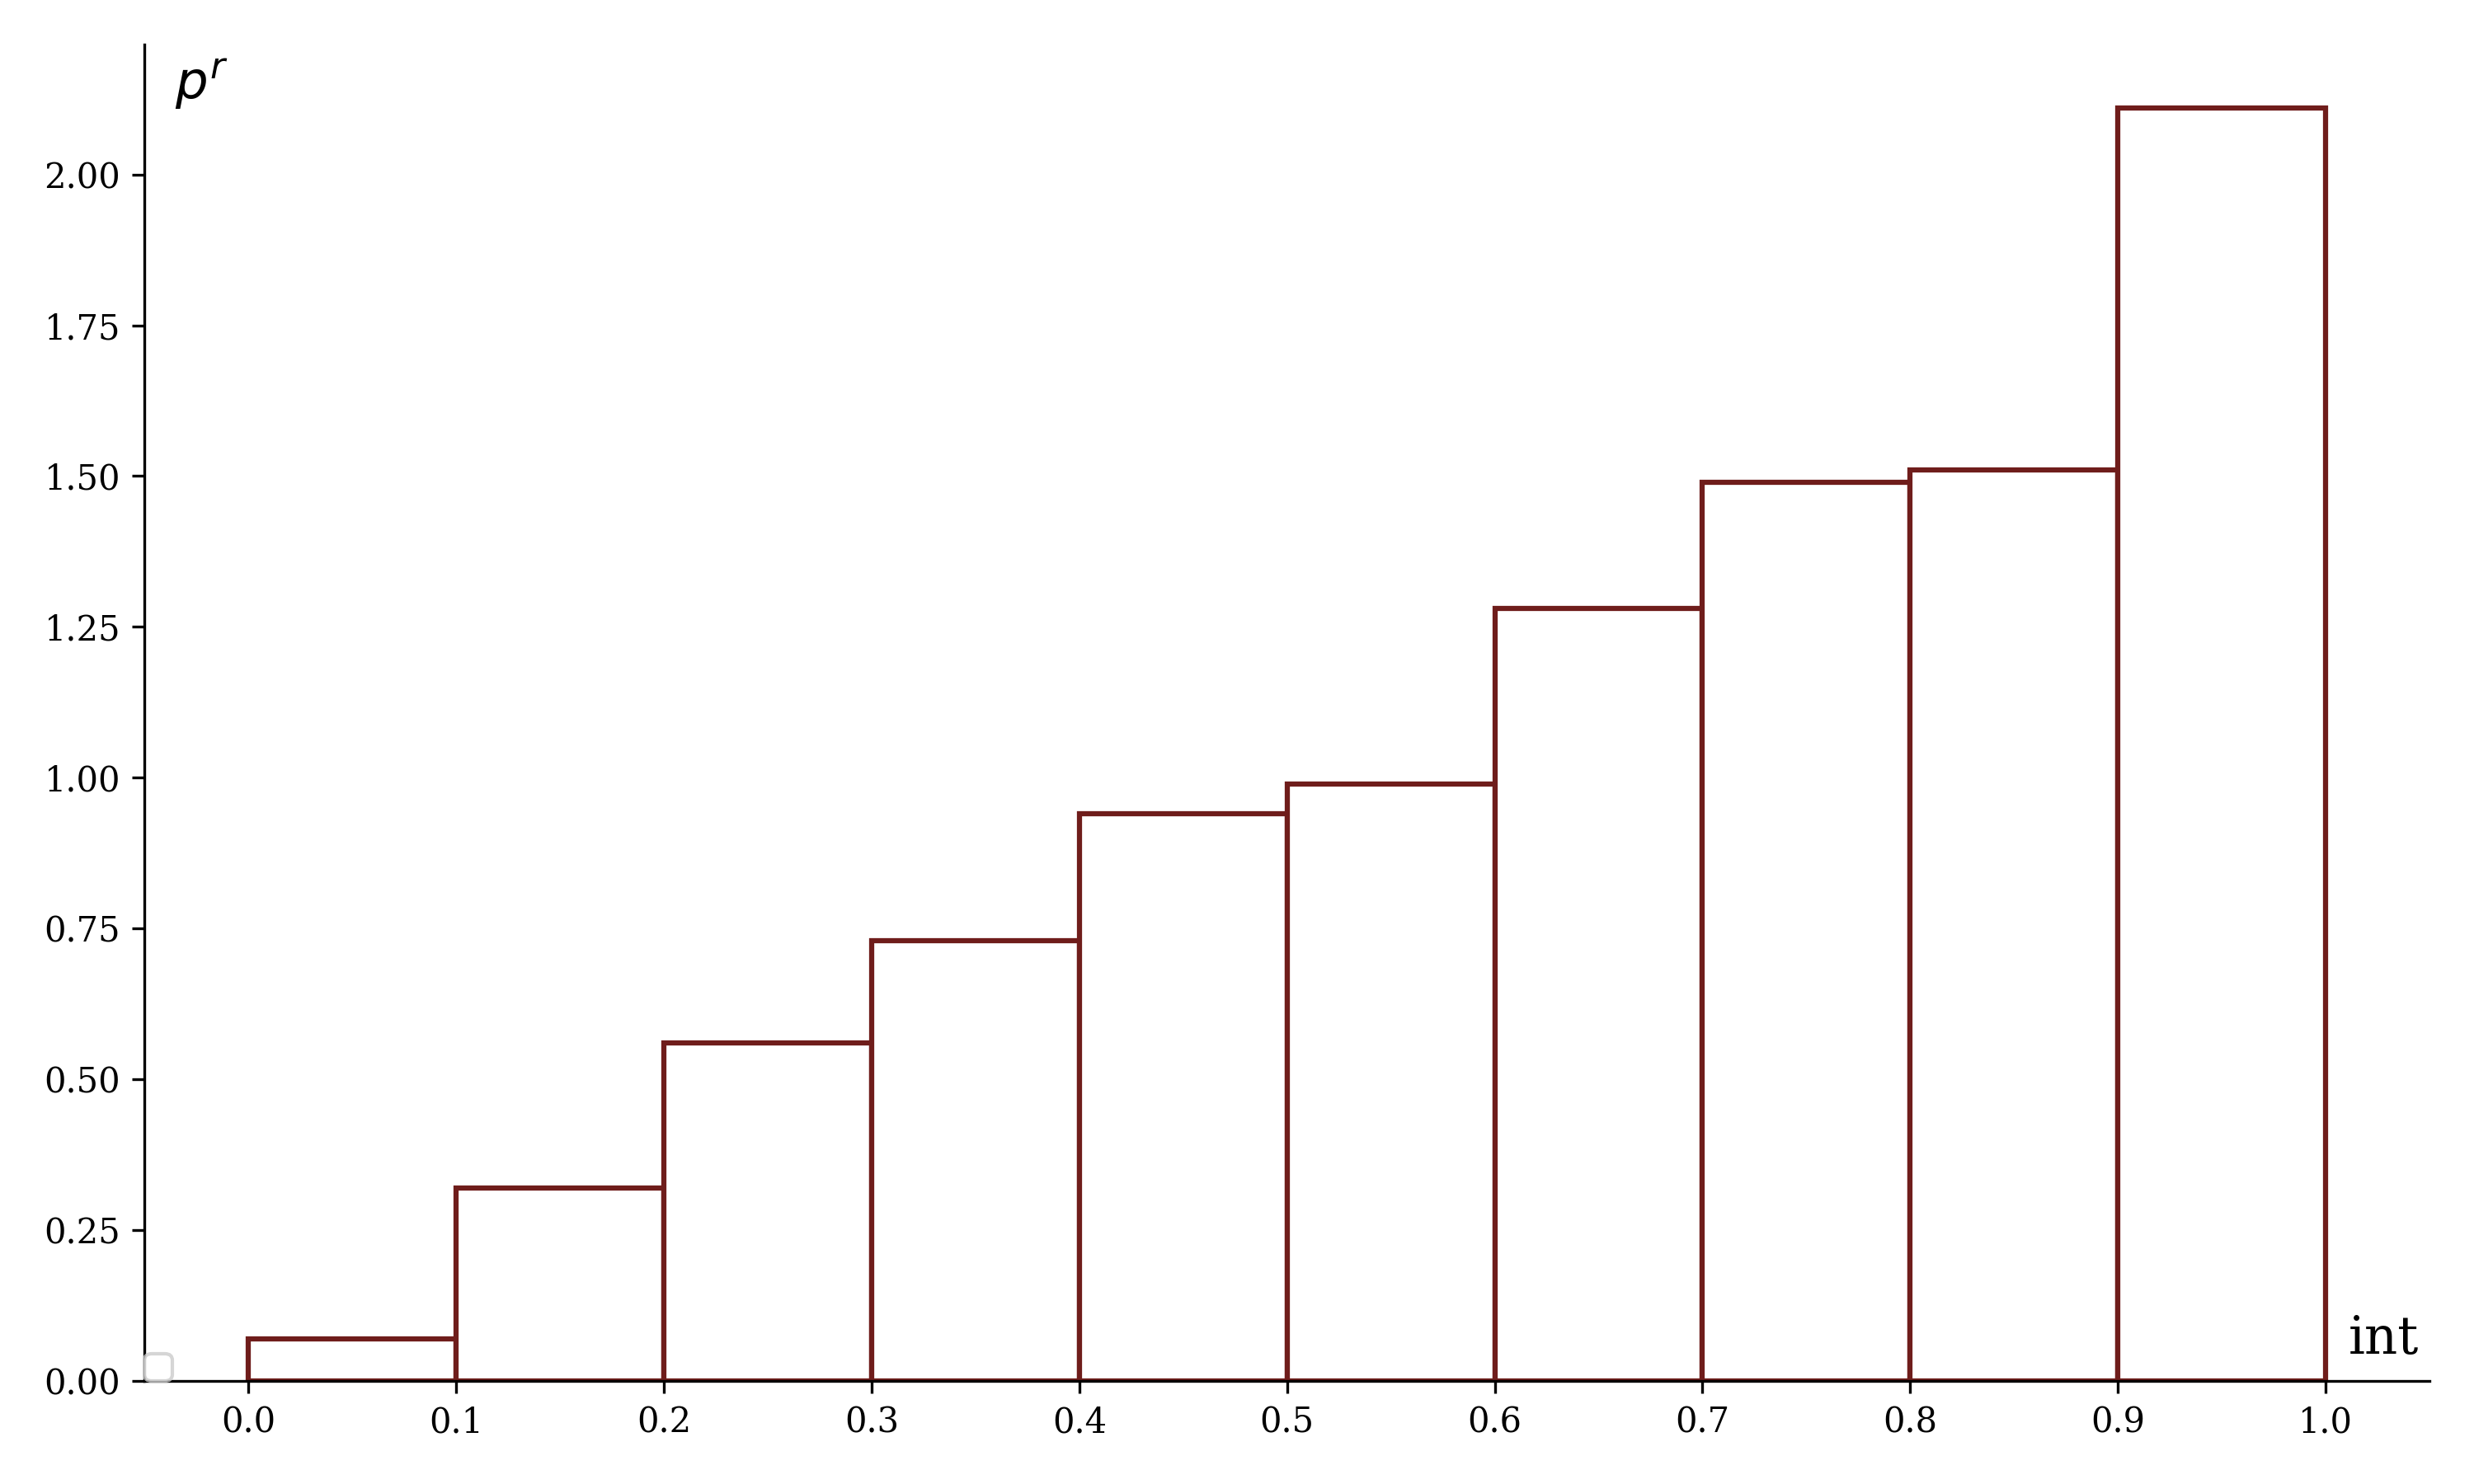
\includegraphics[width=\textwidth, height=\textheight, keepaspectratio]{sample11_hist}
\end{minipage}%
\begin{minipage}[t]{0.25\textwidth}
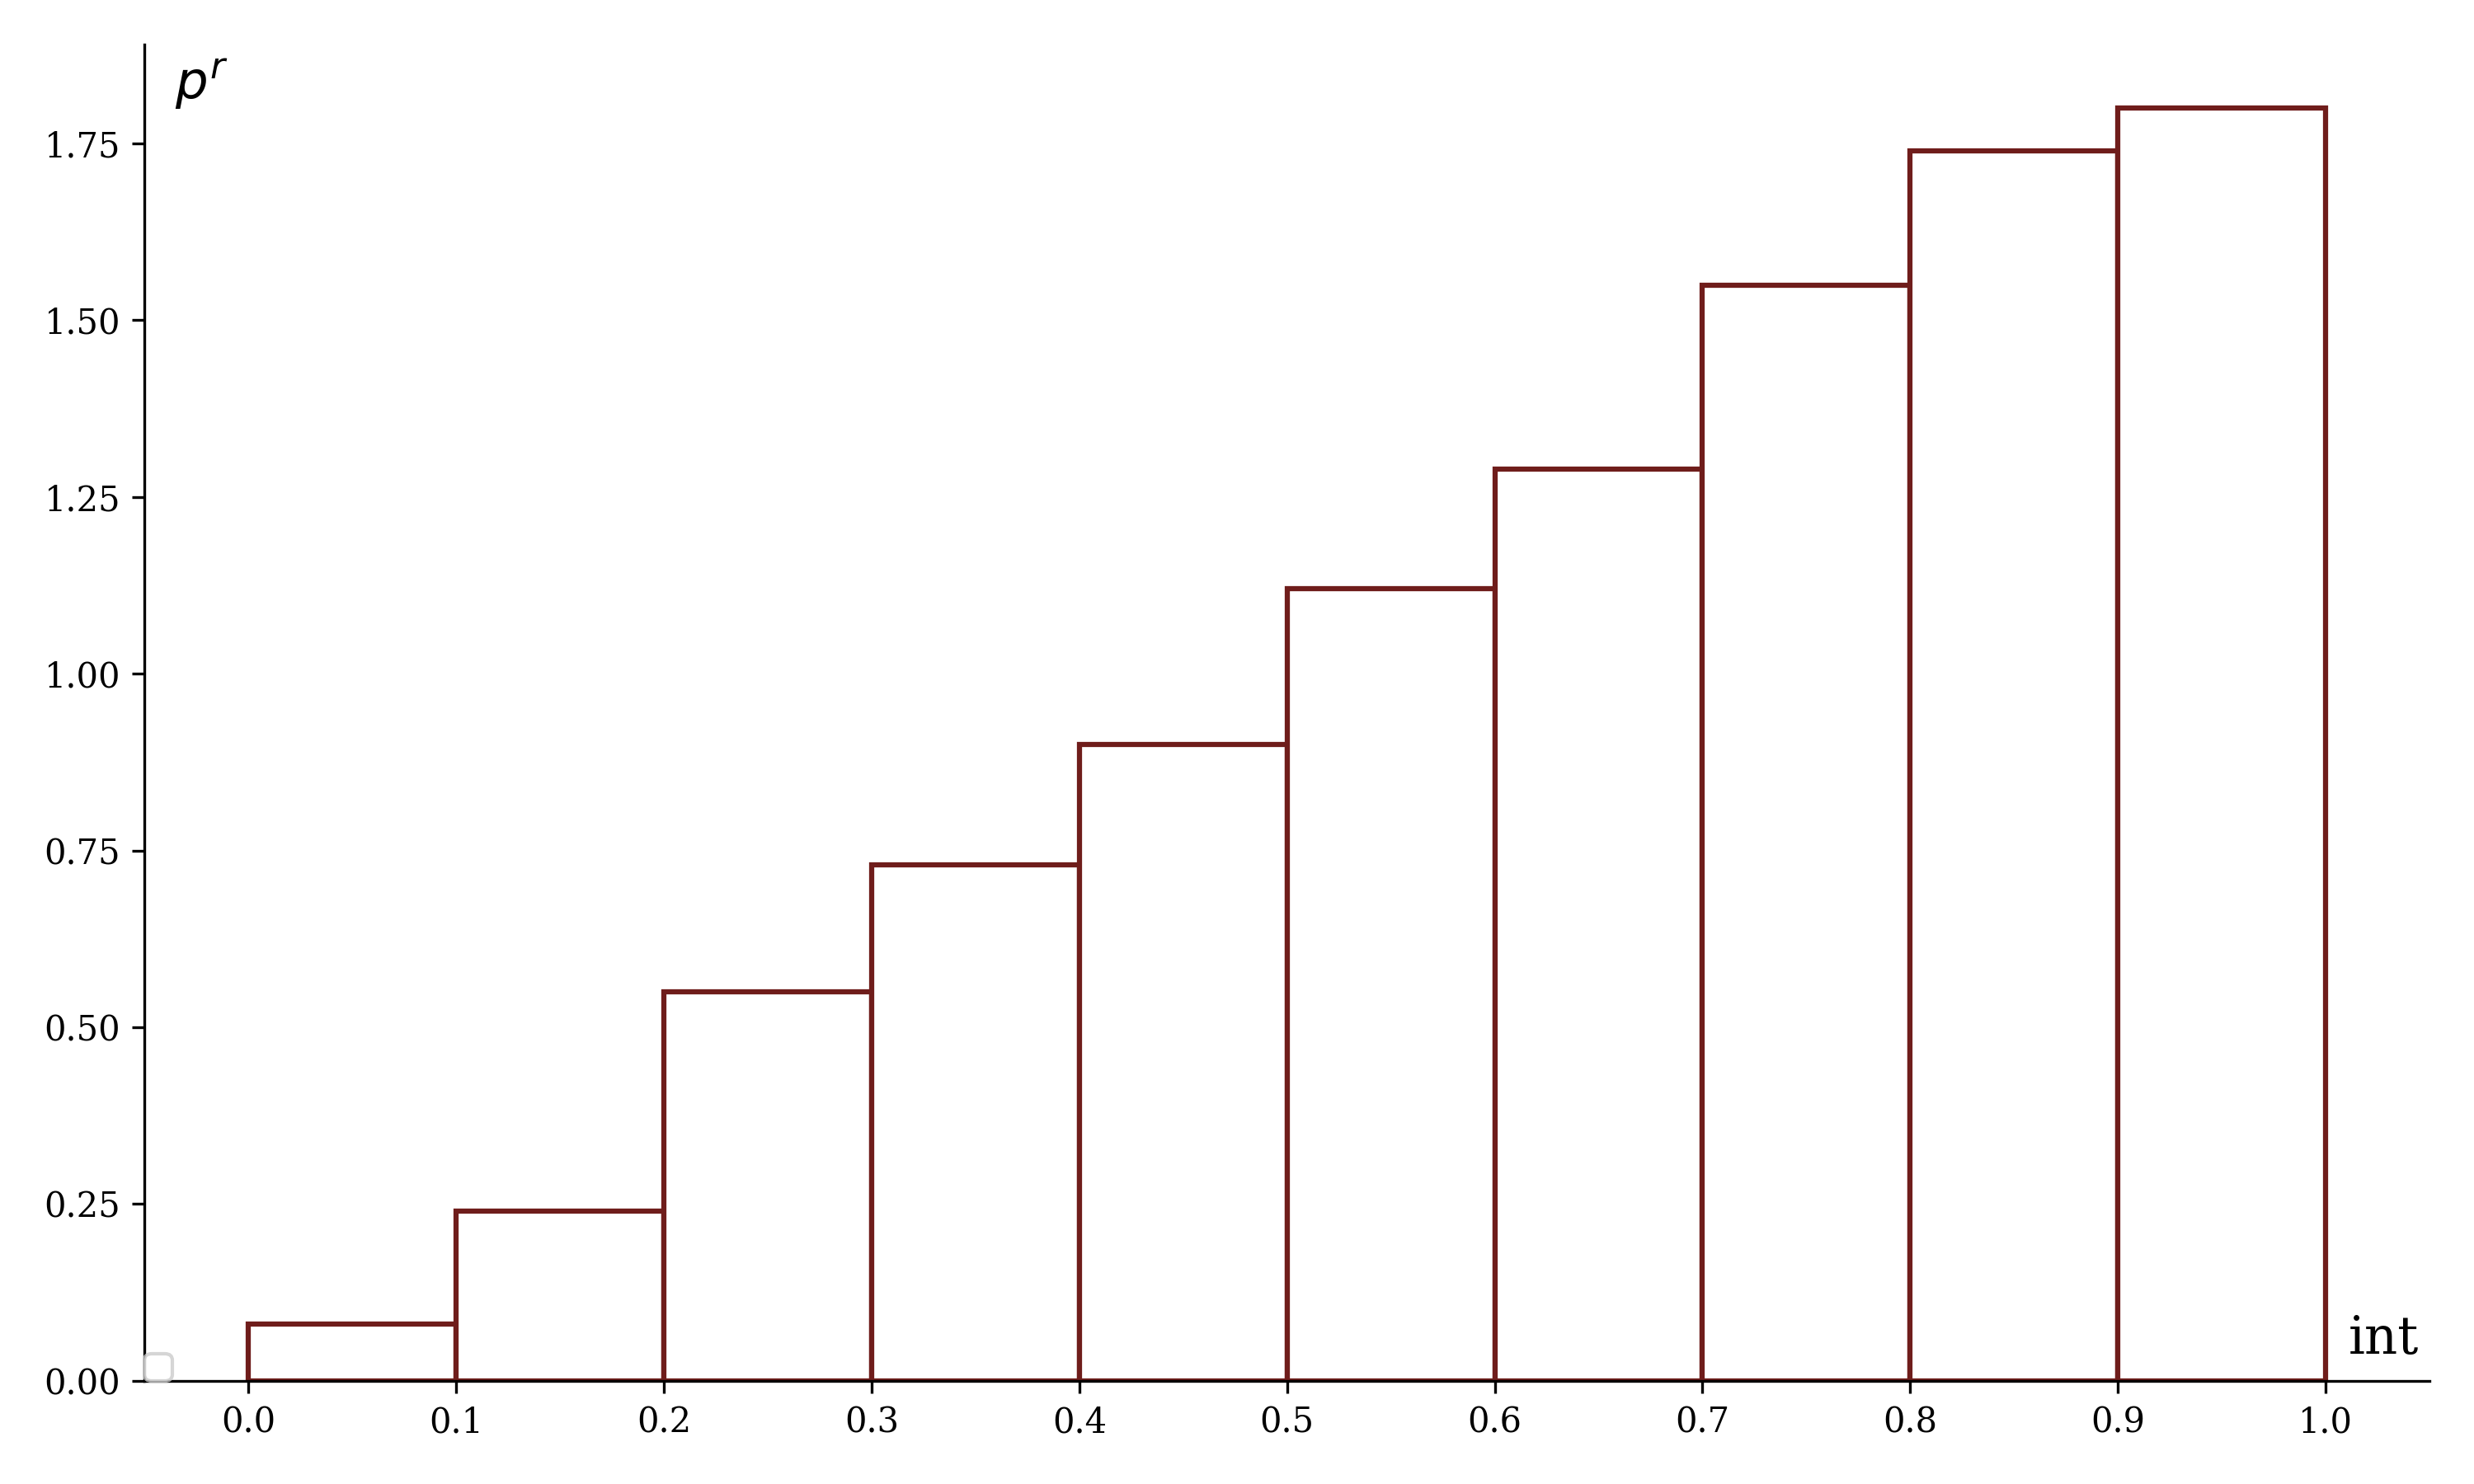
\includegraphics[width=\textwidth, height=\textheight, keepaspectratio]{sample12_hist}
\end{minipage}

\begin{minipage}[t]{0.25\textwidth}
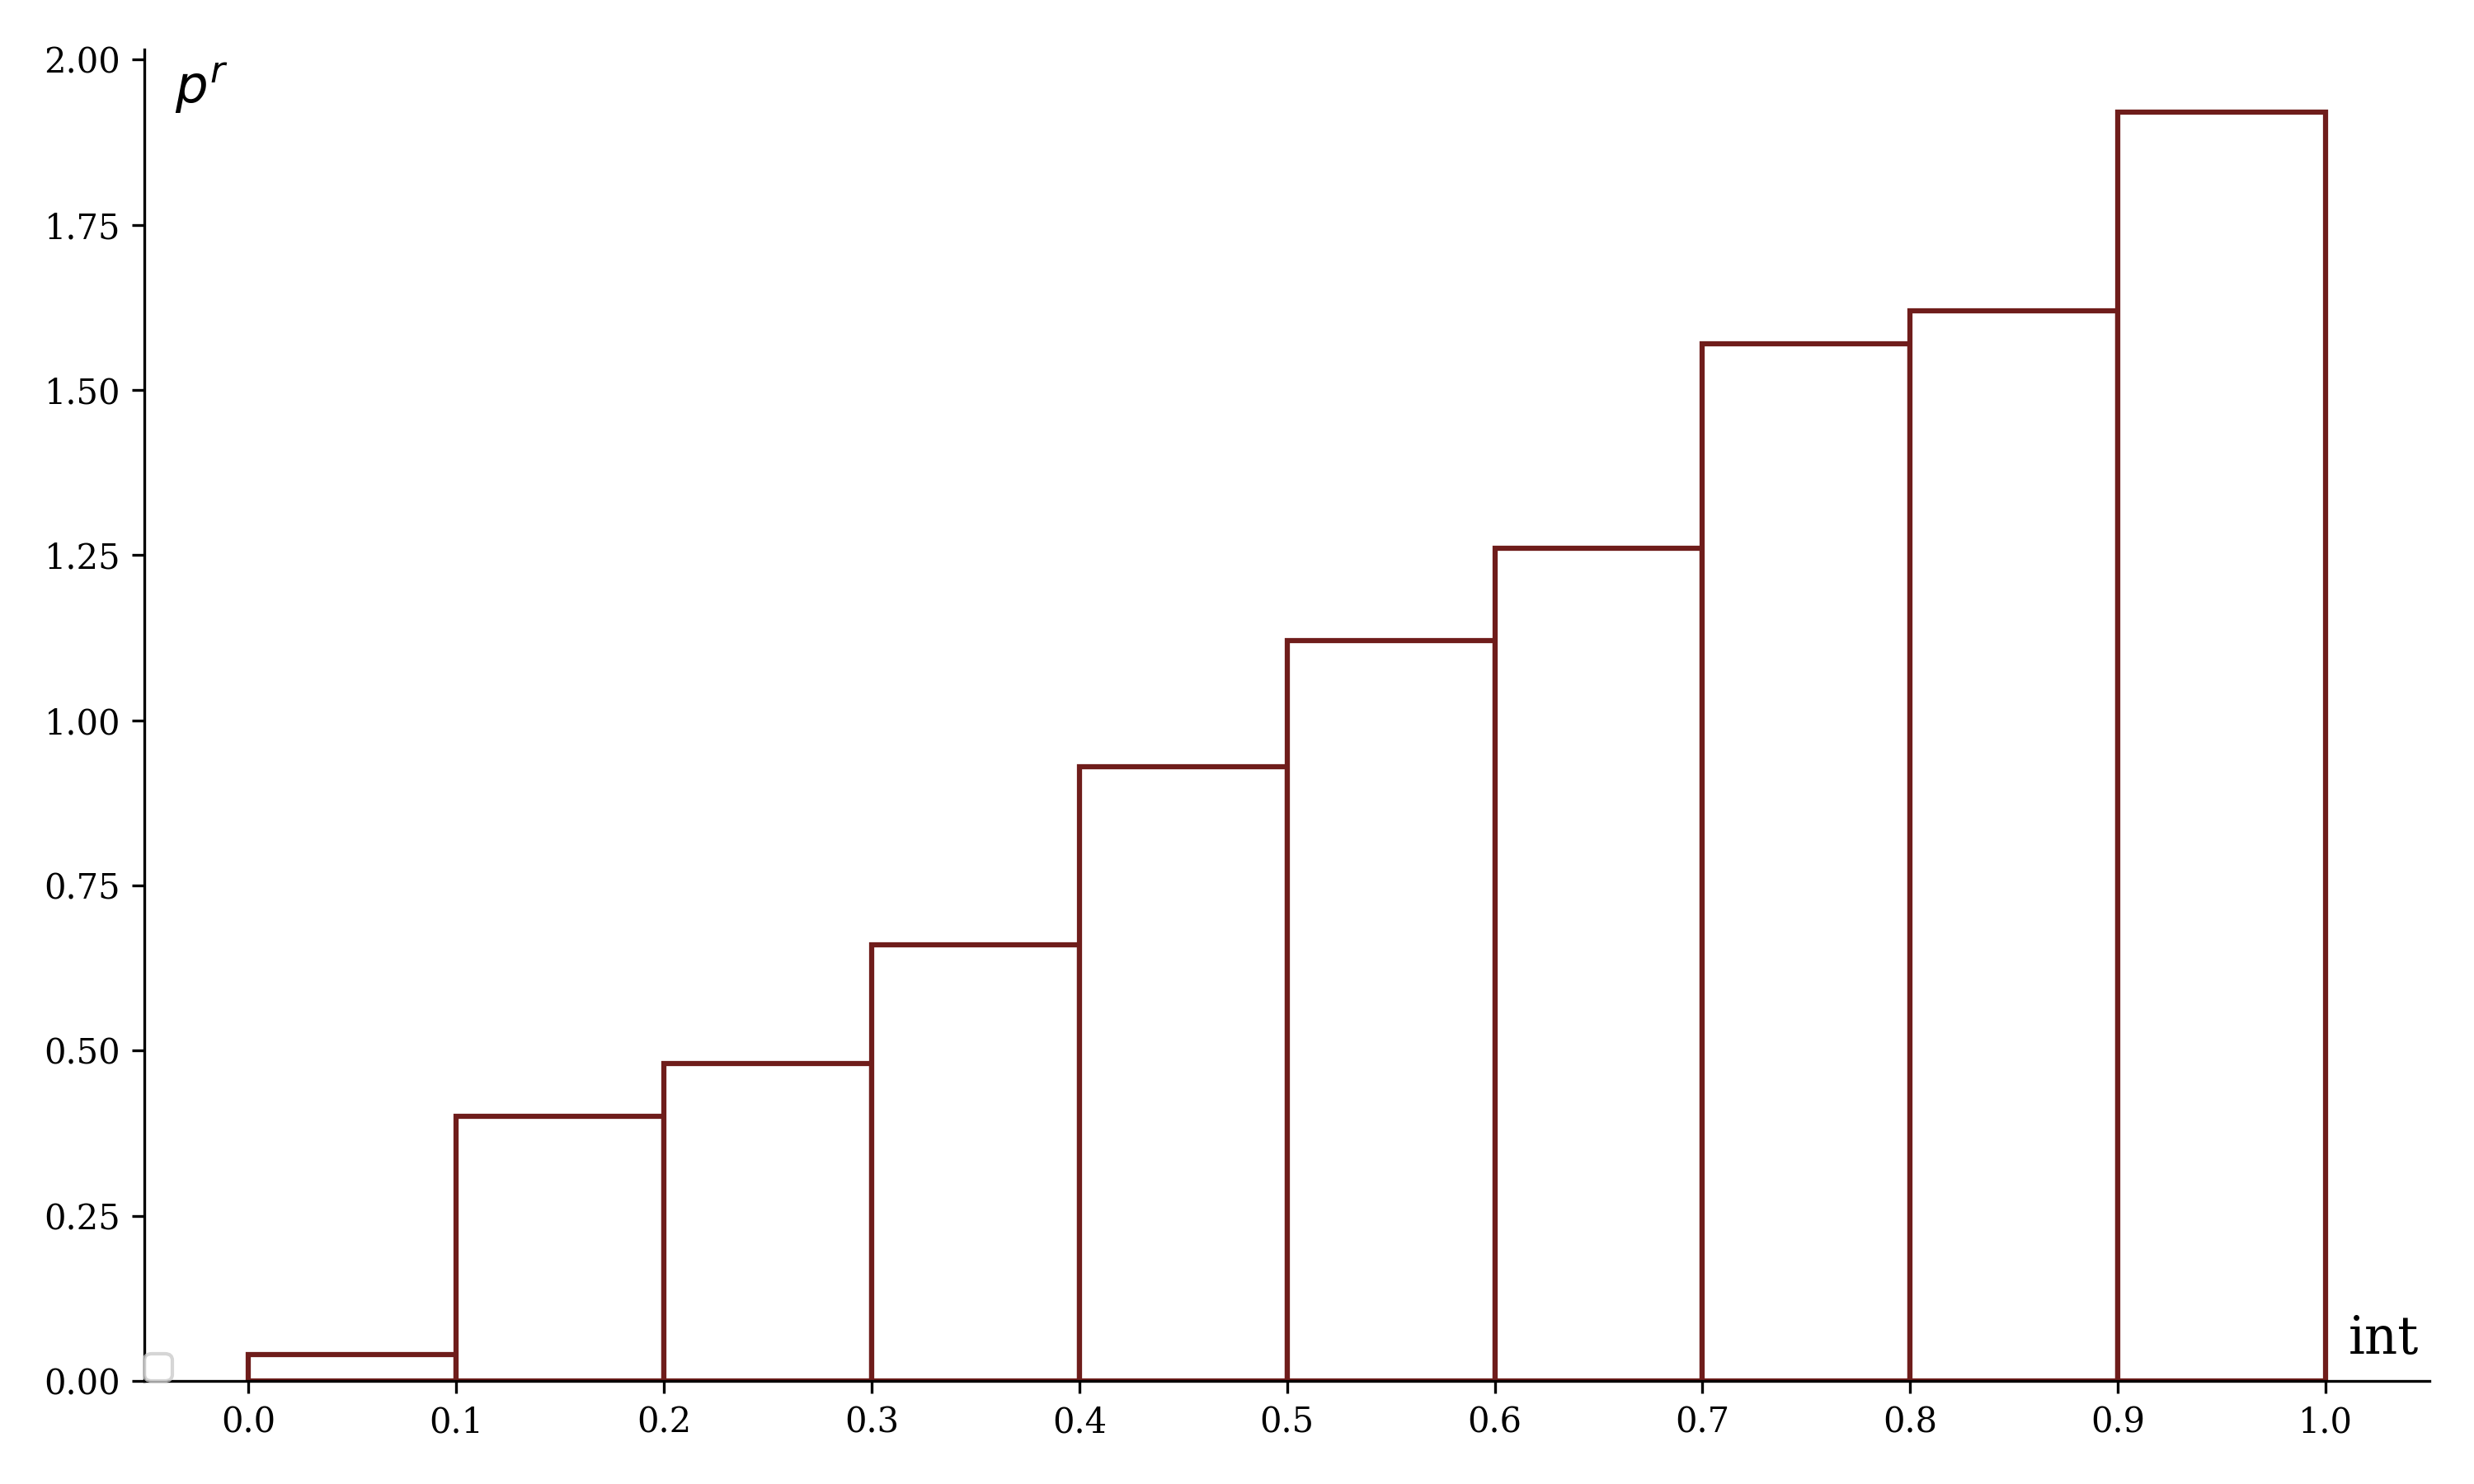
\includegraphics[width=\textwidth, height=\textheight, keepaspectratio]{sample13_hist}
\end{minipage}%
\begin{minipage}[t]{0.25\textwidth}
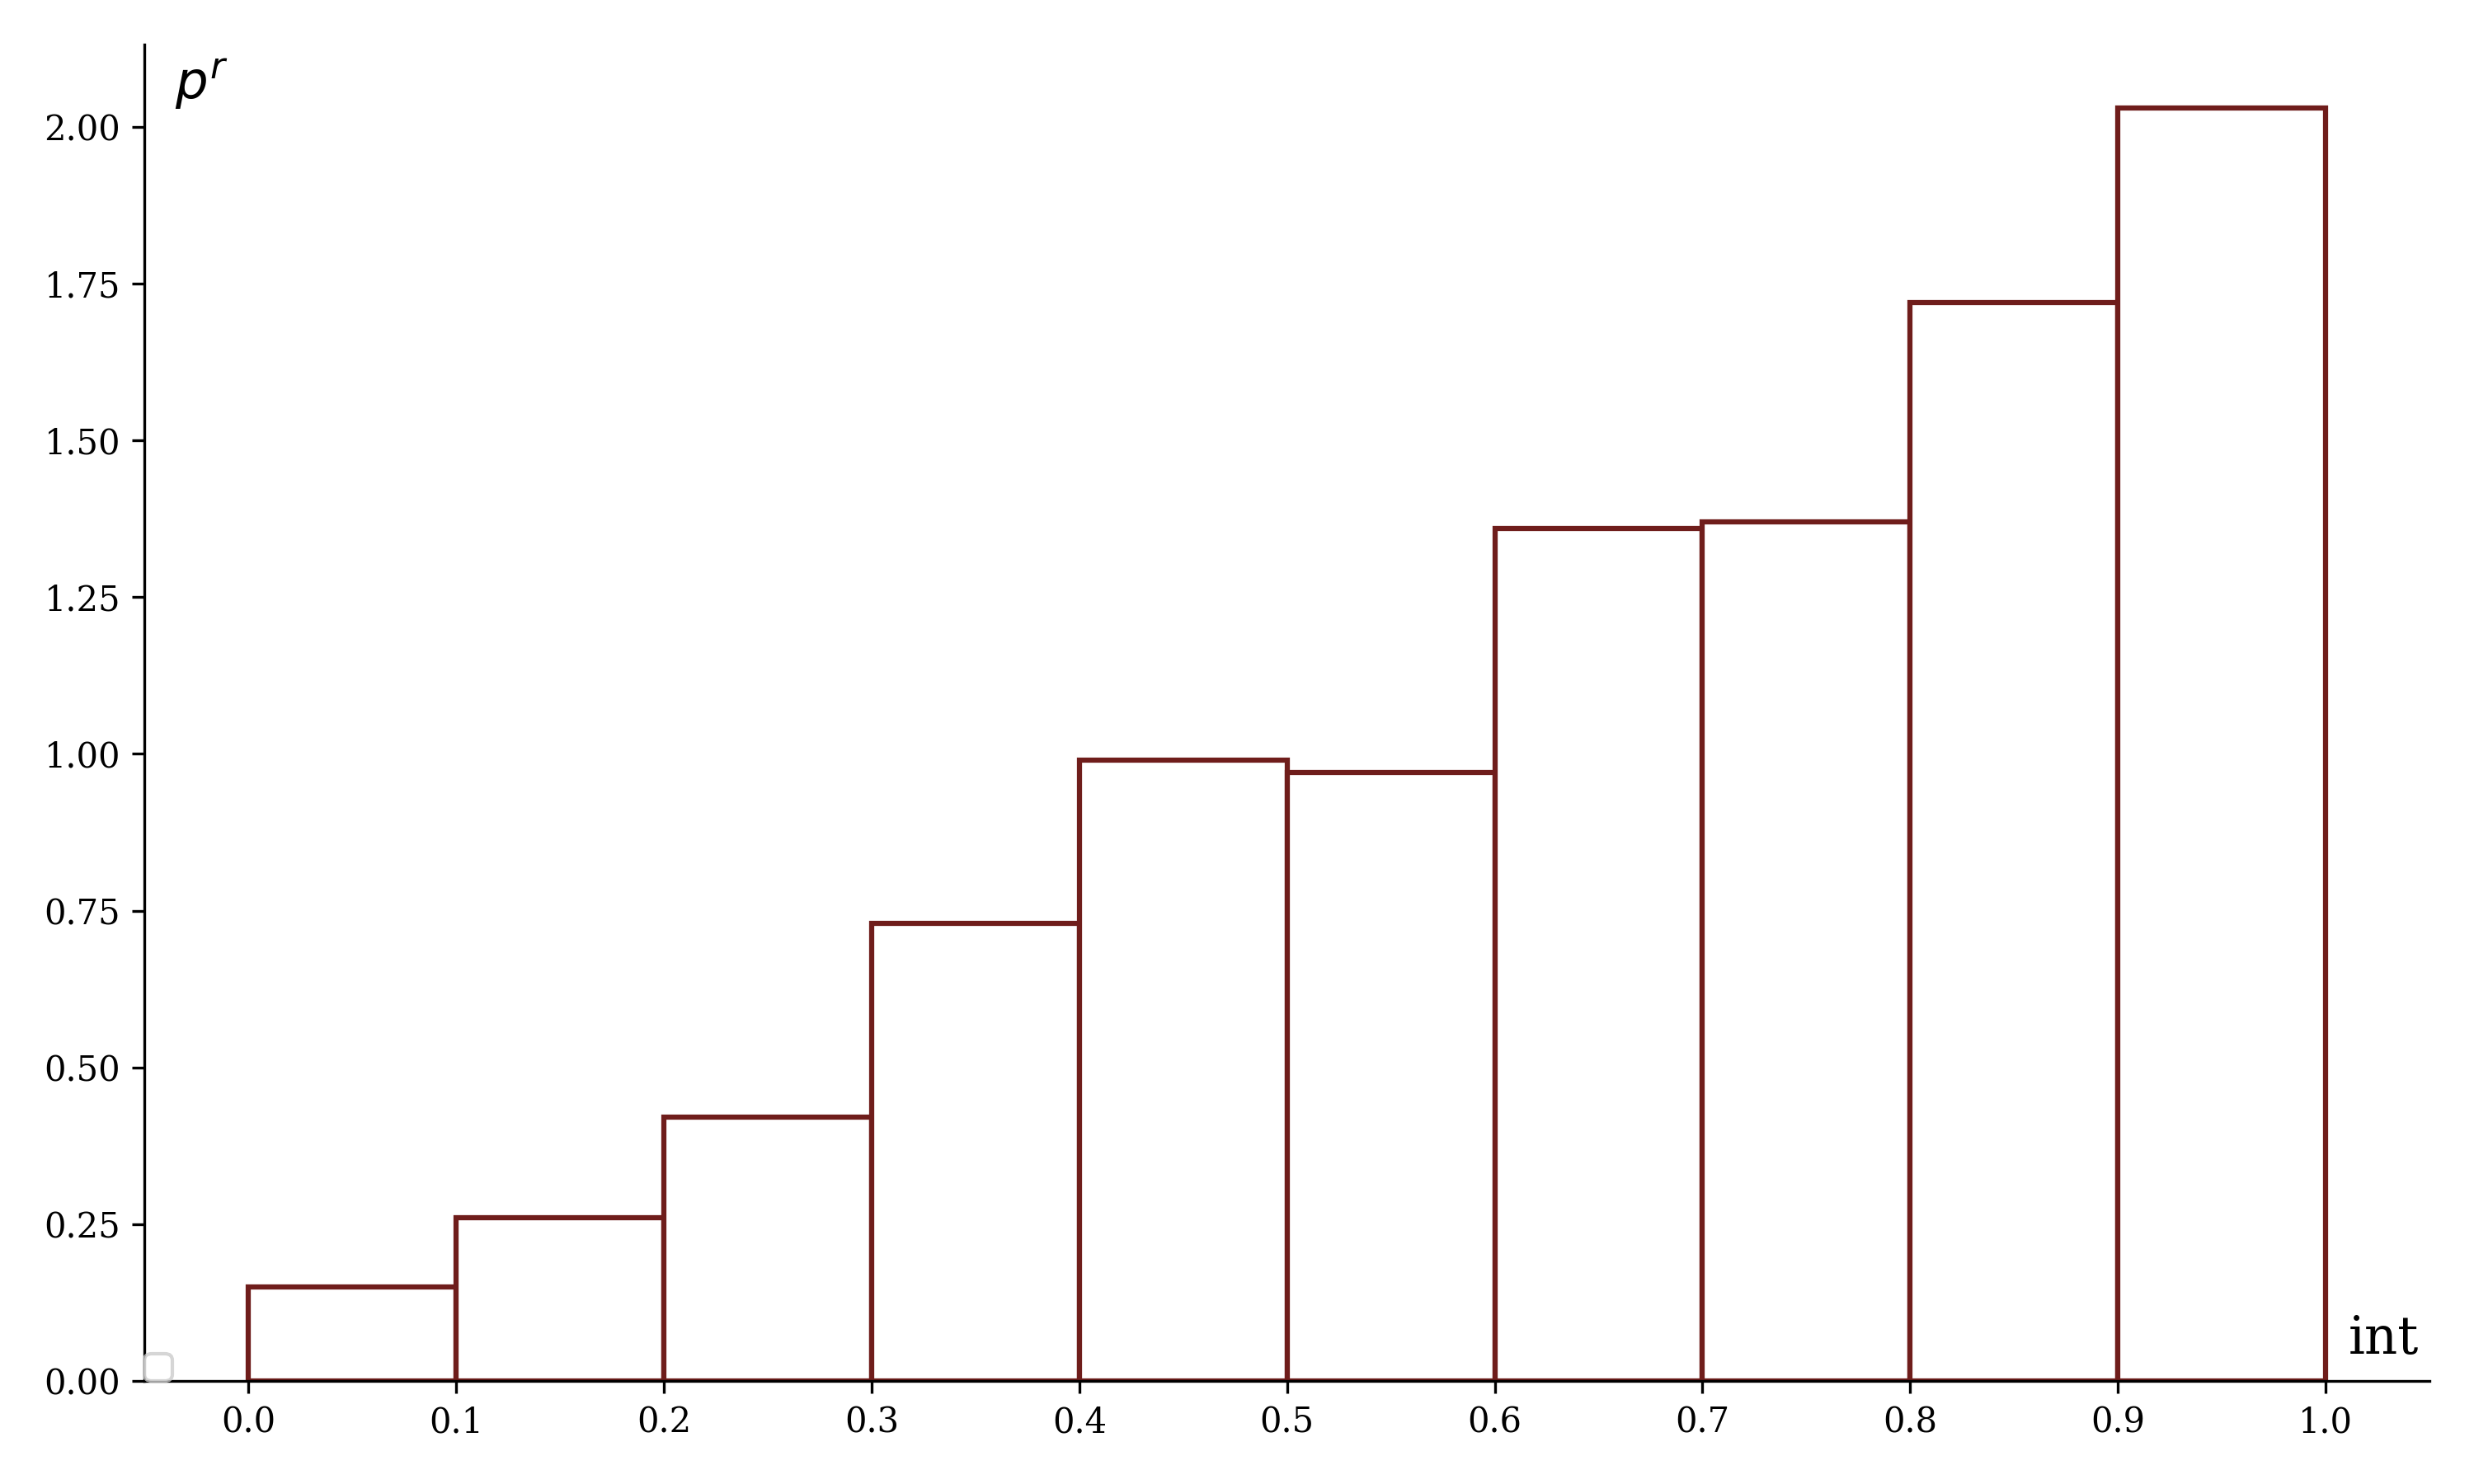
\includegraphics[width=\textwidth, height=\textheight, keepaspectratio]{sample14_hist}
\end{minipage}%
\begin{minipage}[t]{0.25\textwidth}
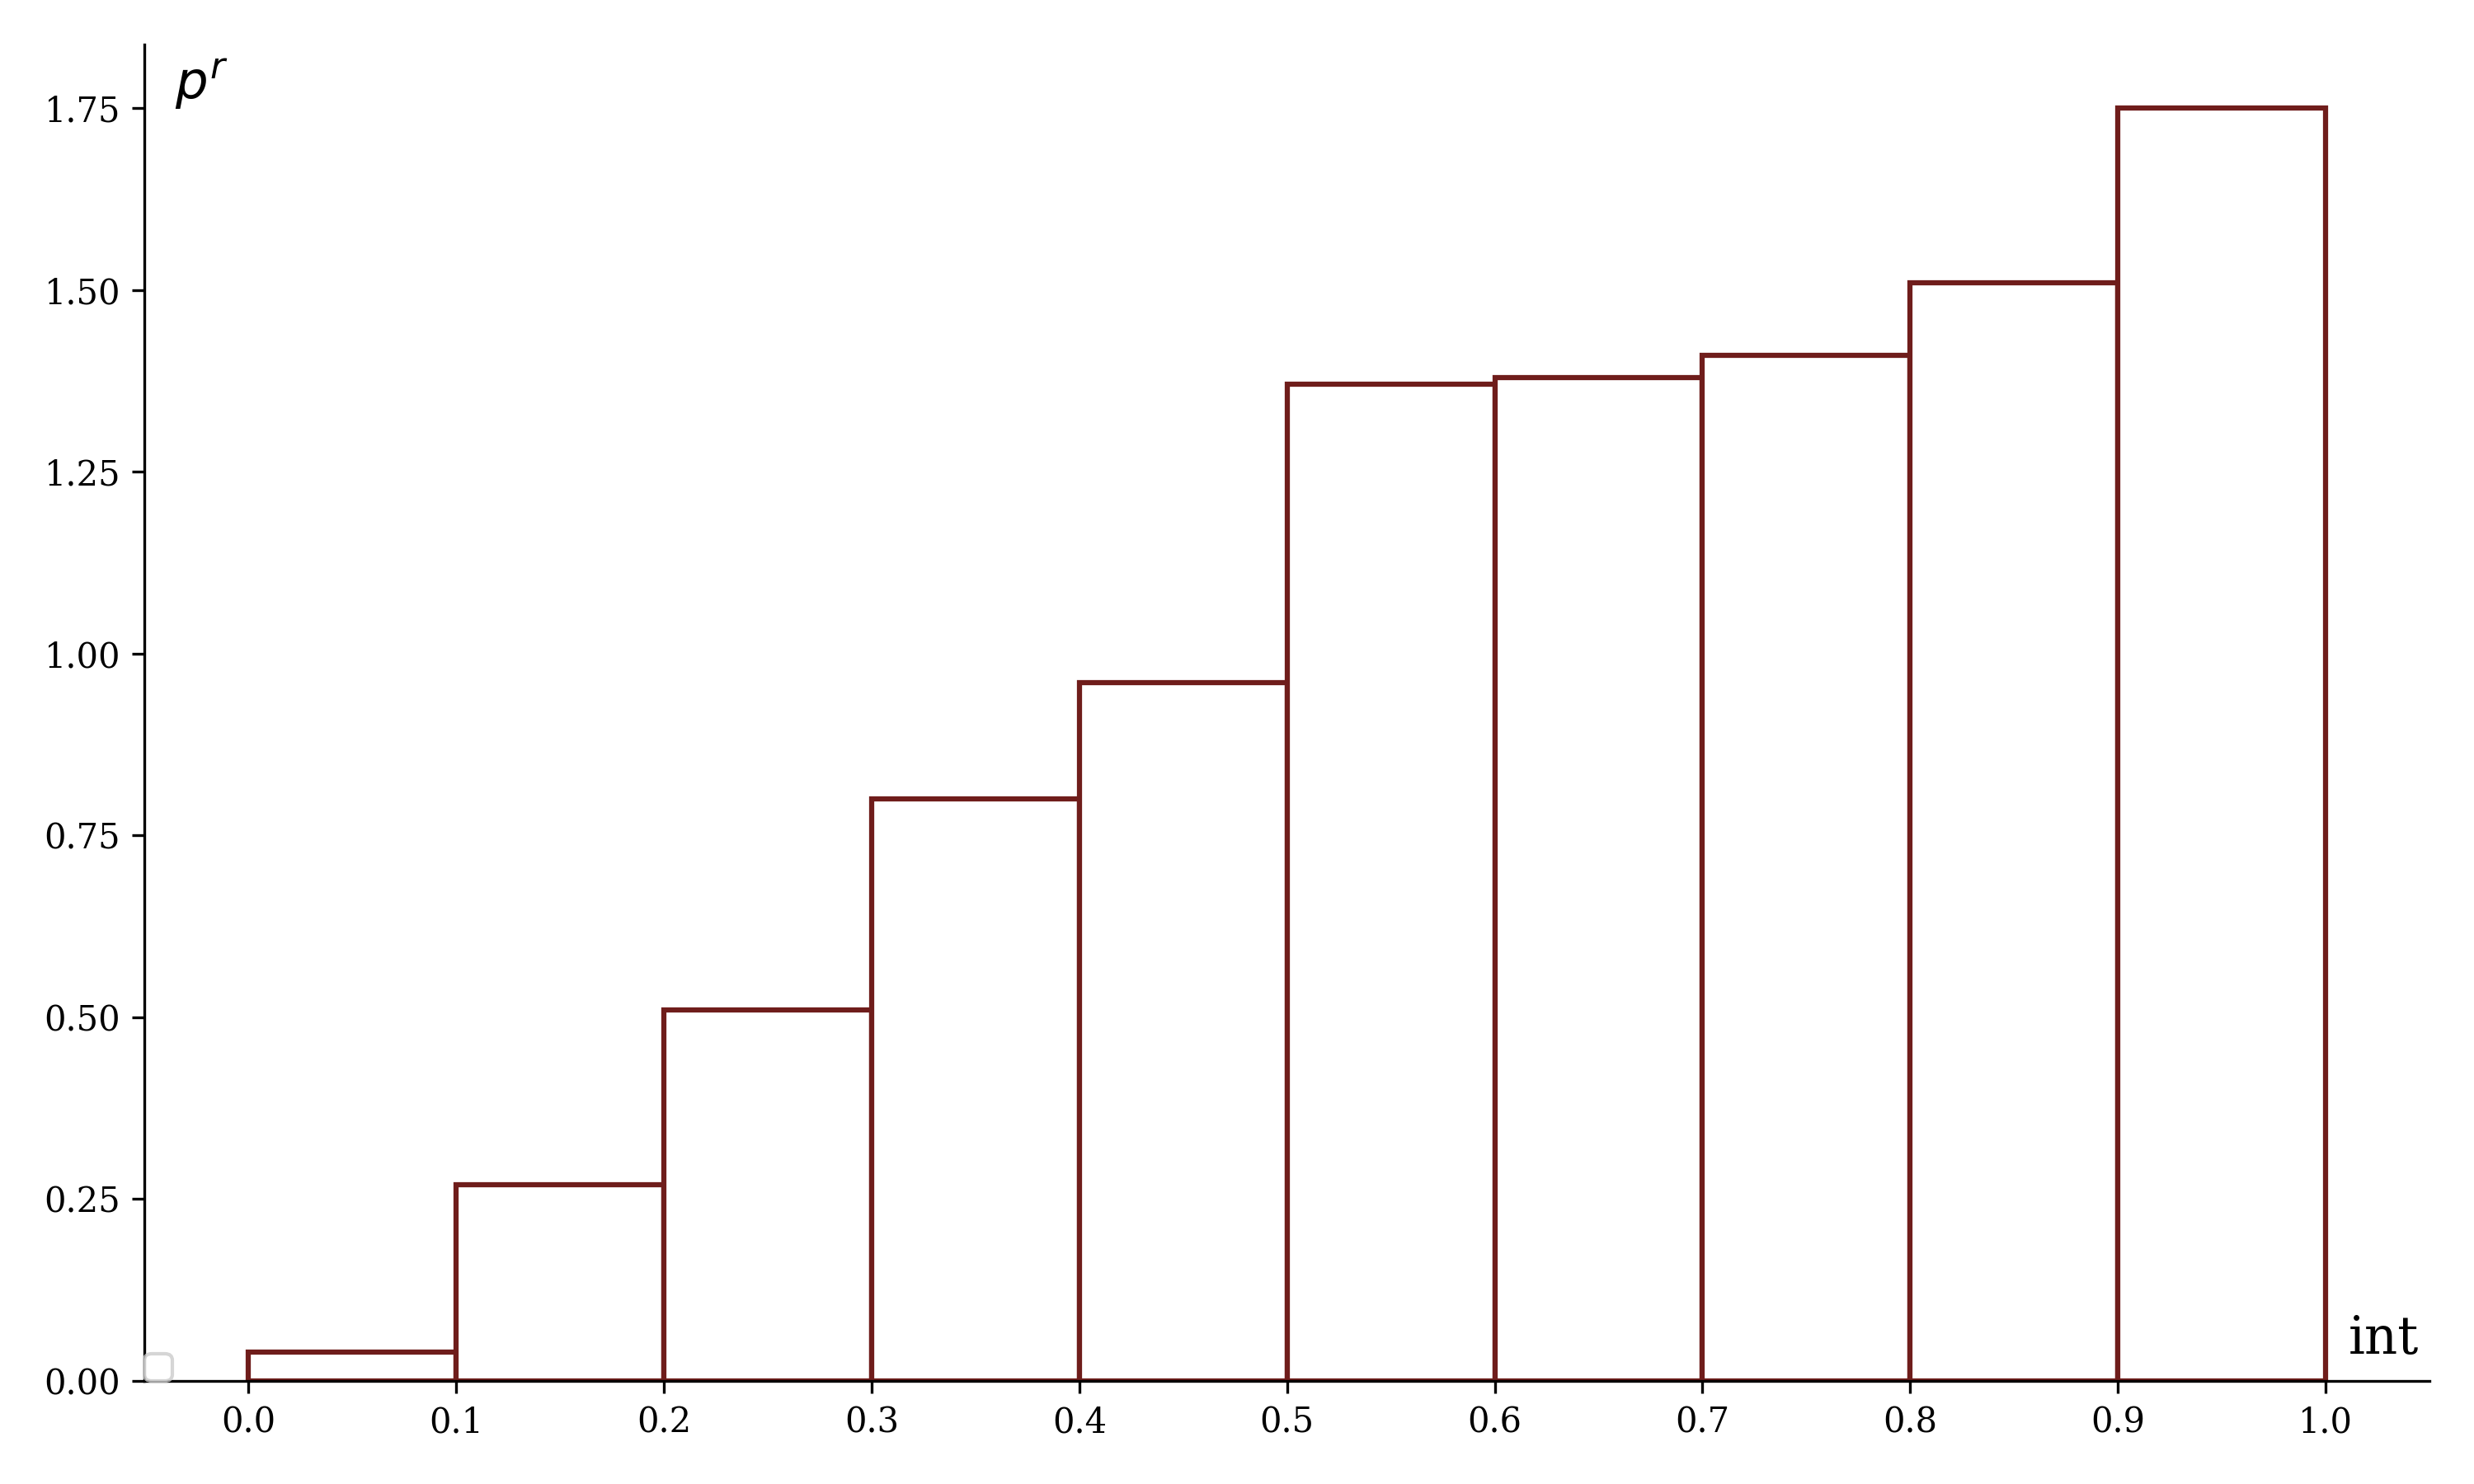
\includegraphics[width=\textwidth, height=\textheight, keepaspectratio]{sample15_hist}
\end{minipage}%
\begin{minipage}[t]{0.25\textwidth}
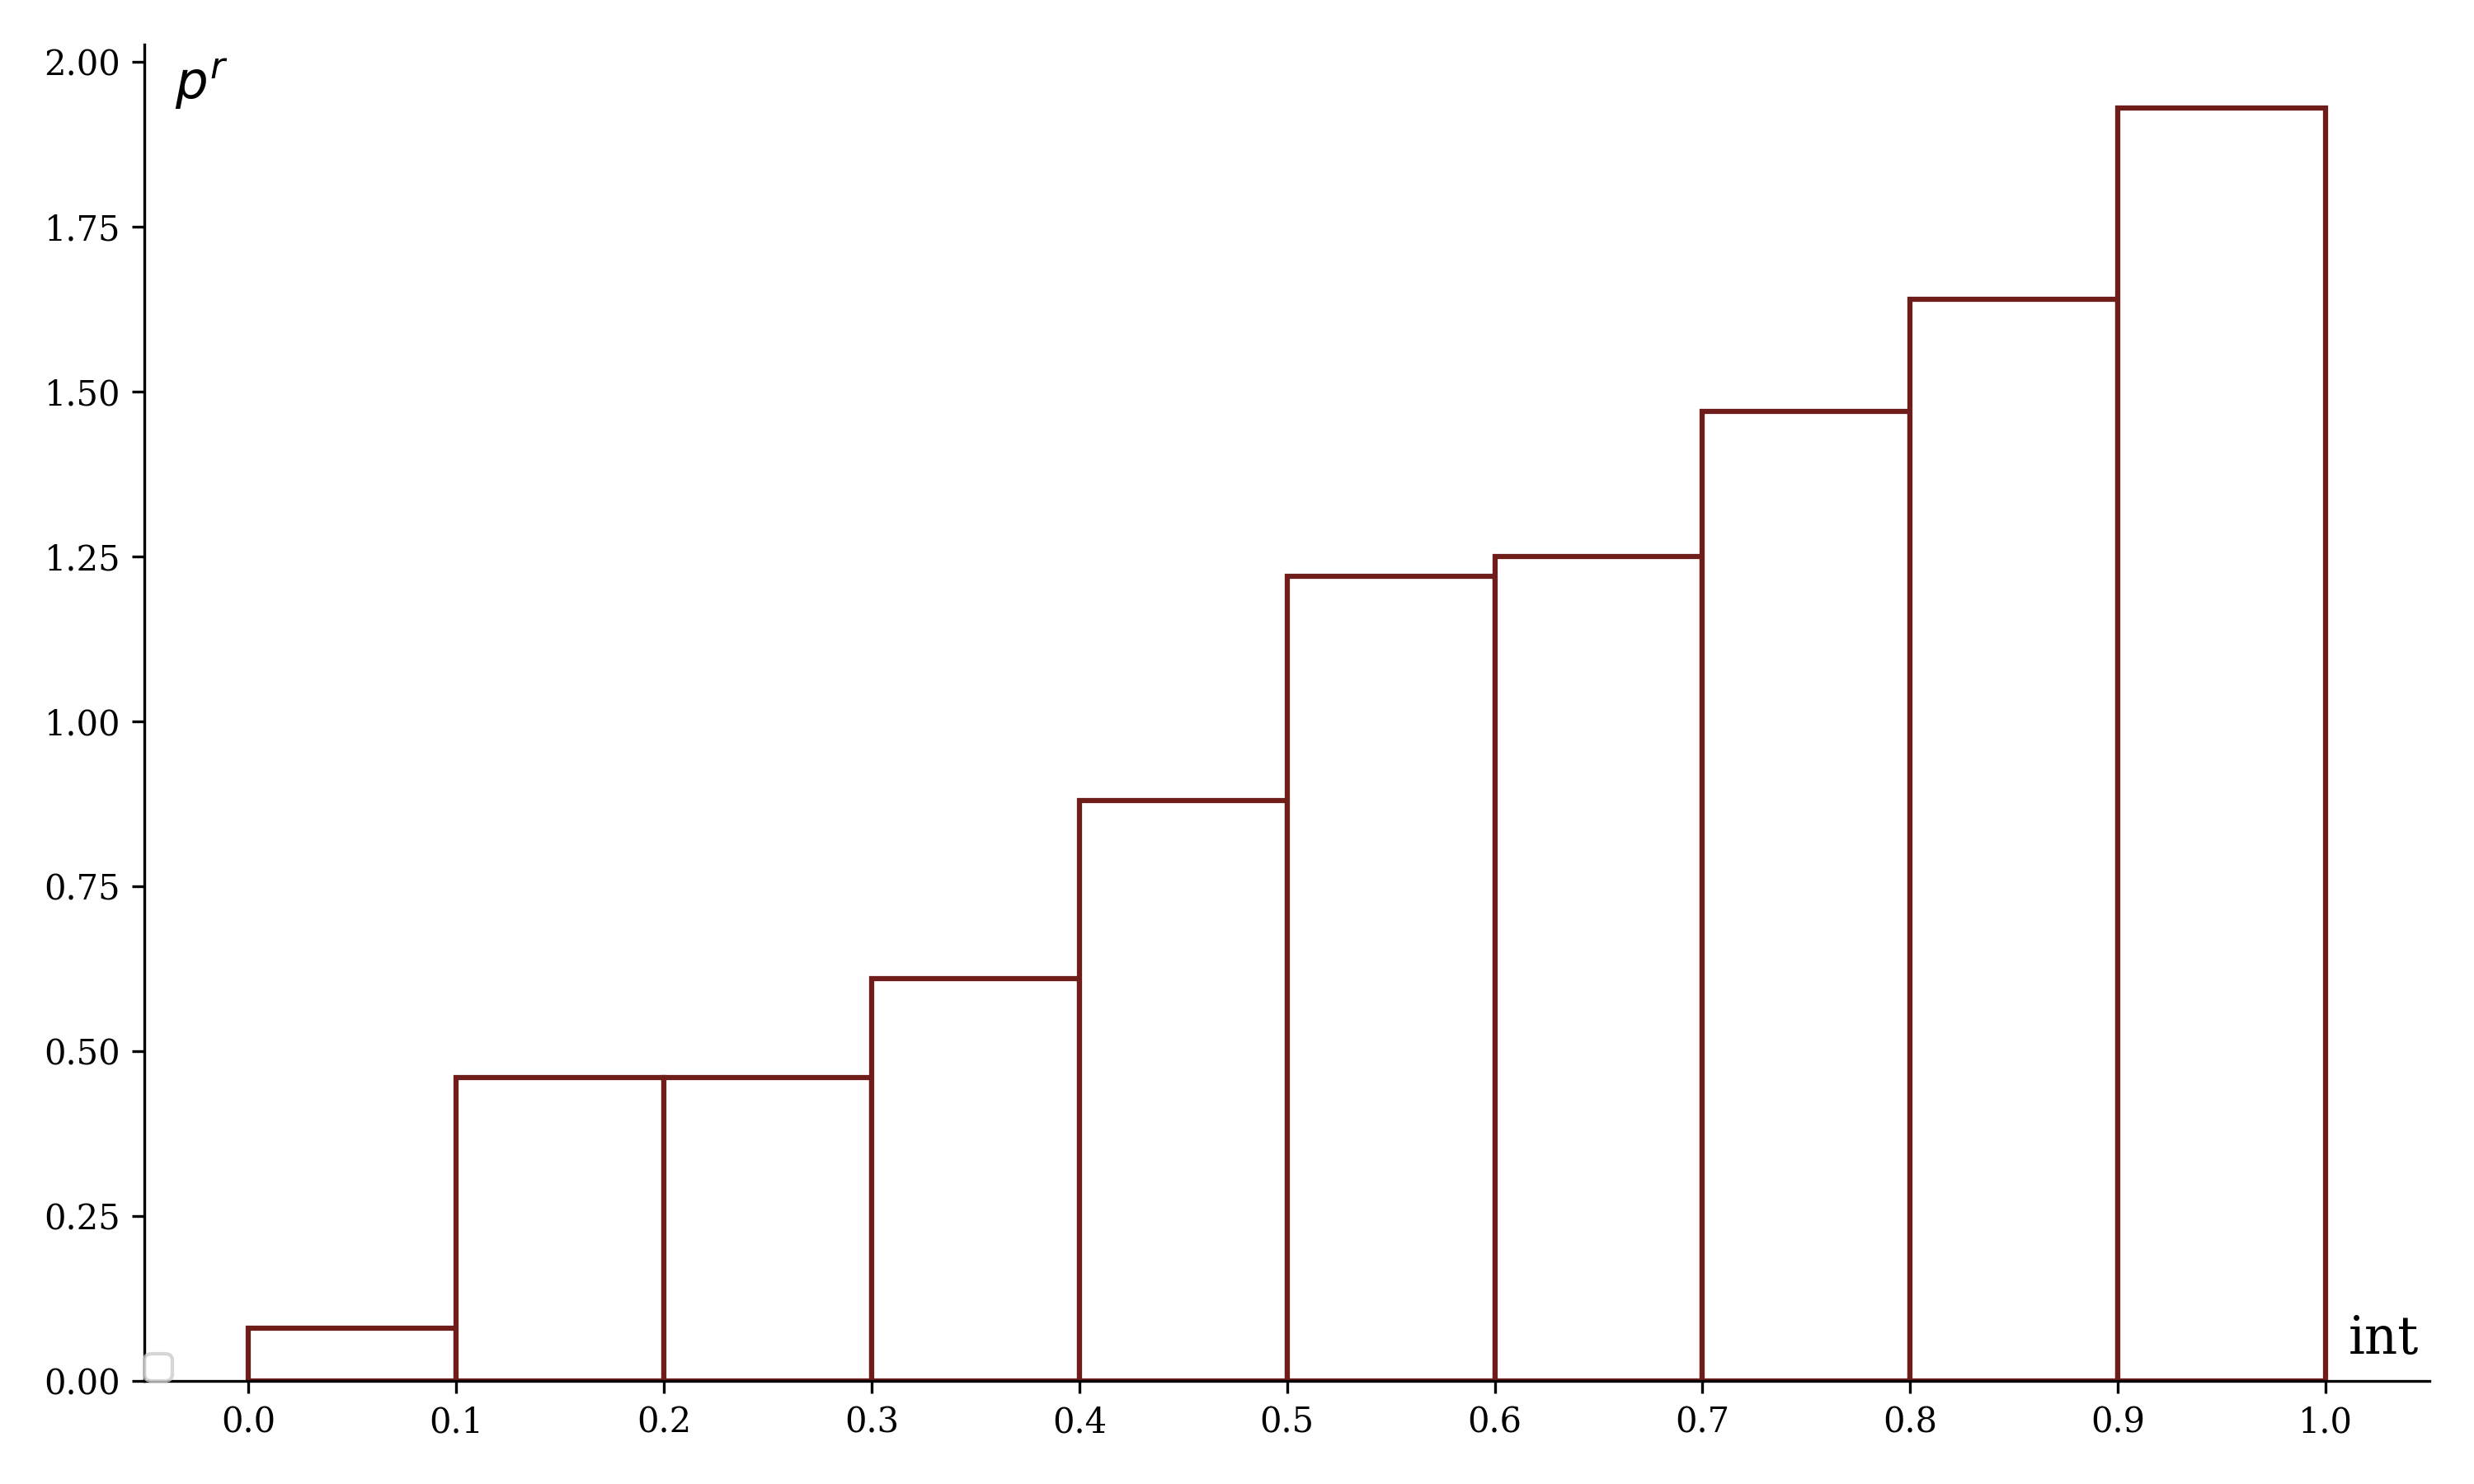
\includegraphics[width=\textwidth, height=\textheight, keepaspectratio]{sample16_hist}
\end{minipage}

\begin{minipage}[t]{0.25\textwidth}
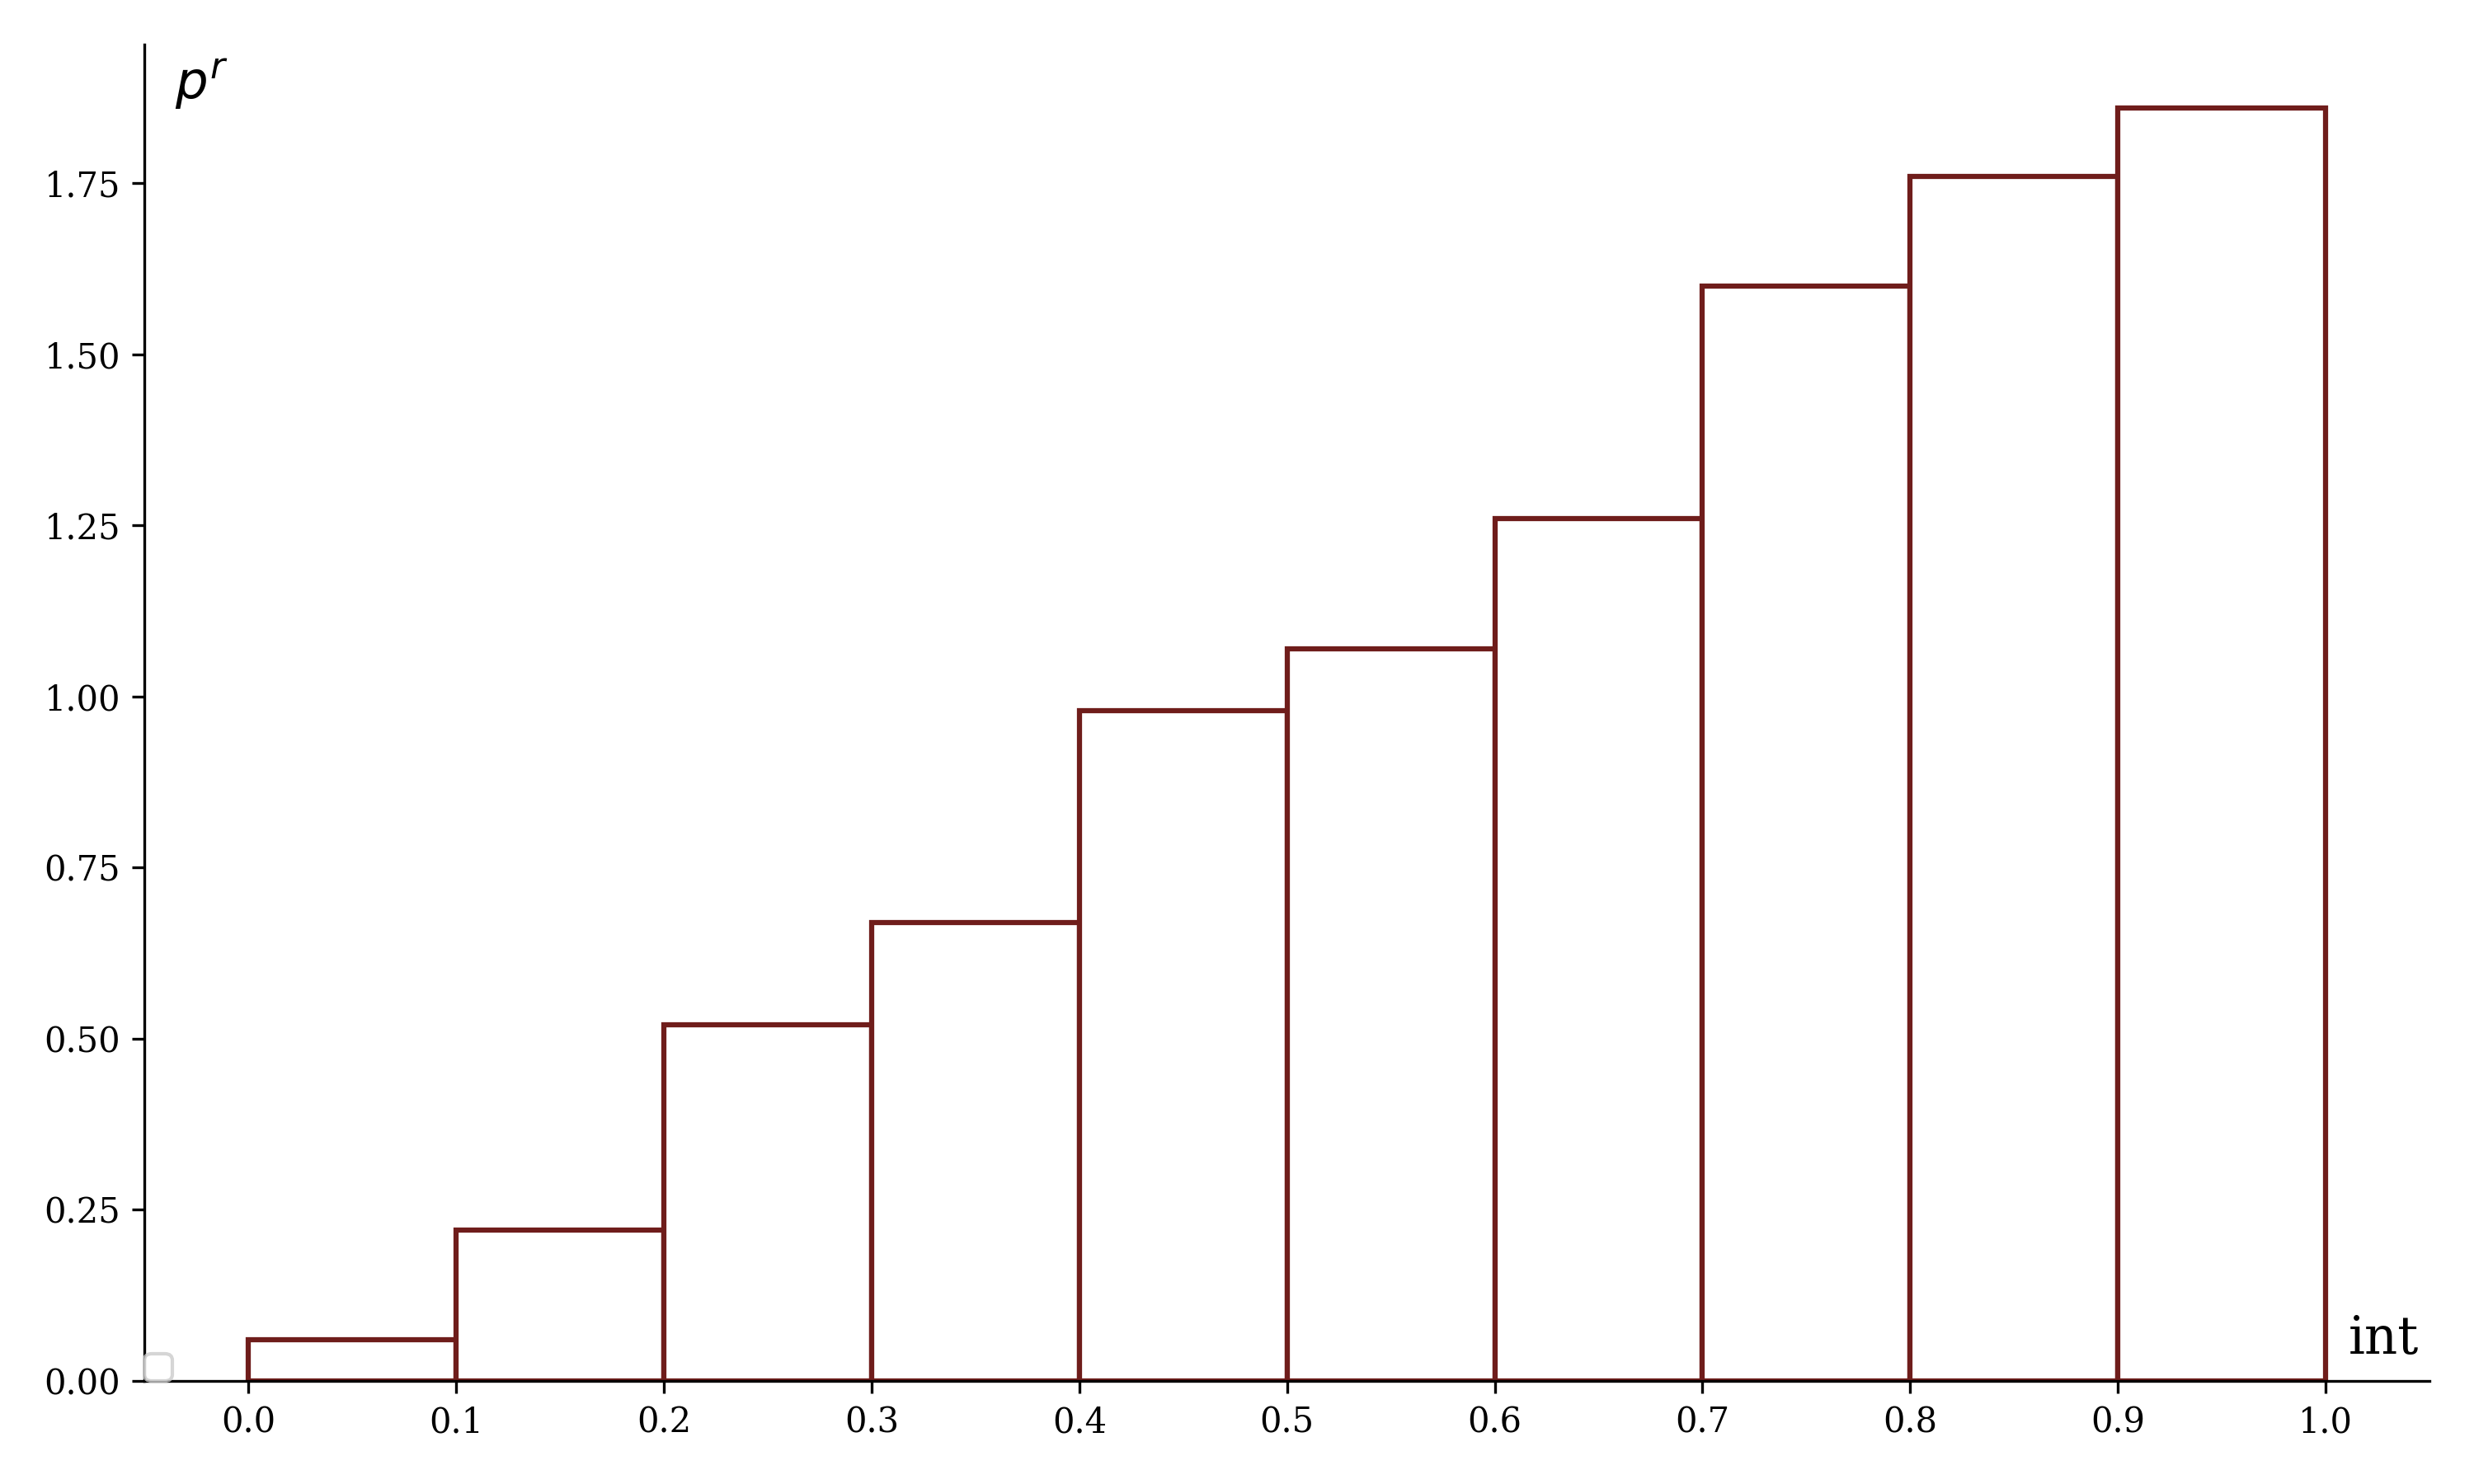
\includegraphics[width=\textwidth, height=\textheight, keepaspectratio]{sample17_hist}
\end{minipage}%
\begin{minipage}[t]{0.25\textwidth}
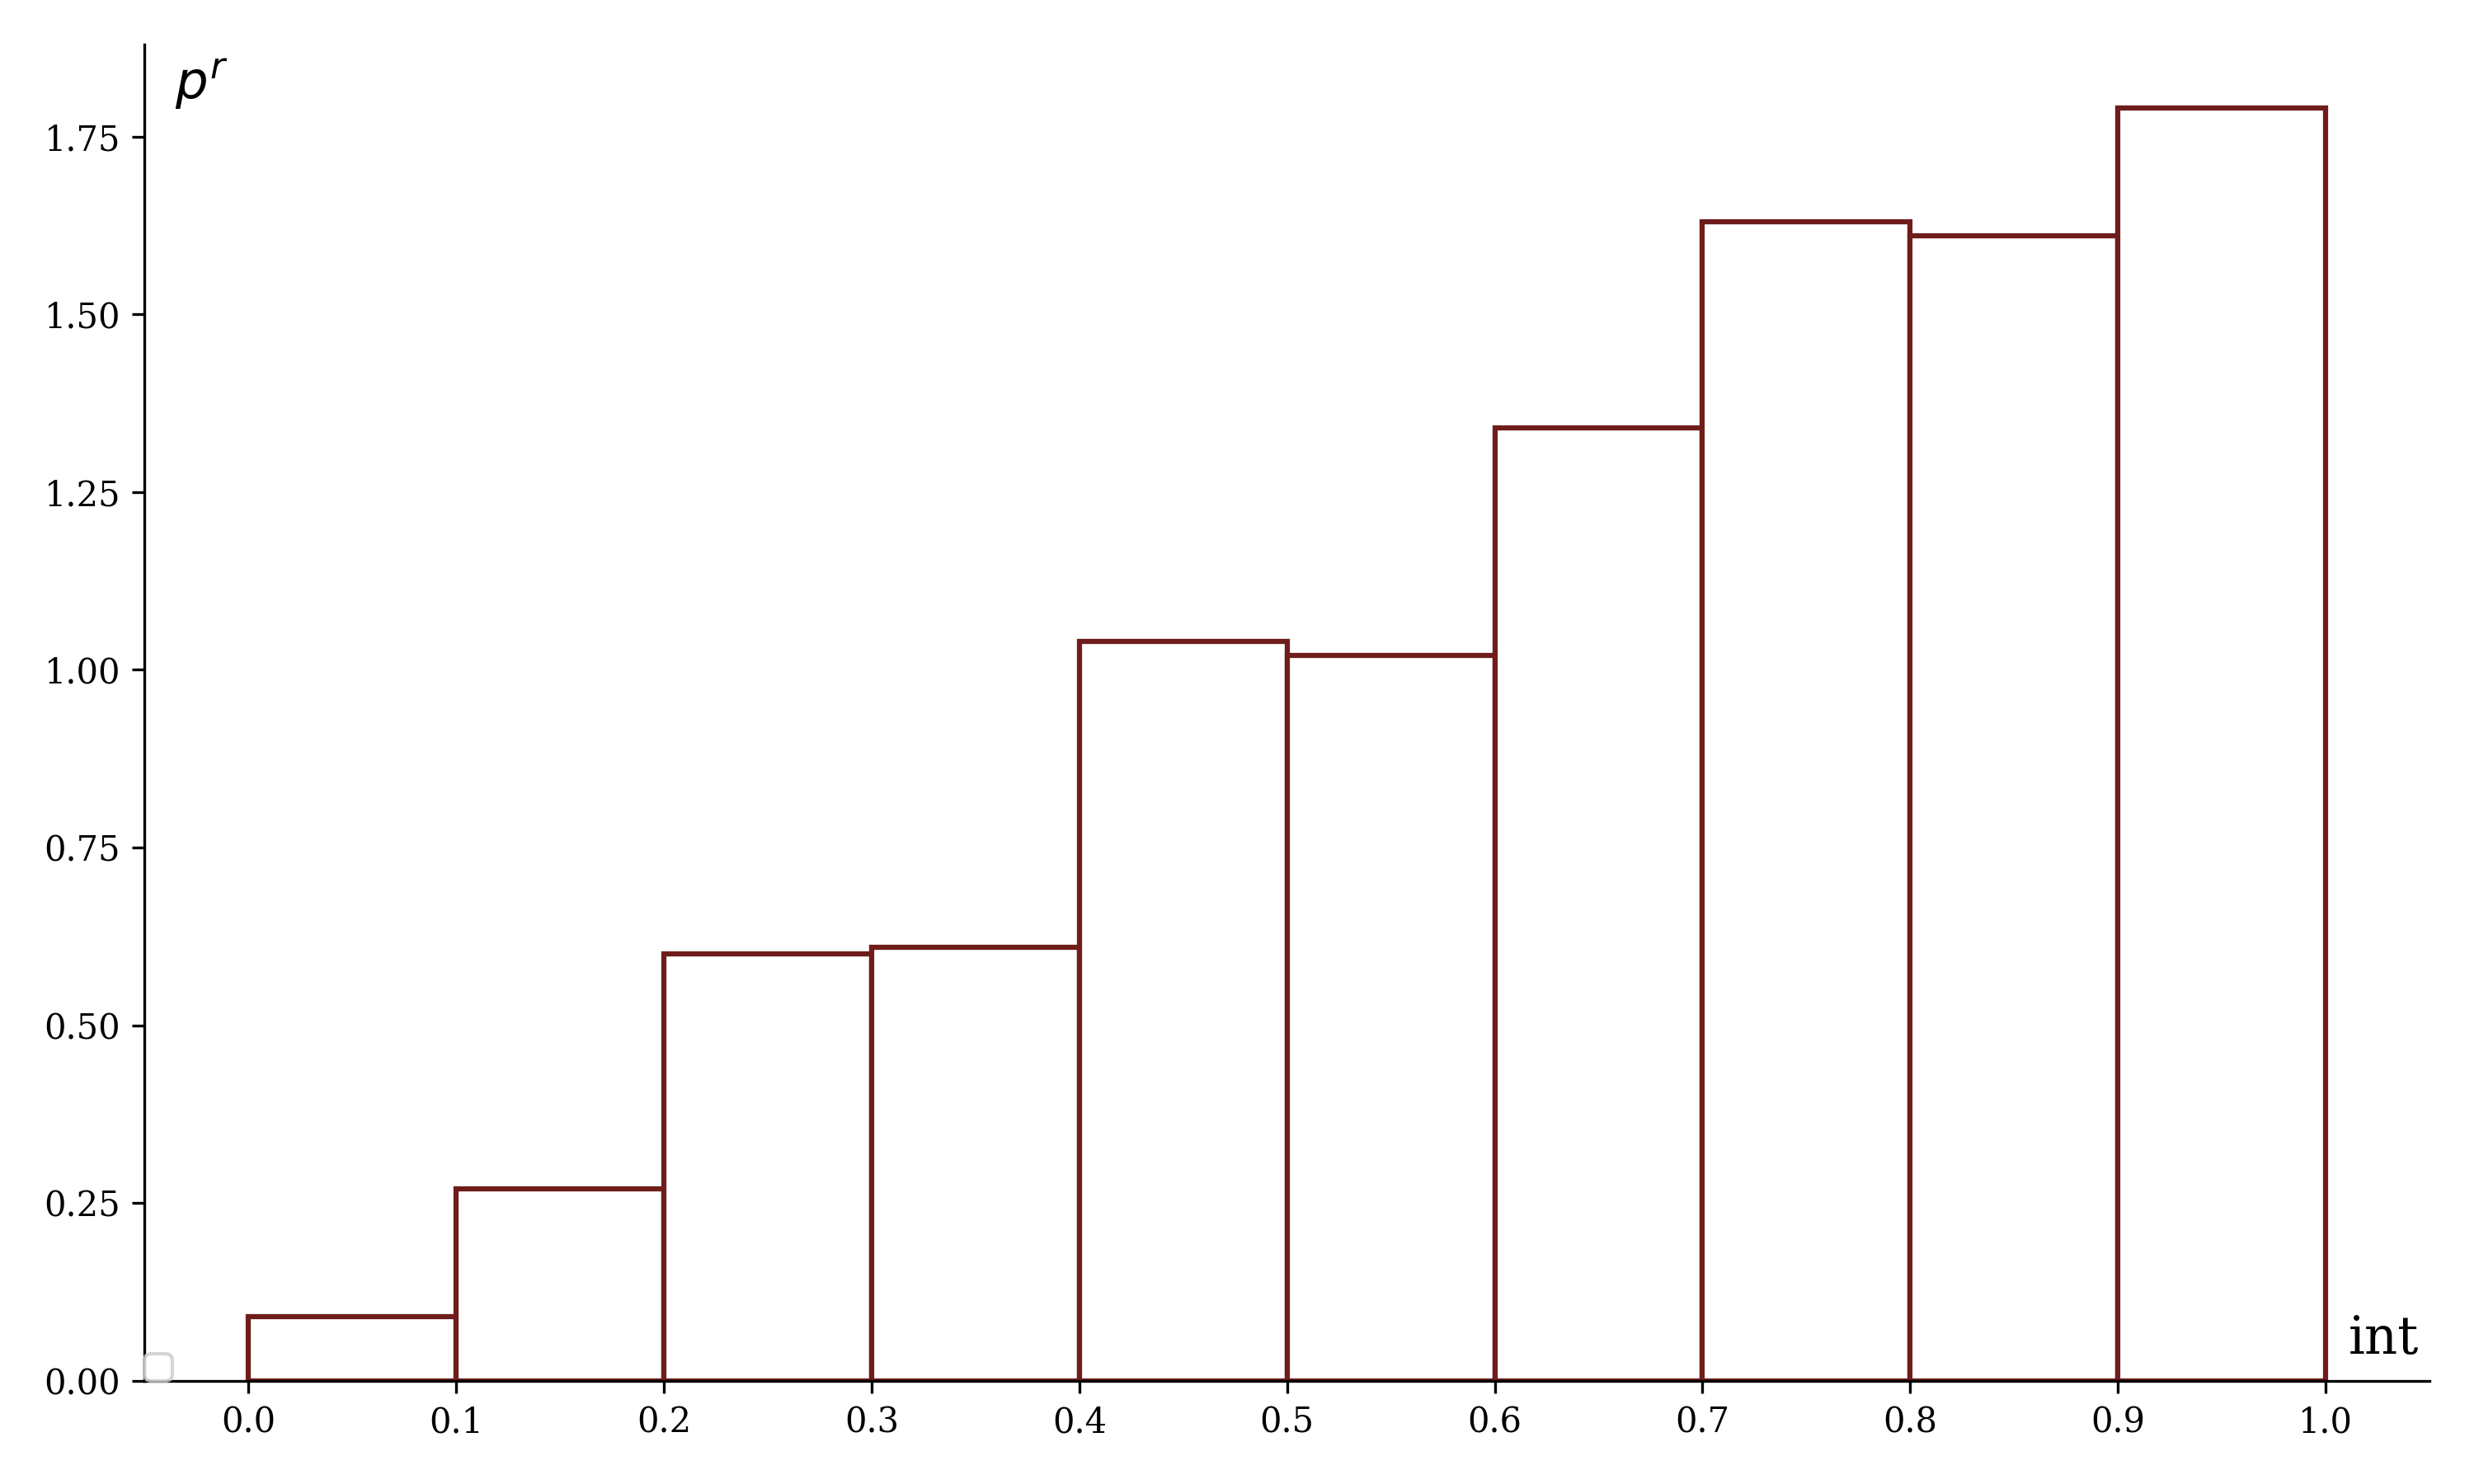
\includegraphics[width=\textwidth, height=\textheight, keepaspectratio]{sample18_hist}
\end{minipage}%
\begin{minipage}[t]{0.25\textwidth}
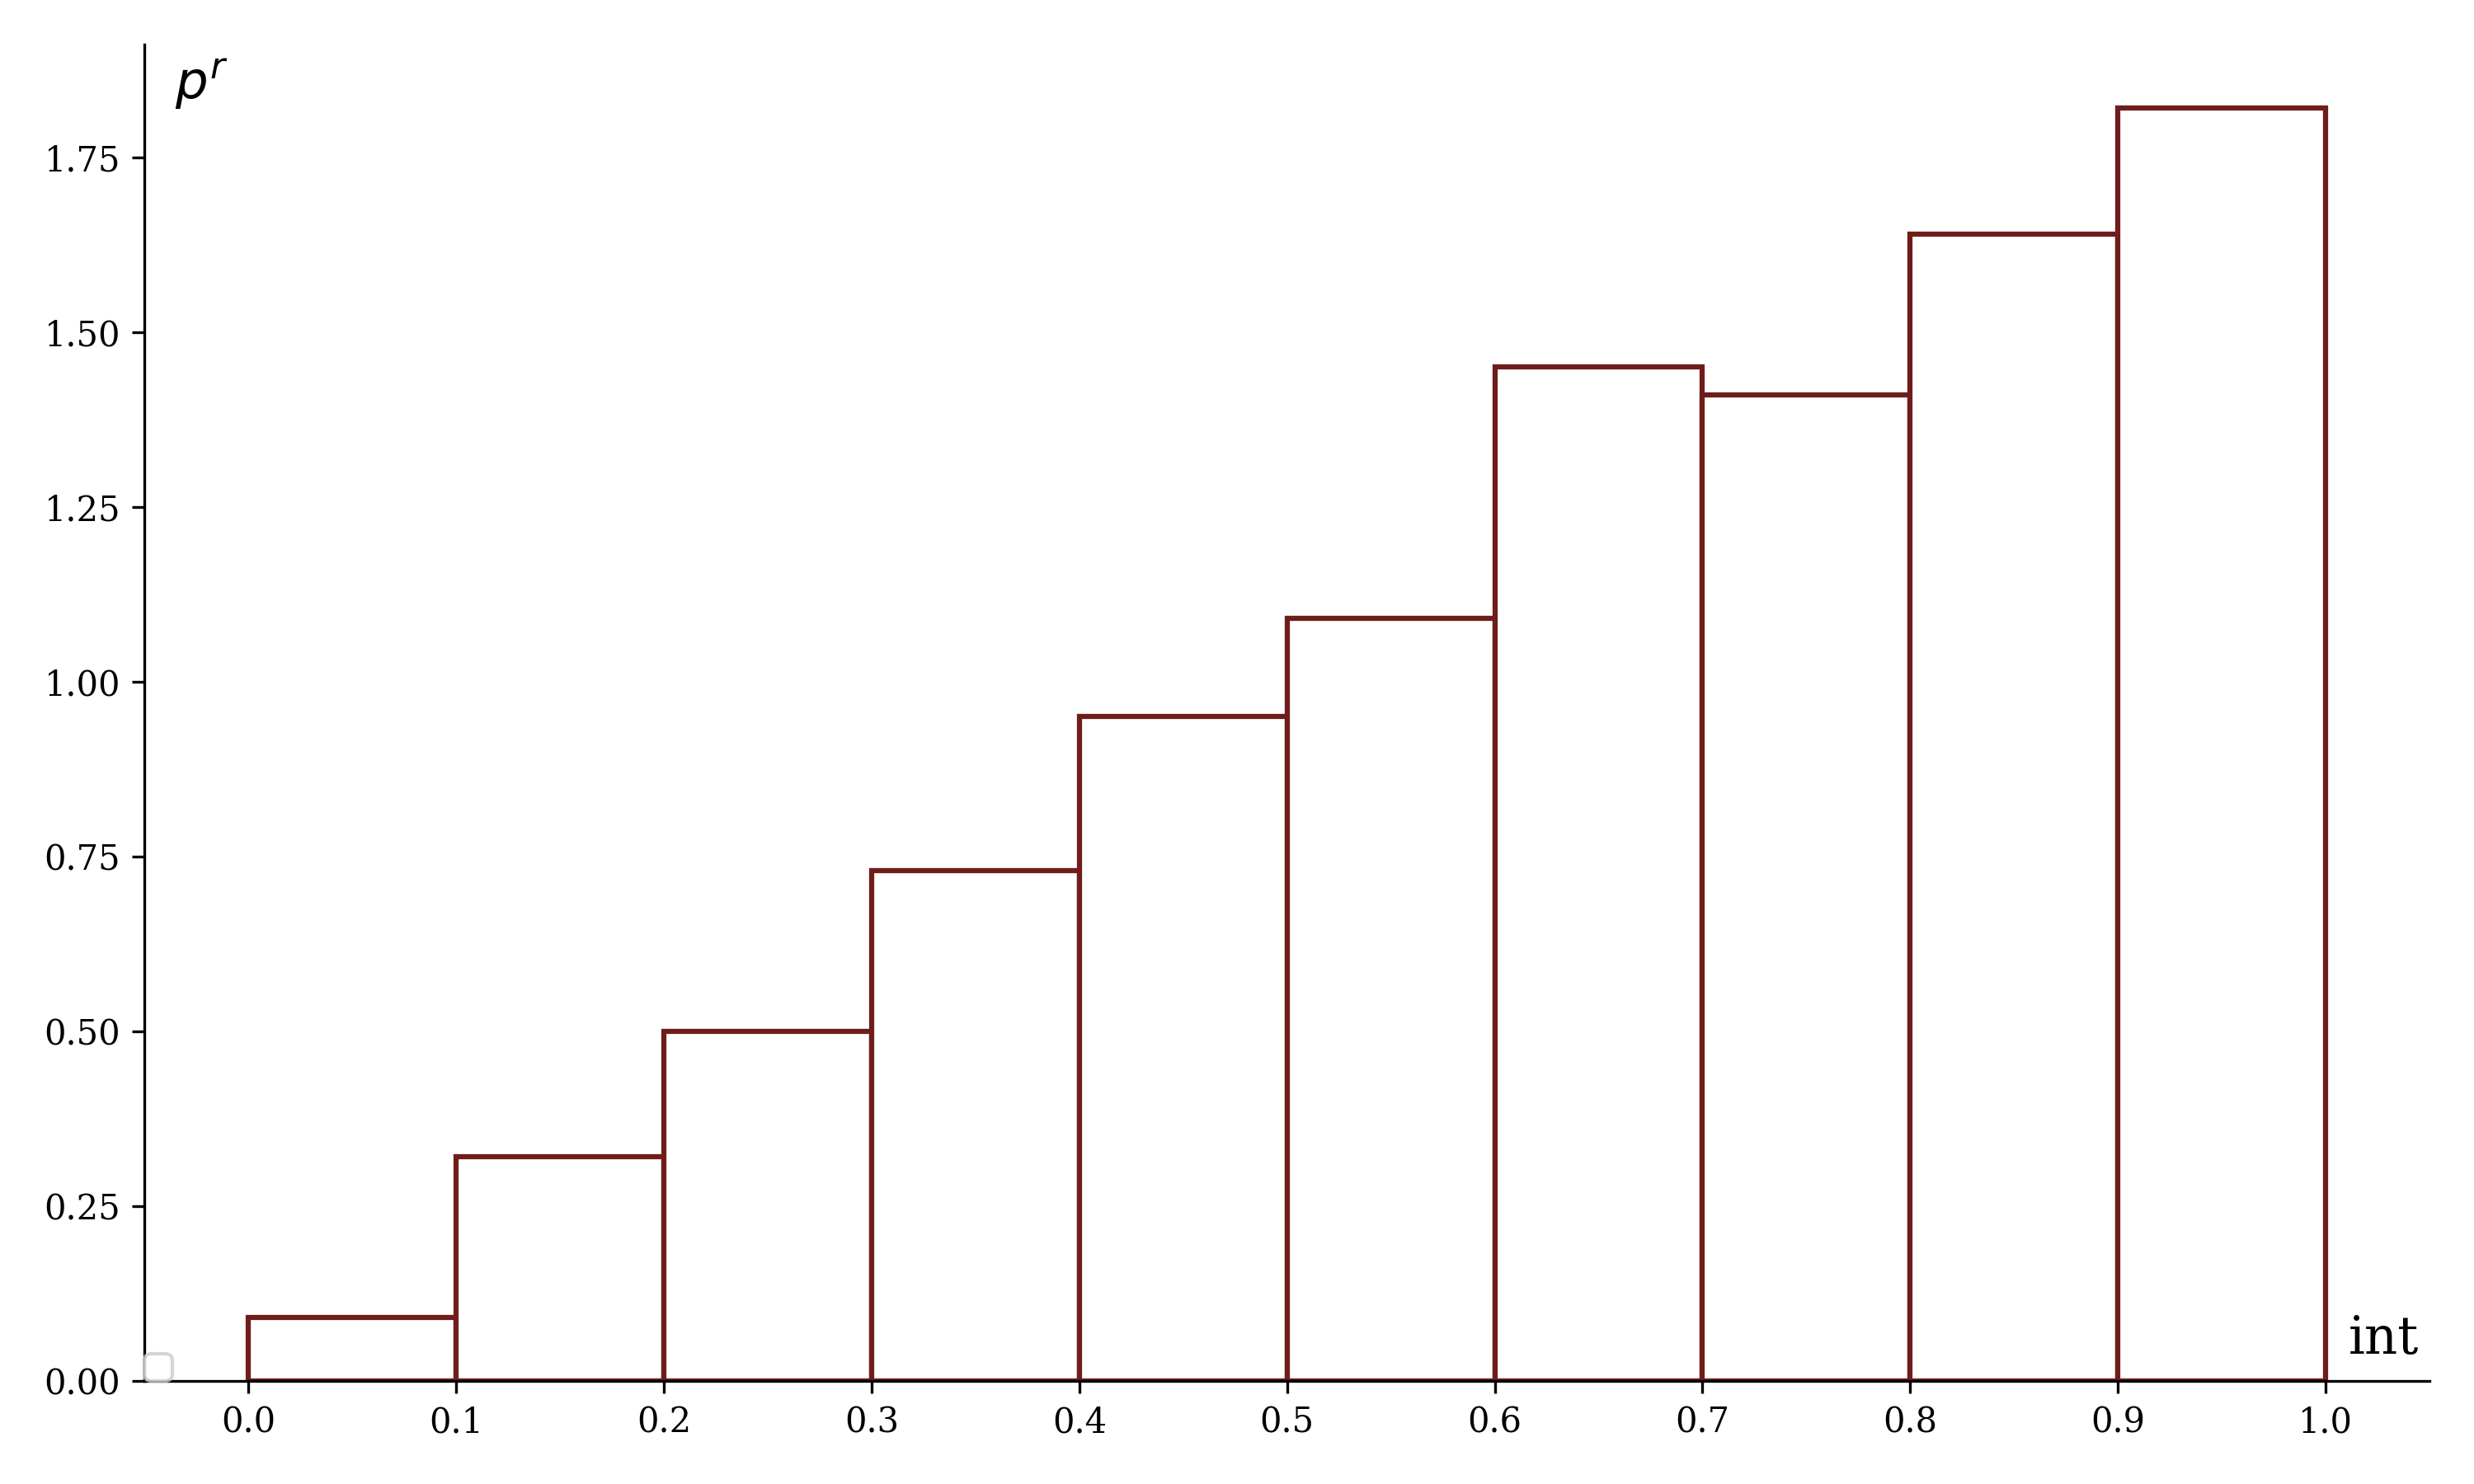
\includegraphics[width=\textwidth, height=\textheight, keepaspectratio]{sample19_hist}
\end{minipage}%
\begin{minipage}[t]{0.25\textwidth}
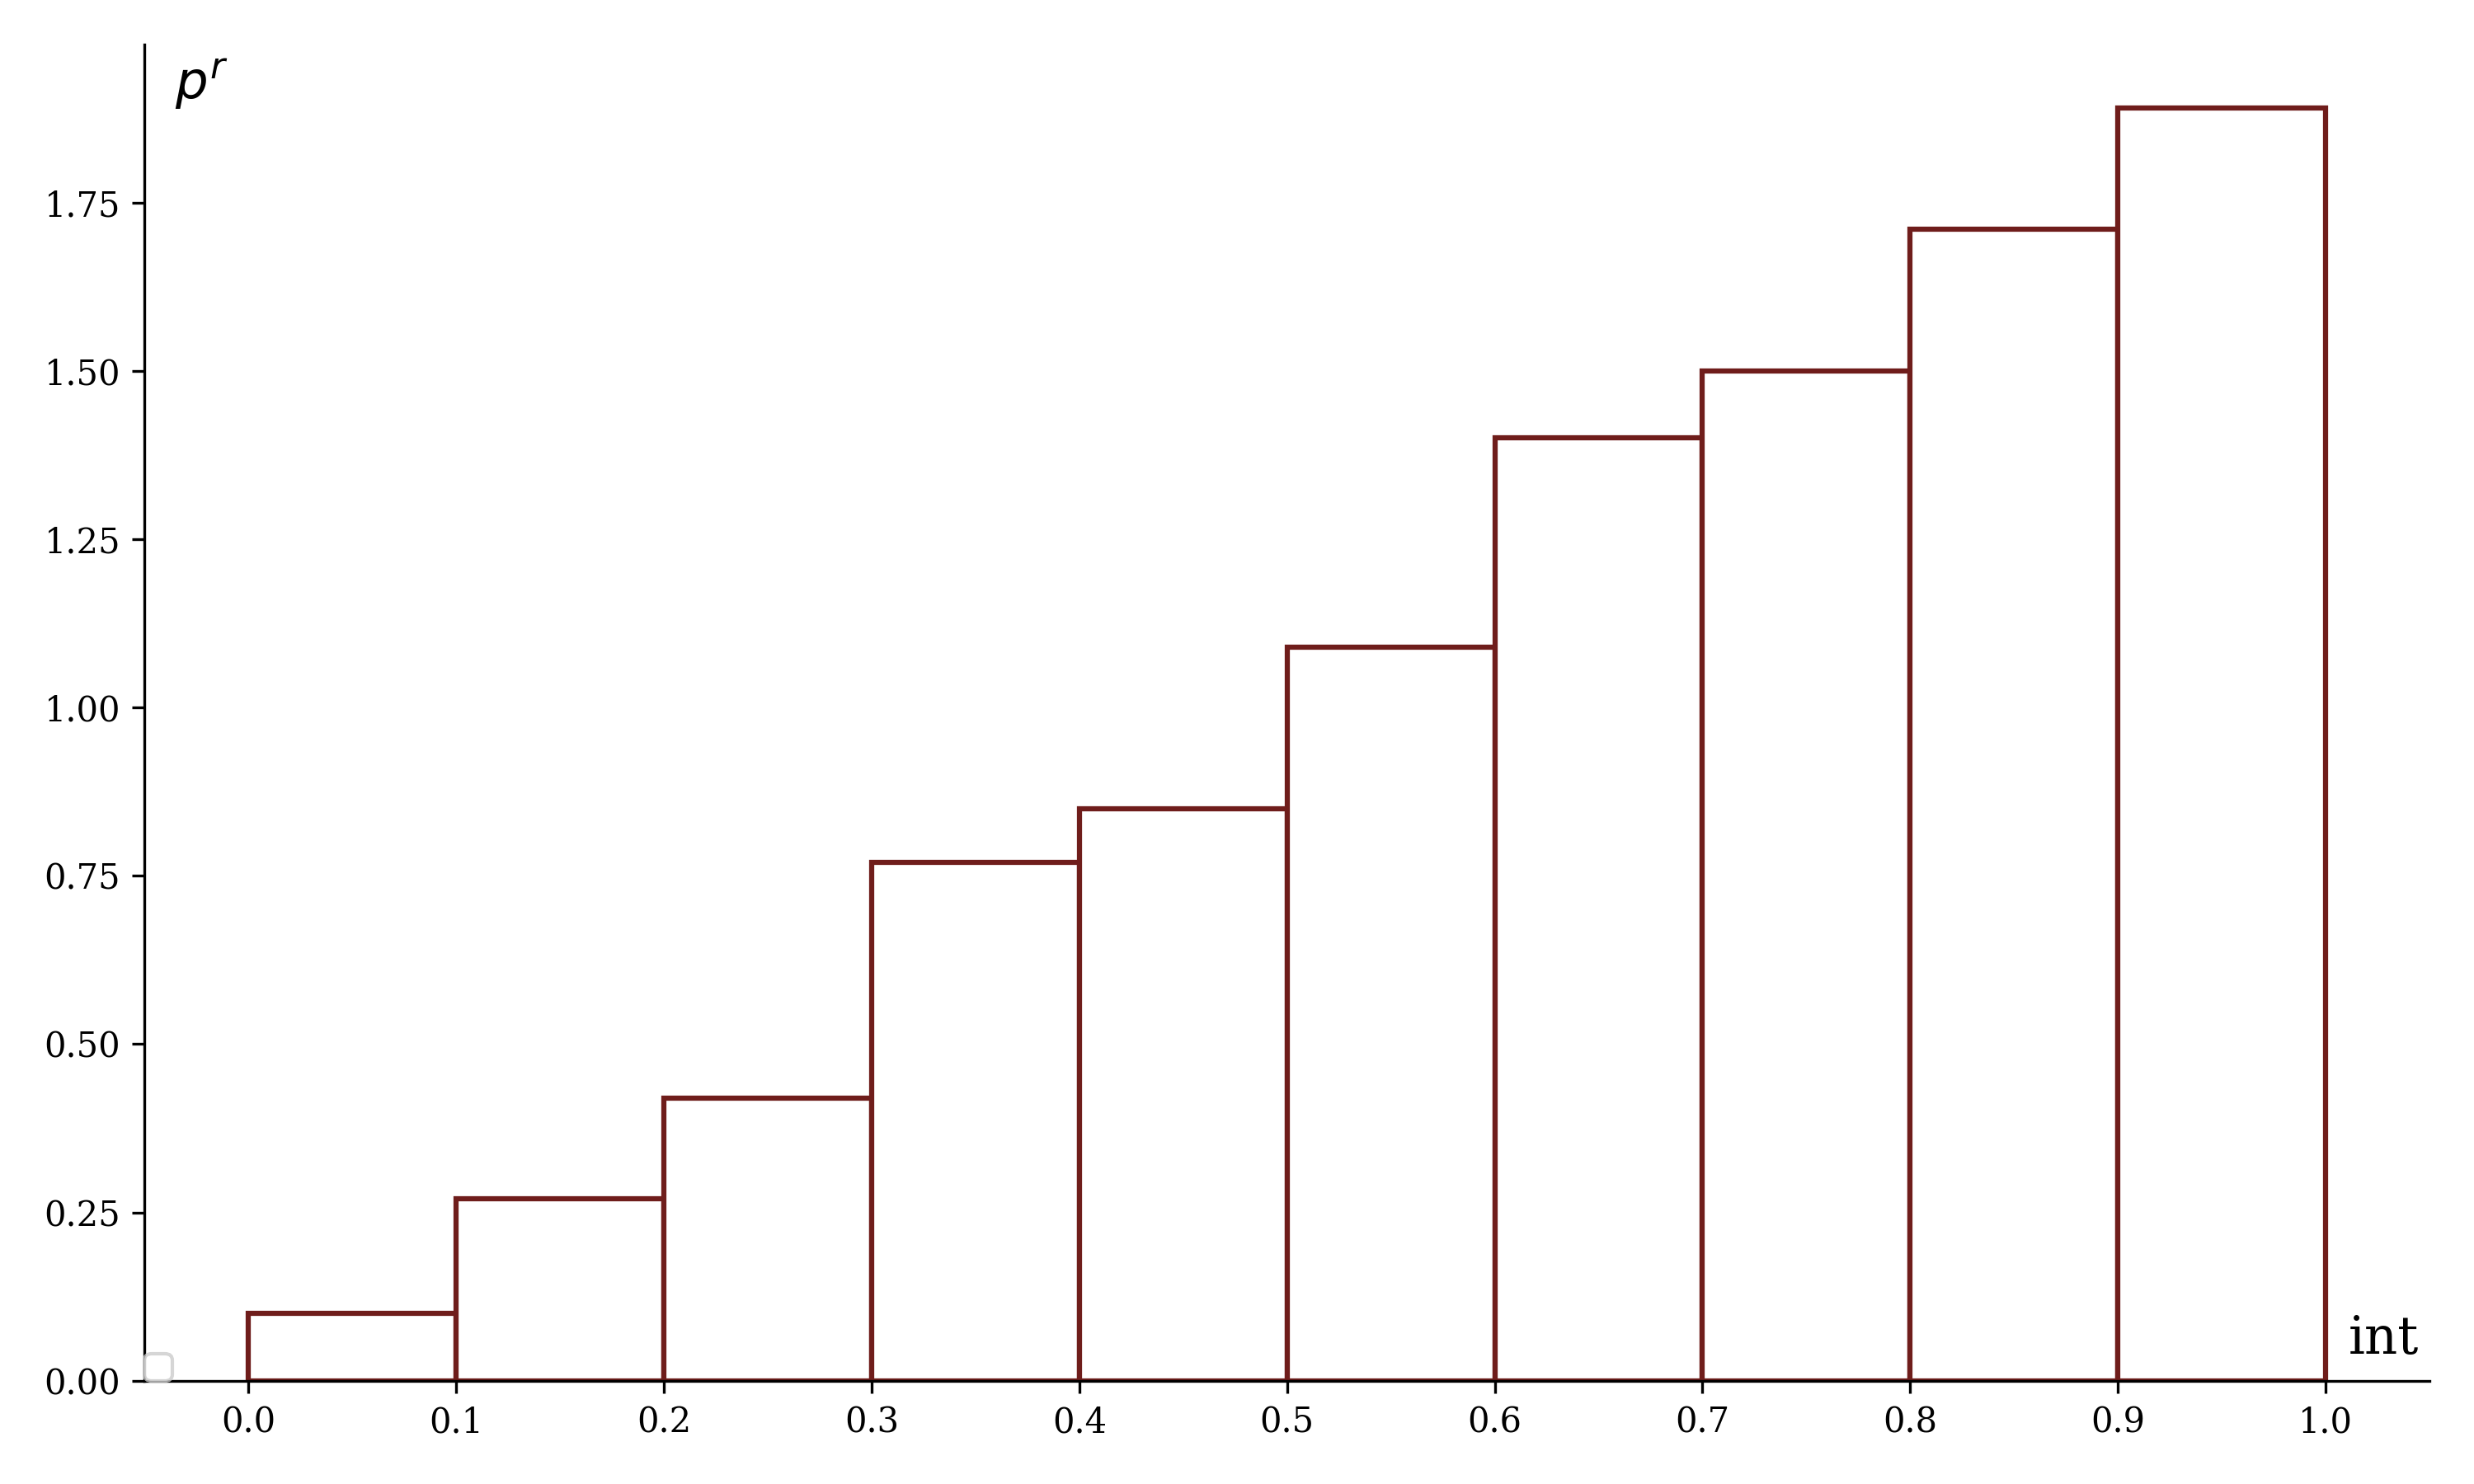
\includegraphics[width=\textwidth, height=\textheight, keepaspectratio]{sample20_hist}
\end{minipage}

\begin{minipage}[t]{0.25\textwidth}
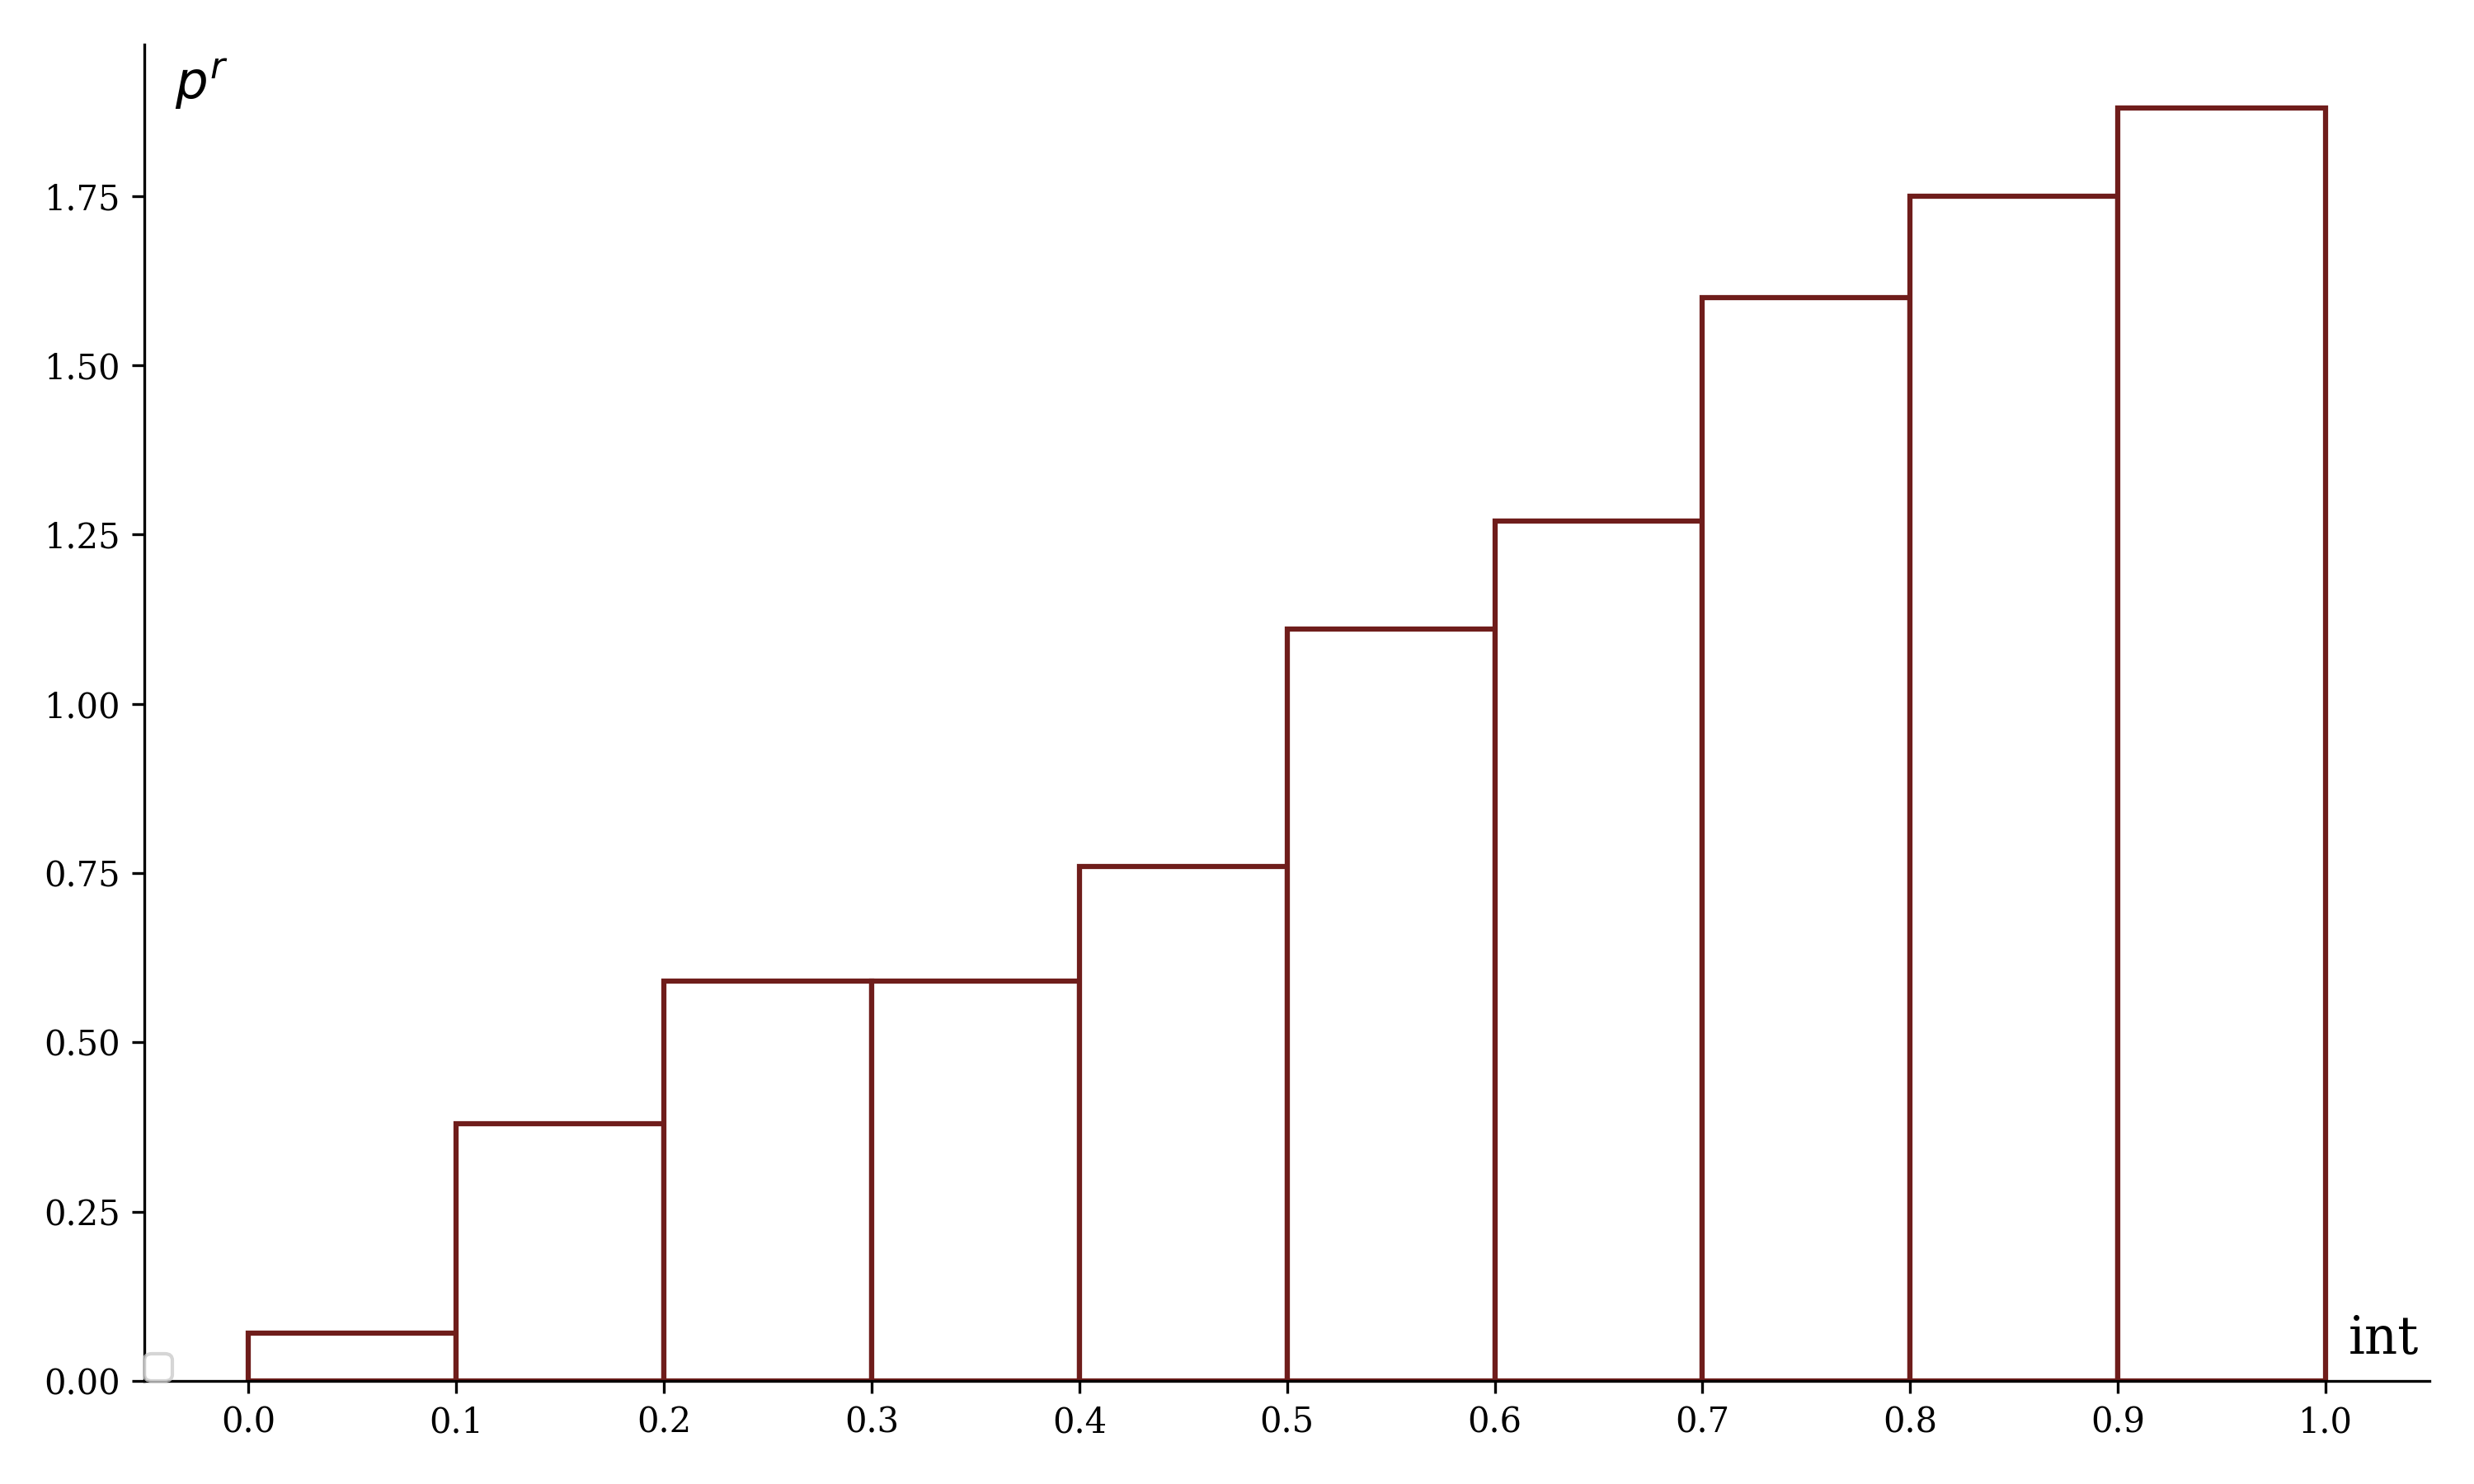
\includegraphics[width=\textwidth, height=\textheight, keepaspectratio]{sample21_hist}
\end{minipage}%
\begin{minipage}[t]{0.25\textwidth}
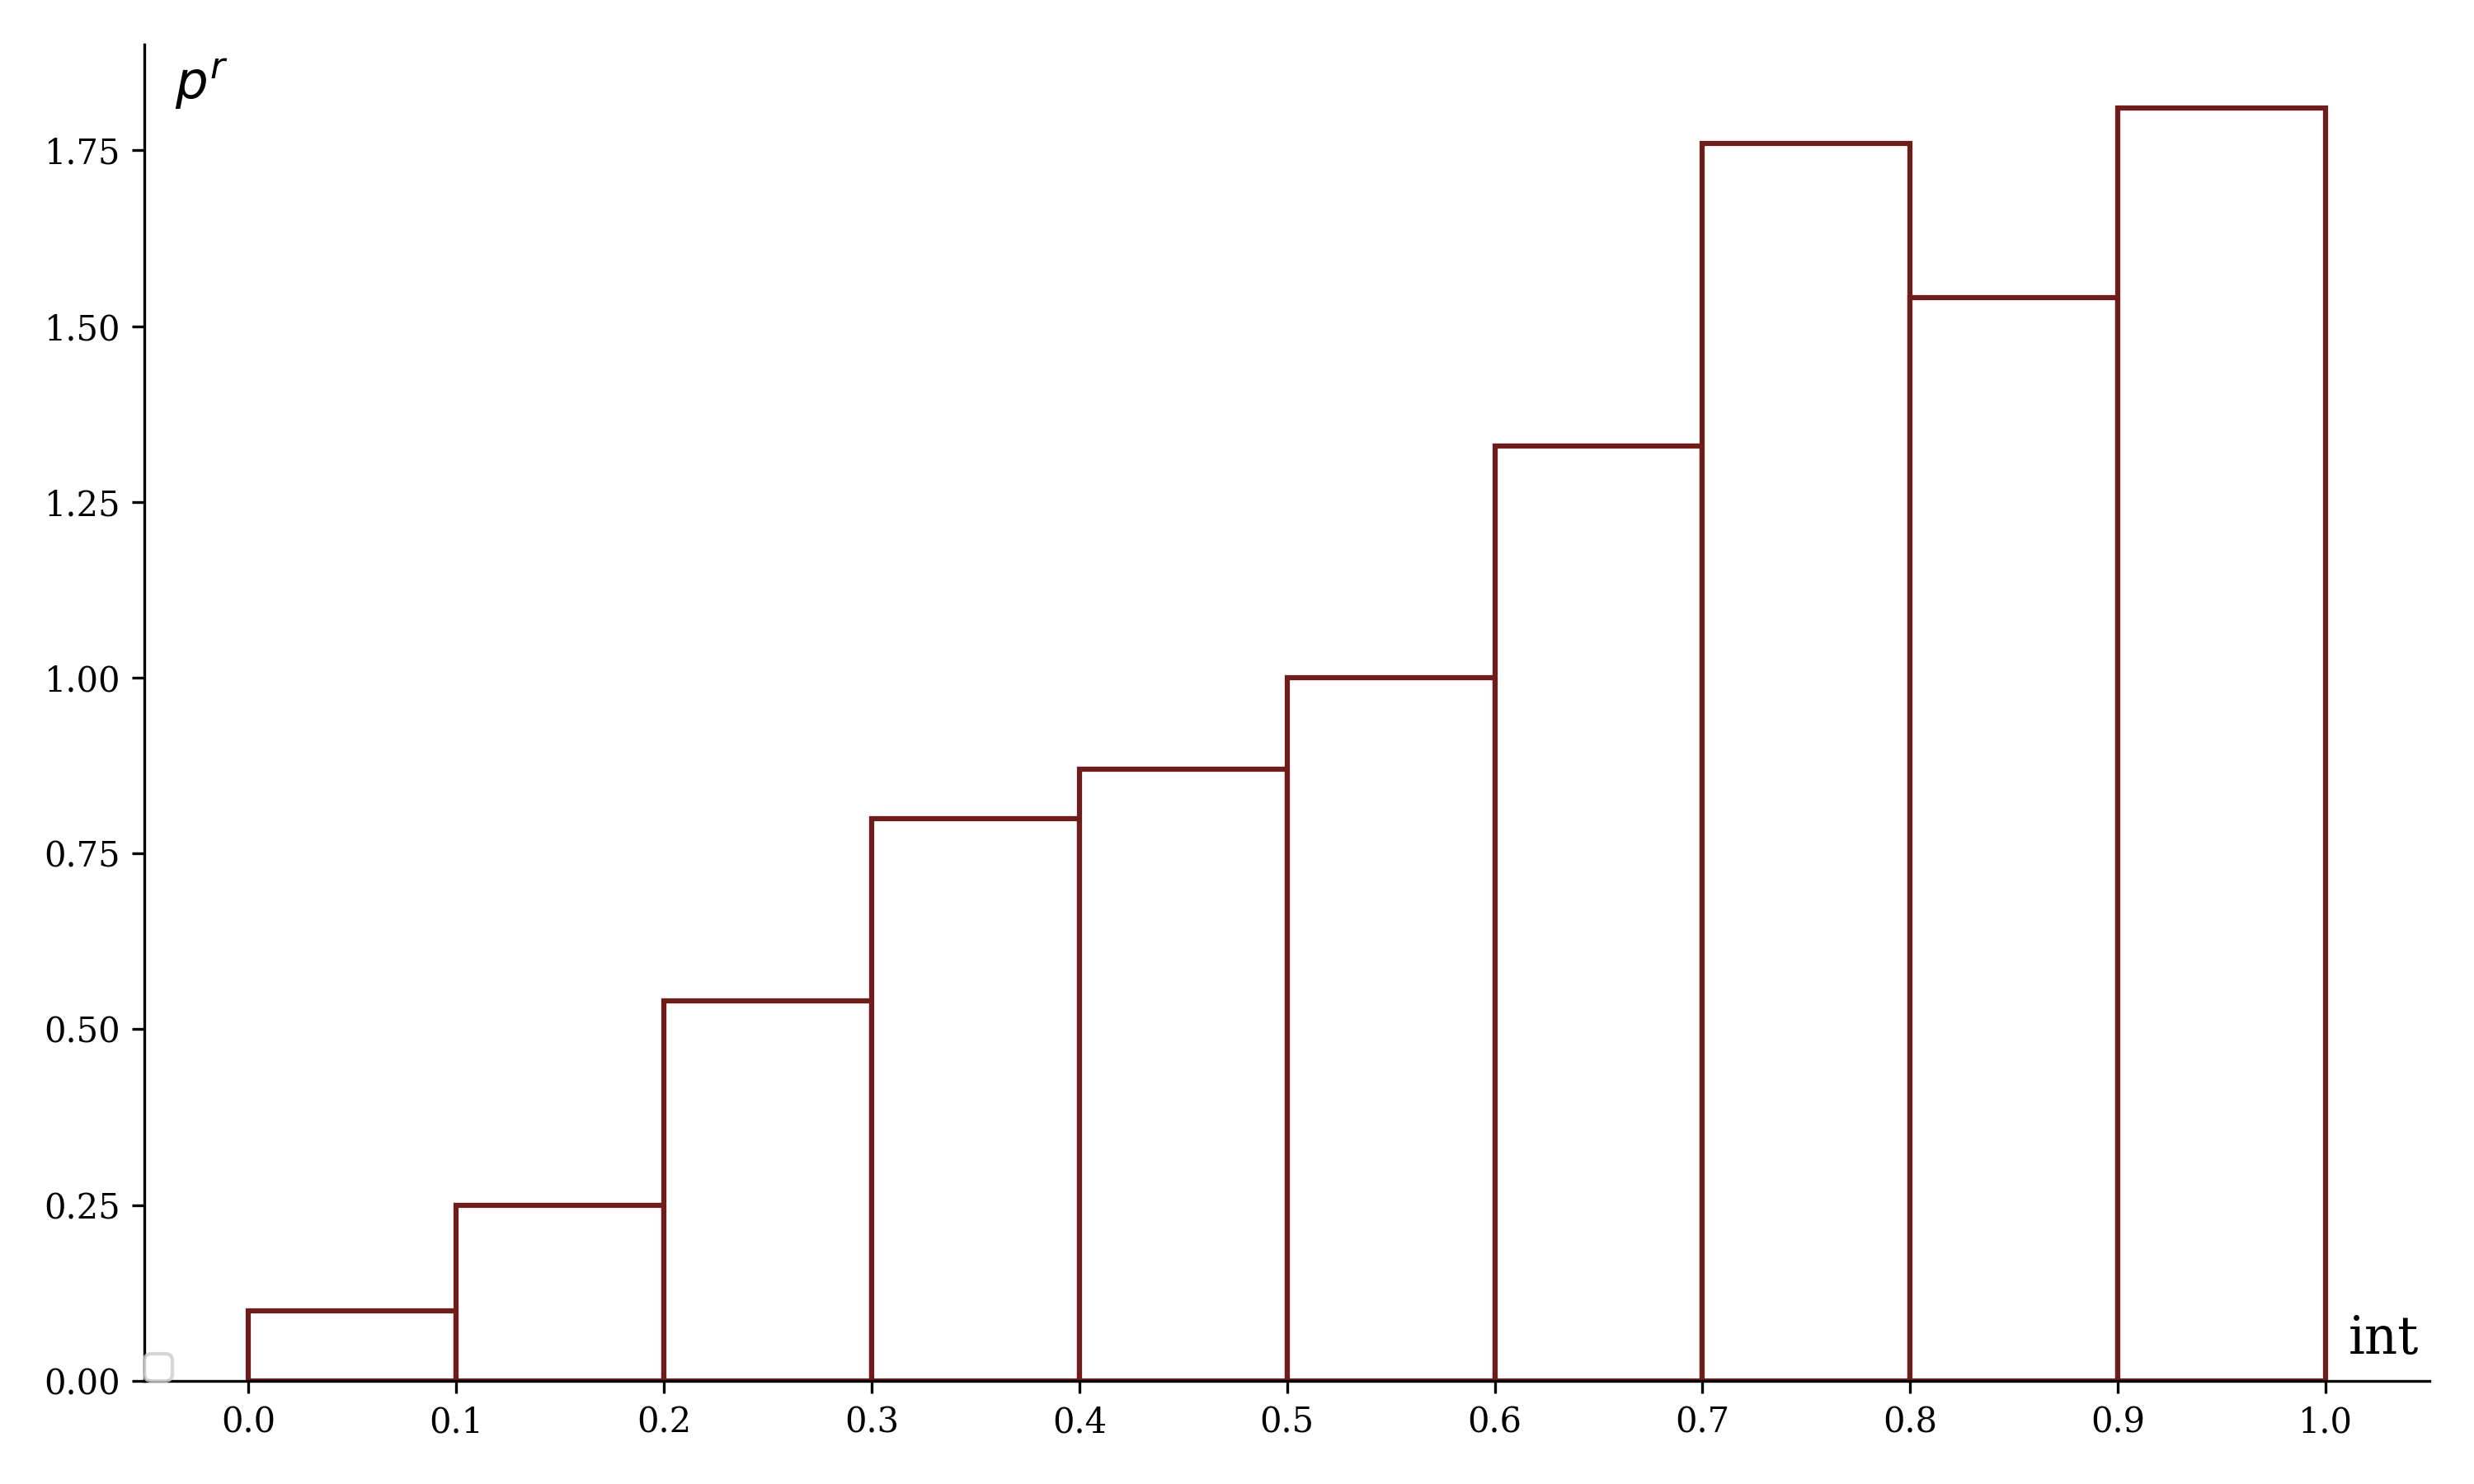
\includegraphics[width=\textwidth, height=\textheight, keepaspectratio]{sample22_hist}
\end{minipage}%
\begin{minipage}[t]{0.25\textwidth}
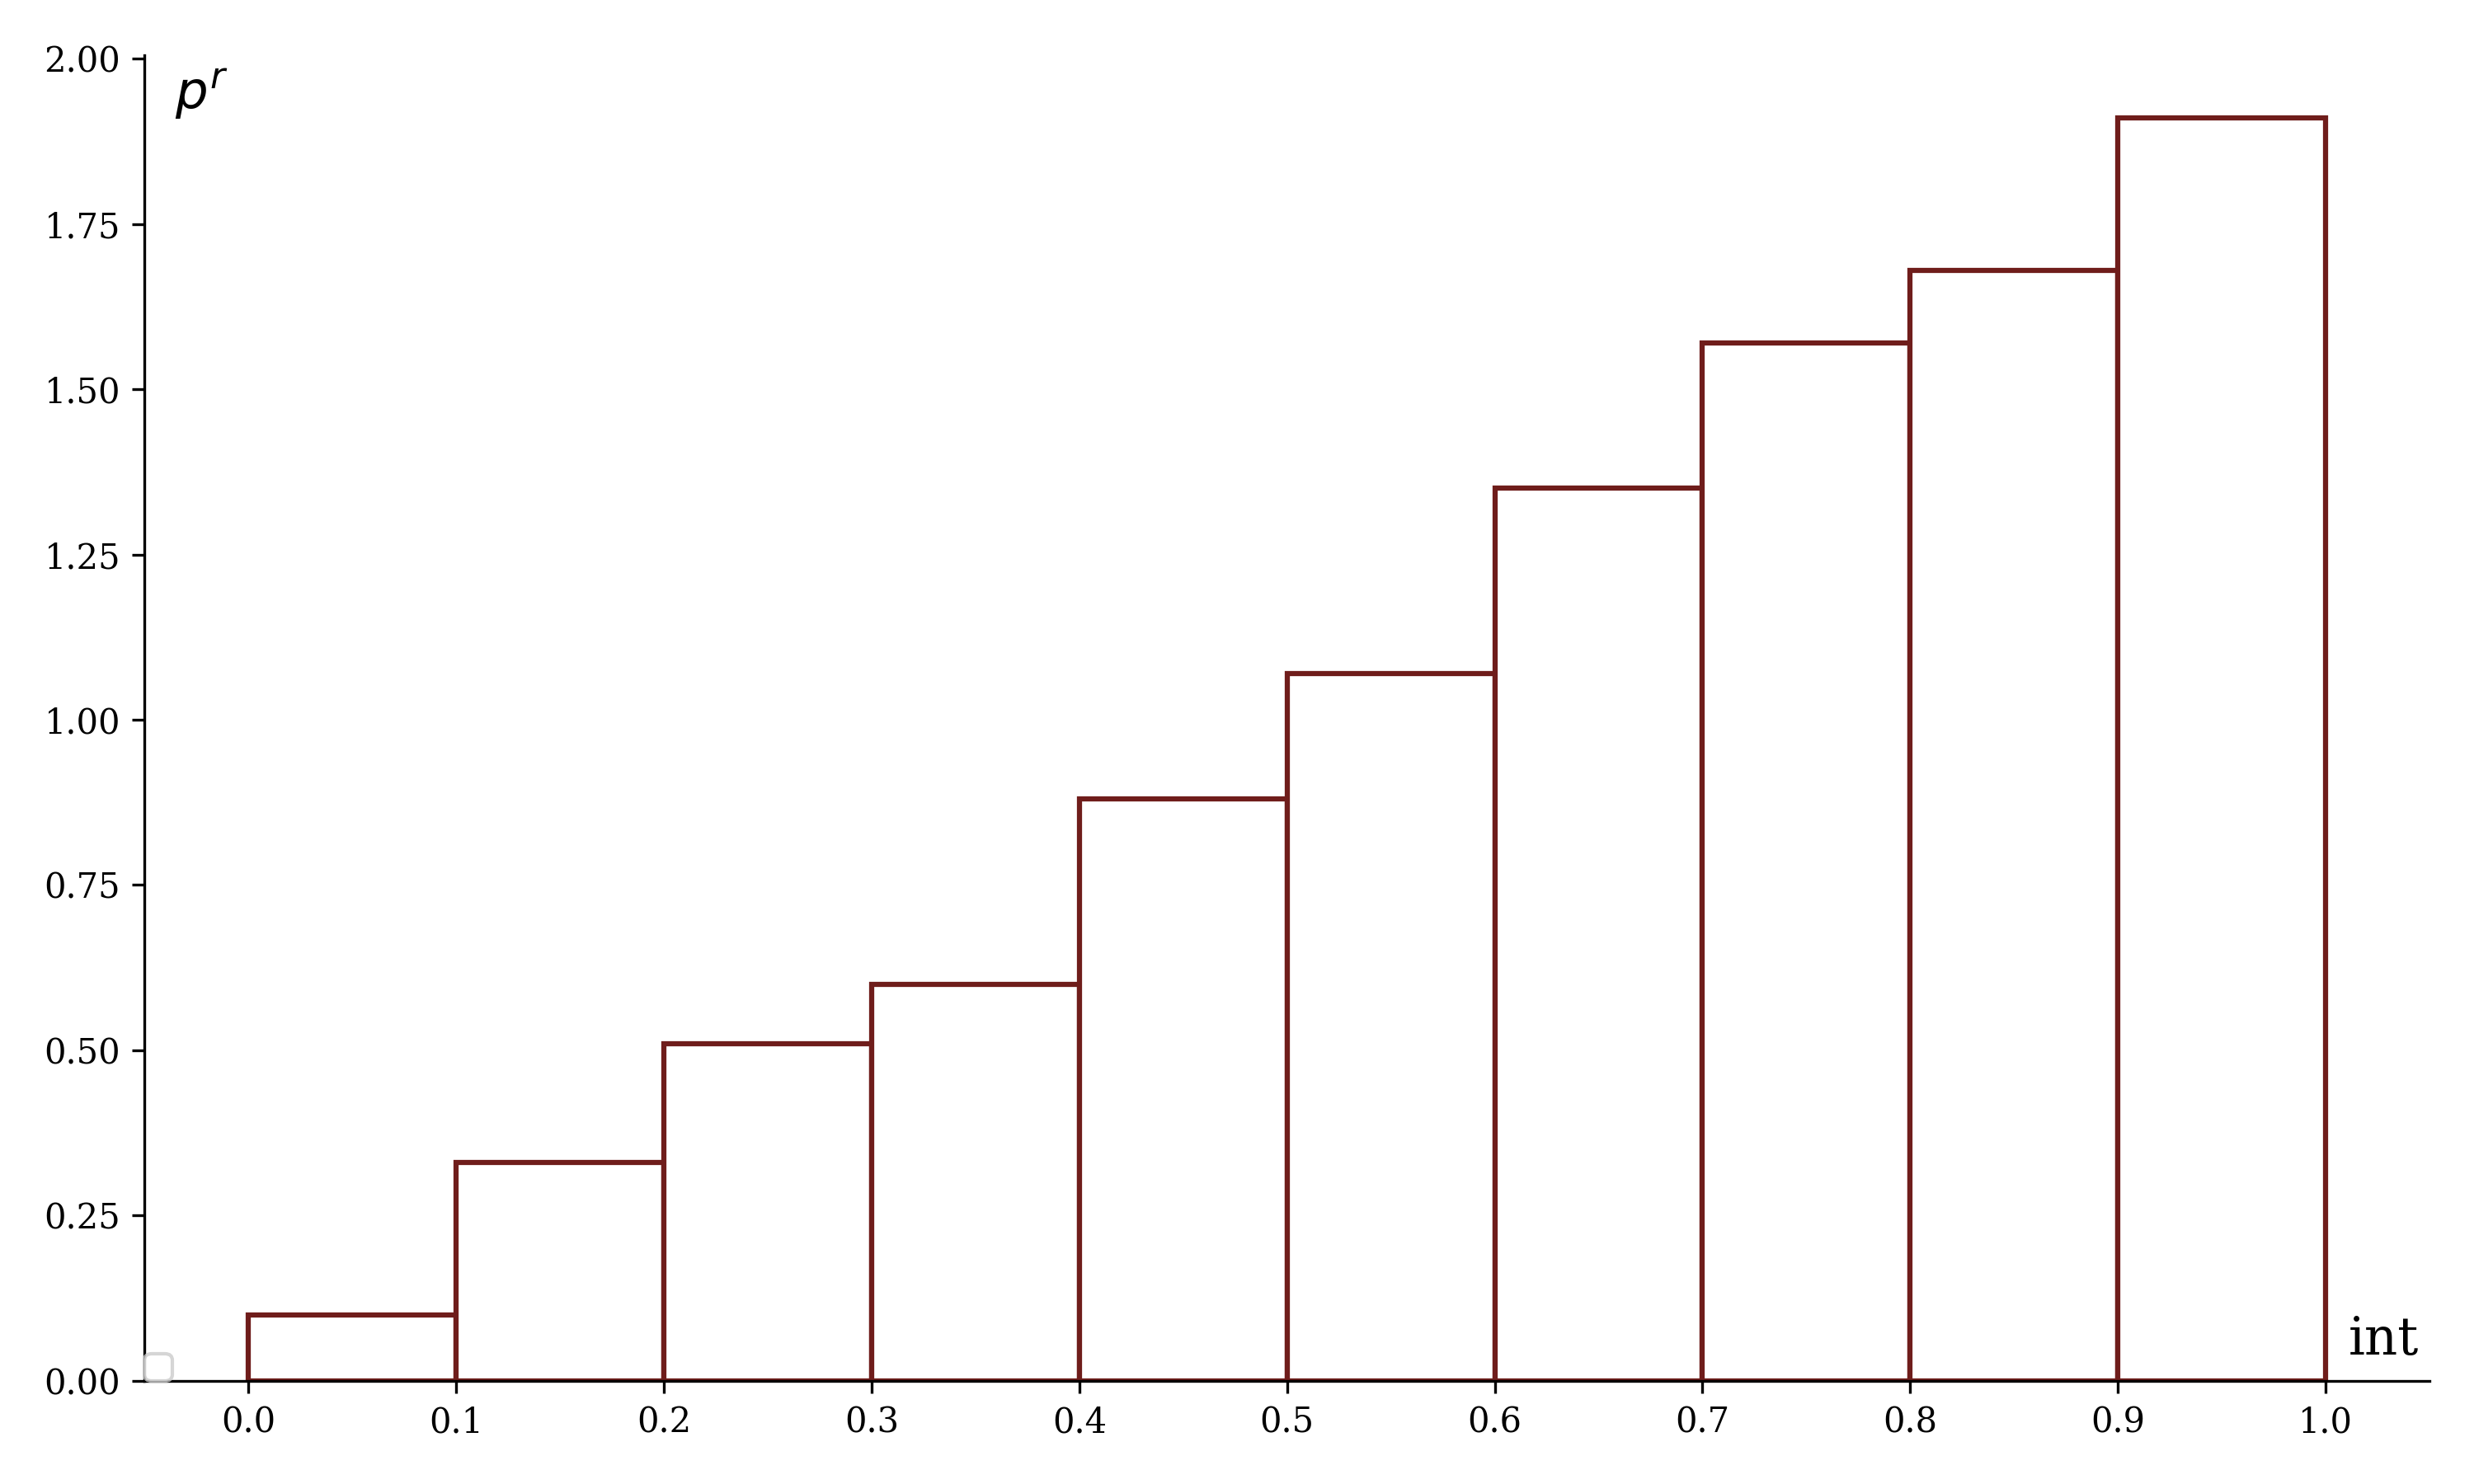
\includegraphics[width=\textwidth, height=\textheight, keepaspectratio]{sample23_hist}
\end{minipage}%
\begin{minipage}[t]{0.25\textwidth}
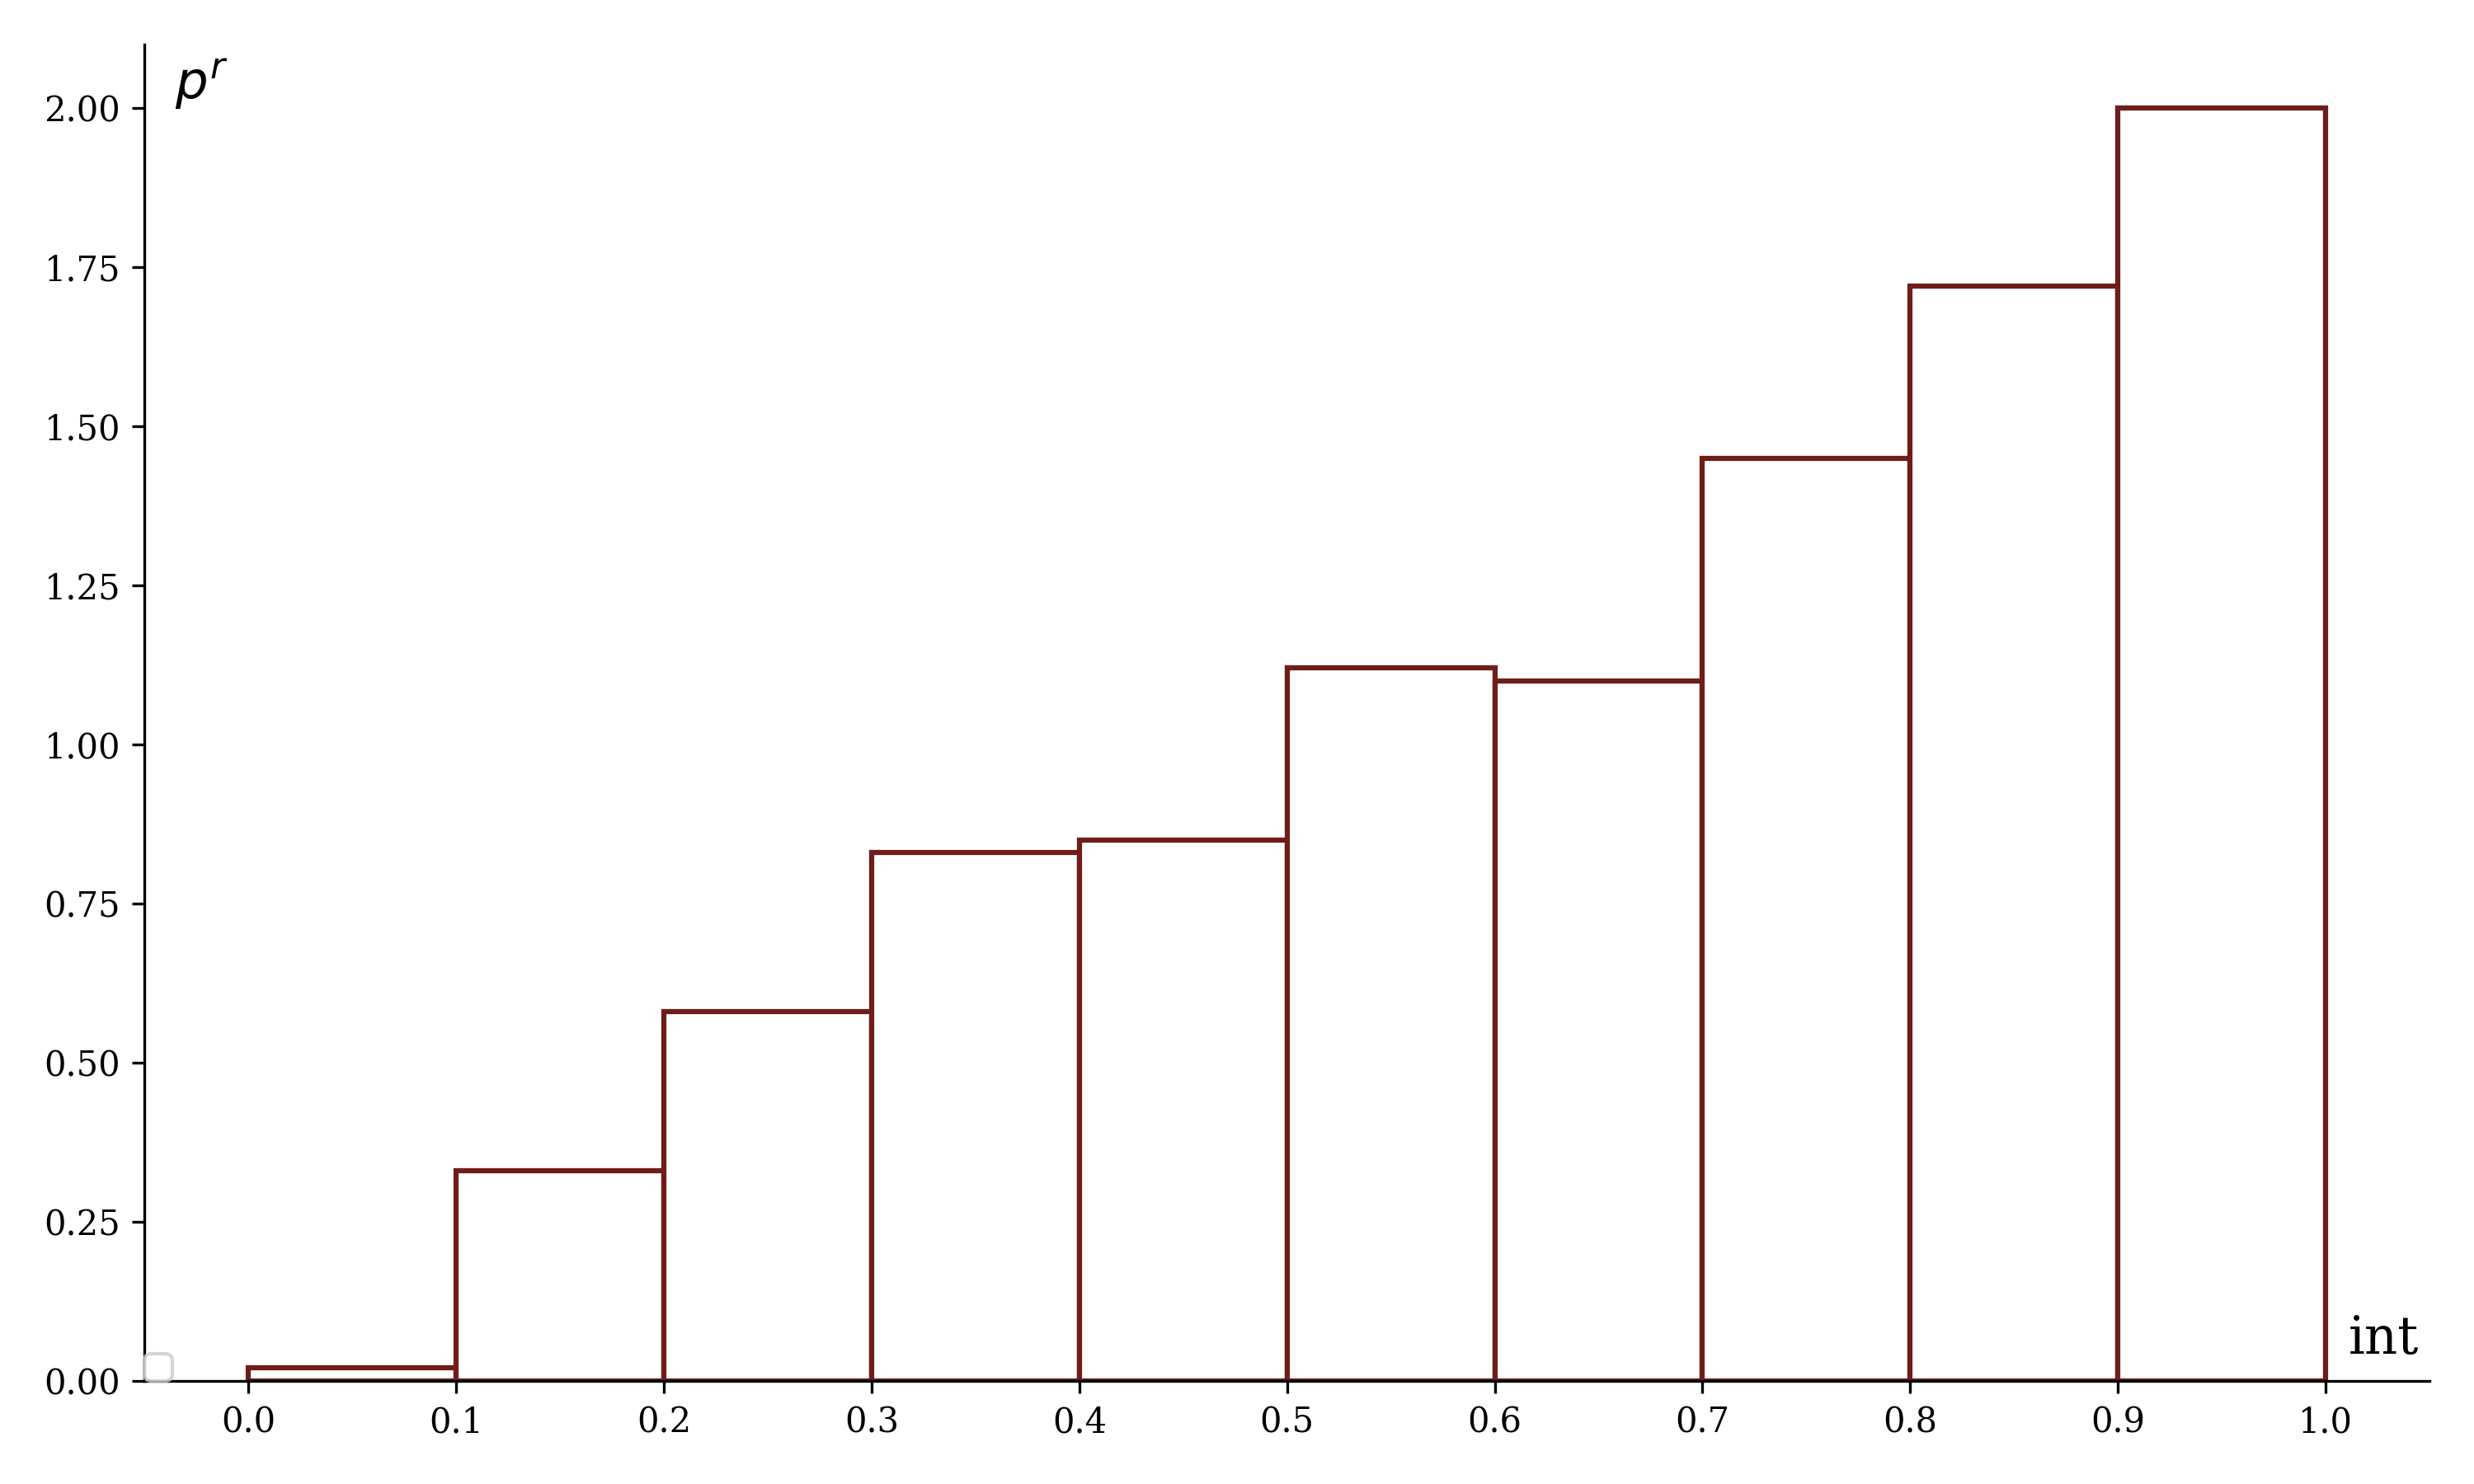
\includegraphics[width=\textwidth, height=\textheight, keepaspectratio]{sample24_hist}
\end{minipage}

\begin{minipage}[t]{0.25\textwidth}
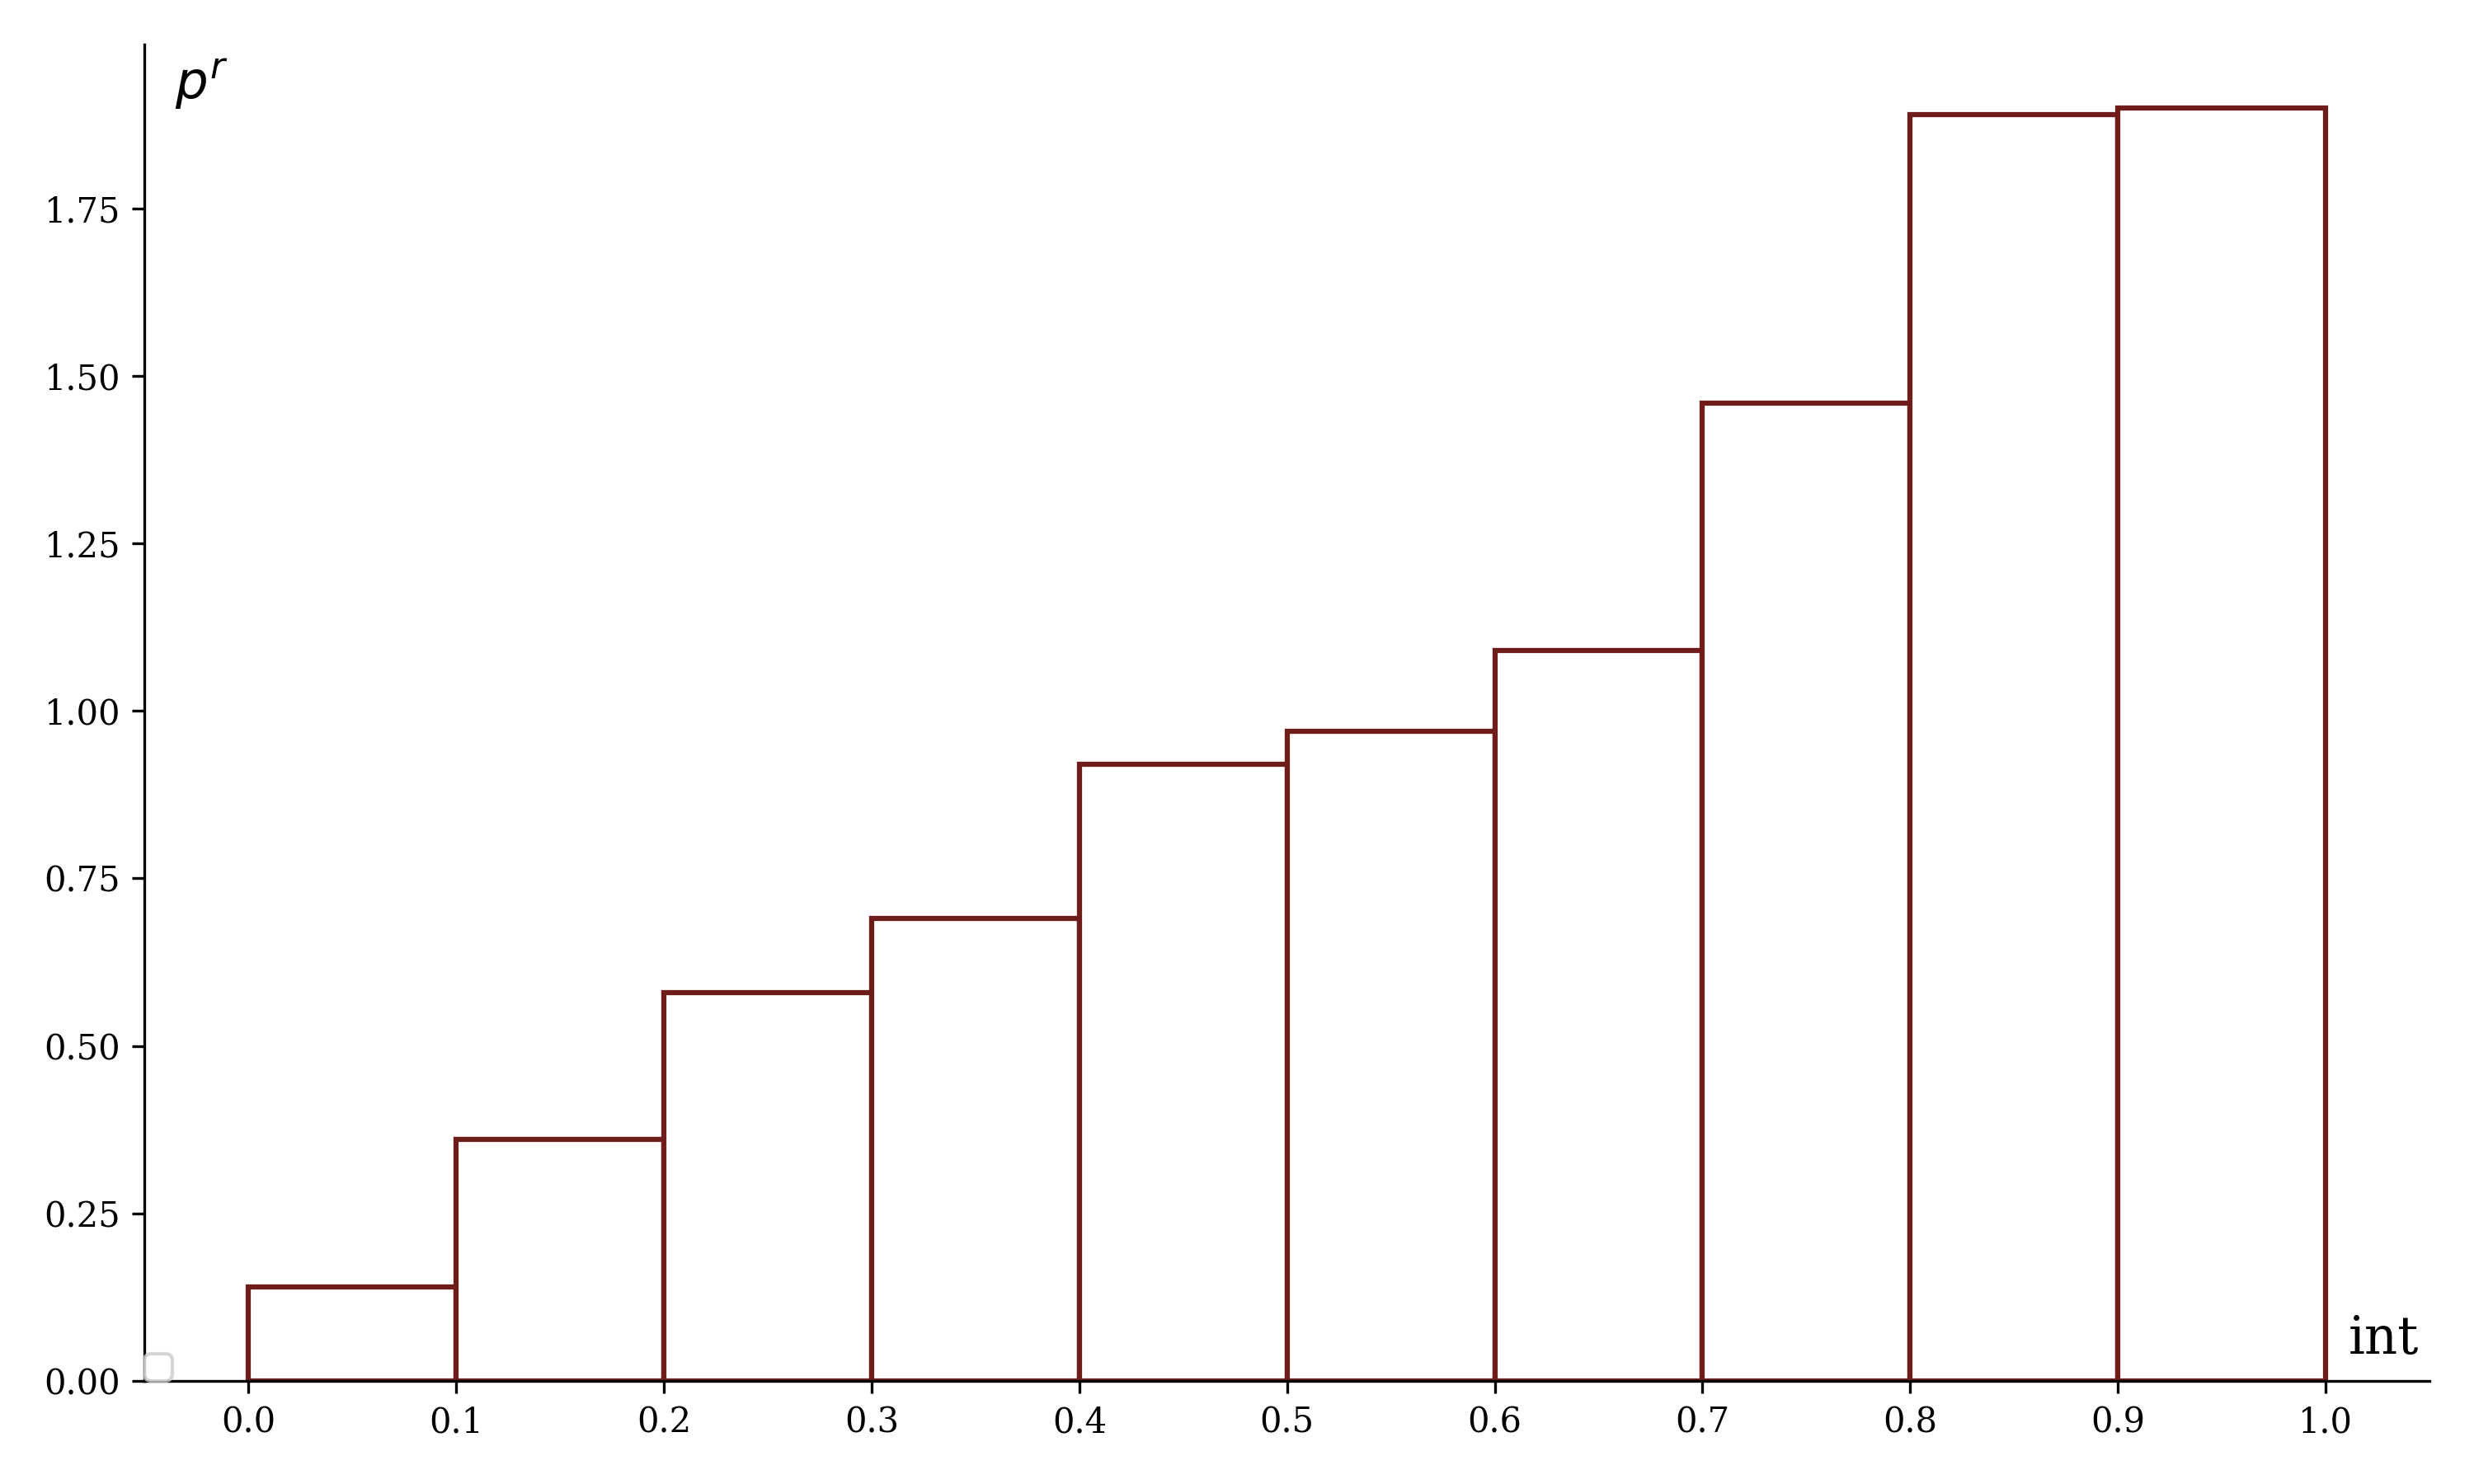
\includegraphics[width=\textwidth, height=\textheight, keepaspectratio]{sample25_hist}
\end{minipage}%
\begin{minipage}[t]{0.25\textwidth}
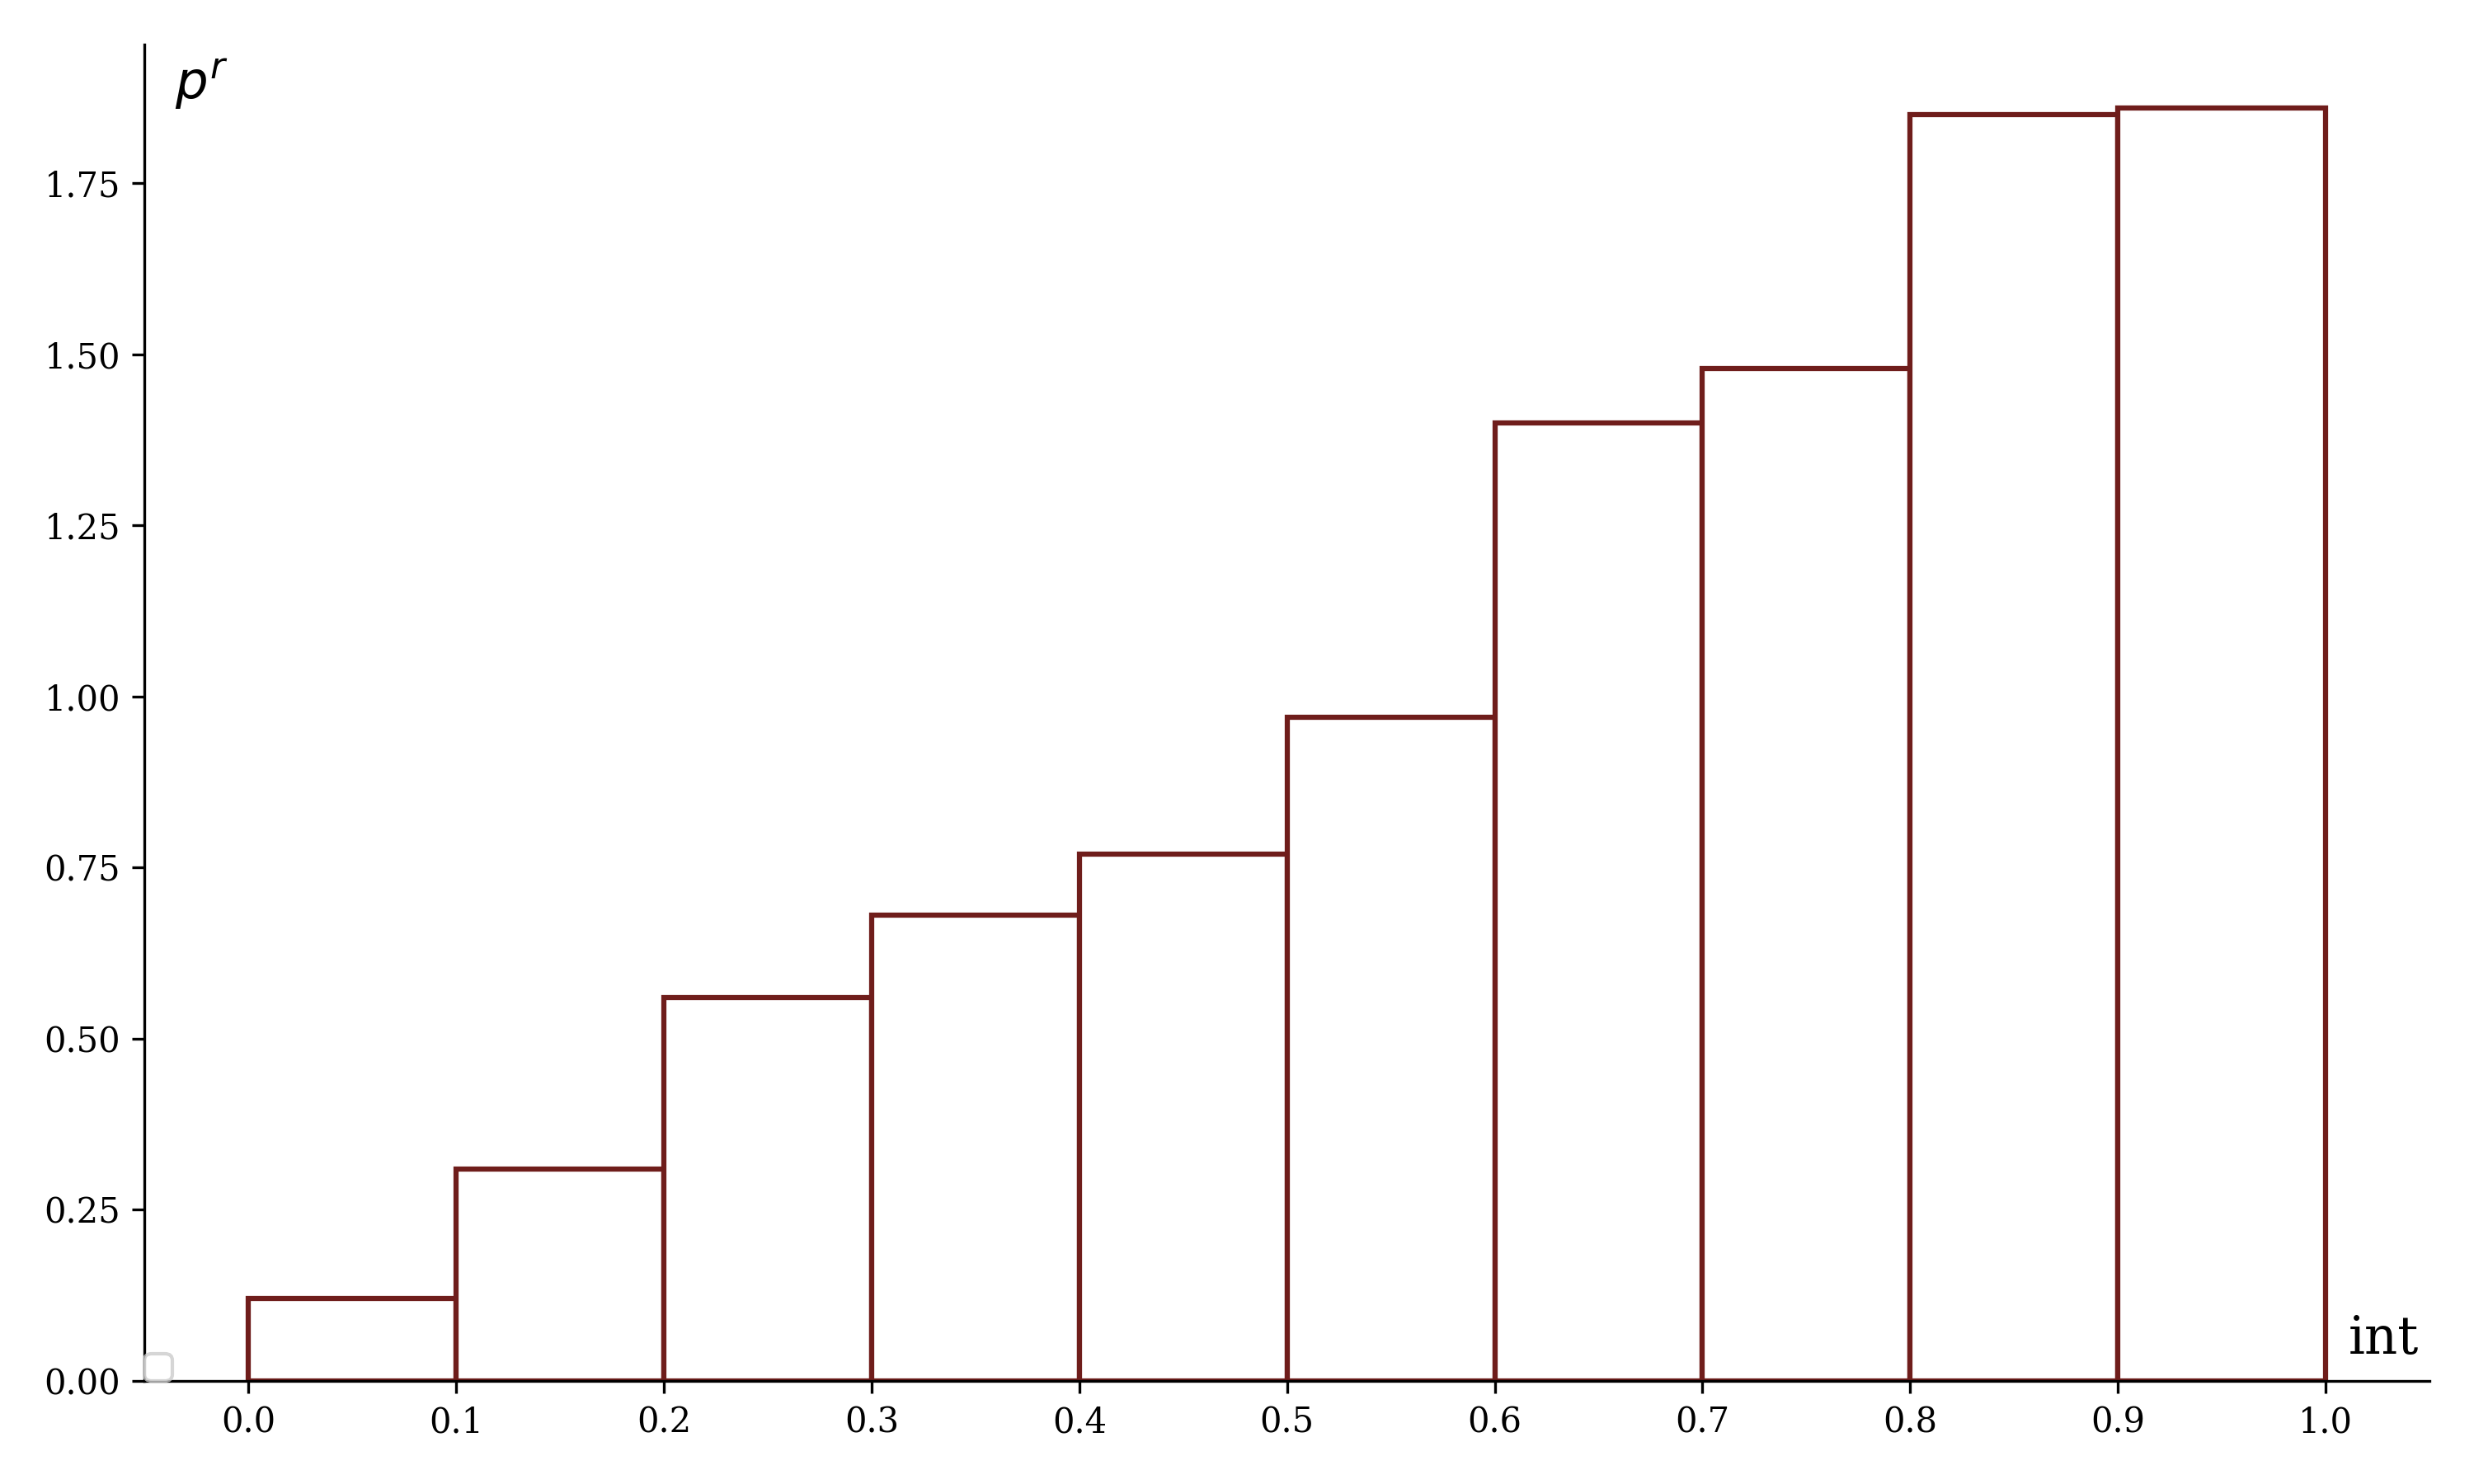
\includegraphics[width=\textwidth, height=\textheight, keepaspectratio]{sample26_hist}
\end{minipage}%
\begin{minipage}[t]{0.25\textwidth}
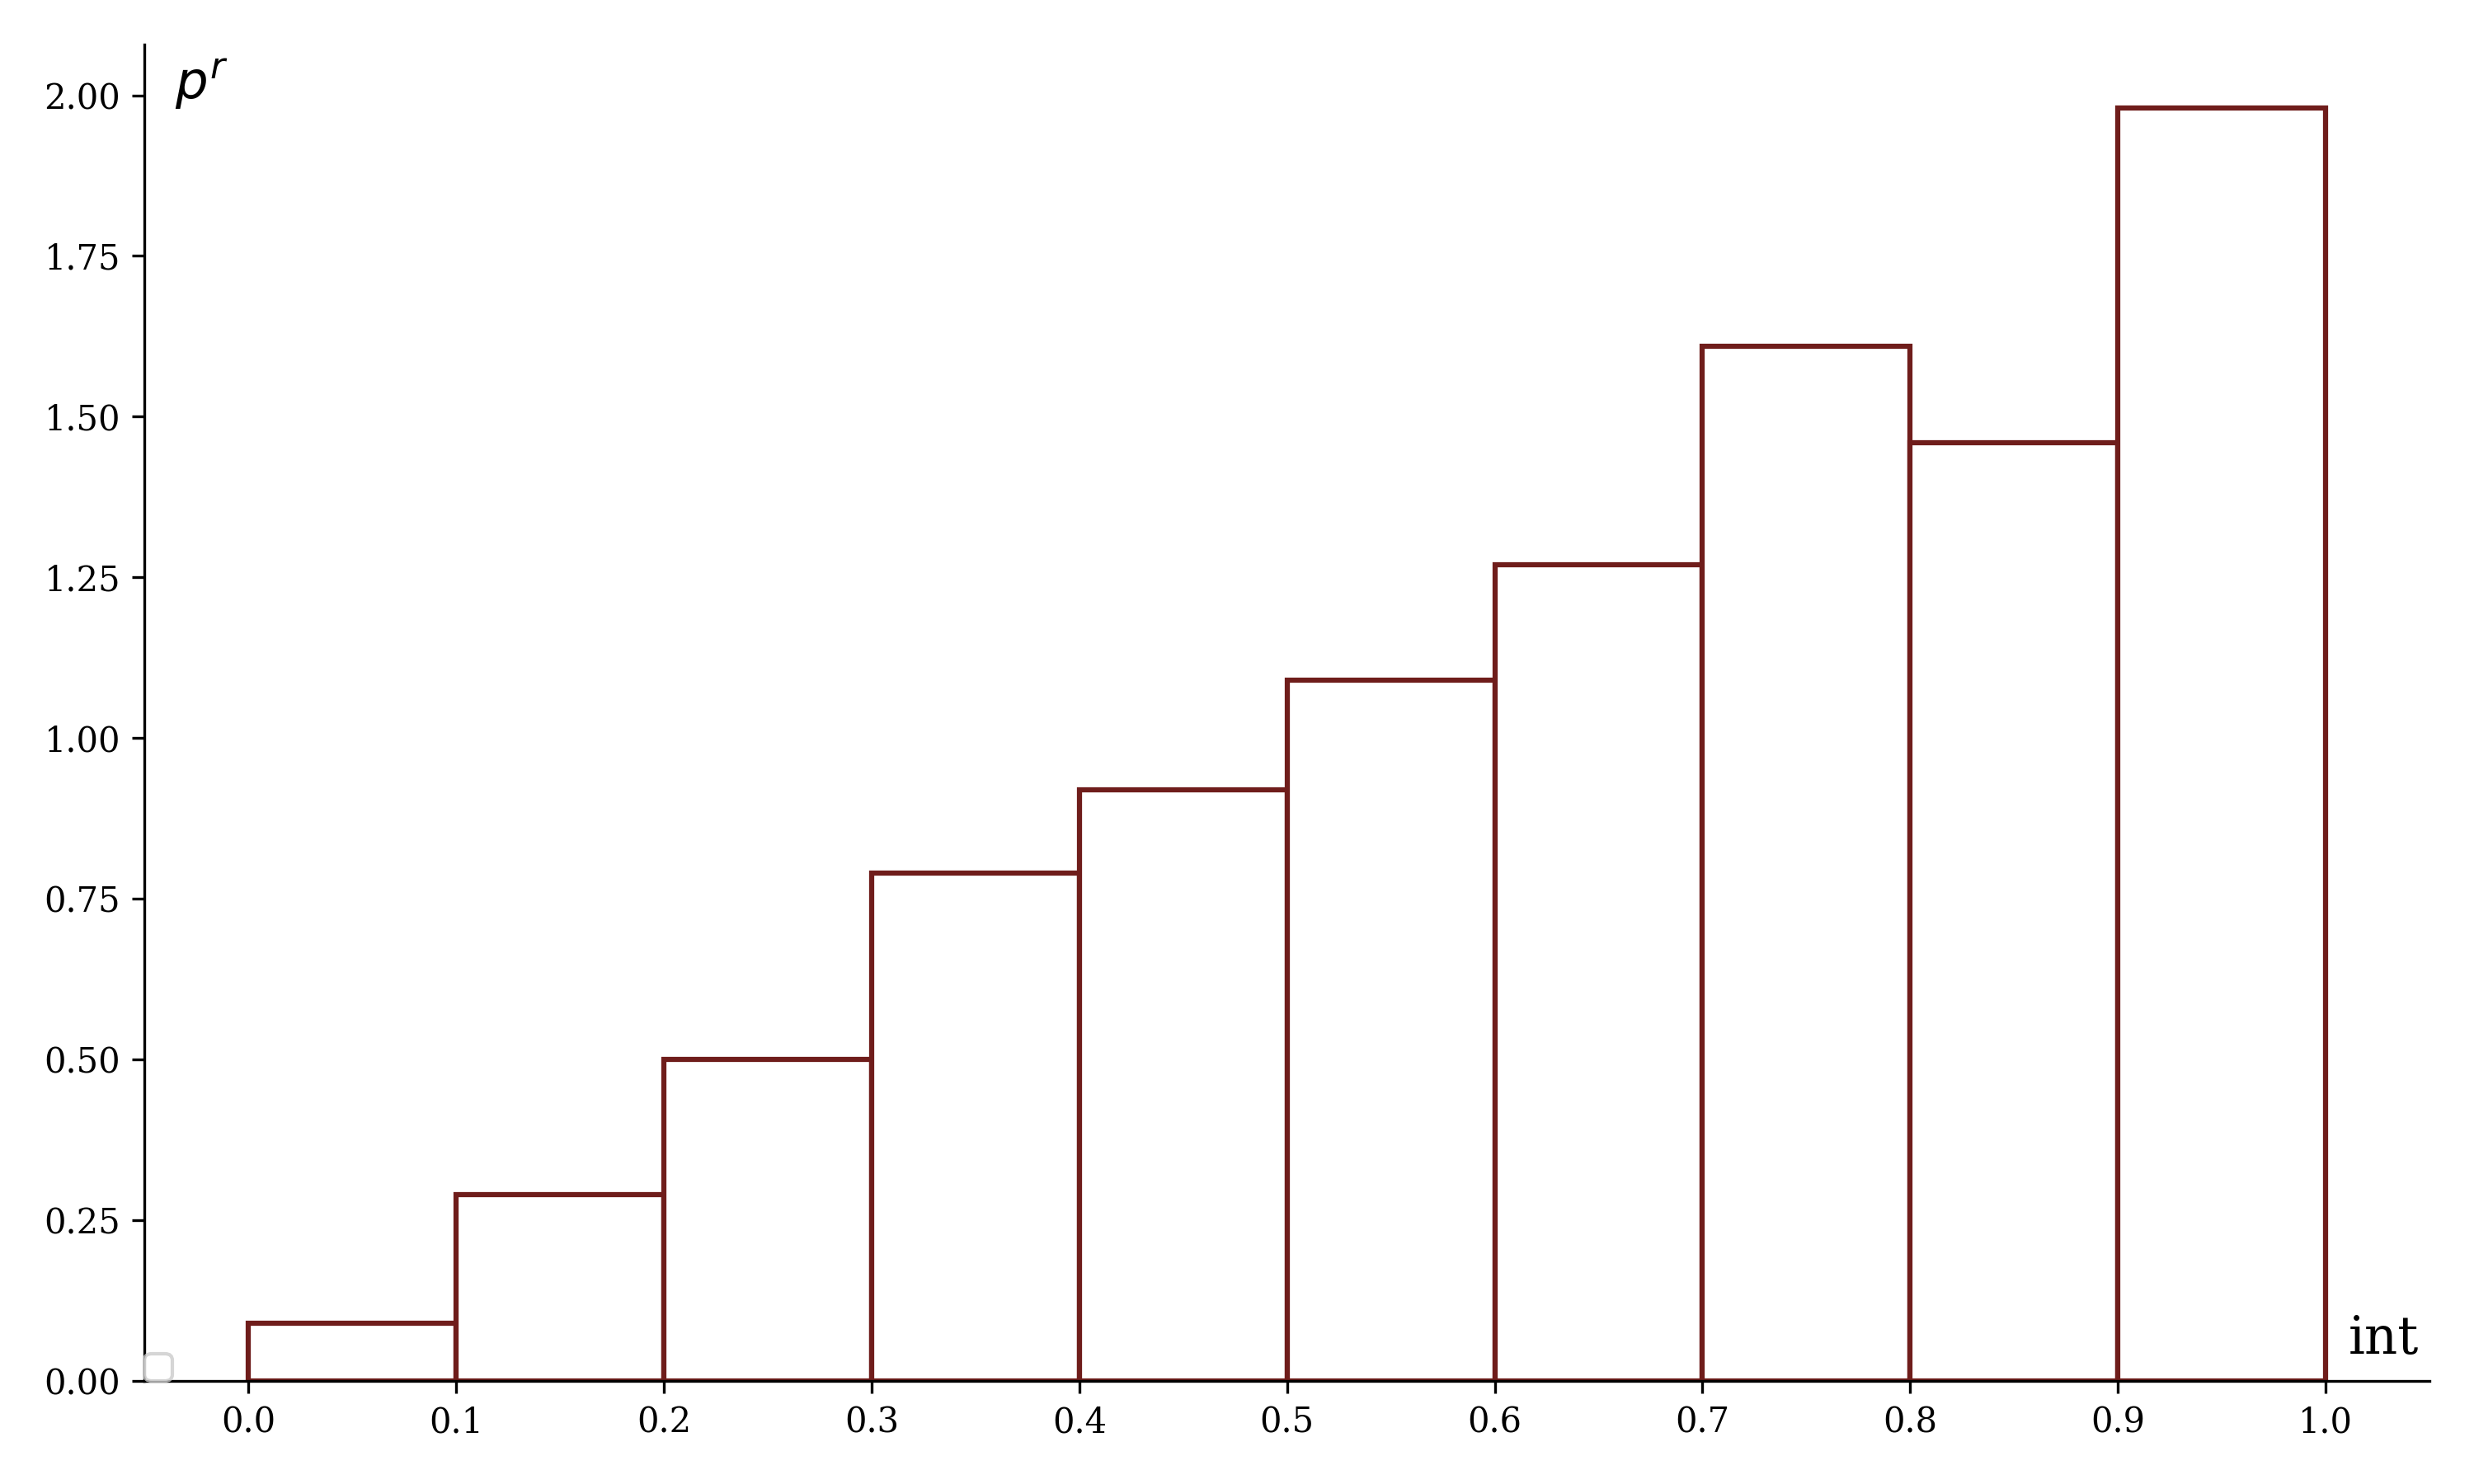
\includegraphics[width=\textwidth, height=\textheight, keepaspectratio]{sample27_hist}
\end{minipage}%
\begin{minipage}[t]{0.25\textwidth}
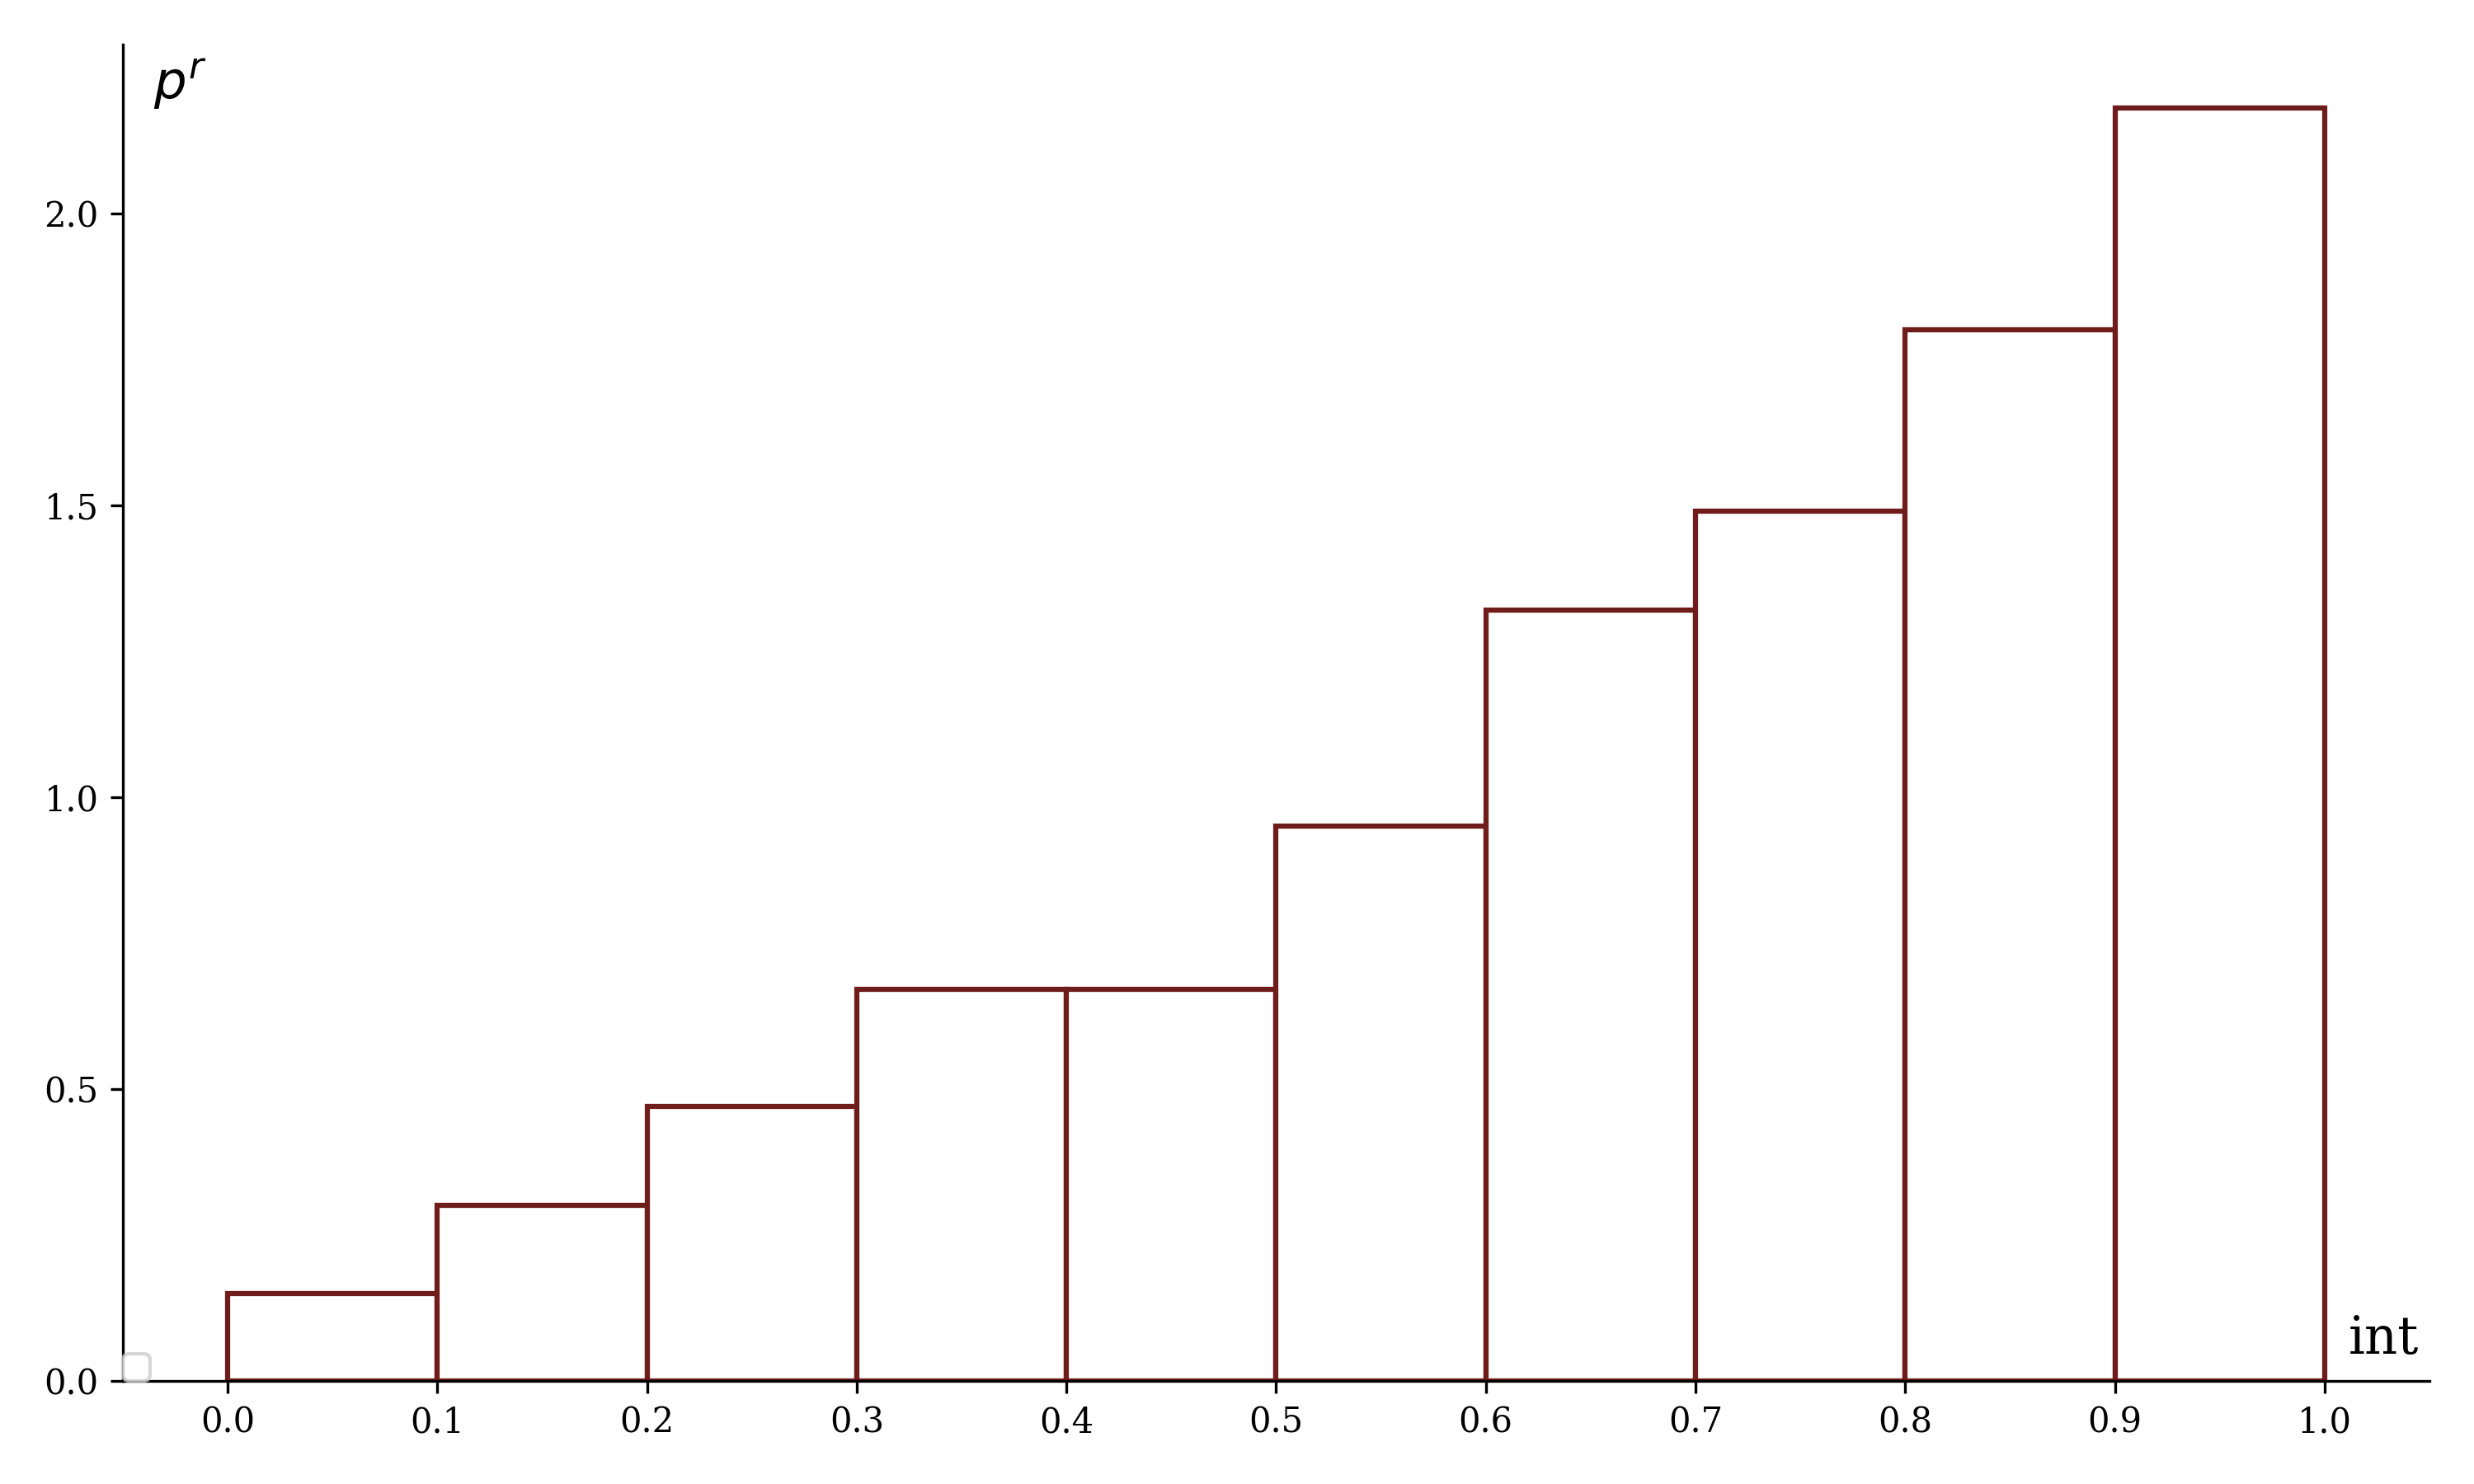
\includegraphics[width=\textwidth, height=\textheight, keepaspectratio]{sample28_hist}
\end{minipage}

\begin{minipage}[t]{0.25\textwidth}
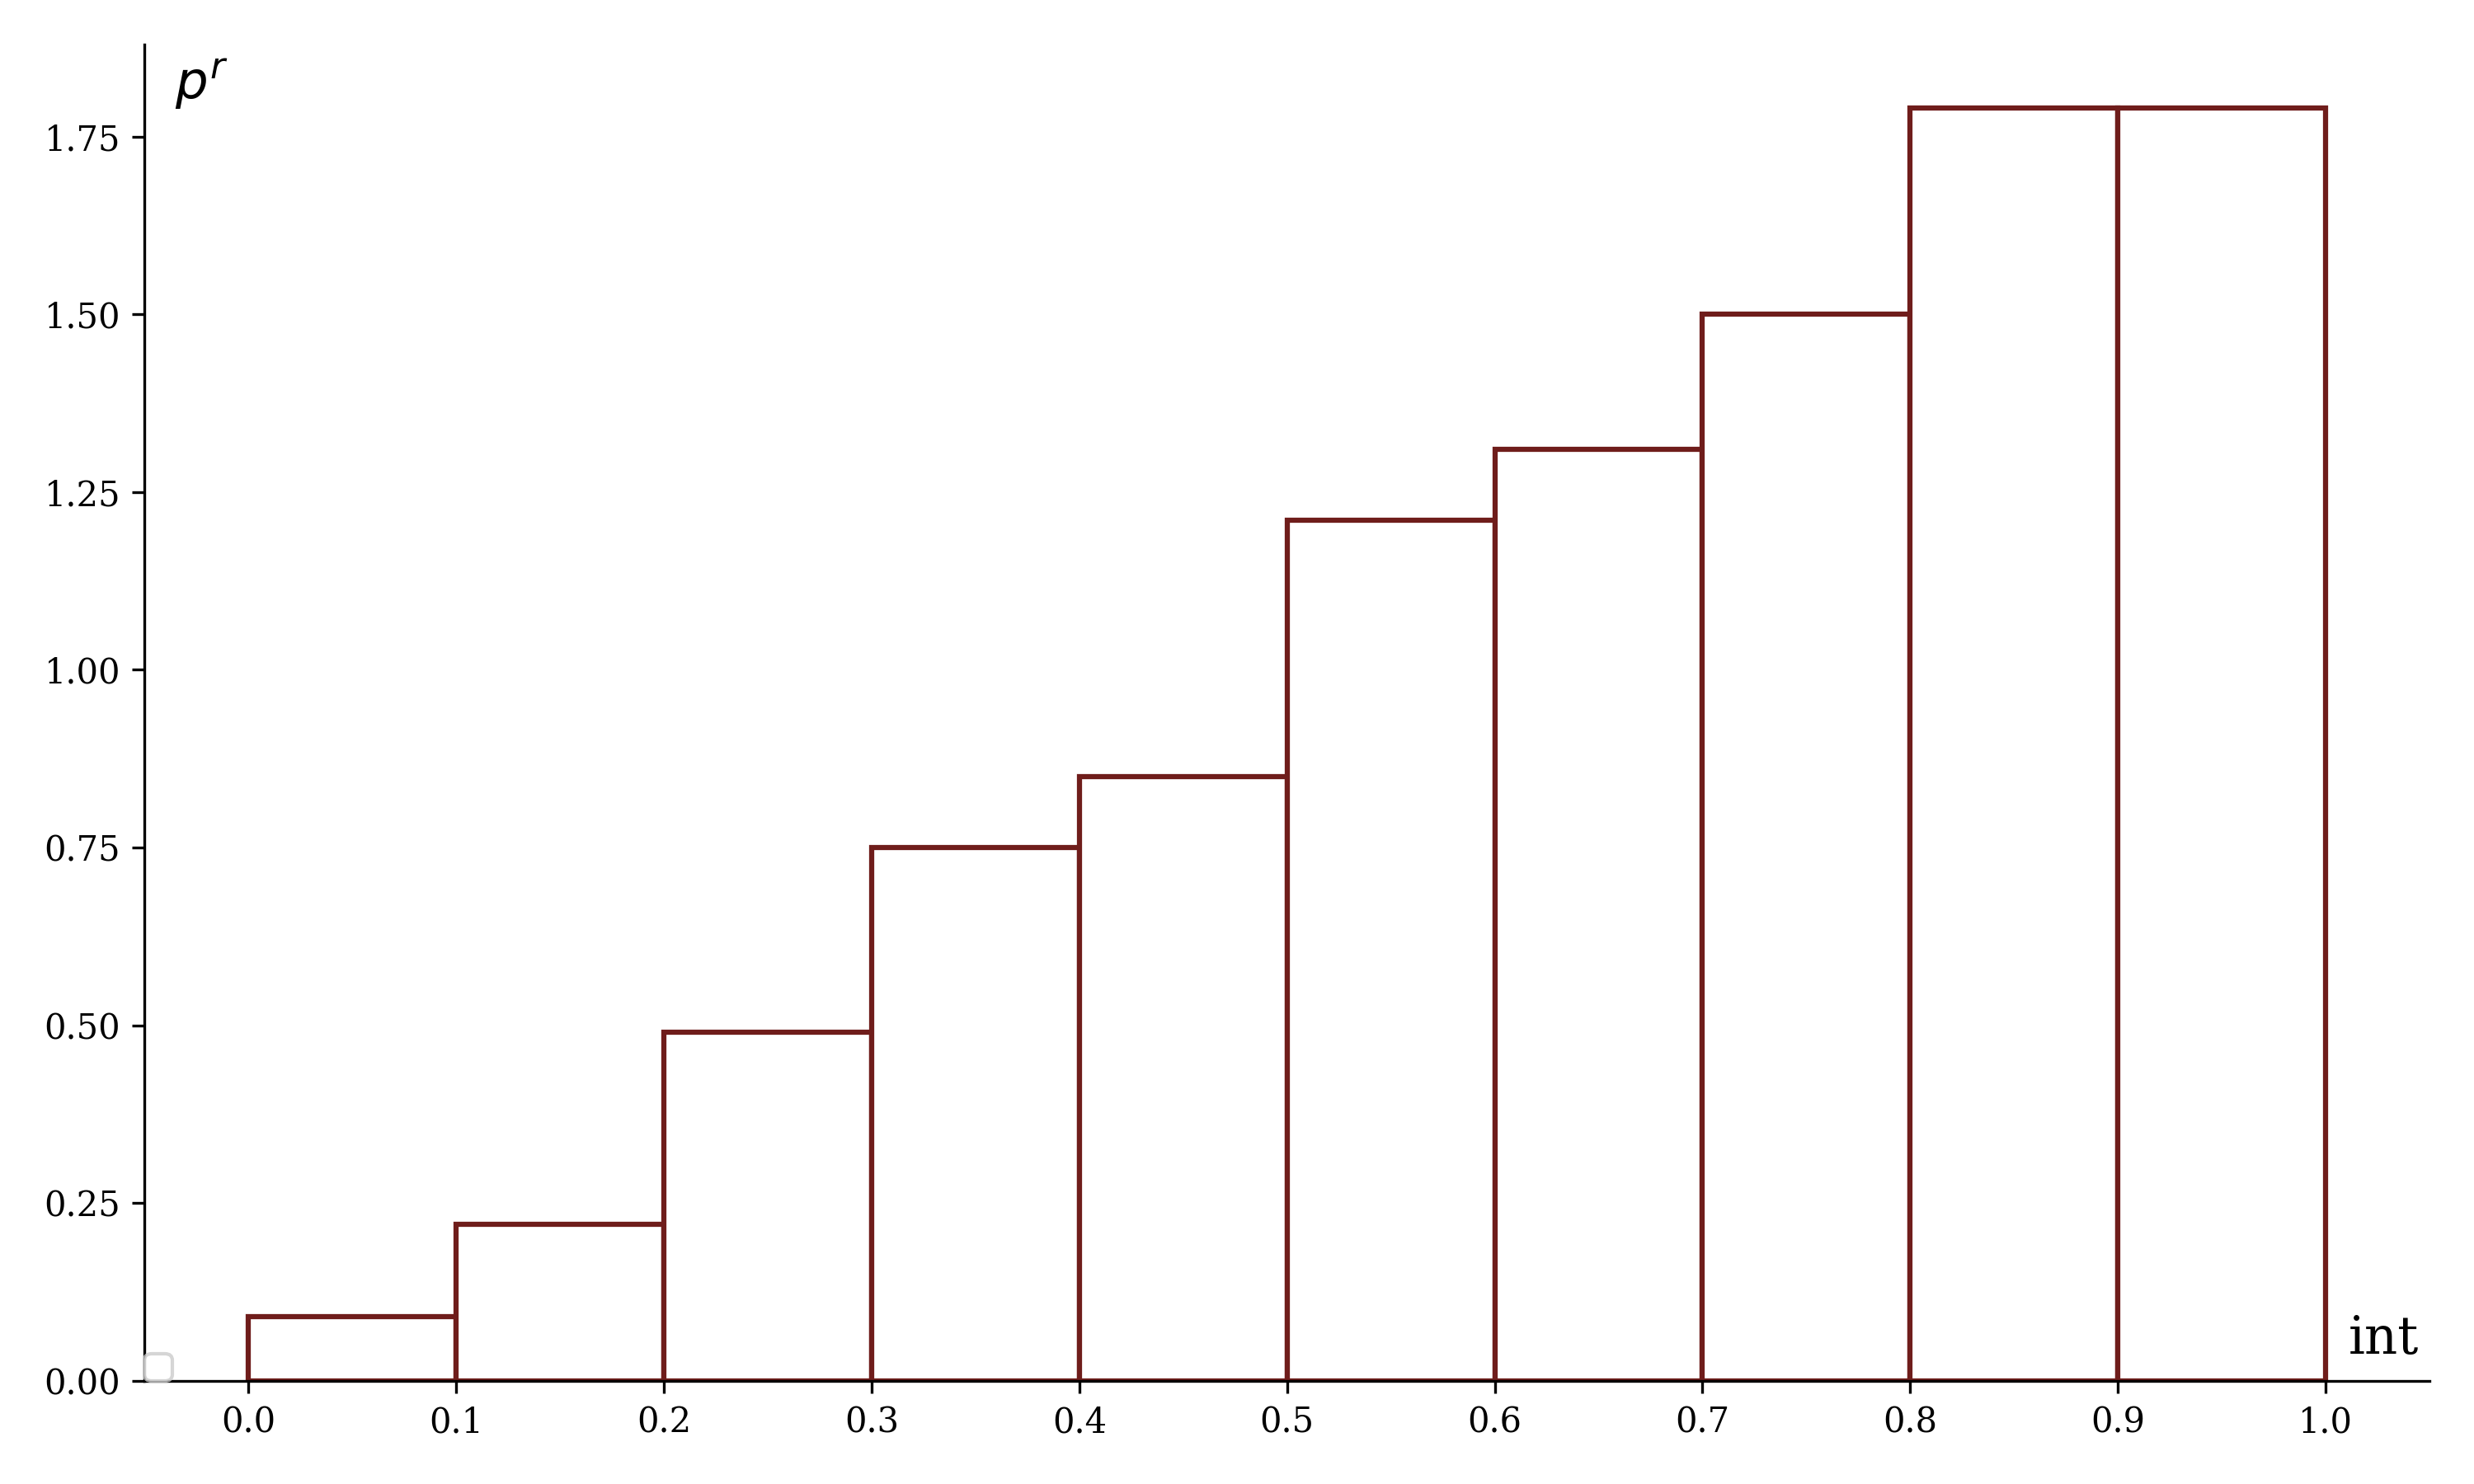
\includegraphics[width=\textwidth, height=\textheight, keepaspectratio]{sample29_hist}
\end{minipage}%
\begin{minipage}[t]{0.25\textwidth}
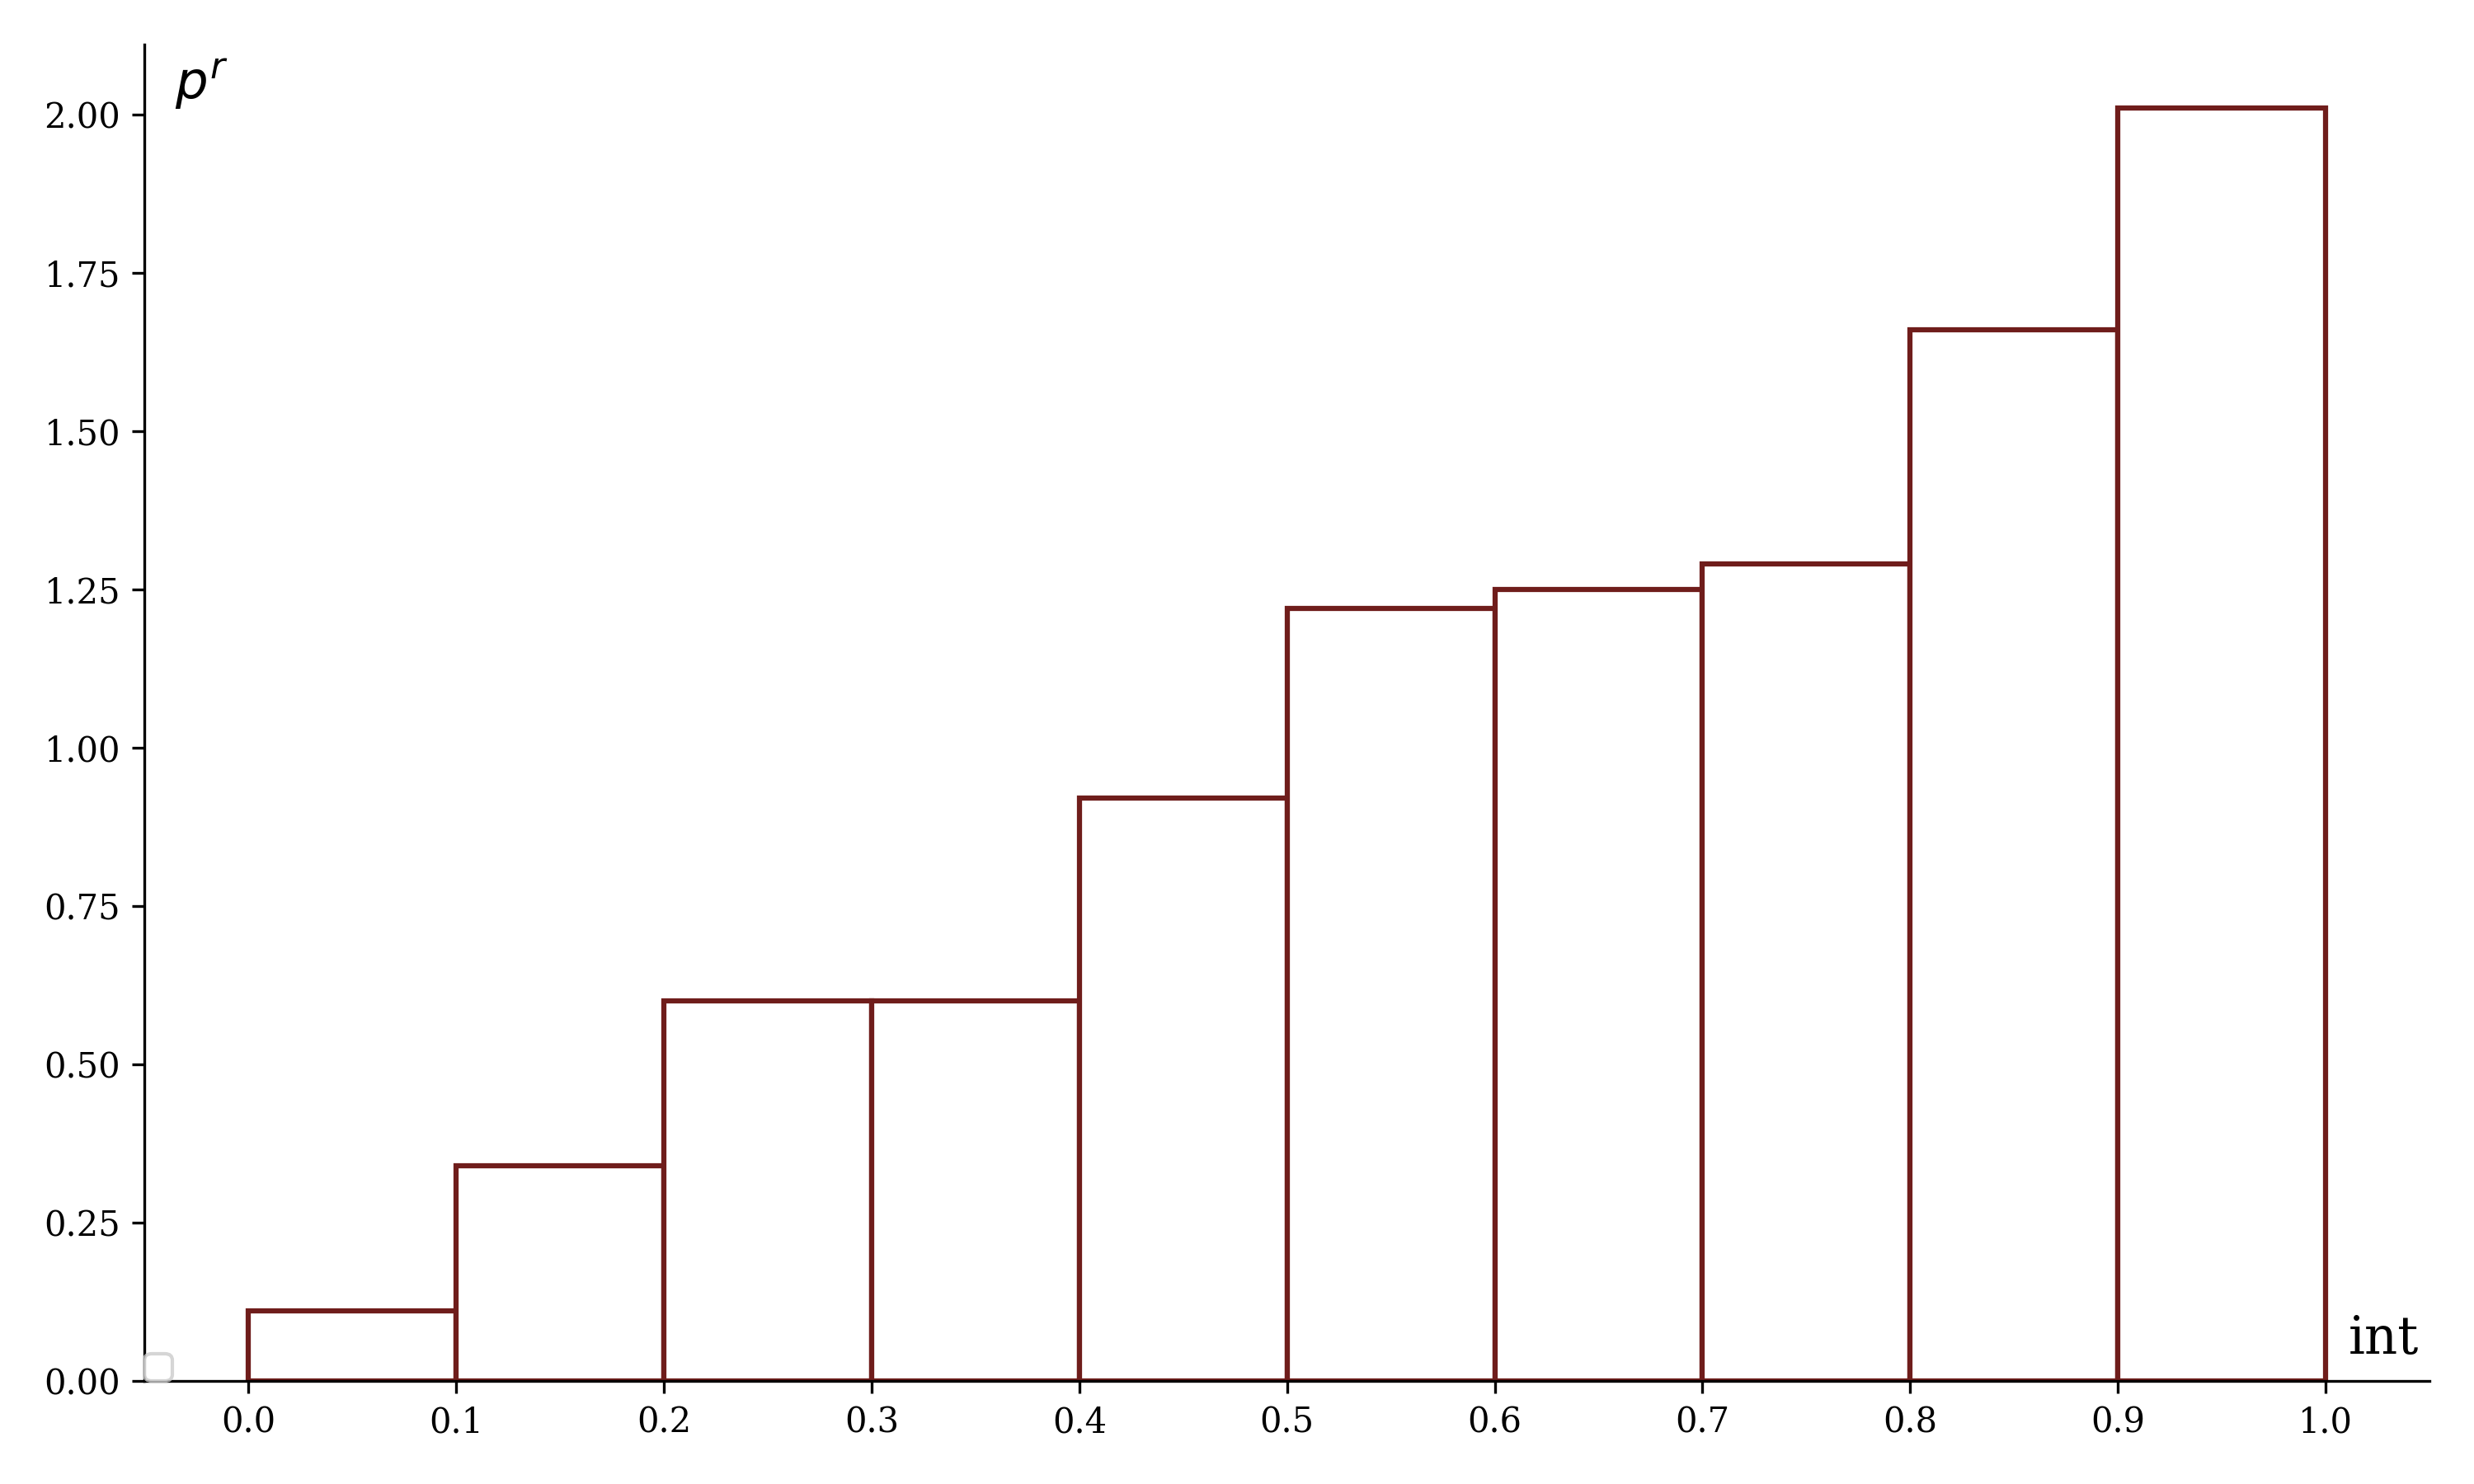
\includegraphics[width=\textwidth, height=\textheight, keepaspectratio]{sample30_hist}
\end{minipage}%
\begin{minipage}[t]{0.25\textwidth}
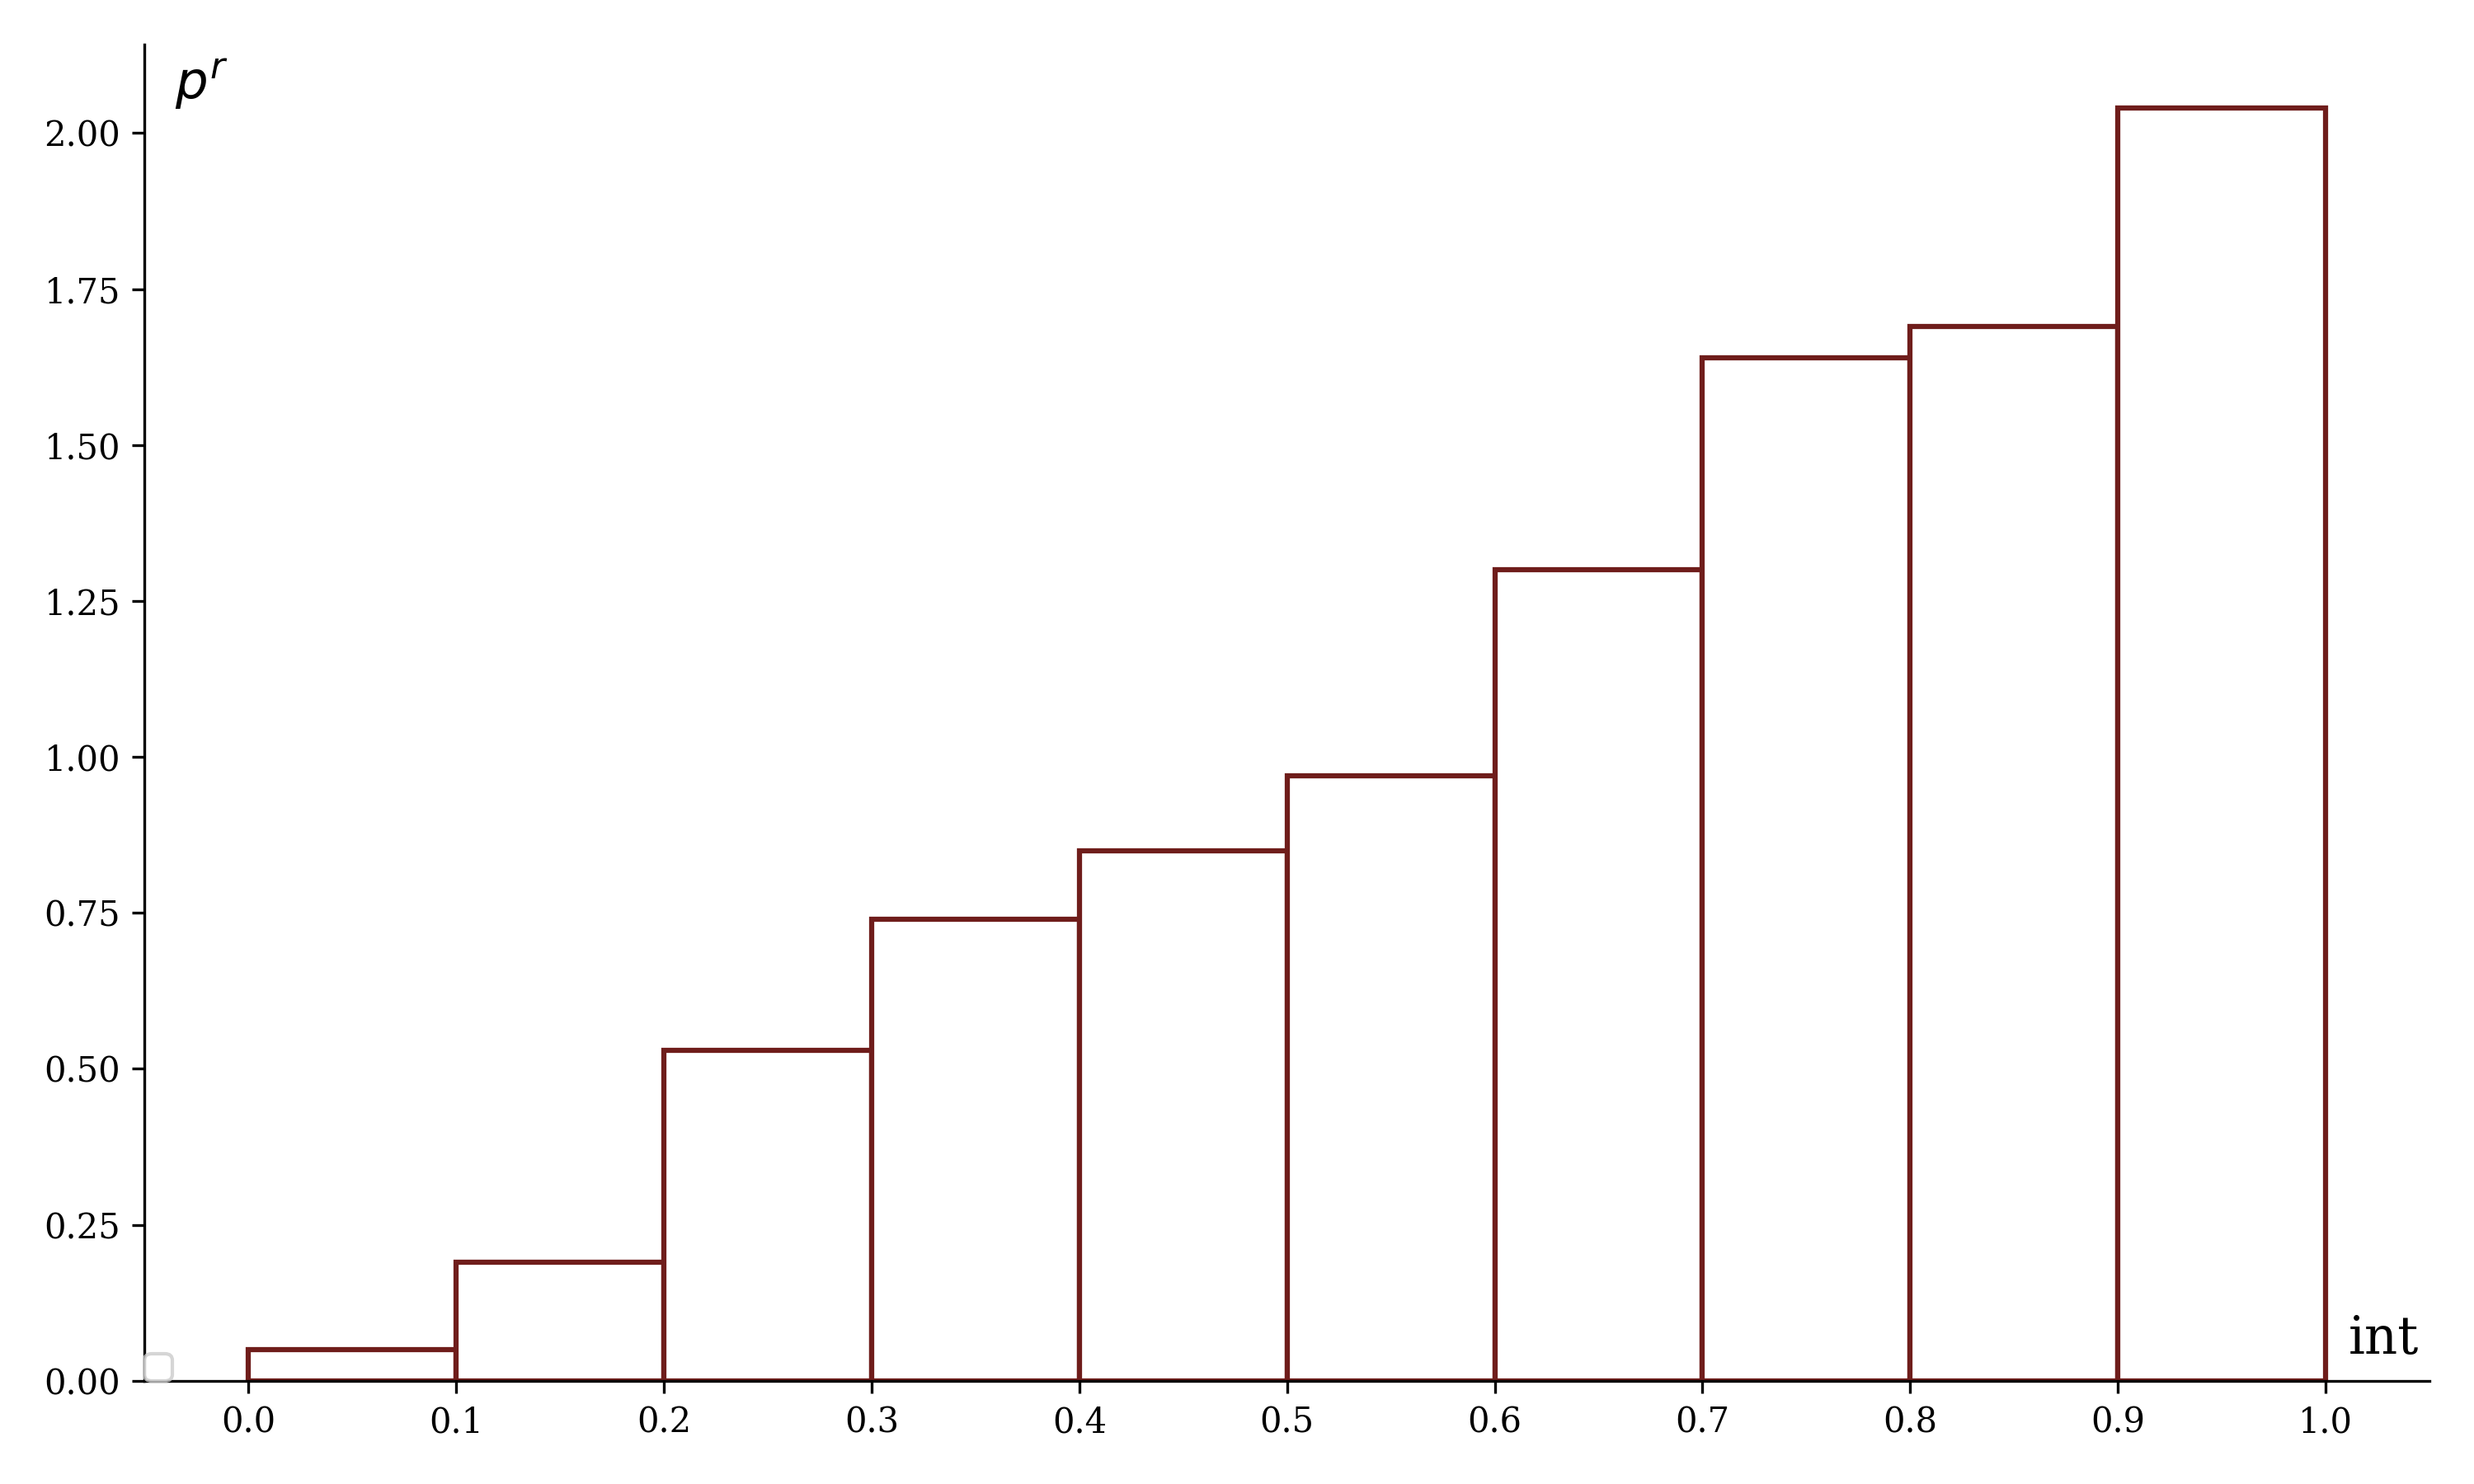
\includegraphics[width=\textwidth, height=\textheight, keepaspectratio]{sample31_hist}
\end{minipage}%
\begin{minipage}[t]{0.25\textwidth}
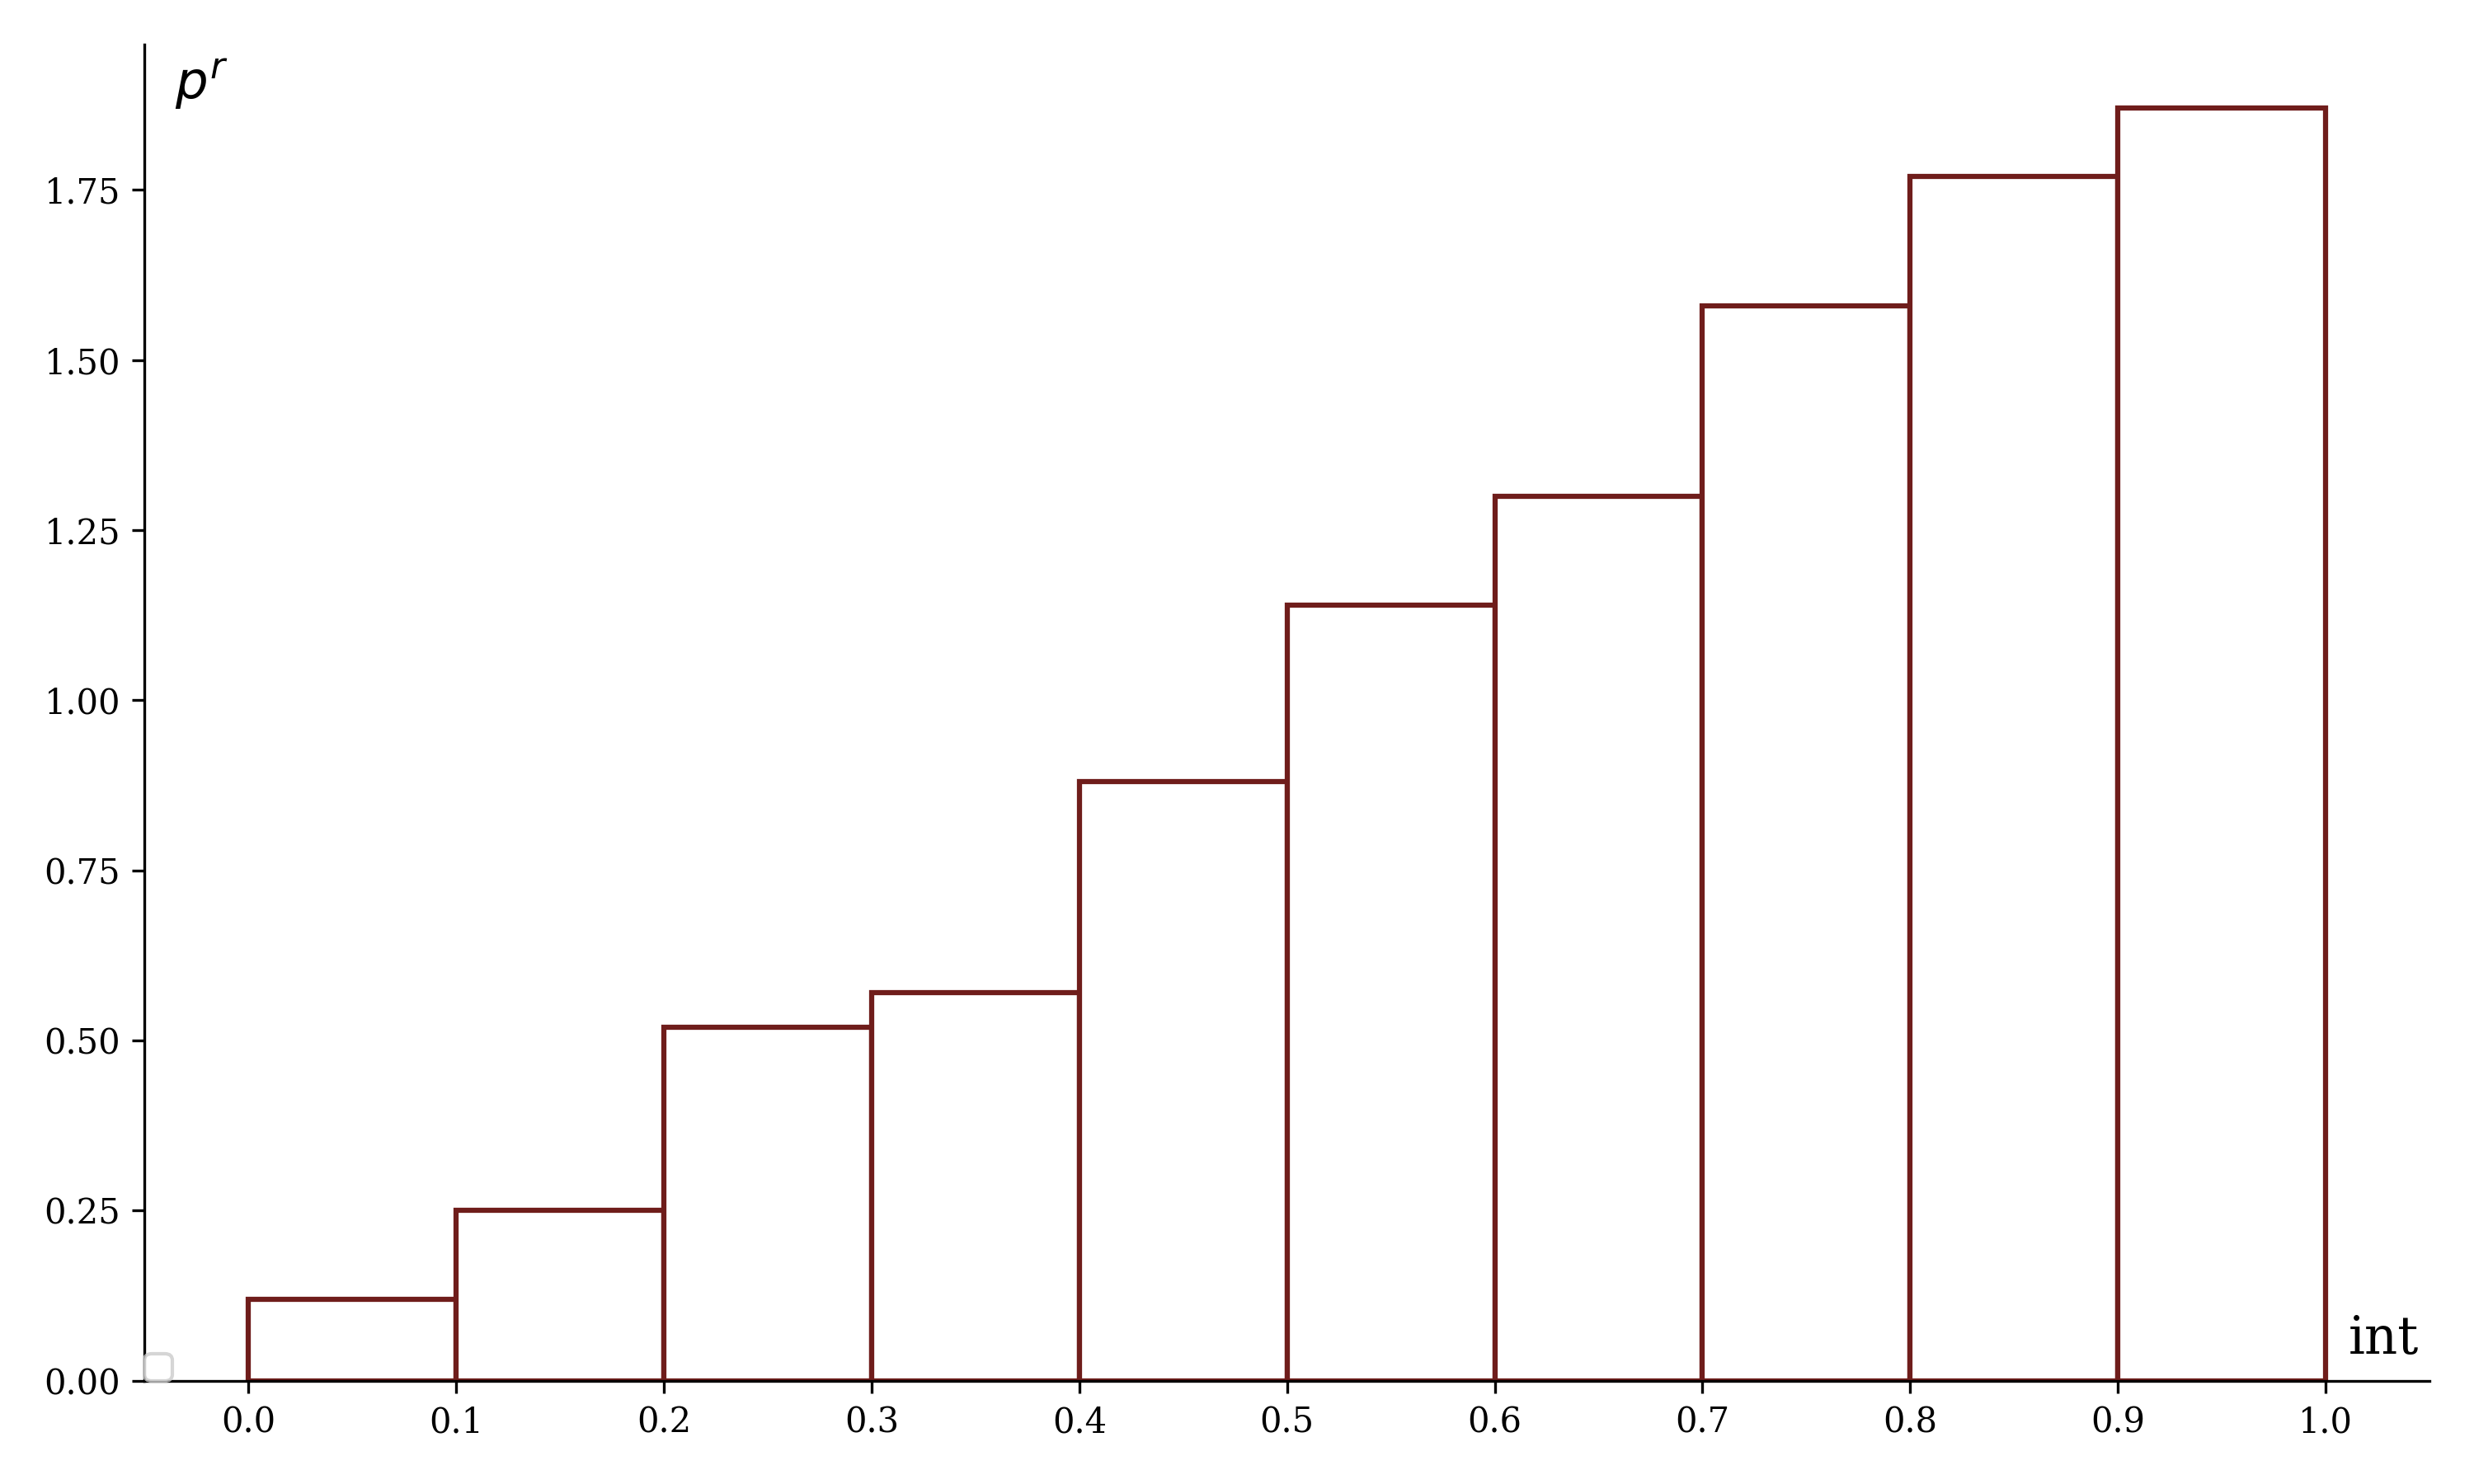
\includegraphics[width=\textwidth, height=\textheight, keepaspectratio]{sample32_hist}
\end{minipage}

\begin{minipage}[t]{0.25\textwidth}
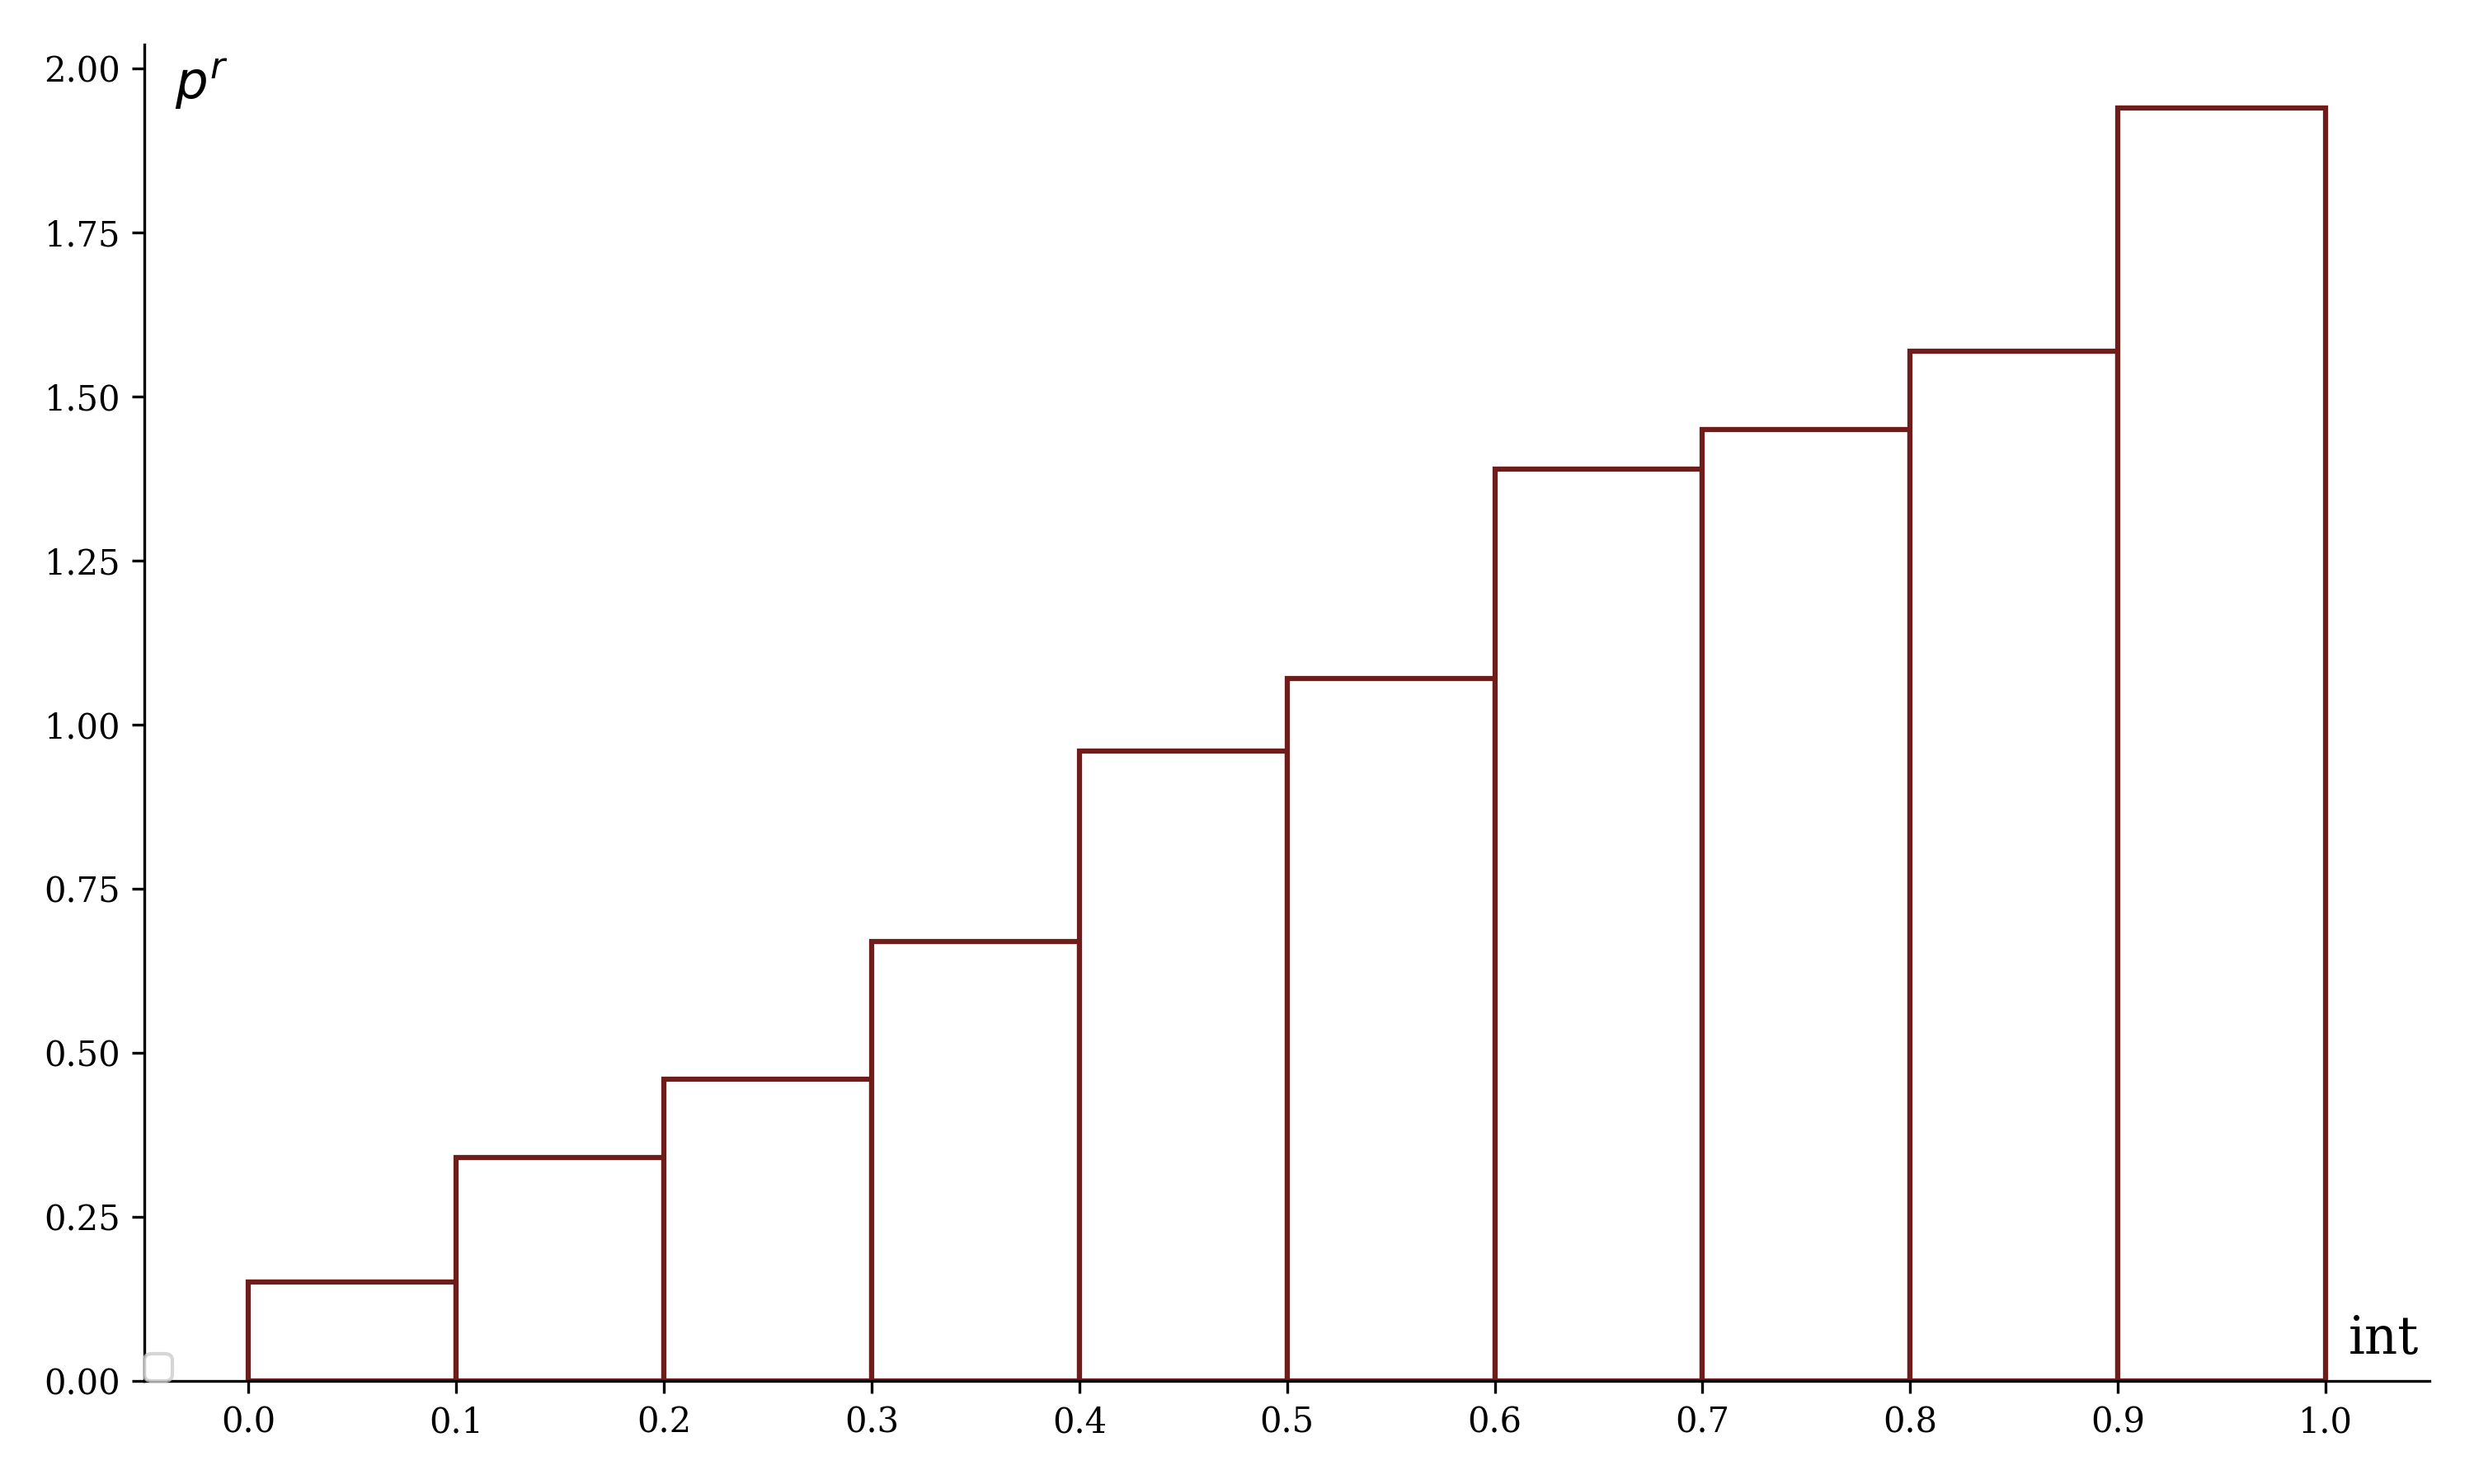
\includegraphics[width=\textwidth, height=\textheight, keepaspectratio]{sample33_hist}
\end{minipage}%
\begin{minipage}[t]{0.25\textwidth}
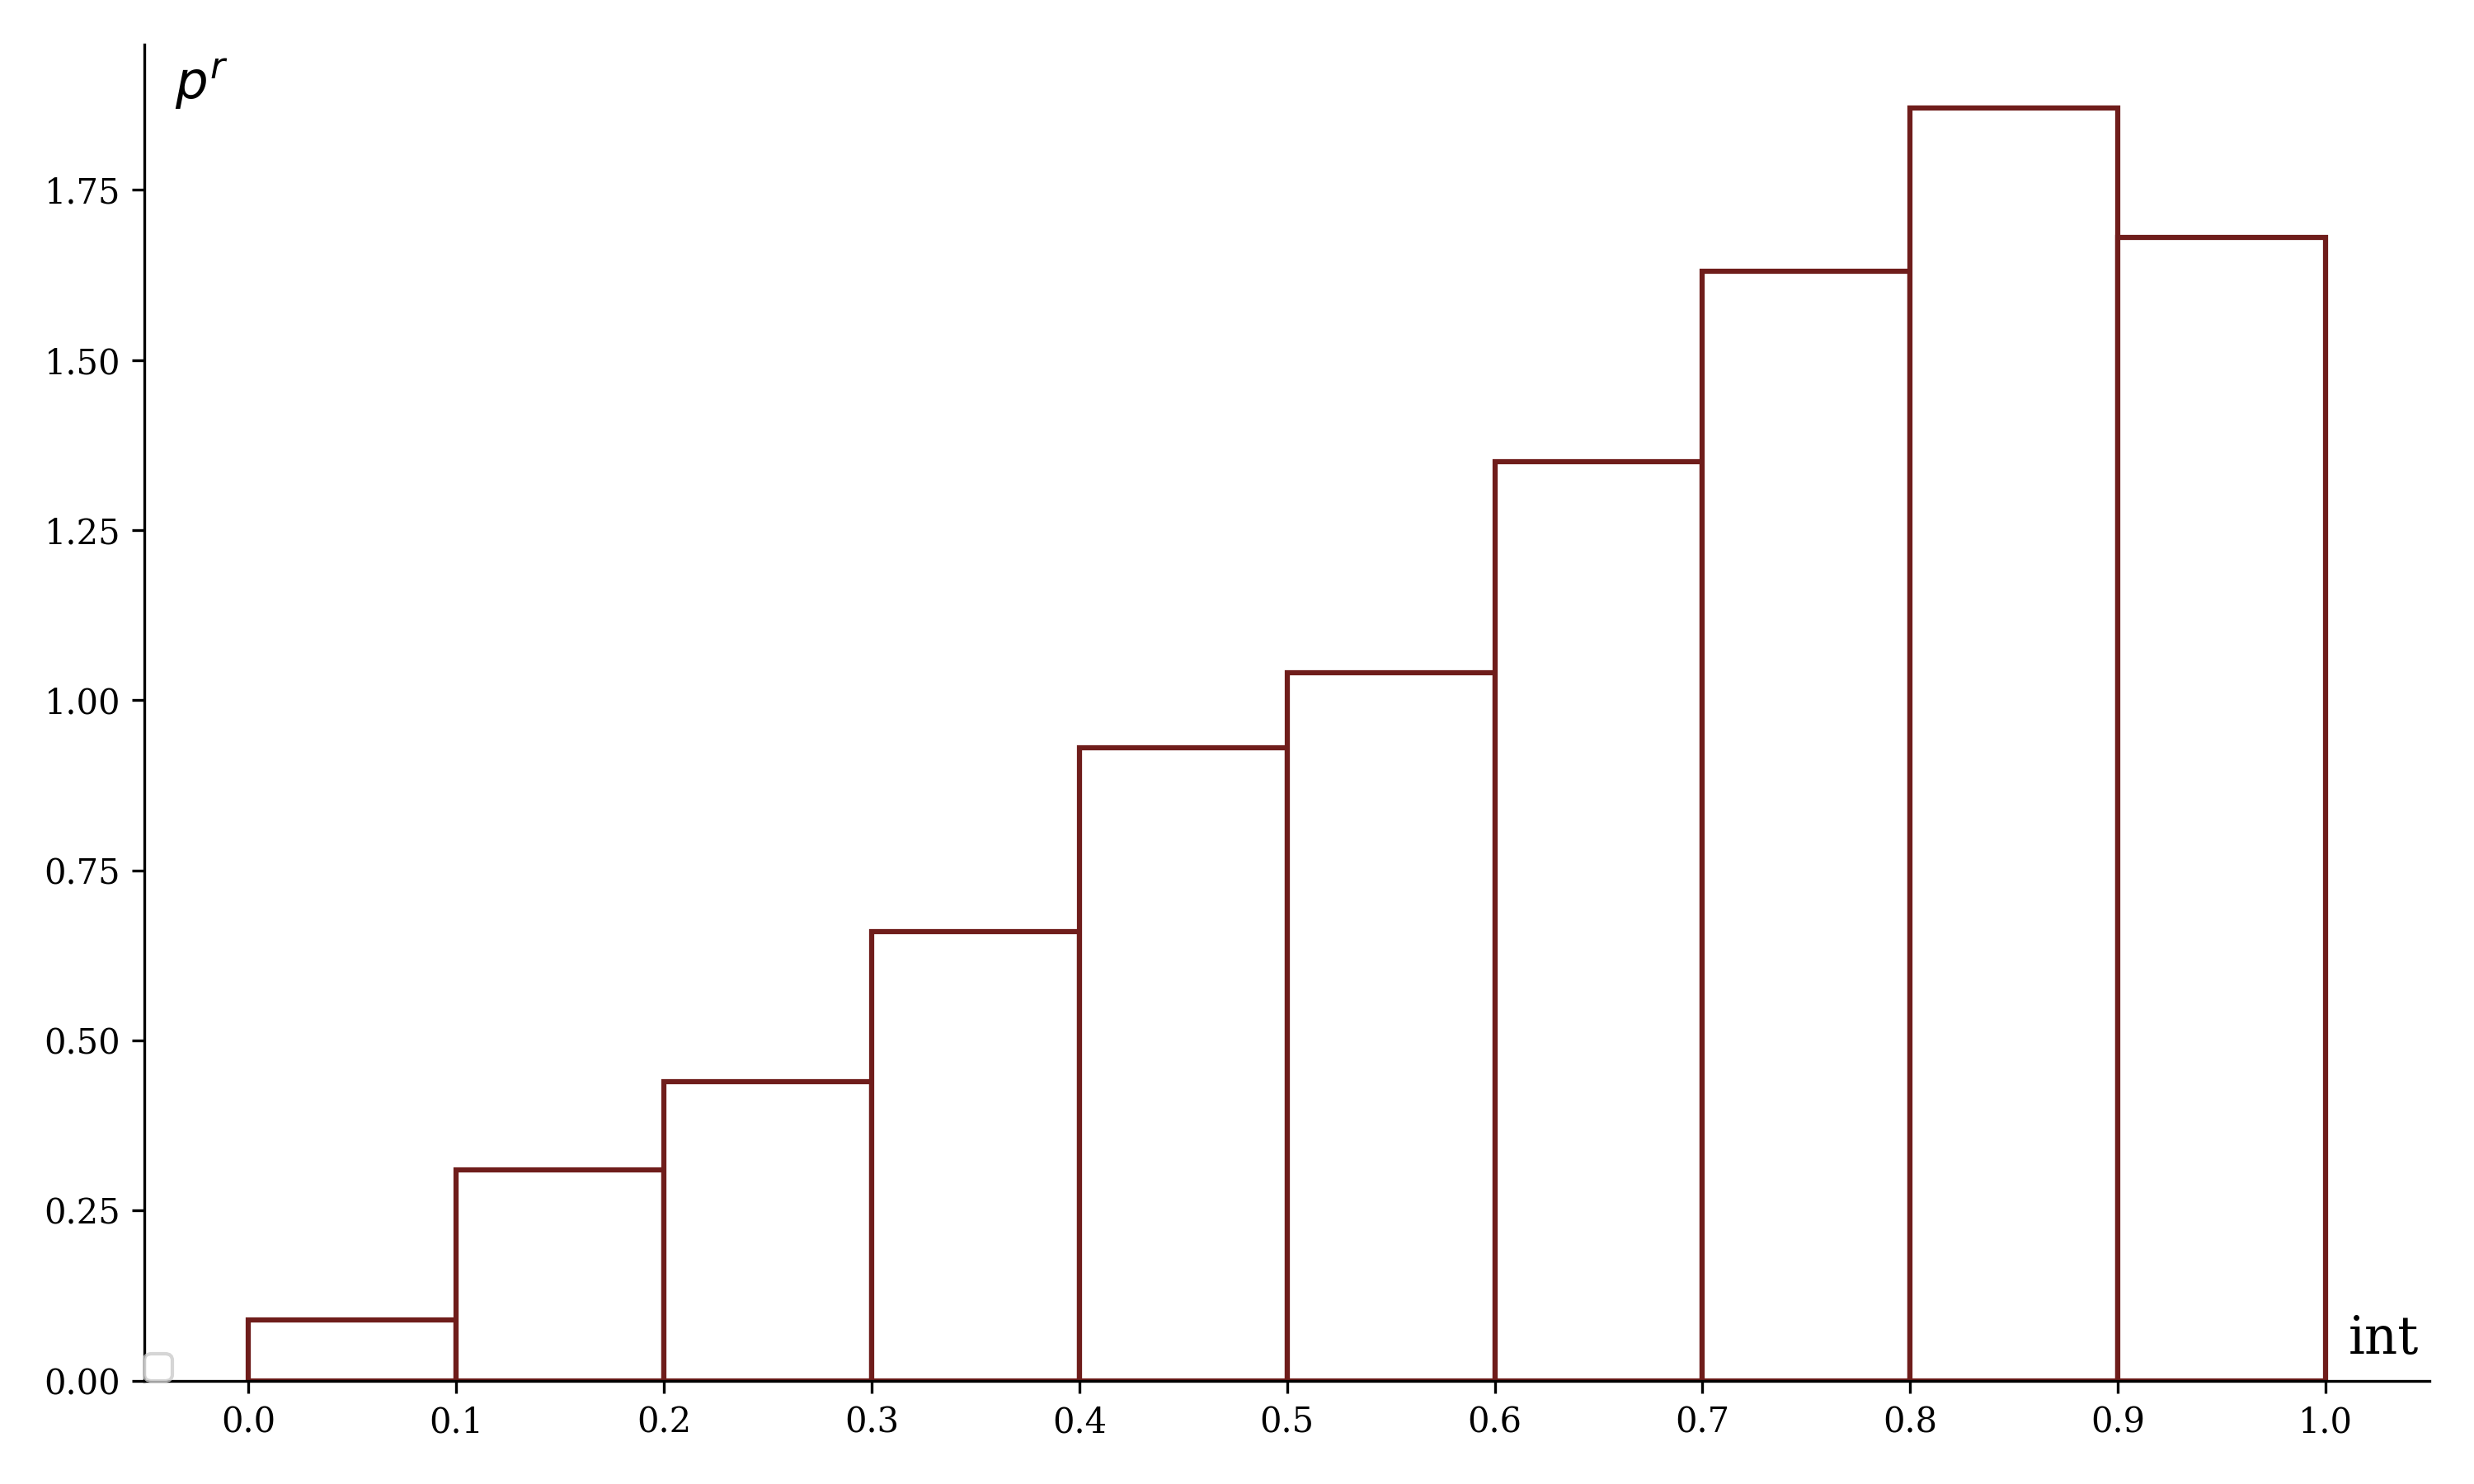
\includegraphics[width=\textwidth, height=\textheight, keepaspectratio]{sample34_hist}
\end{minipage}%
\begin{minipage}[t]{0.25\textwidth}
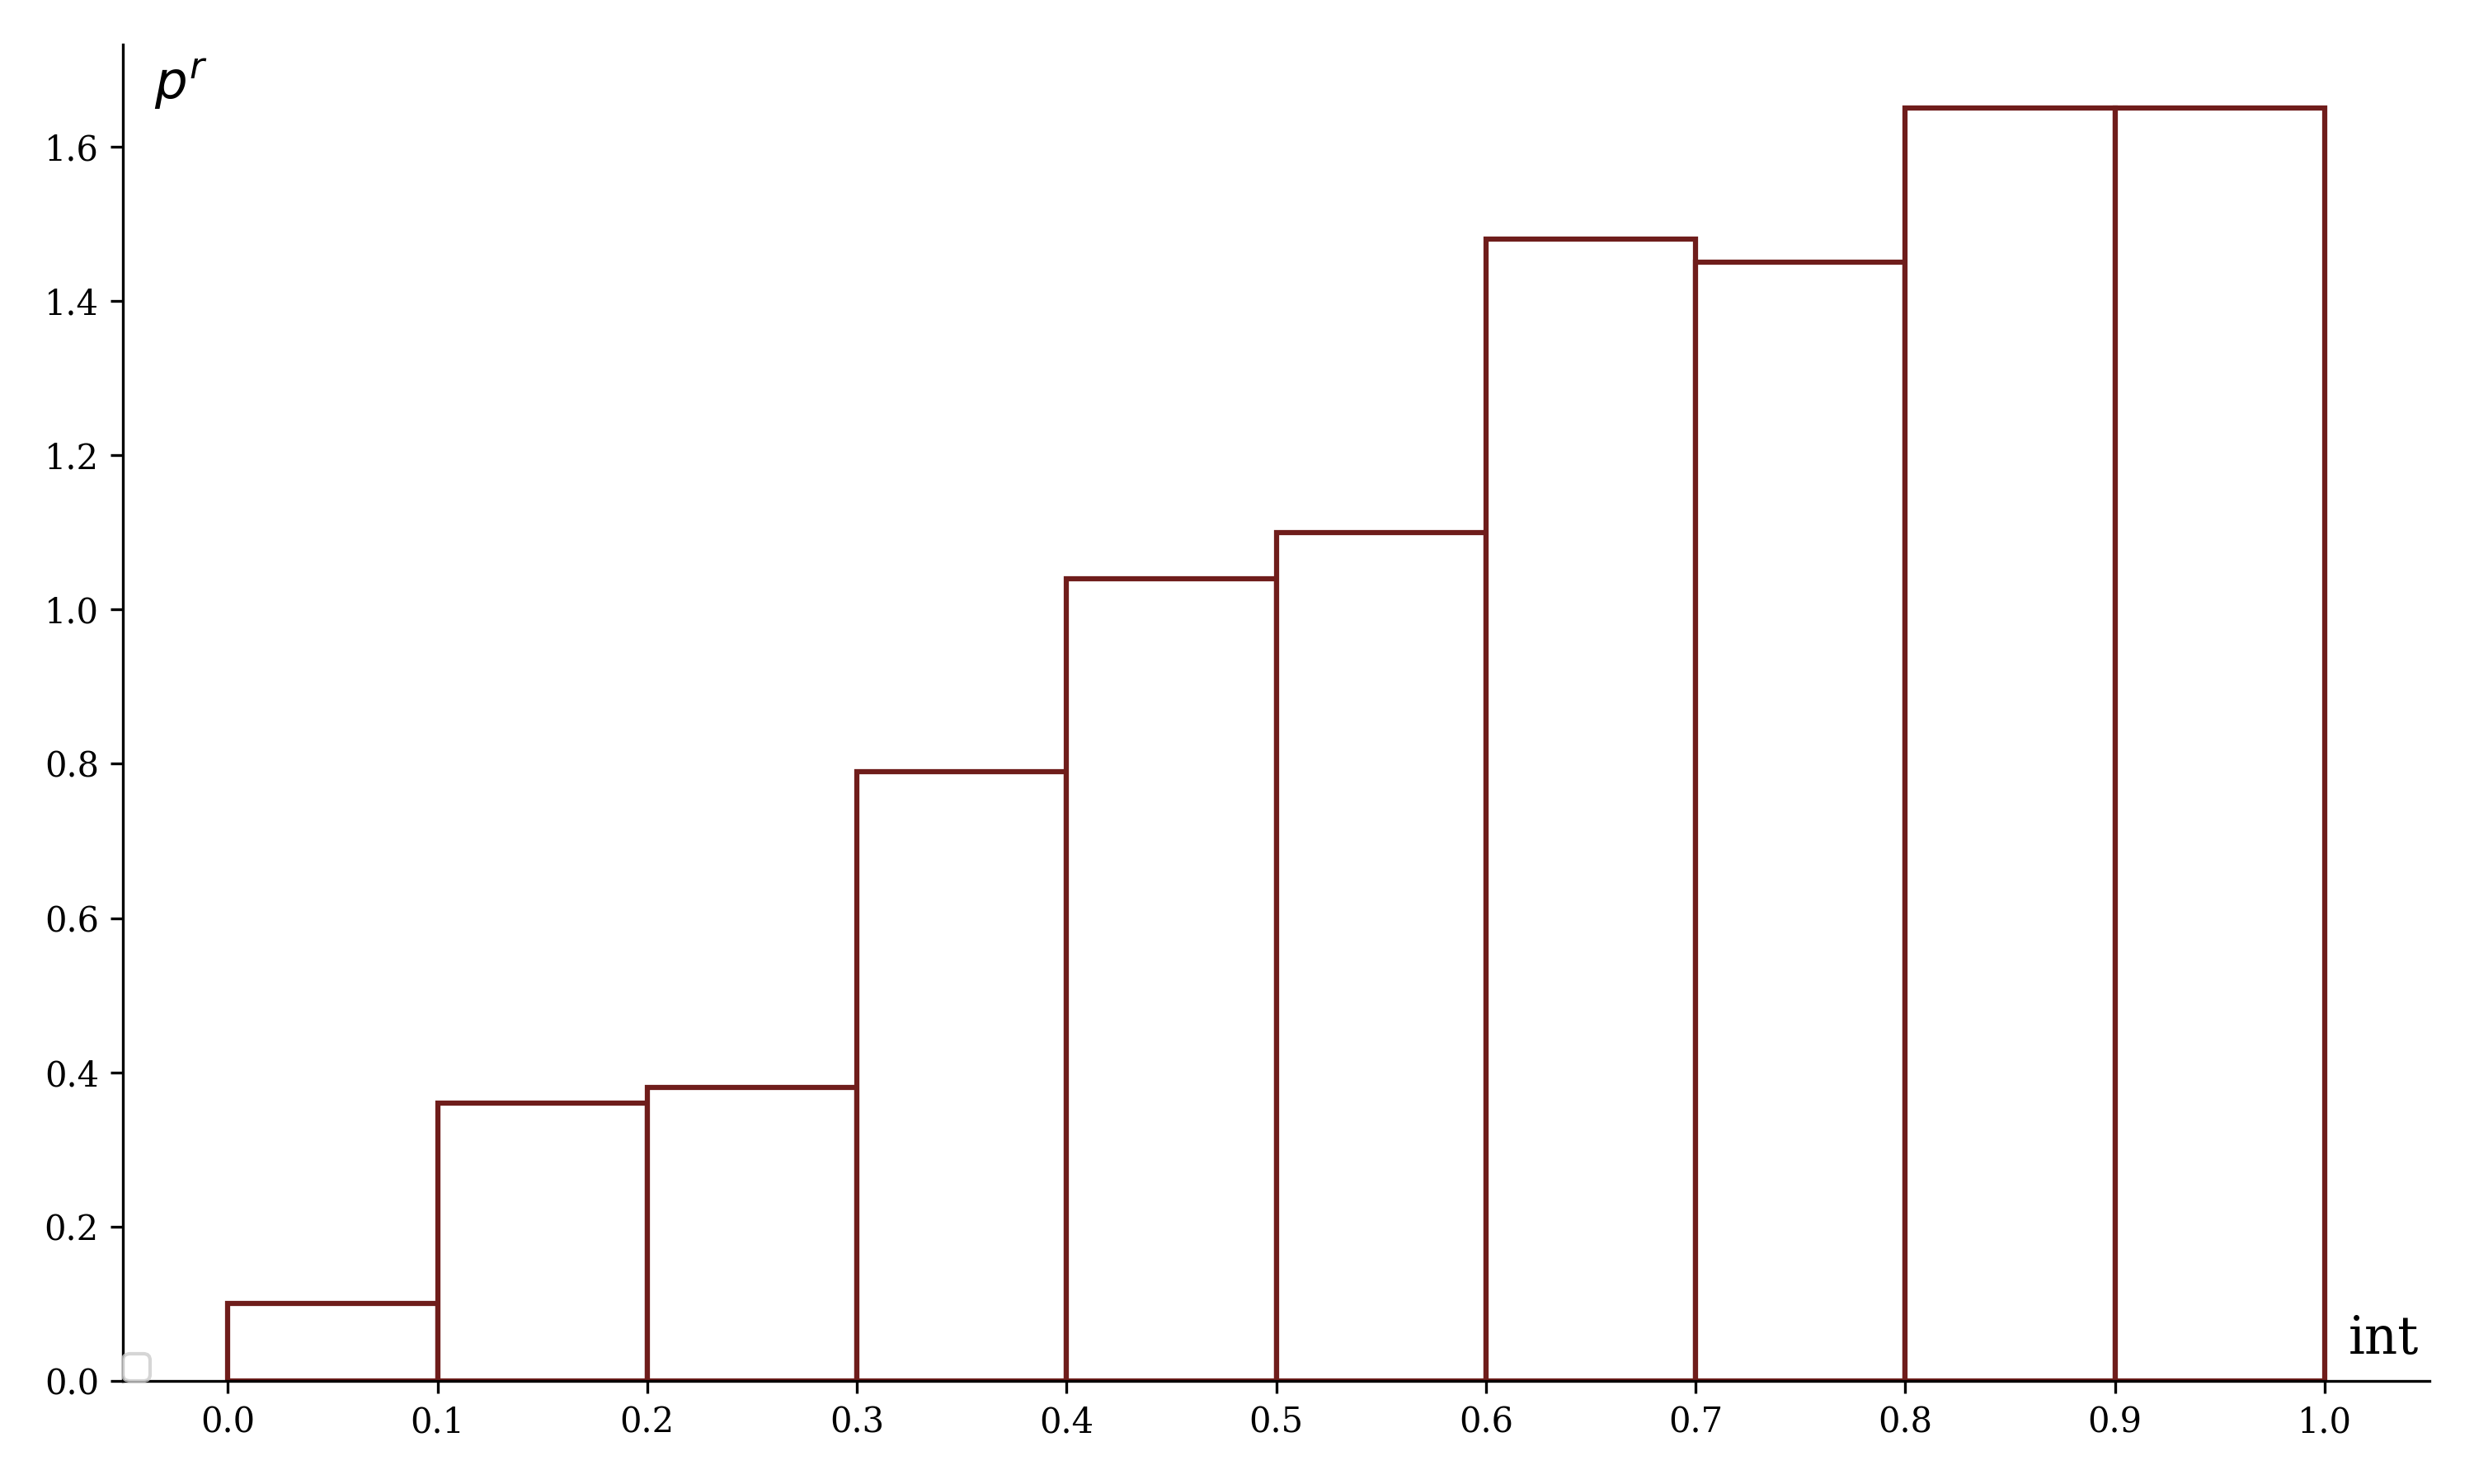
\includegraphics[width=\textwidth, height=\textheight, keepaspectratio]{sample35_hist}
\end{minipage}%
\begin{minipage}[t]{0.25\textwidth}
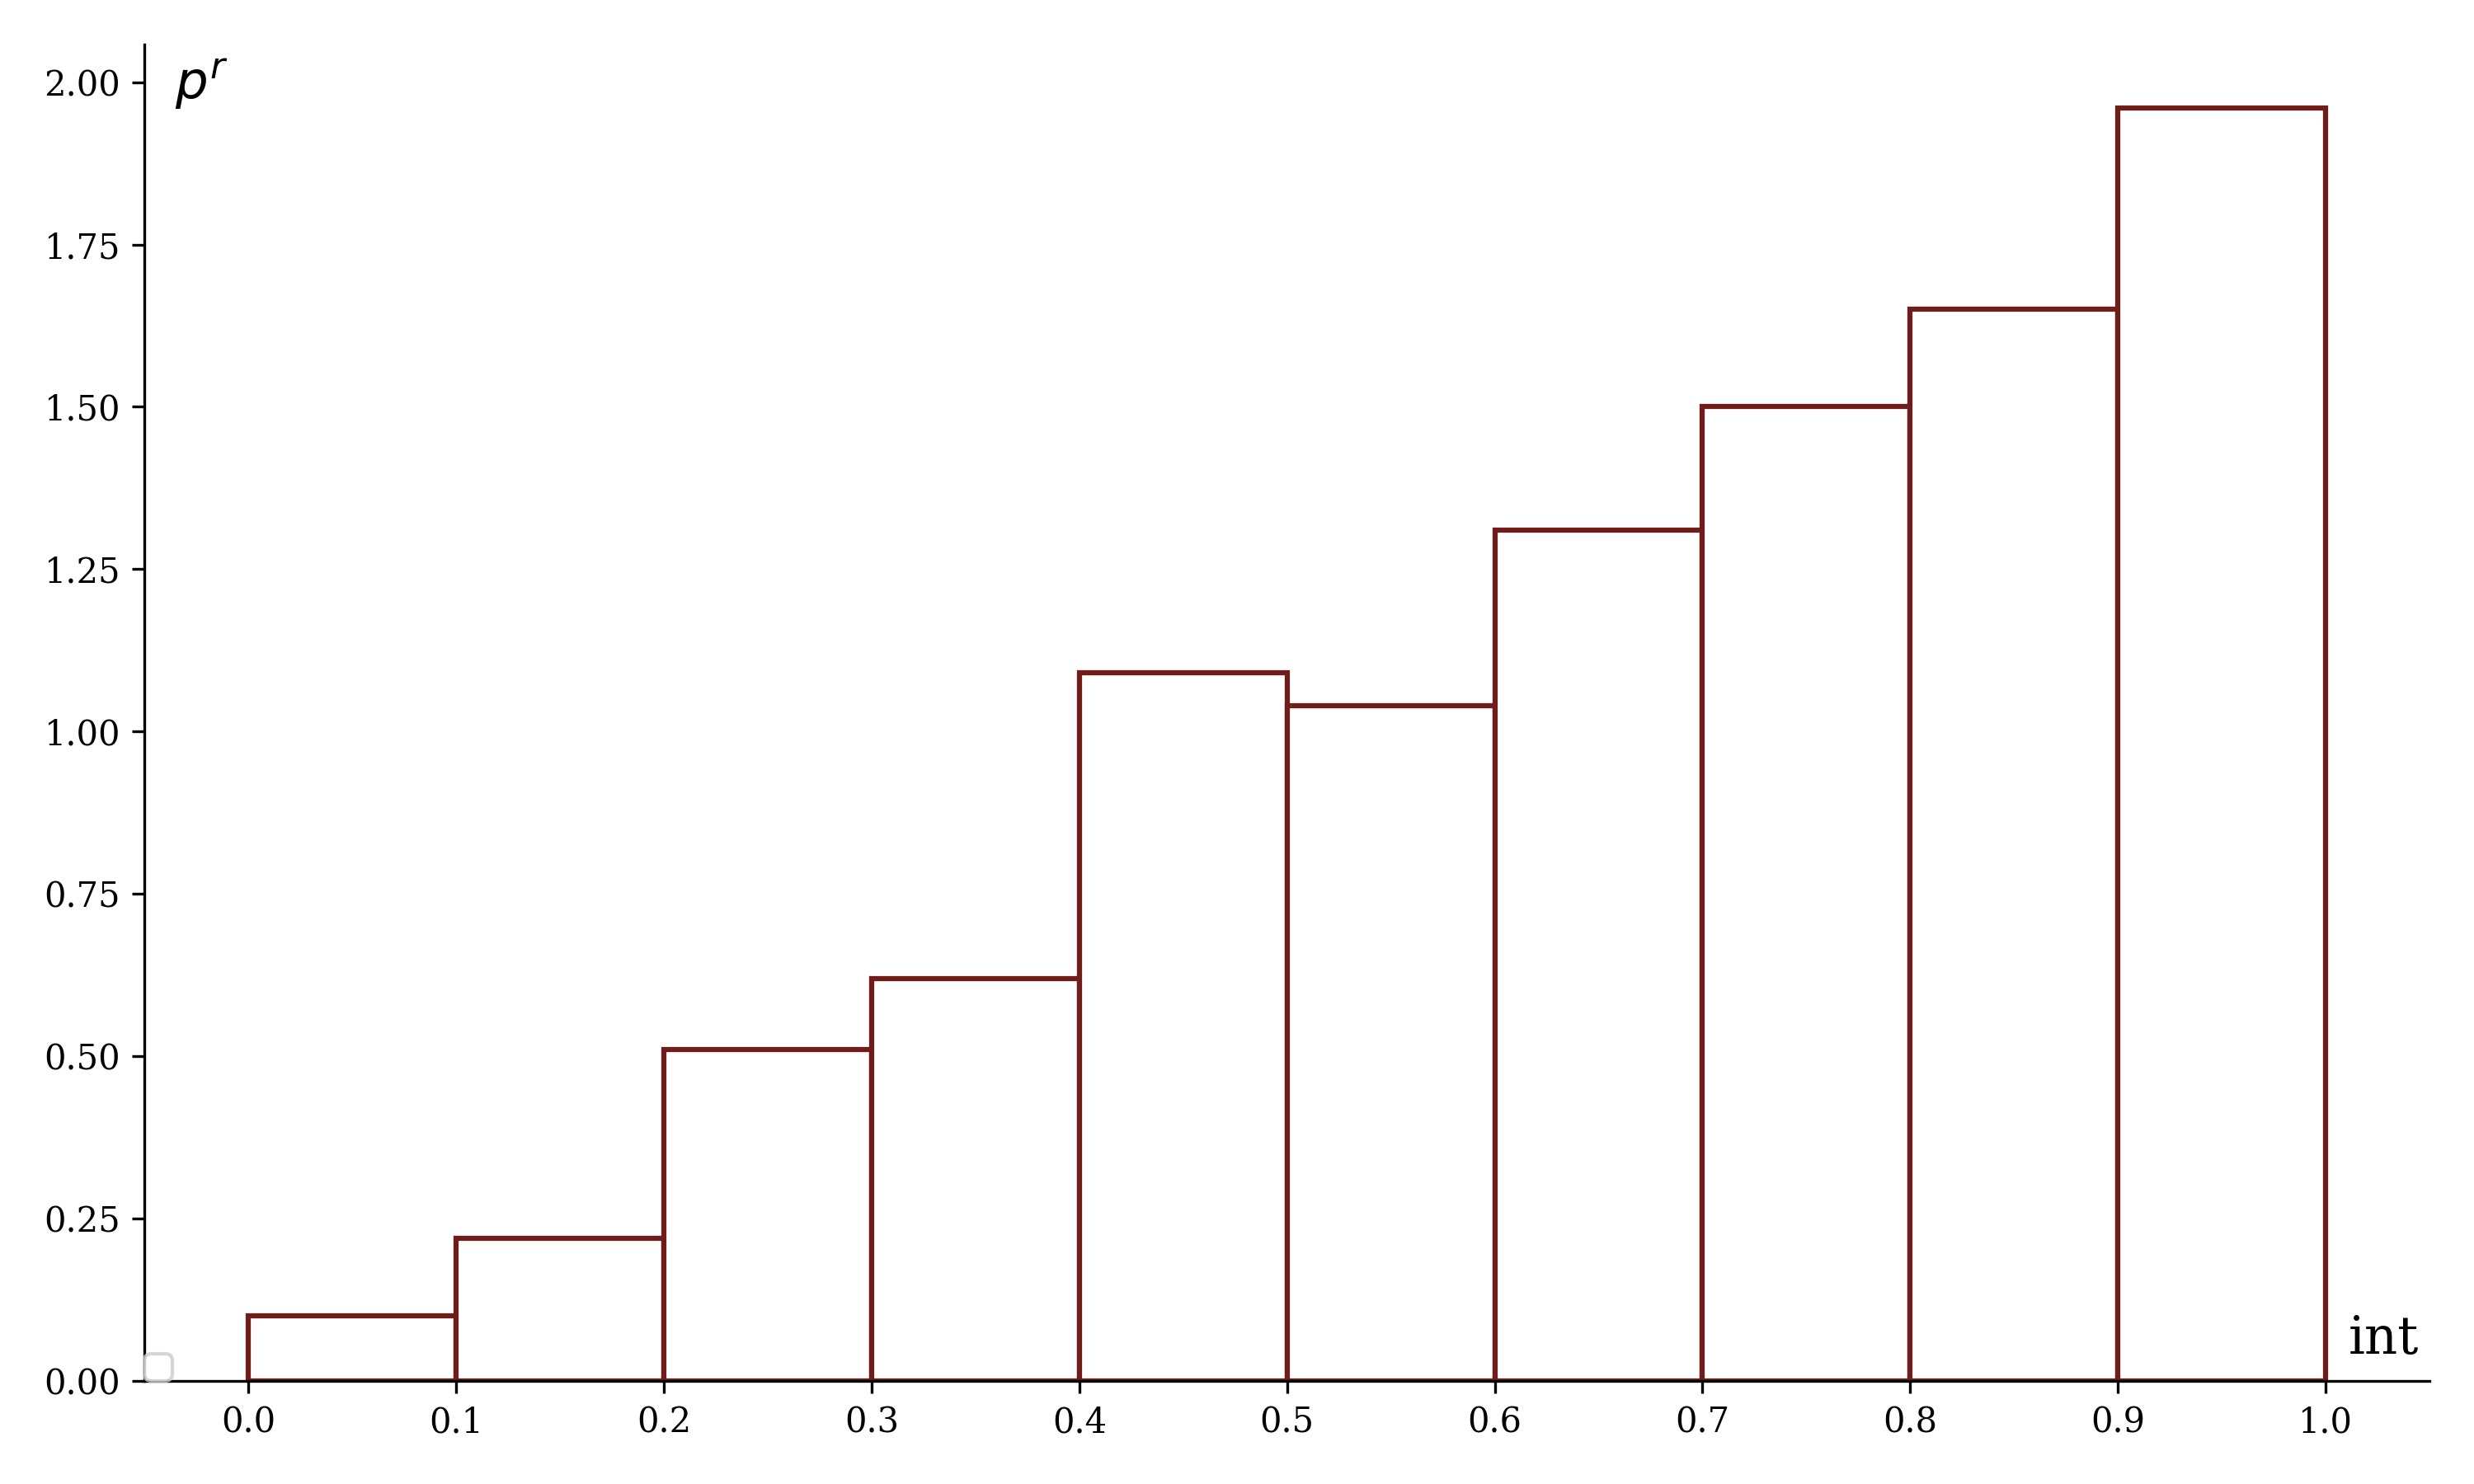
\includegraphics[width=\textwidth, height=\textheight, keepaspectratio]{sample36_hist}
\end{minipage}

\newpage\newgeometry{left=25mm, right=25mm, top=20mm, bottom=20mm}

Теперь перейдем к вычислению статистики $D_k(n, l)$.\\

Напишем вспомогательную функцию для выбора корректной метрики, в соответствии с вариантом:
\begin{center}
  \begin{lstlisting}[language=Python]
def metric(nu, p):
    nu = np.array(nu)
    p  = np.array(p)
    match D_:
        case 1:
            return 1/n_ * np.max(np.abs(nu - n_ * p))
        case 2:
            return 1/n_ * np.sum(np.abs(nu - n_ * p))
        case 3:
            return 1/n_ * np.sqrt(np.sum((nu - n_ * p)**2))
        case 4:
            return np.sum((np.abs(nu - n_ * p))/(n_ * p))
        case 5:
            return np.sum((nu - n_ * p)**2/(n_ * p * (n_ - n_ * p)))
  \end{lstlisting}
\end{center}

Количество значений, попавших в j-ый интервал группировки ($\nu$) нам уже известно и 
хранится в поле $\_freqs$ для каждого объекта класса \high{Sample}. \\

Теоретическую вероятность попадания в j-ый интервал группировки найдем в соответствии с 
(2):

\begin{center}
  \begin{lstlisting}[language=Python]
theorIntHitProbs_  = [] # p_j
theorIntHitProbsN_ = [] # n*p_j

for interval in Sample._intervals:
    beg = interval[0]
    end = interval[1]

    theorIntHitProb = cdf_(end) - cdf_(beg)
    theorIntHitProbs_.append(theorIntHitProb)

    theorIntHitProbsN_.append(Sample._n * theorIntHitProb)
  \end{lstlisting}
\end{center}

\begin{flalign*}
  & p: [0.01 \hspace{10pt} 0.03 \hspace{10pt} 0.05 \hspace{10pt} 0.07 \hspace{10pt} 0.09 \hspace{10pt} 0.11 \hspace{10pt} 0.13 \hspace{10pt} 0.15 \hspace{10pt} 0.17 \hspace{10pt} 0.19] \\
  & n \cdot p: [10.0 \hspace{10pt} 30.0 \hspace{10pt} 50.0 \hspace{10pt} 70.0 \hspace{10pt} 90.0 \hspace{10pt} 110.0 \hspace{10pt} 130.0 \hspace{10pt} 150.0 \hspace{10pt} 170.0 \hspace{10pt} 190.0] \\
\end{flalign*}

Наконец вычислим статистики:

\begin{center}
  \begin{lstlisting}[language=Python]
D_arr = []
for groupedSample in groupedSamples:
    nu = groupedSample._freqs
    D_curr = metric(nu, theorIntHitProbs_)

    D_arr.append(D_curr)
  \end{lstlisting}
\end{center}

Выведем первые и последние две статистики в отсортированном массиве статистик всех выборок:

\begin{equation*}
  [0.235165 \qquad 0.237748 \qquad ... \qquad 2.278528 \qquad 2.2851]
\end{equation*}

Теперь приблеженно оценим квантили уровней $\alpha = [0.1 \hspace{10pt} 0.05 \hspace{10pt} 0.01]$:

\begin{center}
  \begin{lstlisting}[language=Python]
alphas_ = [0.1, 0.05, 0.01]
quantiles_ = np.quantile(D_arr, [1 - alpha for alpha in alphas_], 
                                method='inverted_cdf')
quantiles_
  \end{lstlisting}
\end{center}

Получим:
\begin{table}[h!]
  \centering
  \renewcommand{\arraystretch}{1.5}
  \begin{tabular}{l|ccc}
  $\alpha$ & 0.1 & 0.05 & 0.01 \\
  \hline 
  $D_{cr}$ & 1.33 & 1.46 & 1.7
  \end{tabular}
\end{table}

Напишем еще одну вспомогательную функцию для тестирования построенного критерия:

\begin{center}
  \begin{lstlisting}[language=Python]
def testSample(sample):
    groupedSample = Sample(sample)
    nu = groupedSample._freqs
    D_curr = metric(nu, theorIntHitProbs_)

    accepted = 0
    accepted_sent = []
    for i, quantile in enumerate(quantiles_):
        if D_curr < quantile:
            accepted_text = f'{D_curr} < {quantile} for alpha: {alphas_[i]} => accept(alpha={alphas_[i]})\n'
            accepted_sent.append(accepted_text)
            accepted += 1

    if accepted == 3:
            print(f'{D_curr} < D for all alphas => accept')
    elif accepted > 0:
        print(accepted_sent)
    else:
        print(f'{D_curr} > D for all alphas => decline')
  \end{lstlisting}
\end{center}

\newpage

И запустим на нескольких законах распределения:

\begin{itemize}
  \item Uniform: $D \approx 14.226 > D_{cr}$ $\forall \alpha \in [0.1 \hspace{10pt} 0.05 \hspace{10pt} 0.01] \Rightarrow$ гипотеза отклоняется во всех случаях
  \item $\eta = \sqrt{\xi}, \hspace{10pt} \xi \sim \text{R}[0,1]$: $D \approx 1.203 < D_{cr}$ $\forall \alpha \in [0.1 \hspace{10pt} 0.05 \hspace{10pt} 0.01] \Rightarrow$ гипотеза принимается во всех случаях
  \item $\eta = 1 - \sqrt{\xi}, \hspace{10pt} \xi \sim \text{R}[0,1]$: $D \approx 30.992 > D_{cr}$ $\forall \alpha \in [0.1 \hspace{10pt} 0.05 \hspace{10pt} 0.01] \Rightarrow$ гипотеза отклоняется во всех случаях
  \item Beta: $D \approx 26.130 > D_{cr}$ $\forall \alpha \in [0.1 \hspace{10pt} 0.05 \hspace{10pt} 0.01] \Rightarrow$ гипотеза отклоняется во всех случаях
  \item Triangular: $D \approx 7.152 > D_{cr}$ $\forall \alpha \in [0.1 \hspace{10pt} 0.05 \hspace{10pt} 0.01] \Rightarrow$ гипотеза отклоняется во всех случаях
  \item Exponential (truncated to [0, 1]): $D \approx 21.886 > D_{cr}$ $\forall \alpha \in [0.1 \hspace{10pt} 0.05 \hspace{10pt} 0.01] \Rightarrow$ гипотеза отклоняется во всех случаях
  \item Lognormal (truncated to [0, 1]): $D \approx 6.101 > D_{cr}$ $\forall \alpha \in [0.1 \hspace{10pt} 0.05 \hspace{10pt} 0.01] \Rightarrow$ гипотеза отклоняется во всех случаях
  \item Weibull (truncated to [0, 1]): $D \approx 6.590 > D_{cr}$ $\forall \alpha \in [0.1 \hspace{10pt} 0.05 \hspace{10pt} 0.01] \Rightarrow$ гипотеза отклоняется во всех случаях
\end{itemize}

\section*{Вывод}\vspace{-20pt}\rule{\linewidth}{0.1mm}

На основе стохастического эксперимента был построен критерий согласия для проверки 
простой гипотезы. Критерий был проверен на семи выборках распределений не в соответствие 
с основной гипотезой, и для каждой из них основную гипотезу отклонил, что говорит в 
пользу критерия. Кроме того, критерий был проверен на выборке, распределенной в 
соответствие с основной гипотезой. Для этого случая была получена статистика, меньшая 
каждого из уровней доверия, и основная гипотеза была принята, что также говорит в пользу 
критерия.

% ---------------------------------------CODE---------------------------------------

\newpage

\section*{Приложение}\vspace{-20pt}\rule{\linewidth}{0.1mm}

Программный код, с помощью которого была выполнена данная лабораторная работа.\\

\begin{center}
  \begin{lstlisting}[language=Python]
import numpy as np
import scipy as sp
from dataclasses import dataclass, field
from typing import List, ClassVar
from IPython.display import Math, display
import matplotlib.pyplot as plt
from sklearn.manifold import TSNE

EXTRA_SAMPLE_SIZE = 1000
SAVE_PLOTS = False
FINITE_DIFFERENCE_APPROXIMATION_STEP_SIZE = 1e-6

A_ = 1
D_ = 4
n_ = 1000
m_ = 1e4

def generateValue(n=1):
    match A_:
        case 0:
            return sp.stats.uniform.rvs(size=n)
        case 1:
            return np.sqrt(sp.stats.uniform.rvs(size=n))
        case 2:
            return 1 - np.sqrt(sp.stats.uniform.rvs(size=n))

def metric(nu, p):
    nu = np.array(nu)
    p  = np.array(p)
    match D_:
        case 1:
            return 1/n_ * np.max(np.abs(nu - n_ * p))
        case 2:
            return 1/n_ * np.sum(np.abs(nu - n_ * p))
        case 3:
            return 1/n_ * np.sqrt(np.sum((nu - n_ * p)**2))
        case 4:
            return np.sum((np.abs(nu - n_ * p))/(n_ * p))
        case 5:
            return np.sum((nu - n_ * p)**2/(n_ * p * (n_ - n_ * p)))

m_ = int(m_)

a_ = 0
b_ = 1

def decorate_plot(ax, x_ticks, xname, yname, loc=(-0.025, -0.3)):
    SIZE_TICKS = 10

    # Eliminate upper and right axes
    ax.spines['right'].set_color('none')
    ax.spines['top'].set_color('none')

    # Show ticks in the left and lower axes only
    ax.xaxis.set_ticks_position('bottom')
    ax.yaxis.set_ticks_position('left')

    # axis names
    ax.set_xlabel(xname, fontsize=15)
    ax.xaxis.set_label_coords(0.98, 0.05)

    ax.set_ylabel(yname, rotation=0, fontsize=15)
    ax.yaxis.set_label_coords(0.025, 0.95)

    ax.set_xticks(x_ticks)

    # Adjust the font size of the tick labels
    ax.tick_params(axis='both', which='major', labelsize=SIZE_TICKS)

    plt.legend(fontsize=10, loc=loc)

    # Update font settings
    plt.rcParams.update({'font.family': 'serif', 'font.size': 12})

    # Adjust layout
    plt.tight_layout()

def clean(data):
    res = []
    for el in data:
        res.append(round(el, 3))
    return res

@dataclass
class Sample:
    # static fields
    _n:              ClassVar[int]         = None
    _min:            ClassVar[float]       = None
    _max:            ClassVar[float]       = None
    _range:          ClassVar[float]       = None
    _l:              ClassVar[float]       = None
    _h:              ClassVar[float]       = None
    _int_boundaries: ClassVar[List[float]] = None
    _intervals:      ClassVar[List[float]] = None
    _mid_ranges:     ClassVar[List[float]] = None

    # instance fields
    _freqs:             List[float] = field(default_factory=list)
    _rel_freqs:         List[float] = field(default_factory=list)
    _rel_freqs_density: List[float] = field(default_factory=list)

    @classmethod
    def _initializeStaticFields(cls):
        cls._n     = n_
        cls._min   = a_
        cls._max   = b_
        cls._range = cls._max - cls._min
        cls._l     = 1 + int(np.log2(cls._n))
        cls._h     = cls._range / cls._l
        
        cls._int_boundaries = np.array(
            [cls._min + i * cls._h for i in range(0, cls._l + 1, 1)]
        )
        cls._intervals = np.array(
            [(cls._int_boundaries[i], cls._int_boundaries[i+1]) for i in range(0, cls._l, 1)]
        )
        cls._mid_ranges = np.array(
            [sum(interval)/2 for interval in cls._intervals]
        )

    def _countFrequencies(self, data):
        present = lambda el, int_ : int_[0] <= el < int_[1]
        freqs_ = np.zeros(Sample._l)
        for el in data:
            for j in range(0, Sample._l, 1):
                if present(el, Sample._intervals[j]):
                    freqs_[j] += 1 
        freqs_[-1] += np.count_nonzero(data == Sample._max)

        self._freqs = freqs_
        self._postCountFrequencies()

    def _postCountFrequencies(self):
        if self._freqs is not None:
            rel_freqs_ = self._freqs / Sample._n

            self._rel_freqs = rel_freqs_

            rel_freqs_density_ = self._rel_freqs / Sample._h
            self._rel_freqs_density = rel_freqs_density_

    def _hist(self, filename):
        RED = '#6F1D1B'

        _, ax = plt.subplots(figsize=(10, 6))

        x_values = Sample._mid_ranges
        y_values = self._rel_freqs_density

        ax.bar(x_values, 
               y_values, 
               width=Sample._h, 
               color='white',
               edgecolor=RED, 
               linestyle='-', 
               linewidth=1.5, 
               align='center')

        decorate_plot(ax, Sample._int_boundaries, 'int', '$p^r$', loc=(0, 0))

        # if SAVE_PLOTS:
        plt.savefig(f'{filename}.png', dpi=300, transparent=True)

        plt.show()

    def __init__(self, data):
        if self._n is None:
            self._initializeStaticFields()

        self._countFrequencies(data)

    def __str__(self) -> str:
        str_: str = f'n: {self._n}\n'                                              \
                    f'min: {self._min}     max: {self._max}\n'                     \
                    f'range: {self._range}\n'                                      \
                    f'l: {self._l}\n'                                              \
                    f'h: {self._h}\n'                                              \
                    f'interval boundaries: {self._int_boundaries}\n'               \
                    f'intervals: {self._intervals}\n'                              \
                    f'intervals\' midpoints: {self._mid_ranges}\n'                 \
                    f'frequencies: {self._freqs}\n'                                \
                    f'relative frequencies: {self._rel_freqs}\n'                   \
                    f'relative frequencies\' density: {self._rel_freqs_density}\n' \
                    
        return str_

class CDM:
    def __init__(self, h):
        self.h = h
    
    def diff(self, f, x):
        numerator = f(x + self.h) - f(x - self.h)
        denominator = 2 * self.h

        return numerator / denominator
  
cdm_ = CDM(h=FINITE_DIFFERENCE_APPROXIMATION_STEP_SIZE)

def buildBar(filename):
    RED = '#6F1D1B'

    _, ax = plt.subplots(figsize=(10, 6))

    interval_size = b_ - a_
    step = interval_size/5

    x_values = [sp.stats.uniform.rvs() for _ in range(EXTRA_SAMPLE_SIZE)]
    y_values = [sp.stats.uniform.rvs() for _ in range(EXTRA_SAMPLE_SIZE)]

    colors = [sp.stats.uniform.rvs(0, 100) for _ in range(EXTRA_SAMPLE_SIZE)]

    ax.scatter(x_values, 
               y_values, 
               c=colors, 
               cmap='Reds',
               label='')

    ax.axvline(x=b_, color='black', linestyle='--')
    ax.axhline(y=b_, color='black', linestyle='--')

    ax.axvline(x=a_, color='black', linestyle='--')
    ax.axhline(y=a_, color='black', linestyle='--')

    ax.axhline(y=b_ + step, color='white', linestyle='--')

    ax.set_title(f'$\\xi \\sim R[{a_}, {b_}]$')

    decorate_plot(ax, np.arange(a_, b_ + step + step, step), '', '', loc='best')

    if SAVE_PLOTS:
        plt.savefig(f'{filename}.png', dpi=300, transparent=True)

    plt.show()

buildBar('uniform_EXTRA_SAMPLE_SIZE')

def buildBar(filename):
    RED = '#6F1D1B'

    _, ax = plt.subplots(figsize=(10, 6))

    interval_size = b_ - a_
    step = interval_size/5

    x_values = generateValue(n=EXTRA_SAMPLE_SIZE)
    y_values = generateValue(n=EXTRA_SAMPLE_SIZE)

    colors = [sp.stats.uniform.rvs(0, 100) for _ in range(EXTRA_SAMPLE_SIZE)]

    plotTitle = ''
    match A_:
        case 1:
            plotTitle = '$\\eta = \\sqrt{\\xi}, \\xi \\sim R[0, 1]$'
        case 2:
            plotTitle = '$1 - \\eta = \\sqrt{\\xi}, \\xi \\sim R[0, 1]$'

    ax.scatter(x_values, 
               y_values, 
               c=colors, 
               cmap='Reds',
               label='')
    
    ax.axvline(x=b_, color='black', linestyle='--')
    ax.axhline(y=b_, color='black', linestyle='--')

    ax.axvline(x=a_, color='black', linestyle='--')
    ax.axhline(y=a_, color='black', linestyle='--')

    ax.axhline(y=b_ + step, color='white', linestyle='--')

    ax.set_title(plotTitle)

    decorate_plot(ax, np.arange(a_, b_ + step + step, step), '', '', loc='best')
    
    if SAVE_PLOTS:
        plt.savefig(f'{filename}.png', dpi=300, transparent=True)

    plt.show()

if A_ != 0:
    buildBar('modifed_uniform_EXTRA_SAMPLE_SIZE')

    def g(x):
    match A_:
        case 1:
            return np.sqrt(x)
        case 2:
            return 1 - np.sqrt(x)
        case _:
            raise ValueError("Invalid value for A")

def inverseFunction(y):
    def equation_to_solve(x):
            return g(x) - y

    sol = None
    guesses = np.arange(a_, b_ + (b_ - a_)/10, (b_ - a_)/10)
    for guess in guesses:
        try: 
            sol, = sp.optimize.fsolve(equation_to_solve, guess)
            break
        except:
            continue
    
    if sol is not None: 
        return sol
    else: 
        raise Exception('solution was not found')

def pdf_(x):
    if x < a_ or x > b_:
        return 0

    def numericalDerivative(f, x):
         return cdm_.diff(f=f, x=x)
    
    inverse_x = inverseFunction(x)
    if A_ == 2: # ???
        return np.abs(1/numericalDerivative(g, inverse_x) * sp.stats.uniform.pdf(inverse_x))
    else:
        return 1 / numericalDerivative(g, inverse_x) * sp.stats.uniform.pdf(inverse_x)

def cdf_(x):
    if A_ == 2: # ???
        return 1 - sp.stats.uniform.cdf(inverseFunction(x))
    else:
        return sp.stats.uniform.cdf(inverseFunction(x))

def buildBar(filename):
    RED = '#6F1D1B'

    _, ax = plt.subplots(figsize=(10, 6))

    interval_size = b_ - a_
    beg = a_ - (b_ - a_)
    end = b_ + (b_ - a_)
    step = interval_size/5

    x_values = np.linspace(beg, end, EXTRA_SAMPLE_SIZE)
    y_values = sp.stats.uniform.pdf(x_values)

    ax.scatter(x_values, 
               y_values, 
               color=RED, 
               label='',
               s=1)

    plt.grid(linestyle='-', linewidth=0.25)

    ax.set_title('$f_\\xi(x)$')

    decorate_plot(ax, np.arange(beg, end + step, step), '', '', loc='best')

    if SAVE_PLOTS:
        plt.savefig(f'{filename}.png', dpi=300, transparent=True)

    plt.show()

buildBar('uniform_pdf')

def buildBar(filename):
    RED = '#6F1D1B'

    _, ax = plt.subplots(figsize=(10, 6))

    interval_size = b_ - a_
    beg = a_ - (b_ - a_)
    end = b_ + (b_ - a_)
    step = interval_size/5

    x_values = np.linspace(beg, end, EXTRA_SAMPLE_SIZE)
    y_values = sp.stats.uniform.cdf(x_values)

    ax.plot(x_values, 
            y_values, 
            color=RED, 
            label='')

    plt.grid(linestyle='-', linewidth=0.25)

    ax.set_title('$F_\\xi(x)$')

    decorate_plot(ax, np.arange(beg, end + step, step), '', '', loc='best')

    if SAVE_PLOTS:
        plt.savefig(f'{filename}.png', dpi=300, transparent=True)

    plt.show()

buildBar('uniform_cdf')

def buildBar(filename):
    RED = '#6F1D1B'

    _, ax = plt.subplots(figsize=(10, 6))

    interval_size = b_ - a_
    beg = a_ - (b_ - a_)
    end = b_ + (b_ - a_)
    step = interval_size/5
 
    x_values = np.linspace(beg, end, EXTRA_SAMPLE_SIZE * 10)
    y_values = [pdf_(x) for x in x_values]

    ax.scatter(x_values, 
               y_values, 
               color=RED, 
               label='',
               s=1)

    plt.grid(linestyle='-', linewidth=0.25)

    ax.set_title('$f_\\eta(x)$')

    decorate_plot(ax, np.arange(beg, end + step, step), '', '', loc='best')

    if SAVE_PLOTS:
        plt.savefig(f'{filename}.png', dpi=300, transparent=True)

    plt.show()

if A_ != 0:
    buildBar('modified_uniform_pdf')

def buildBar(filename):
    RED = '#6F1D1B'

    _, ax = plt.subplots(figsize=(10, 6))

    interval_size = b_ - a_
    beg = a_ - (b_ - a_)
    end = b_ + (b_ - a_)
    step = interval_size/5

    x_values = np.linspace(beg, end, EXTRA_SAMPLE_SIZE)
    y_values = [cdf_(x) for x in x_values]

    ax.plot(x_values, 
            y_values, 
            color=RED, 
            label='')

    plt.grid(linestyle='-', linewidth=0.25)

    ax.set_title('$F_\\eta(x)$')

    decorate_plot(ax, np.arange(beg, end + step, step), '', '', loc='best')

    if SAVE_PLOTS:
        plt.savefig(f'{filename}.png', dpi=300, transparent=True)

    plt.show()

if A_ != 0:
    buildBar('modifed_uniform_cdf')

data_ = [generateValue(n_) for _ in range(m_)]

groupedSamples = [Sample(sample) for sample in data_]

for sample in groupedSamples:
    print(sample)
    print('-'*200,end='\n\n')

for i, grouped_sample in enumerate(groupedSamples):
    grouped_sample._hist(f'sample{i}_hist')

theorIntHitProbs_  = [] # p_j
theorIntHitProbsN_ = [] # n*p_j

for interval in Sample._intervals:
    beg = interval[0]
    end = interval[1]

    theorIntHitProb = cdf_(end) - cdf_(beg)
    theorIntHitProbs_.append(theorIntHitProb)

    theorIntHitProbsN_.append(Sample._n * theorIntHitProb)

print(f'p_i: {clean(theorIntHitProbs_)}')
print(f'n * p_i: {clean(theorIntHitProbsN_)}')

D_arr = []
for groupedSample in groupedSamples:
    nu = groupedSample._freqs
    D_curr = metric(nu, theorIntHitProbs_)

    D_arr.append(D_curr)

sorted_D_arr = sorted(D_arr)
print(sorted_D_arr[0], sorted_D_arr[1], sorted_D_arr[-2], sorted_D_arr[-1])

alphas_ = [0.1, 0.05, 0.01]
quantiles_ = np.quantile(D_arr, [1 - alpha for alpha in alphas_], method='inverted_cdf')
quantiles_

def testSample(sample):
    groupedSample = Sample(sample)
    nu = groupedSample._freqs
    D_curr = metric(nu, theorIntHitProbs_)

    accepted = 0
    accepted_sent = []
    for i, quantile in enumerate(quantiles_):
        if D_curr < quantile:
            accepted_text = f'{D_curr} < {quantile} for alpha: {alphas_[i]} => accept(alpha={alphas_[i]})\n'
            accepted_sent.append(accepted_text)
            accepted += 1

    if accepted == 3:
            print(f'{D_curr} < D for all alphas => accept')
    elif accepted > 0:
        print(accepted_sent)
    else:
        print(f'{D_curr} > D for all alphas => decline')

sample_uniform = sp.stats.uniform.rvs(size=n_)
display(Math(f'$\\begin{{equation}} \\text{{Uniform}} \\end{{equation}}$'))
testSample(sample_uniform)


sample_modifed_uniform1 = np.sqrt(sp.stats.uniform.rvs(size=n_))
display(Math(f'$\\begin{{equation}} \\eta = \\sqrt{{\\xi}}, \\xi \\sim R[0, 1] \\end{{equation}}$'))
testSample(sample_modifed_uniform1)


sample_modifed_uniform2 = 1 - np.sqrt(sp.stats.uniform.rvs(size=n_))
display(Math(f'$\\begin{{equation}} \\eta = 1 - \\sqrt{{\\xi}}, \\xi \\sim R[0, 1] \\end{{equation}}$'))
testSample(sample_modifed_uniform2)


alpha = 2
beta_param = 5

sample_beta = sp.stats.beta.rvs(alpha, beta_param, size=n_)
display(Math(f'$\\begin{{equation}} \\text{{Beta}} \\end{{equation}}$'))
testSample(sample_beta)


c = 0.5

sample_triangular = sp.stats.triang.rvs(c, size=n_)
display(Math(f'$\\begin{{equation}} \\text{{Triangular}} \\end{{equation}}$'))
testSample(sample_triangular)


lambda_param = 1.0
b = 1.0 

sample_trunc_exponential = sp.stats.truncexpon.rvs(b, scale=1/lambda_param, size=n_)
display(Math(f'$\\begin{{equation}} \\text{{Exponential (truncated to [0, 1])}} \\end{{equation}}$'))
testSample(sample_trunc_exponential)


s = 0.5 
scale = np.exp(0) 

samples_lognormal = sp.stats.lognorm.rvs(s, scale=scale, size=n_)
samples_lognormal_truncated = [x for x in samples_lognormal if a_ <= x <= b_]
display(Math(f'$\\begin{{equation}} \\text{{Lognormal  (truncated to [0, 1])}} \\end{{equation}}$'))
testSample(samples_lognormal_truncated)


shape = 1.5
scale = 1.0

samples_weibull = sp.stats.weibull_min.rvs(shape, scale=scale, size=n_)
samples_weibull_truncated = [x for x in samples_weibull if a_ <= x <= b_]
display(Math(f'$\\begin{{equation}} \\text{{Weibull  (truncated to [0, 1])}} \\end{{equation}}$'))
testSample(samples_weibull_truncated)
  \end{lstlisting}
\end{center}

\newpage

\section*{Список использованных источников}\vspace{-20pt}\rule{\linewidth}{0.1mm}

\begin{enumerate}
  \item Севастьянов Б.А. Курс теории вероятностей и математической статистики. --Москва-Ижевск, 2019. - 95с
\end{enumerate}

\end{document}
